% eilmer3-user-guide.tex
% PJ, March 2007 -- elmer2 version
%     September 2008 -- eilmer3 version
%
\documentclass[12pt,a4paper,twoside]{article}
\usepackage[body={16cm,24.5cm}]{geometry}
\usepackage{hyperref}
\hypersetup{colorlinks=true,linkcolor=blue}
\usepackage{graphicx}
\usepackage{makeidx}
% \usepackage{showidx}
\usepackage{listings}
\usepackage{lscape}
\usepackage{longtable}
\usepackage{amsmath}
\usepackage{subfig}
\lstset{basicstyle=\ttfamily\scriptsize,identifierstyle=,keywordstyle=}

%------------------------------------------------------------------
% a couple horizontal bars to delimit embedded code
% the width suits the page size set above and
% the mathmode eliminates spaces between the three elements
\newcommand{\topbar}{\ensuremath{
    \rule{0.1mm}{2.0mm} \rule[2.0mm]{159.5mm}{0.1mm} \rule{0.1mm}{2.0mm}
}}
\newcommand{\bottombar}{\ensuremath{
    \rule{0.1mm}{2.0mm} \rule{159.5mm}{0.1mm} \rule{0.1mm}{2.0mm}
}}
\newcommand{\topbarshort}{\ensuremath{
    \rule{0.1mm}{2.0mm} \rule[2.0mm]{149.5mm}{0.1mm} \rule{0.1mm}{2.0mm}
}}
\newcommand{\bottombarshort}{\ensuremath{
    \rule{0.1mm}{2.0mm} \rule{149.5mm}{0.1mm} \rule{0.1mm}{2.0mm}
}}
%------------------------------------------------------------------

\title{
    The Eilmer3 Code: User Guide and Example Book.
}
\author{
    Mechanical Engineering Report 2008/07\\
    P. A. Jacobs\thanks{Queensland Geothermal Energy Centre of Excellence, The University of Queensland, Brisbane, Australia.} 
    and 
    R. J. Gollan\thanks{Centre for Hypersonics, The University of Queensland, Brisbane, Australia.}\\
    {\normalsize with contributions\thanks{These contributions have come in the form of examples, debugging, 
    proof-reading and constructive comments on the codes and this document, and code for special cases.}
    from a cast of many, including:}\\
    {\normalsize Peter Blyton,}
    {\normalsize Arianna Bosco,}
    {\normalsize Djamel Boutamine,}
    {\normalsize Laurie Brown,}
    {\normalsize David Buttsworth,} \\
    {\normalsize Wilson Chan,} 
    {\normalsize Sam Chiu,}
    {\normalsize Chris Craddock,} 
    {\normalsize Brian Cook,} 
    {\normalsize Jason Czapla,} \\
    {\normalsize Carlos de Miranda-Ventura,} 
    {\normalsize Andrew Denman,} 
    {\normalsize David Gildfind,} 
    {\normalsize Richard Gooze\'{e},}
    {\normalsize Stefan Hess,} \\
    {\normalsize Carolyn Jacobs,} 
    {\normalsize Ian Johnston,}
    {\normalsize Ojas Joshi,}
    {\normalsize Rainer Kirchhartz,} 
    {\normalsize Matt McGilvray,} \\
    {\normalsize David Mee,} 
    {\normalsize Luke Montgomery,} 
    {\normalsize Jan-Pieter Nap,} 
    {\normalsize Brendan O'Flaherty,} 
    {\normalsize Paul Petrie-Repar,} \\
    {\normalsize Dan Potter,} 
    {\normalsize Deepak Ramanath,}
    {\normalsize Michael Scott,}
    {\normalsize Umar Sheikh,} 
    {\normalsize Ben Stewart,} \\
    {\normalsize Joseph Tang,} 
    {\normalsize Katsu Tanimizu,} 
    {\normalsize Paul van der Laan,} 
    {\normalsize Jaidev Vesudevan,} 
    {\normalsize Mike Wendt,} \\
    {\normalsize Vince Wheatley,} 
    {\normalsize Adrian Window,} 
    {\normalsize Hannes Wojciak,}
    {\normalsize Fabian Zander}
}
% \date{September 2008}
\makeindex

\begin{document}
\maketitle

% For some reason, the abstract environment causes the labelling in
% the metapost figures to disappear; strange!
% \begin{abstract}
% \end{abstract}
\centerline{\textbf{Preface}}
Eilmer3 is an integrated collection of programs for the simulation of transient,
compressible flow in two and three spatial dimensions.
It provides a preparation program that can be used to set up a database of
simulation parameters, a block-structured grid defining the flow domain and an
initial flow field.
These items are then used as a starting point for the main simulation program
which computes a series of snapshots of the evolving flow.
Eilmer3 is part of the larger collection of compressible flow simulation codes
found at \url{http://www.mech.uq.edu.au/cfcfd/}.

\medskip
This user guide contains a collection of example simulations: scripts, results
and commentary.
It may be convenient for new users of the code to identify an example
close to the situation that they wish to model and then adapt the 
scripts for that example.

\cleardoublepage
\tableofcontents

%------------------------------------------------------------------
\cleardoublepage
\baselineskip = 1.5pc

\part{User guide}

\section{Introduction}
%
Eilmer3 is an integrated collection of programs for the simulation of transient,
compressible flow in two and three dimensions.
It provides a preparation program (\texttt{e3prep.py}) that can be used to set up a database of
simulation parameters, a block-structured, body-fitted grid defining the flow domain and an
initial flow field.
These items are then used as a starting point for the main simulation program (\texttt{e3shared.exe})
which computes a series of snapshots of the evolving flow.
Finally, a rudimentary but versatile postprocessing program (\texttt{e3post.py}) makes the flow data
available for further analysis.

\medskip
Eilmer3 is a derivative of the code mbcns2 which, in turn was an experiment in writing
the mb\_cns code in C++.
Once it was determined that there were clear benefits in using C++,
our three-dimensional flow code Elmer was then reworked in C++ as Elmer2.
At the same time, we experimented with using the Python language for the user's input script and 
embedding the Lua language in order to make some of the boundary conditions programmable.
Of course, these codes being experiments in C++, we soon decided that it could all be done
much more cleanly and be made much more versatile if we just reworked some of the basic modules.
Thus, the thermochemistry was reworked and the separate two and three dimensional codes merged
into Eilmer3.
The name change is to avoid a naming clash with the Elmer finite-element code 
from Finland.\footnote{\url{http://www.csc.fi/elmer}}

\medskip 
The following sections provide example input scripts and shell scripts for a number of simulations.
These are intended to be starting points for your own simulations and should be studied together with 
the other manuals that can be found in the documentation section of the 
Compressible Flow CFD Group web site:  
\url{http://www.mech.uq.edu.au/cfcfd/}.\index{Internet address}
Study these scripts carefully; some of the interesting bits of the documentation are
embedded within them.

\medskip
For a description of the methods coded into \texttt{Eilmer3}, see the companion report \cite{jacobs_etal_2010b}
which covers the gas-dynamic formulation and the basic thermochemistry components.

\clearpage
%------------------------------------------------------------------
\section{Building and installing the programs}
%
The core solver and its modules are mainly written in C/C++ for speed and the benefits of compile time checking. 
The pre- and post-processing programs are mainly Python so that we get flexibility and convenient customization.
There is also a little Tcl/Tk and Lua.

\medskip
Our main development environment is Linux but the programs can be deployed on
Linux, flavours of Unix such as MacOS-X and MS-Windows (using Cygwin).
The main requirement is that the C/C++ compilers, the Tcl and Python
interpreters be available, along with their supporting libraries and 
various extensions. 
The source code of the Lua interpreter is included in with Eilmer3.
The reStructuredText file \texttt{eilmer3.rst} (Appendix\,\ref{getting-started-file}) 
or the corresponding HTML file from the web site\footnote{The web site 
\url{http://www.mech.uq.edu.au/cfcfd/} has a nicely formatted set of instructions,
detailed API documents that have been extracted from the source code and 
a number of examples.  It is regularly expanded and updated.}
provides more detail including 
the actual commands needed to build and install the programs.

\medskip
If you are not accustomed to working with Unix/Linux, 
have a look at Appendix\,\ref{linux-command-notes-sec}
for a brief introduction to working on the command line.


%------------------------------------------------------------------
\section{Running simulations}
%
Setting up a simulation is mostly an exercise in writing a text-based 
description of your flow and its bounding geometry.
This \textit{input script} is presented to the preparation program as 
a Python source file, often with the extension ``.py''.
Once you have prepared your flow specification as an input script using your favourite text editor, 
the simulation data is generated by the \texttt{Eilmer3} programs in a number of stages:
\begin{itemize}
\item[1] Create the geometry definition, a grid and the initial flow state.
  For simple to moderately complex geometries, the built-in geometry tools (described later in this manual)
  are adequate.
  For complex geometries, you may find it convenient to import block-structured grids, 
  possibly from a specialized gridding tool such as \texttt{Gridgen} or \texttt{ICEMCFD}.
\item[2] Run the simulation code to produce flow data at subsequent times.
\item[3] Reformat the flow solution data to produce files suitable for a data viewing program such as Paraview or GNU-Plot.
\end{itemize}

\newpage
\subsection{Data preparation (with e3prep.py)}
Create the geometry definition and a grid with the command\\
         \texttt{\$ e3prep.py --job=\textit{job} --do-svg }\\ \index{e3prep.py!using}\index{preparation}
         \vspace{0.25cm} \\
         \centerline{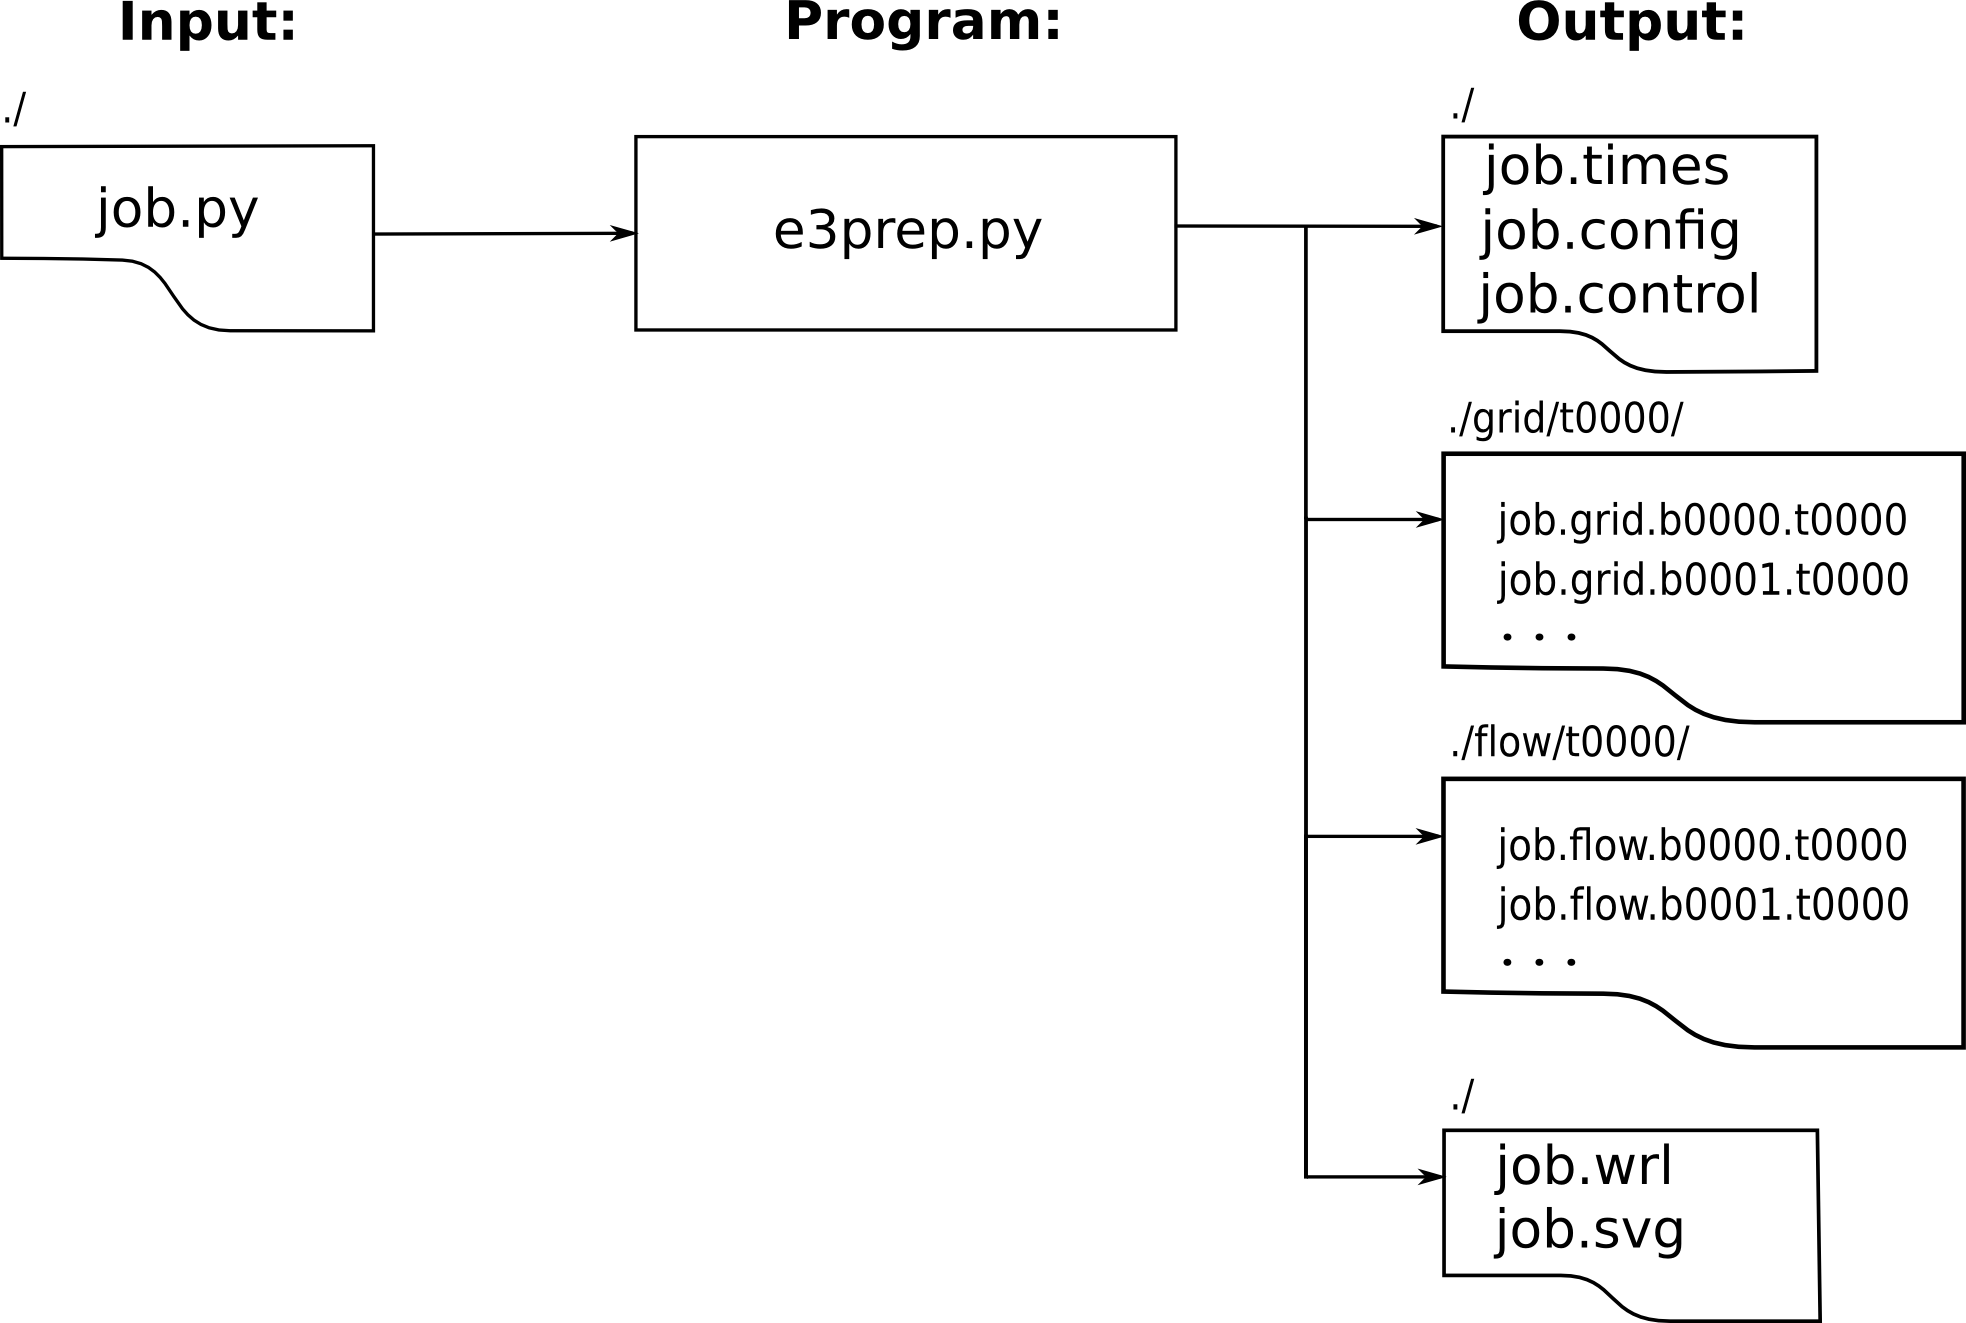
\includegraphics[width=0.7\textwidth]{figs/preparation.png}}\\
         The italics word \textit{job} in the command should be replaced 
         by whatever job name that you have chosen.
         That name is then used as a base to derive specific names for each of
         the files associated with the simulation.
         At a minimum, you have an input script called \textit{job}\texttt{.py} 
         with the \texttt{.py} extension, indicating that the script is written in Python.
         The files from the preparation stage are:
         \begin{itemize}
           \item \textit{job}\texttt{.config}: \index{config file}
             A database of configuration parameters in INI format.
             Parameters are specified, one per line, as \textit{parameter-name = value}.
             A hierarchical structure is given to the set of parameters via
             named subsections in the file.
             Although you would probably never assemble one of these parameter files
             from scratch manually, it is sometimes convenient to alter a value or two and rerun
             a simulation without invoking \texttt{e3prep.py}.
           \item \textit{job}\texttt{.control}: \index{control file}
             A small database of parameters to control the time-stepping, the final time,
             and the intervals between writing of solutions and history data.
             The content of this file is also in INI format and it is parsed at the
             start of every time step.
             This way, a user can alter the simulation behaviour (by editing this file)
             without having to restart the simulation.
             To stop a simulation cleanly, set the \texttt{halt\_now} entry to 1.\index{halting a simulation}
             Other control parameters are marked with \ddag~ in Section\,\ref{sec:sim-control-parameters}.
           \item  \textit{job}\texttt{.times}:
             A mapping of time stamps to actual times at which the simulation
             data was written.
             After the preparation stage, there should be only the zero-time entry.
           \item \textit{job}\texttt{.svg} or \textit{job}\texttt{.wrl}: \index{SVG} \index{VRML}
             Sometimes it is convenient to see a graphical representation of the flow domain 
             and boundary conditions.
             These options produce a SVG or VRML rendering of the block boundaries 
             and the boundary-condition labels.
             The \texttt{--do-svg} will invoke the rendering of two-dimensional blocks
             to a scalable-vector-graphics file while \texttt{--do-vrml} will render 
             three-dimensional blocks to a virtual-reality-modeling-language file.
             For two-dimensional simulations, the SVG file can be edited in a program such as \texttt{Inkscape}
             (\url{http://www.inkscape.org})
             and the result used as part of your documentation for a particular simulation.
           \item \textit{job}\texttt{.grid.b0000.t0000}, \textit{job}\texttt{.grid.b0001.t0000} :
             The grid of finite-volume cells, 
             one file for each block that defines part of the flow domain.
             The grids are written as plain text files in a relatively simple format.
             The spatial coordinates for points within each file are
             associated with cell vertices of the structured grid.\footnote{Note that, in recent versions of the programs, 
             the grid and flow files are written to subdirectories within the job directory.}
           \item one flow-data file for each block:
             \textit{job}\texttt{.flow.b0000.t0000}, \textit{job}\texttt{.flow.b0001.t0000}, ...
             containing the initial flow state within each of the finite-volume cells.
             Look at the first couple of lines of a flow file to see what data elements are written for each cell.
             Variable names appear on the second line and units are \texttt{SI}.
         \end{itemize}
         Note that the grid and flow data files are written to subdirectories of the same names.
         The grid is written once (at time zero, subdirectory \texttt{grid/t0000/}) and 
         the flow files are written to a new subdirectory (\texttt{flow/tnnnn/}) at each output time.
         This is to keep the main job directory clean and to allow easy copying or moving of 
         individual solution times.
         Also, these files are stored in ``gzip'' format with a ``.gz'' extension by default.\index{gzip}

\newpage
\subsection{Running the simulation (with e3shared.exe)} 
Run the simulation code to produce flow data at subsequent times.\footnote{If the simulation
finishes too quickly (possibly without taking any steps at all),
it may be that the initial time step size is too large and the calculation is unstable.
One symptom of this is that the final value for \texttt{dt} is reported as being
the excessively large value of \texttt{1e+6} seconds.
Choose a suitably small value and try again.}\\ \index{e3shared.exe!running a simulation}
         \texttt{\$ e3shared.exe --job=\textit{job} --run}\\
         \vspace{0.25cm} \\
         \centerline{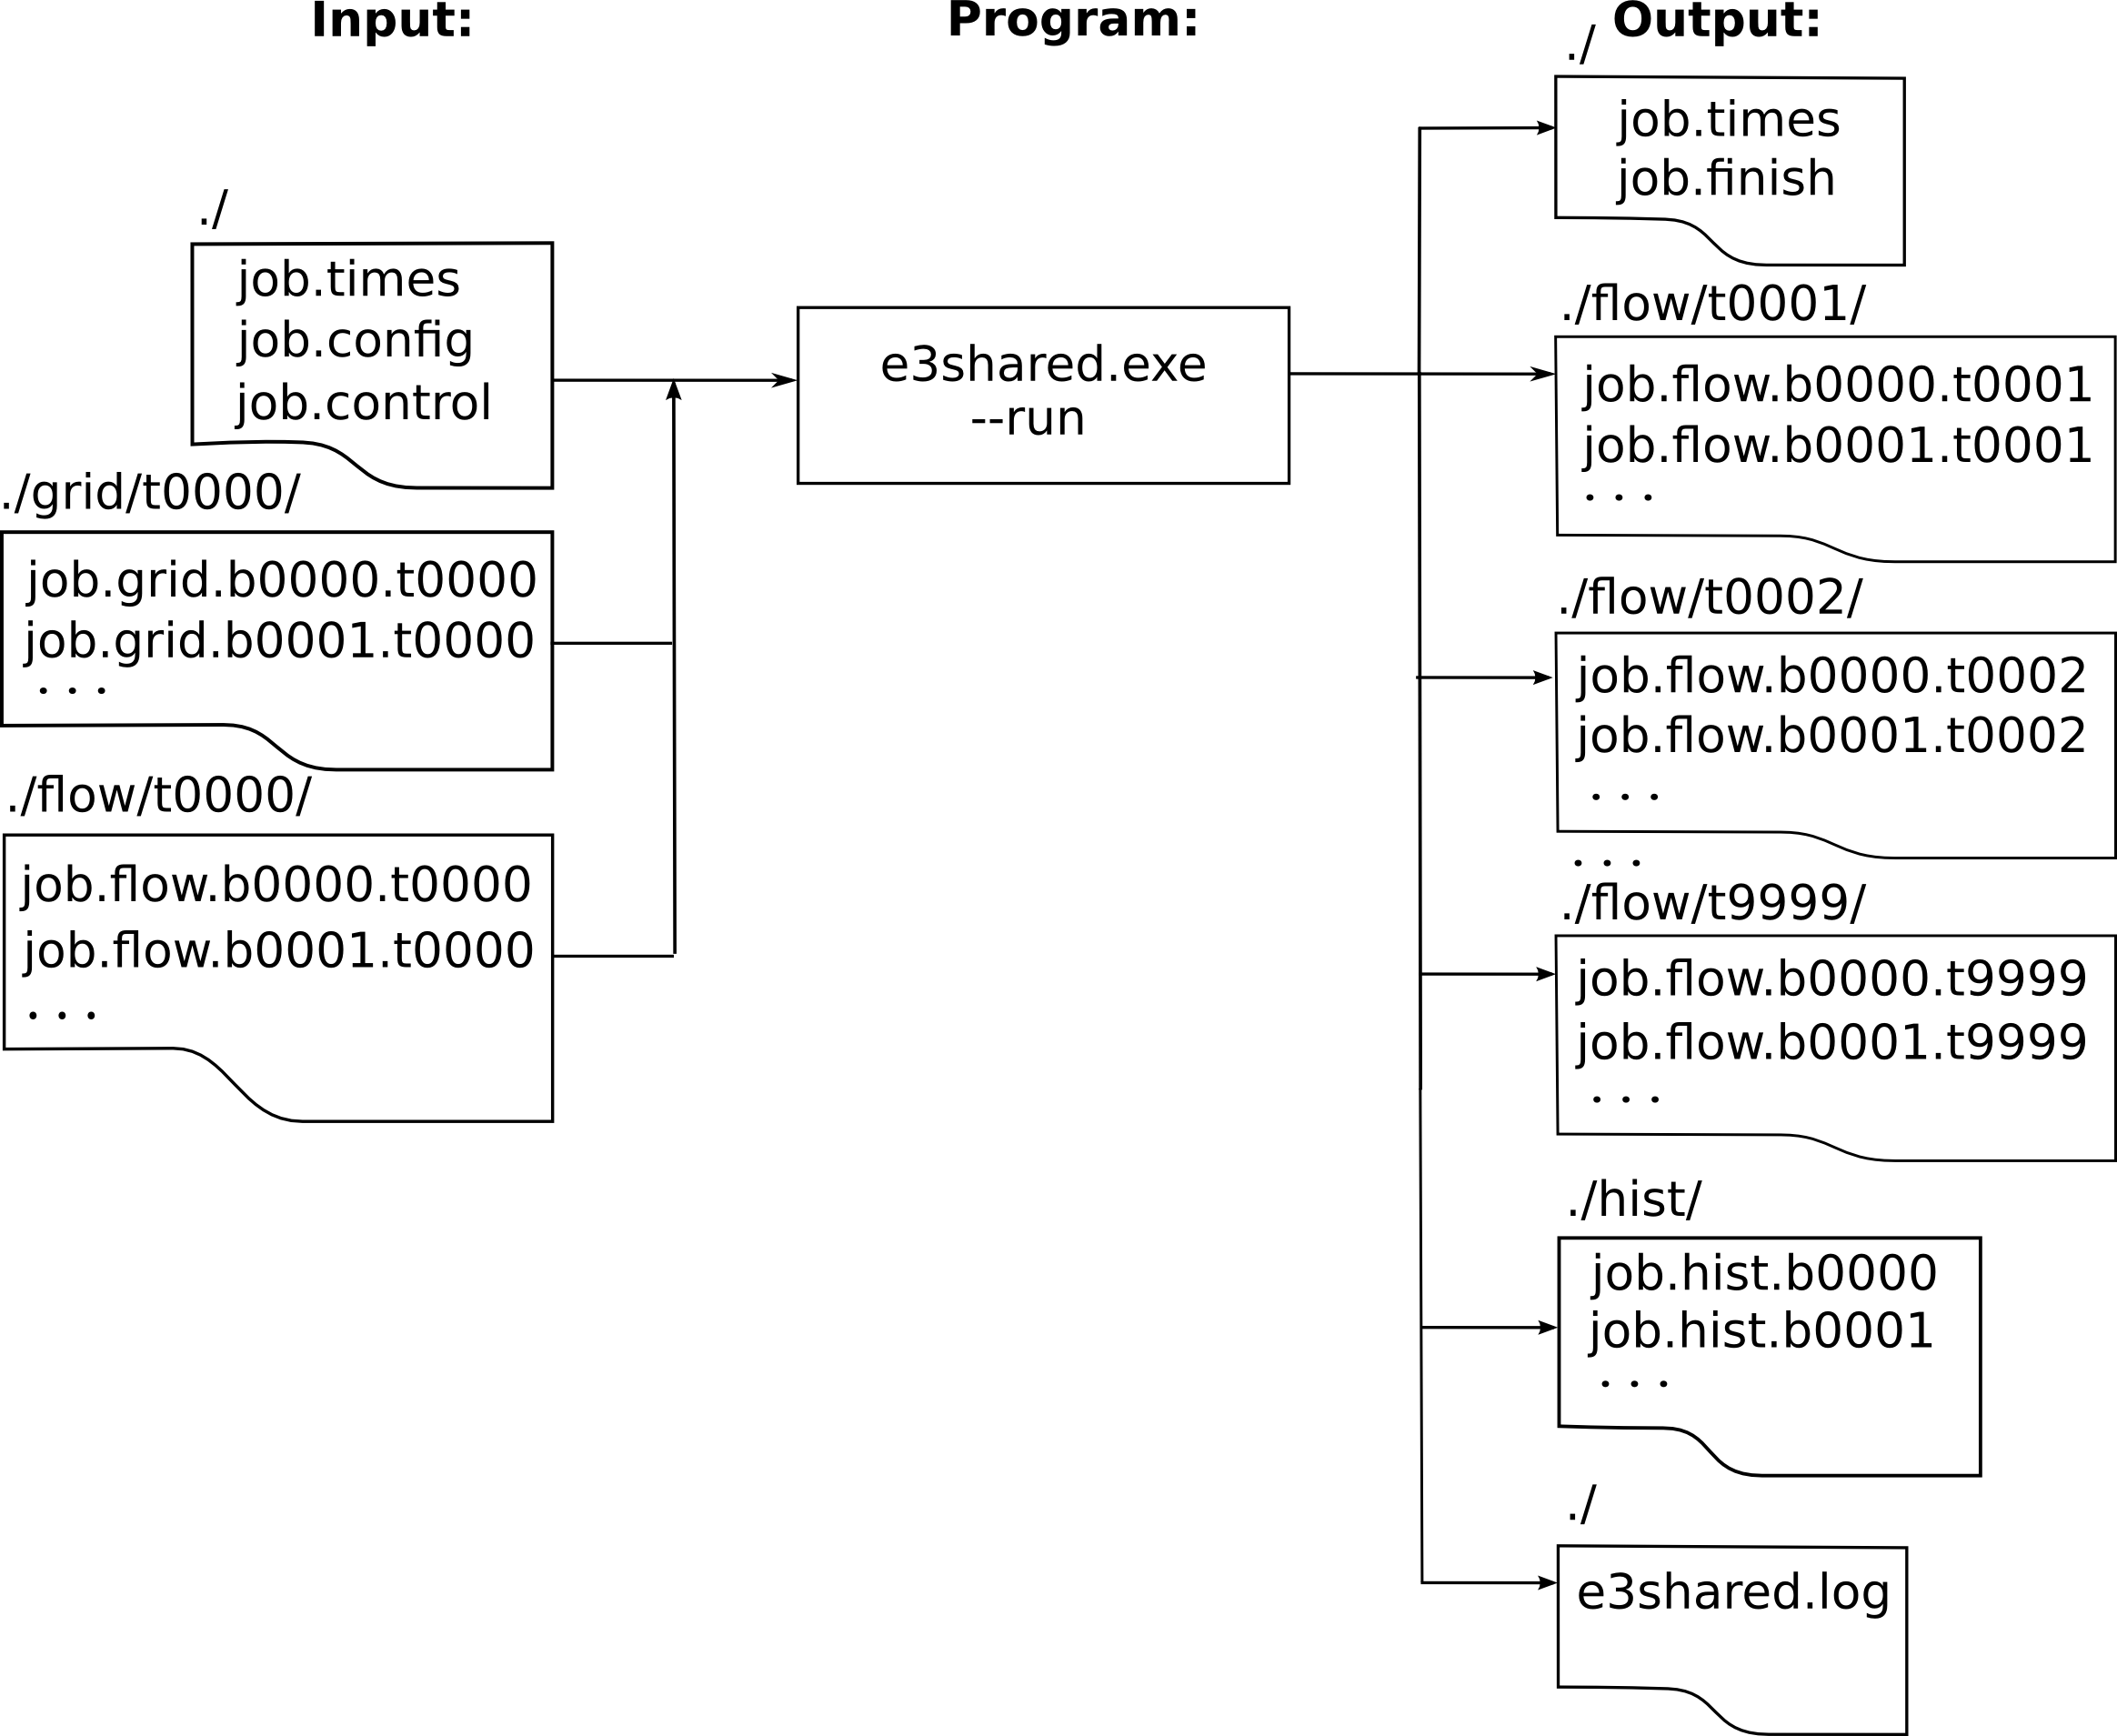
\includegraphics[width=0.7\textwidth]{figs/running-sim.png}}\\
         The output files are:
         \begin{itemize}
           \item \textit{job}\texttt{.flow.b}\textit{nnnn}\texttt{.t}\textit{mmmm}:
             The flow data for all cells at the times requested.
             As the simulation proceeds, whole-field solutions are written
             to new files with \textit{nnnn} representing the block number and
             \textit{mmmm} representing a time stamp.
             Look up the \textit{job}\texttt{.times} file to see what time values
             belong to each time stamp (or tindx).
             Just as for the grid files, each flow solution file is written 
             as a plain text file with a simple layout, not too different from 
             the Tecplot point-format for a structured-block grid.
             In these files, the spatial coordinates of points within the file are
             associated with the cell centres.
           \item  \textit{job}\texttt{.hist.b}\textit{nnnn}: \index{history location}
             Data at particular ``history locations'' and at times requested.
             This data is typically used to simulate the signals recorded by pressure 
             and heat-transfer sensors mounted on model surfaces.
             When restarting a simulation, the program will append to existing history files 
             rather than clobbering them.
             Note that, if you are running a simulation from the start multiple times, 
             you will need to manually remove the history files before each run.  
             The command \texttt{``rm -r ./hist/''} should do the job.
           \item  \textit{job}\texttt{.times}: \index{times file}
             A mapping of time stamps to actual times at which the simulation
             data was written.
             The main simulation appends lines to this file.
             This file may assist when automating some of the postprocessing operations.
           \item  \textit{job}\texttt{.finish}: \index{finish file}
             An INI-format file giving some information about the time-stepping parameters
             at the end of the simulation.
             These may be useful for starting a follow-on simulation.
         \end{itemize}

\medskip
For viscous simulations, surface heat flux and cell Reynolds number files are also written to the subdirectory \texttt{heat}.
See the \texttt{--heat-flux-list} option in Section\,\ref{sec:e3post} for a hint at how to extract the data and then
have a look in the data files to see what specific data has been captured. 

\subsection{Running the simulation in parallel (e3mpi.exe)}
%
One can build and run the distributed-memory version of the program, 
\texttt{e3mpi.exe}\index{e3mpi.exe}, on computers with 
the MPI (Message Passing Interface) library\footnote{See, for example, \url{http://www.open-mpi.org/}.} 
and runtime environment.
The notes in Appendix\,\ref{getting-started-file} show how to build and run 
the Eilmer3 executable for OpenMPI.\footnote{These notes are also available in HTML form at the URL
\url{http://www.mech.uq.edu.au/cfcfd/}.}
To run Eilmer3 across multiple processors\index{e3mpi.exe!running a simulation}
on a local machine use the following command\\
\texttt{\$ mpirun -np \textit{n} e3mpi.exe --job=name --run}\\
where \textit{n} is the number of MPI processes to use.
Note that the program is written such that one MPI process is assigned to each block; 
the number of MPI processes \emph{must} match the number of blocks in the simulation.
Each of these MPI processes is a separate program and you may run more than one per core 
or physical processor, however, if you want the shortest calculation time and you had lots of cores,
you would probably run one per core.

\subsection{Restarting a simulation}\index{restarting a simulation}
%
By default, the simulation program picks up the flow solution for \texttt{tindx} equal to 0 but
it can be told to pick up any other \texttt{tindx} snapshot.
To pick up a solution and continue, it is probably best to do a little house-keeping with the command\\
\texttt{\$ e3post.py --job=name --prepare-restart}\\
This renames the 9999 flow files and tidies up the \textit{job}\texttt{.times} file to reflect the changes.
Then you should edit the \textit{job}\texttt{.control} file and change the parameters \texttt{dt}
\texttt{max\_time} and \texttt{max\_steps} to suitable values.
Do \underline{not} run \texttt{e3prep.py} again, else it will write all over 
your newly edited \textit{job}\texttt{.control} file.
At this point, you should be ready to run the main simulation program again.
Remember to supply the relevant \texttt{tindx} value on the command line for your restart.
For example:\\
\texttt{\$ e3shared.exe --job=name --tindx=5 --run}

\medskip
Also, with restarts, be careful that you have consistent modelling requirements and settings.
Restarting a laminar simulation as a turbulent simulation with the $k-\omega$ model would lead
to inconsistent data.
It may be better to start a new job and use \texttt{ExistingSolution} objects\footnote{We need to make \texttt{ExistingSolution} smart enough to fill in missing values.} (see Section\,\ref{sec:ExistingSolution}) to pick up the old data. 

\newpage
\subsection{Postprocessing (with e3post.py)}\index{postprocessing} 
\label{sec:e3post}
%
Postprocessing of the simulation data is the most unstructured of the simulation activities.
We provide a postprocessing program, \texttt{e3post.py} that has the basic capabilities of picking up 
the simulation data and writing flow field files in formats suitable for 
\texttt{Paraview}, \texttt{Visit}, \texttt{Tecplot}, the venerable \texttt{Plot3D} or 
\texttt{gnuplot}\footnote{See the web sites  \url{http://www.paraview.org}, \url{https://wci.llnl.gov/codes/visit/},
\url{http://www.tecplot.com}, \url{http://people.nas.nasa.gov/\~rogers/plot3d/intro.html} and \url{http://www.gnuplot.info}}.
\vspace{0.25cm} \\
\centerline{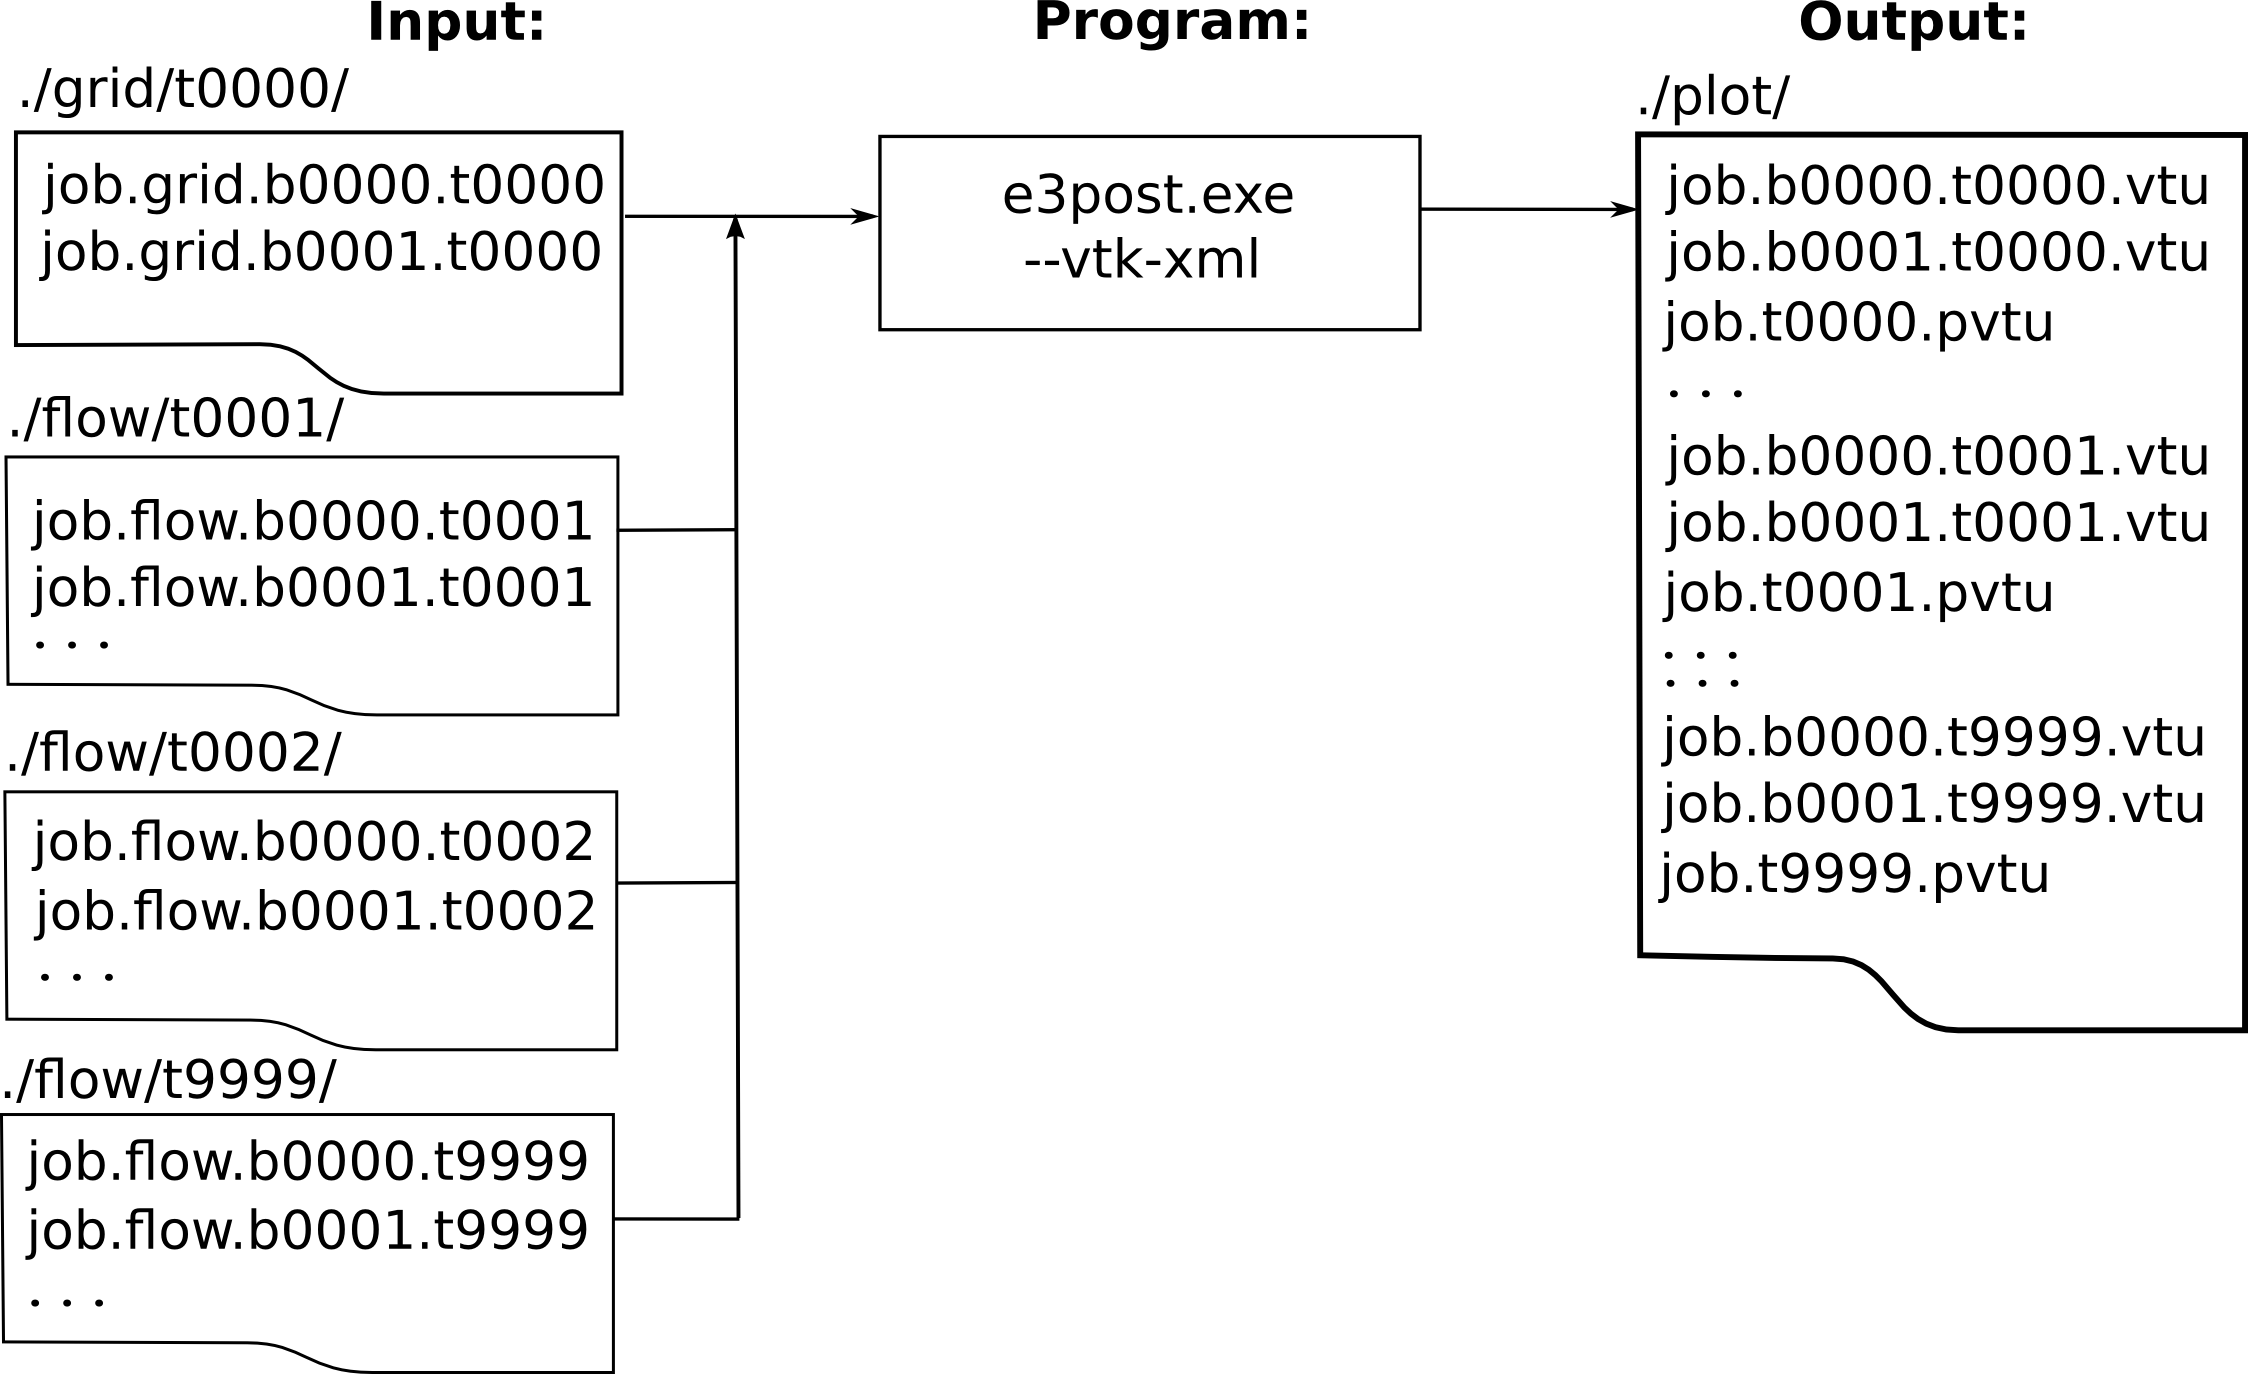
\includegraphics[width=0.7\textwidth]{figs/post-process.png}}\\

\medskip
To reformat the flow solution data into one unstructured grid
containing all of the flow data for the domain and write this data in a format suitable
for \texttt{Paraview} or \texttt{Visit}, use the command:\\
\texttt{\$ e3post.py --job=\textit{job} --vtk-xml --tindx=all}\\ \index{e3post.py!using}

\medskip
The postprocessing program (\texttt{e3\_post.py}) started as a fairly simple script that picked up solution data
and reformatted it for plotting, however, it has continued to sprout features and has become a bit 
complex to describe.
To see its command-line options, just run it without any options at all.
It should then print a \textit{usage} message which provides some hints.
As at October 2009, the start of this message is:

\noindent
{\footnotesize
\begin{verbatim}
Begin e3post.py...

Usage: e3post.py [--help] [--job=<jobFileName>] [--tindx=<index|all>]
                 [--zip-files|--no-zip-files]
                 [--vtk-xml] [--tecplot] [--plot3d]
                 [--prepare-restart] [--prepare-fstc-restart]
                 [--put-into-folders]
                 [--ref-function=<python-script>]
                 [--report-norms]
                 [--per-block-norm-list="jb,var-name,norm-name;..."
                 [--global-norm-list="var-name,norm-name;..."
                 [--compare-job=<jobFileName> [--compare-tindx=<index>]]
                 [--output-file=<profile-data-file>]
                 [--slice-list="blk-range,i-range,j-range,k-range;..."]
                 [--slice-at-point="blk-range,index-pair,x,y,z;..."]
                 [--slice-along-line="x0,y0,z0,x1,y1,z1,N"]
                 [--surface-list="blk,surface-name;..."]
                 [--add-pitot-p] [--add-total-p] [--add-mach] [--add-total-enthalpy]
                 [--add-molef --gmodel-file="gas-model.lua"]
                 [--probe="x,y,z;..."]
                 [--heat-flux-list="blk-range,surf-range,i-range,j-range,k-range;..."]
                 [--omegaz="[omegaz0,omegaz1,...]"]
                 [--tangent-slab-list="blk-range,i-range,j-range,k-range;..."]
\end{verbatim}
} % end of \footnotesize

\noindent
The options can be combined in fairly complex ways; some experimentation on the part of the user
may be required to get the desired effect.
\begin{itemize}
  \item \texttt{--help} just prints the usage message.  No other options are relevant.
  \item \texttt{--job=<jobFileName>} specifies the root name of the solution files
  \item \texttt{--tindx=<index|all} You may pick up one solution time via its index or you may
     specify all solution times via the keyword ``\texttt{all}''.
  \item \texttt{--zip-files|--no-zip-files} The default behaviour is to use gzipped files for the
     grid and flow data files, however, earlier version of the code used plain text files that were not zipped.
  \item \texttt{--vtk-xml} The XML format for the Visualization Tool Kit (VTK) is readable by both \texttt{Paraview}
     and \texttt{Visit}.
  \item \texttt{--tecplot} This produces an ASCII file that can be read by \texttt{Tecplot}.
  \item \texttt{--plot3d} This is also an ASCII format file that many visualization and flow simulation
     packages read and write.
     Two grid files are generated.  The first, with \texttt{.grd} extension, 
     is the true grid as used by the simulation with mesh location at the nodes.  
     The second, with extension \texttt{.g}, has cell-centred values and accompanies 
     the cell-centred values in the \texttt{.f} file.
  \item \texttt{--prepare-restart} does some house-keeping in the data files so that a simulation 
     may be restarted cleanly.  
     This is mainly dealing with the \texttt{9999} file and adjusting the \texttt{.times} file.
  \item \texttt{--put-into-folders} puts an old solution (which has its files all sitting in the current directory)
     into the current directory structure where the grid, flow and plot files have their own subdirectories.
  \item \texttt{--ref-function=<python-script>} compares the flow solution with a supplied Python function.
     The difference is output.
  \item \texttt{--report-norms} returns a dictionary of norms for all of the flow variables.
    The available norms are \texttt{L1}, \texttt{L2}, and \texttt{Linf} (maximum magnitude).
  \item \texttt{--per-block-norm-list="jb,var-name,norm-name;..."} returns the specified norms 
     for particular variables and blocks.  Sometimes just a little bit of information is required.
  \item \texttt{--global-norm-list="var-name,norm-name;..."} returns the specified norms,
     computed over the whole flow domain.
  \item \texttt{--compare-job=<jobFileName> [--compare-tindx=<index>]} compares one flow data set with another.
     The difference is output.  This option combined with the computation of norms is a convenient way to check
     convergence in of a simulation.
  \item \texttt{--output-file=<profile-data-file>} specifies the name of a file in which to dump the requested data.
     This naming option is relevant to the various slice options and also to the the surface-list option where
     where it is used as the root name of the generated VTK files.
     This will allow you to make a number of sliced data sets for plotting.
  \item \texttt{--slice-list="blk-range,i-range,j-range,k-range;..."} allows one to extract subsets of the data.
     A Python-like slicing notation is used in the specification string which should be enclosed in quotes, as shown. 
     Several slices (separated by semicolons) may be specified in the one string.
     Each slice specification consists of 4 indices or index ranges separated by commas.  
     An index is a single integer value and may be negative to indicate counting from the end.
     A value of \texttt{-1} indicates the maximum value.
     An index range may be a colon-separated pair of integers, a colon and one limit 
     or just a colon by itself (to indicate the full range).
     Note that the range limits are inclusive.
     So, for example, to extract the EAST strip of cells from block 0 in a 2D simulation, you would use
     the string \texttt{"0,-1,:,0"}.
  \item \texttt{--slice-at-point="blk-range,index-pair,x,y,z;..."} allows one to extract a slice/plane of data
     through a particular point.
     The index-pair is one of ij, jk or ki.  
     The program sets these indices to zero and searches along the remaining index to find the cell nearest 
     the specified (x,y,z) point.
     Once found, the slice over the index pair is selected for output (by adding it to the slice-list.
     Be aware that, for each block selected, slice-at-point will always select a slice to output, 
     even if it is not very close.
     Again, use quotes to hold the string together as it passed through the shell interpreter.
  \item \texttt{--slice-along-line="x0,y0,z0,x1,y1,z1,N"} generates a list of \texttt{N} sampled points between
     the specified end points.
     The sampled data is taken from the nearest cell-centre for eash sample point.
     No higher-order interpolation is done.
  \item \texttt{--surface-list="blk,surface-name;..."} extracts a set of surfaces from the full flow field and 
     writes them as VTK files.  
     Sometimes we want convenient access to the bounding surfaces of the blocks.
     Use \texttt{NORTH}, \texttt{EAST}, \texttt{SOUTH}, \texttt{WEST}, \texttt{TOP} and \texttt{BOTTOM} 
     as the surface names.
  \item \texttt{--add-pitot-p}, \texttt{--add-total-p}, \texttt{--add-mach} and \texttt{--add-total-enthalpy} add the
     named variable to the plotting data set, either for the full field (VTK, Tecplot and Plot3D format) or for sliced data.
     These flow variables are not in the Eilmer3 native flow solution file and must be reconstructed by \texttt{e3post.py}.
  \item \texttt{--probe="x,y,z;..."} reports the sampled data for the specified points.
     The selected data is written in gnuplot format.
  \item \texttt{--heat-flux-list="blk-range,surf-range,i-range,j-range,k-range;..."}\,\footnote{Dan Potter's heat flux code writes
     the heat fluxes for a collection of surfaces.  This was part of his PhD work.} extracts surface heat flux and cell Reynolds number data.
     The syntax is the same as the \texttt{--slice-list} option except that the second argument is the boundary index 
     (\texttt{NORTH}, \texttt{SOUTH}, \texttt{WEST}, \texttt{EAST}, \texttt{TOP} or \texttt{BOTTOM}).
     For 2D simulations, the block and boundary indices are sufficient to define the edge, 
     so you can then leave the \texttt{i-range}, \texttt{j-range} and \texttt{k-range} arguments blank.
     For 3D simulations you would need to specify either \texttt{i}, \texttt{j} or \texttt{k} to get a single line of cells.
     For any range, it is sufficient to give just a colon to get the full range.
     For the surface range, the order of the boundary names comes into play with \texttt{NORTH}=0 and \texttt{BOTTOM}=5.
\end{itemize}
Note that you must use double-quotes on some specification strings to prevent the command shell 
from pulling the string apart (or otherwise changing it) before giving it to \texttt{e3post.py}.

\medskip 
Ad hoc postprocessing\index{postprocessing!customized} is possible by picking up the cell-centre flow
data with your own custom postprocessing program written in Python.
Two Python modules (\texttt{e3\_flow.py}\index{module!e3\_flow.py} and \texttt{e3\_grid.py}\index{module!e3\_grid.py}) 
are available for picking up individual blocks of data and storing
selected flow properties in numpy arrays.
Note that three-dimensional arrays are always used, even for two-dimensional simulations
where the k-index has the single value 0.
The examples that make up the bulk of this manual show some of the things that are possible.
Two specific applications of writing a custom postprocessing script are the estimation of 
surface force on the 10$^o$ ramp case (Section \ref{simple-ramp-sec}) and 
finding the location of the bow shock for the finite cylinder simulation.

\subsection{Supervisory GUI}
%
To ease new-comers into the use of the codes, the \texttt{e3console.tcl} program provides
a graphical view of the simulation process.
It provides straight-forward automation of the simple case of running a simulation
from scratch and then reformatting the entire flow-field data for plotting.
Figure\,\ref{e3console-screenshot-fig} shows the state of the GUI just after running the
cone20 simulation.
The Python input file is shown in the top text frame of the main window, 
with the log of the standard output from the simulation shown in the lower text frame.
The tab for the postprocessor is visible in the ``Options'' window.
It indicates that \texttt{e3post.py} will reformat all the flow data into the XML
file format for the VTK plotting library (as used by Paraview).
Also, note the text in the console window which shows the underlying commands that have been used. 

\begin{figure}
 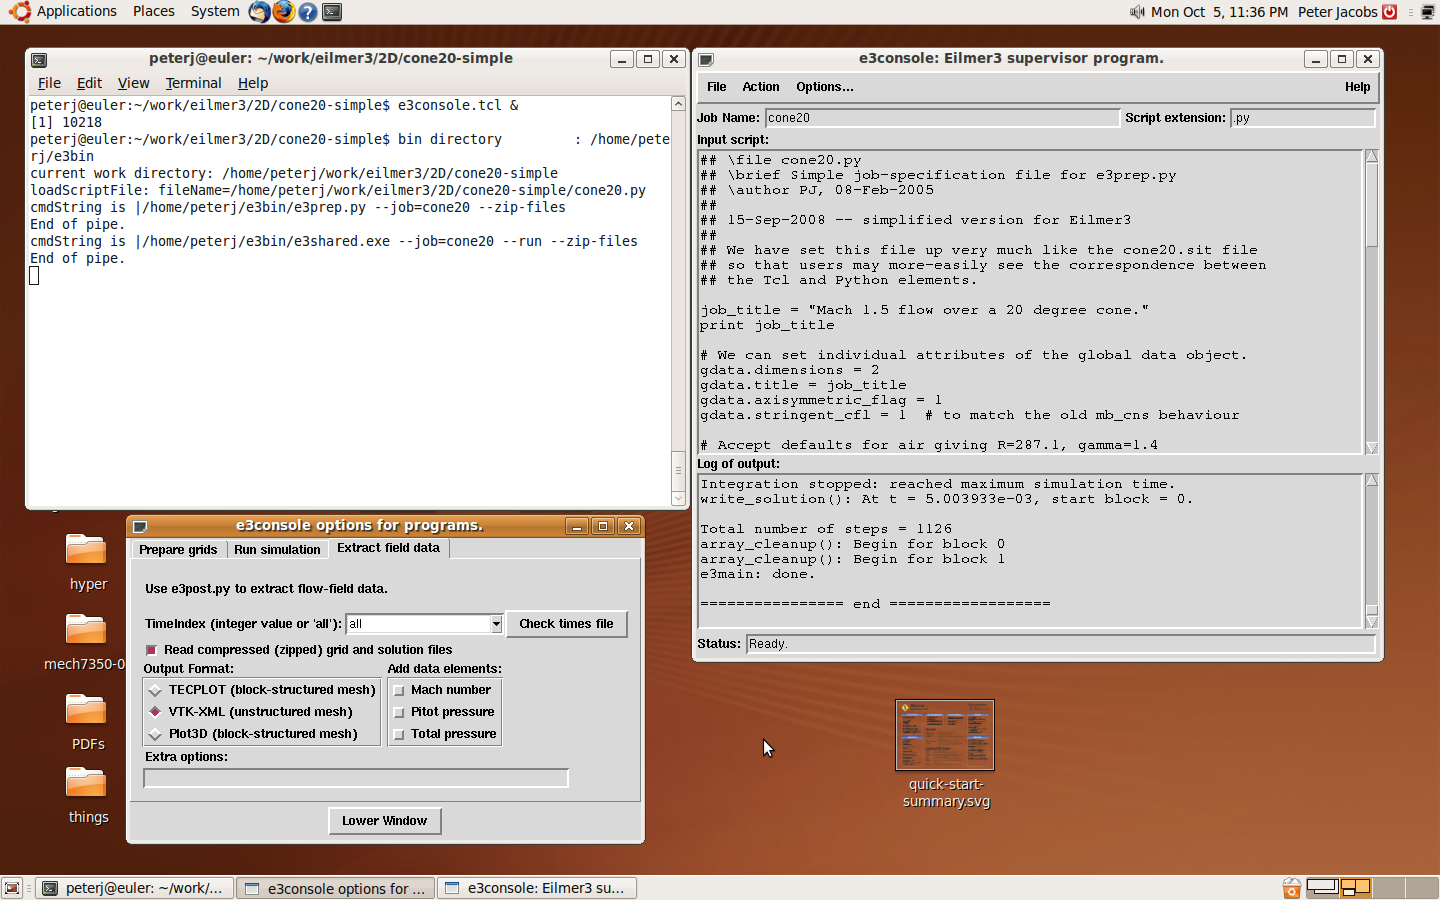
\includegraphics[width=\textwidth]{figs/e3console-screenshot.png}
 \caption{Screen shot of the \texttt{e3console.tcl} GUI running on PJ's workstation.}
 \label{e3console-screenshot-fig}
\end{figure}


\section{Input Script Overview}
Currently, \texttt{e3prep.py}\index{e3prep.py} is implemented as 
a Python program that has a library of classes specialized for constructing
geometric regions and specifying flow conditions.
Because your specification script, \texttt{{\em job}.py}, 
becomes a part of that program when it runs,
it is worth the effort to learn just enough Python to be dangerous.
The web site \url{http://www.python.org} is a good starting point for
learning about the Python programming language, however, Appendix\,\ref{python-notes-sec}
may have enough information to get you started.

\medskip
After doing some initialization, \texttt{e3prep.py} executes your
script file and assembles the geometry and flow specification data
into a form that can be given to the main simulation code
\texttt{e3shared.exe}\index{e3shared.exe}\footnote{The ``shared'' tag indicated that we are
  using the shared-memory version of the code.  
  There is also a distributed-memory version, \texttt{e3mpi.exe}\index{e3mpi.exe},
  based on message passing (MPI) that can be used for running the main simulation.
}.
The advantage of this approach is that you have the full capability of 
the Python interpreter available to you from within your script.
You can perform calculations so that you can parameterize your geometry, 
for example, or you can use Python control structures
to make repetitive definitions much more concise.
Additionally, you may use Python comments and print statements
to add documentation to the script file. 
An input script usually does the following:
\begin{enumerate}
  \item selects gas model
  \item optionally, creates geometric elements to assist in defining the boundary representation of the gas domain
  \item creates blocks within the gas domain and specifies their discretization and, optionally, 
        specifies boundary conditions along some block surfaces (in 3D) or edges (in 2D)
  \item specifies remaining boundary conditions, if any
  \item sets some simulation control parameters
\end{enumerate}
Most examples in this manual do just these things, however, it is possible to do much more.
The example that computes the heat transfer to a sphere (Section\,\ref{sphere-heat-transfer-sec}) uses a top-level Python
script to coordinate a number of simulations with increasingly-refined grids as a crude multigrid simulation.

\medskip
To aid with debugging, it is easy to process part of your input script and
then temporarily put the interpreter into an interactive mode where 
you may type python commands and expressions at the prompt (\texttt{>>>}).
To do so, add the following lines at the appropriate point in your input
script.\\
%
\topbar\\
\texttt{from code import interact}\index{e3prep.py!interactive mode}\\
\texttt{interact('Start interactive mode (Ctrl-D to return)', local=locals())}\\
\bottombar\\
%
Now you can interact with the Python environment and the objects that your
input script has defined so far.
For example, to find out a bit about defining \texttt{Block3D} objects, type:\\
%
\topbar\\
\texttt{>>> help(Block3D)}\\
\bottombar\\
%
To get out of the interactive mode and continue processing the input script,
type \texttt{Control-D} at the prompt.


%------------------------------------------------------------------
\section{Thermochemical model and flow conditions}
\label{thermo-flow-sec}\index{thermochemical models}\index{module!libgas}
%
The thermochemical models are provided by the \texttt{libgas} module.
This is primarily a C++ module but it has a SWIG-generated Python interface so
that its objects and methods can be accessed from the user's input script.

\subsection{10 second version: just tell me how to select perfect air}
Place the following text (which is a function call) in your script \emph{before}
specifying any \texttt{FlowCondition} objects:\\
%
\topbar\\
\texttt{select\_gas\_model(model='ideal gas', species=['air'])}\\ \index{select\_gas\_model}
\bottombar\\
%
If this is the only gas model that interests you for the present, then
proceed to page~\pageref{sec:flow_condition} which discusses the specification
of a \texttt{FlowCondition}.

\subsection{2 minute version: tell me about other simple models}

To select a gas model, the user calls the function
\texttt{select\_gas\_model}.
This function accepts three keyword arguments: \texttt{model},
\texttt{species}, and \texttt{fname}.
In the vast majority of cases, only the first
two keyword arguments will be used.
This function must be called \emph{before} specifying any \texttt{FlowCondition} objects
so that the complete thermodynamic state can be computed.

\medskip
A second example: to select an ideal mixture of nitrogen and oxygen
call:\\
%
\topbar\\
\texttt{select\_gas\_model(model='ideal gas', species=['N2', 'O2'])}\\
\bottombar\\
%
Note that the only difference between selecting a mixture and a single
component gas is the addition of extra species in the species list and the extra computation that
the main simulation program needs to do.

\medskip
In general, the \texttt{model} keyword accepts a string describing
the gas model behaviour.
The available gas models are:
\begin{itemize}
 \item \texttt{'ideal gas'}: a gas with ideal behaviour: modelled as having perfectly elastic collisions
                             and constant specific heats\index{gas model!ideal}
 \item \texttt{'thermally perfect gas'}: a gas with thermally perfect behaviour: modelled as having perfectly
                             elastic collisions but with specific heats that are functions of temperature
                             \index{gas model!thermally perfect}
% \item \texttt{'one temperature gas'}: similar to the 'thermally perfect gas' except that the thermodynamic 
%                             properties are calculated from statistical mechanics rather than the CEA curve 
%                             fits\footnote{Due to the assumption of decoupled thermal modes, the thermodynamic
%                             properties for the 'one temperature gas' model are not as accurate as the CEA curve
%                             fits.  The purpose of the this gas model is to provide a single temperature 
%                             equivalent of the multiple temperature gas models.  For general thermal equilibrium
%                             calculations, users are advised to use the 'thermally perfect gas' model.}, and
%                             transport properties are calculated via collision-integrals.
 \item \texttt{'two temperature gas'}: a thermally perfect gas\footnote{The two temperature gas model is thermally
                             perfect in the sense that the thermodynamic properties are functions
                             of temperature only, however multiple temperatures are defined.} with two independent
                             thermal modes: one temperature $T_\text{tr}$ governs the heavy-particle translation 
                             and rotation modes, and another temperature $T_\text{ve}$ governs the vibration, 
                             electronic and free-electron translation modes.
                             \index{gas model!two temperature}
% \item \texttt{'three temperature gas'}: a thermally perfect gas with three independent thermal modes: the 
%                             temperature $T_\text{tr}$ governs the heavy-particle translation and rotation modes,
%                             $T_\text{v}$ governs the vibration modes and $T_\text{e}$ governs the
%                             electronic and free-electron translation modes.
%                             \index{gas model!three temperature}
% \item \texttt{'four temperature gas'}: a thermally perfect gas with four independent thermal modes: the 
%                             temperature $T_\text{t}$ governs the heavy-particle translation modes, $T_{\text{r}}$
%                             governs the rotation modes, $T_\text{v}$ governs the vibration modes and $T_\text{e}$ 
%                             governs the electronic and free-electron translation modes.
%                             \index{gas model!four temperature}
 \item \texttt{'real gas Bender'}: a gas with real behaviour, such as accurate thermodynamic property evaluation
                            at high density and pressure near the saturation boundary and in the critical region.
                            This model is based on the Bender \textit{p-v-T} relationship.
                             \index{gas model!real gas!Bender}
 \item \texttt{'real gas MBWR'}: a gas with real behaviour, such as accurate thermodynamic property evaluation
                            at high density and pressure near the saturation boundary and in the critical region.
                            This model is based on the MBWR \textit{p-v-T} relationship, which is more accurate
                            than the Bender \textit{p-v-T} relationship.
                             \index{gas model!real gas!MBWR}
 \item \texttt{'real gas REFPROP'}: a gas with real behaviour, such as accurate thermodynamic property evaluation
                            in all single and two phase regions.
                            This model makes use of the REFPROP thermodynamic database and is more accurate than
                            the MBWR gas model.
                             \index{gas model!real gas!REFPROP}
\end{itemize}

The \texttt{species} keyword accepts a list of strings; each string denotes
a species in the mixture.  The order of this list is important: the order of
species in this list corresponds to the order in which the species mass fractions
are specified in other parts of the input.
To get a list of available species, look at the selection of species which are placed
in the \texttt{\$HOME/e3bin/species}\index{species!list of available} area during the install, 
that is, at a command prompt type:

\noindent
\topbar\\
\texttt{> ls \$HOME/e3bin/species}\\
\bottombar\\
%
The names of these files (excluding the \texttt{.lua} extension) correspond to the
names of available species.  The \texttt{defaults.lua} file is not a species name.
Rather, this file provides a set of default values when no other data is available.

\subsection{10 minute version: the detail of gas model configuration}
In the last two examples, the \texttt{select\_gas\_model} function was called using
the two keyword arguments \texttt{model} and \texttt{species}.
Behind the scenes, this function calls an auxiliary set of tools to build
a stand-alone text file which is a configuration file for the gas model.
This configuration file is a Lua-style file: it is read directly by the
C++ code (with embedded Lua interpreter) in order to configure the gas model.
By default, the created configuration file is called \texttt{gas-model.lua}.
This file will sit in your working directory after a successful call to
\texttt{select\_gas\_model} using only the \texttt{model} and \texttt{species} keyword
arguments.
The configuration file contains all the necessary details to completely
specify the gas.
Thus, this file serves as a record of the gas model input parameters used in
your simulation.

\medskip
You are encouraged to open the file \texttt{gas-model.lua} and take a look.
It contains not only the input parameters for the gas model but also references for the
data where possible.
Some amount of effort has been made to design a configuration file that
properly documents the input data.
The use of Lua as the configuration language has aided this effort.

\medskip
Alternatively, the \texttt{select\_gas\_model} function may also be called
with \texttt{fname} as a keyword argument.
This argument, \texttt{fname}, accepts a string which names a Lua-style configuration
file for the gas model.
Thus, if you have a gas model configuration file from a previous simulation, you could
set the gas model with the call:\\
%
\topbar\\
\texttt{select\_gas\_model(fname='gas-model.lua')}\\
\bottombar\\
%
This assumes your configuration file is called \texttt{gas-model.lua} and resides
in the same directory as your main simulation script.\index{gas model!gas-model.lua file}

\medskip
Finally, for certain advanced gas models (such as a gas with multiple vibrational temperatures),
the only means to configure these models is via the preparation of a Lua-style configuration
file by hand.
After building a file by hand (that is, in a text editor), one would use the \texttt{fname} keyword
argument in the call to \texttt{select\_gas\_model} to set the gas model.
The list of gas models which are set by directly creating a configuration file are:
\begin{itemize}
 \item user-defined gas (by specification of callable Lua functions)\index{gas model!user-defined}
 \item an equilibrium gas, based on a look-up table\index{gas model!look-up table}
 % DFP: this model is specified via 'thermally perfect gas'
 % \item a reacting mixture of thermally perfect gases\index{gas model!reacting}
\end{itemize}
Further discussion of gas models which are set by direct creation
and manipulation of a configuration file is given in Appendix~\ref{app:gas-models}.

\subsection{Selecting a simple model and adjusting it}
The simple ideal gas model of air as discussed above has $\gamma = 1.4$.
You can get an air model with $\gamma = 1.3$ by selecting the species
as \texttt{'air13'} or you can adjust the value of $\gamma$ directly
for the ideal gas model.
This can be done from within the Python input script by calling the function 
\texttt{change\_ideal\_gas\_attribute()},\index{gas model!change\_ideal\_gas\_attribute}
and telling it which species, which attribute and what new value to use.
The function actually does a string substitution within the \texttt{gas-model.lua} file
that was generated behind the scenes when the \texttt{select\_gas\_model()} function was called.

\medskip
For an example of use, see the MNM Implosion problem in Section\,\ref{mnm-implosion-sec}.
There, the value of ratio of specific heats is changed with the lines\\
%
\topbar\\
\texttt{gas\_gamma = 5.0/3.0}\\
\texttt{select\_gas\_model(model='ideal gas', species=['air'])}\\
\texttt{change\_ideal\_gas\_attribute('air', 'gamma', gas\_gamma)\\}
\bottombar\\
You might also like to change the gas constant but, since that is not an actual parameter in the 
\texttt{gas-model.lua} file, it needs to be set indirectly, via the molecular mass (in units of kg/mol).\\
\topbar\\
\texttt{Rgas = 300.0}\\
\texttt{MM = R\_u / Rgas}\\
\texttt{change\_ideal\_gas\_attribute('air', 'M', Rgas)\\}
\bottombar\\
Note that \texttt{'M'} is the label for molecular mass in the \texttt{gas-model.lua} file
and \texttt{R\_u} is the universal gas constant made available by the thermochemistry module
to the Python input script.


\subsection{Specifying chemically reacting flow}
\index{chemical reaction!reaction scheme file}
For chemically reacting flow simulations, the following function call is
required:\\
%
\topbar\\
\texttt{set\_reaction\_scheme(config\_file, reacting\_flag=1)}\\
\bottombar\\
where \texttt{config\_file} is a string naming the configuration file for the
chemical reaction scheme.  This configuration file specifies all of the chemical
reactions between the various species and is built by hand by the user.\index{chemical reaction}
By default, the reactions are turned on, however, the user may elect to turn off
chemical reaction updates by setting \texttt{reacting\_flag=0}.

\medskip
An example of a reacting flow simulation is given in Section~\ref{sec:n90}.
The details of building a chemistry input file are provided in Appendix~\ref{app:chem}.

\subsection{Specifying thermal energy exchange mechanisms}
\index{thermal nonequilibrium!energy exchange scheme file}
For flow simulations where the number of thermal modes is greater than one (such as for the 
`two temperature gas' model previously
mentioned), energy exchange mechanisms can be defined that describe the exchange of thermal
energy between modes due to particle collisions.
If such energy exchange mechanisms wish to be modelled, the following function call is
required:\\
%
\topbar\\
\texttt{set\_energy\_exchange\_update(config\_file)}\\
\bottombar\\
where \texttt{config\_file} is a string naming the Lua configuration file for the
energy exchange scheme.  This configuration file specifies all of the energy exchange 
mechanisms between the thermal modes due to thermal processes (i.e. particle collisions) 
and is built by hand by the user.\index{thermal energy exchange}
Thermal energy exchange is automatically turned on when the
\texttt{set\_energy\_exchange\_update(config\_file)} function call is made.

\medskip
An example of a flow simulation with thermal energy exchange is given in
Section~\ref{sec:finite-cyl-sec}.
The details of building a thermal energy exchange input file are provided in 
Appendix~\ref{app:therm-exchange}.

\subsection{Defining flow conditions}
\label{sec:flow_condition}
Because \texttt{Eilmer3} is a flow \textit{simulation} code, initial gas flow conditions
need to be specified throughout the domain.
Also, depending on your model, free-stream inflow boundary conditions 
may need to be specified on appropriate boundary surfaces.
To define such a flow condition in your input script for one or both of these purposes, 
create a \texttt{FlowCondition} object\footnote{The \texttt{FlowCondition} class is
  defined in source file \texttt{e3\_flow.py}} as:
\texttt{
\begin{tabbing}
my\_flow = FlowCondition(\=p=1.0e5, u=0.0, v=0.0, w=0.0, T=[300.0,], \\
                         \>massf=None, label="", tke=0.0, omega=1.0, \\
%                         \>sigma\_T=0.0, sigma\_c=0.0, 
                         \>S=0, add\_to\_list=1)
\end{tabbing}
}\index{FlowCondition}\index{FlowCondition!add\_to\_list parameter}

%
\begin{itemize}
  \item \texttt{p}: pressure in Pa, default value 100\,kPa.
  \item \texttt{u}: $x$-coordinate velocity in m/s, default value 0.0.
  \item \texttt{v}: $y$-coordinate velocity in m/s, default value 0.0.
  \item \texttt{w}: $z$-coordinate velocity in m/s, default value 0.0.
  \item \texttt{T}: list of temperatures in degrees K, default value [300.0,].
    For gas models with multimodal energies, these are the corresponding temperatures.
    For a gas model with only one internal energy mode, you may specify a scalar value
    for temperature.
  \item \texttt{massf}: mass fractions of the component species.
    These may be provided in a number of ways:
    \begin{itemize}
      \item[(a)] full list of floats. The length of the list of mass fractions 
         must match the number of species in the previously selected gas model.
      \item[(b)] single float or integer that gets used as the first element,
         the rest being set 0.0
      \item[(c)] dictionary of species names with mass fraction values,
         the remainder being set 0.0.  See the example in Section\,\ref{sec:MoleFractions}.
      \item[(d)] None provided, results in the first element being 1.0
         and the rest 0.0
    \end{itemize}
    Note that the mass fractions supplied must sum to 1.0 (within a tolerance of $1.0 \times 10^{-6}$.
  \item \texttt{label}: (optional) text label for the FlowCondition object.
  \item \texttt{tke}: turbulent kinetic energy per unit mass in m$^2$/s$^2$ or
    J/kg, default value 0.0.
  \item \texttt{omega}: turbulence vorticity in 1/s, default value 1.0.
  \item \texttt{mu\_t}: turbulence viscosity in Pa.s, default value 0.0.
  \item \texttt{k\_t}: turbulence thermal conductivity, default value 0.0.
     This might be conveniently computed as $C_p \mu_t / Pr_t$.
%  \item \texttt{sigma\_T}: variance of temperature variations, default value 0.0.
%  \item \texttt{sigma\_c}: variance of species concentrations, default value 0.0.
  \item \texttt{S}: integer shock indicator value, default value 0.
    A value of 1 indicates the presence of a shock through the cell.
  \item \texttt{add\_to\_list}: flag to indicate that this FlowCondition object 
    should be added to the flowList.  Sometimes we don't want
    to accumulate objects in this list, for example, when using
    many FlowCondition objects in a user-defined flow evaluation function.
    default value 1.
\end{itemize}

\medskip
Simulations involving nonequilibrium chemistry require and extra input file
describing the participating gas species and their reactions.
Preparation of this file is described in Appendix\,\ref{app:chem}.

\subsection{Using flow conditions from other simulations}
\label{sec:ExistingSolution}
%
There are occasions where you might like to use flow data from an old simulation
as initial conditions for some or all of your blocks in your new simulation.
A typical use case is to restart a simulation with a finer, or otherwise changed, mesh.
For this, you may pick up the old simulation data using:\\
\index{ExistingSolution}
\texttt{
\begin{tabbing}
old\_flow = ExistingSolution(\=rootName, solutionWorkDir, nblock, tindx, \\
                             \>dimensions=2, assume\_same\_grid=0, zipFiles=1, \\
                             \>add\_velocity=Vector(0.0,0.0,0.0))\\
\end{tabbing}
}\index{ExistingSolution}
where the arguments and their possible values are:
\begin{itemize}
  \item \texttt{rootName}: job name that will be used to build file names
  \item \texttt{solutionWorkDir}: the directory where we'll find our existing solution files.
  \item \texttt{nblock}: number of blocks in the existing solution data set
  \item \texttt{tindx}: the time index to select 0..9999.
            Do not specify with leading zeros because the Python interpreter
            will assume that you want to count the time index in octal.
  \item \texttt{dimensions}: number of spatial dimensions for the existing solution
  \item \texttt{assume\_same\_grid}: decide how to locate corresponding cells
     \begin{itemize}
        \item[\texttt{0}]: searches for corresponding cells. This steps through each cell and
		searches for closest corresponding cell centre in the old solution and inserts
		the flow data.
                As Rainer found, this can be agonisingly slow for large grids.\index{Kirchhartz}
        \item[\texttt{1}]: omits the search for the corresponding cell.
                Definitely the option for the impatient. This assumes the same grid for the old and
		new solution and inserts flow data based on the i and j cell references.
     \end{itemize}
   \item \texttt{zipFiles}: to use gzipped files (1), or not (0)
   \item \texttt{add\_velocity}: value to be added to each cell's velocity,
       for changing frame of reference.
\end{itemize}
The process of writing the data into each cell of the new grid uses a fairly naive search for the 
nearest cell in the existing solution.
Although it is robust, the search is extremely slow and the preparation of sew grids has been known
to take hours of CPU time.
If the new simulation is a continuation of the old simulation, it may be appropriate to set
\texttt{gdata.t0} to a nonzero value.  See Section\,\ref{sec:sim-control-parameters}.

\subsection{Using mole fractions and species dictionaries}
\label{sec:MoleFractions}
%
When simulating flows with mixes of gas species, it may be more convenient to specify the gas mix
via mole fractions rather than mass fractions and via a dictionary rather than a list.
With large numbers of species in the gas model, specification of the mix via dictionary is far easier to
read and check than when using a list of numerical values. 

\medskip
There are a number of functions attached to the \texttt{Gas\_model} object that make the
conversion to a list of mass fractions easy.
Here is an extract from Umar's standing-shock script showing the creation of a fairly complex gas mix
using a dictionary of mole fractions.

\medskip\noindent\topbar\\
{\small %\scriptsize
\begin{verbatim}
select_gas_model(model='thermally perfect gas', 
                 species=['O', 'N', 'N2', 'O2', 'NO', 'N_plus', 'O_plus', 'N2_plus',
                          'O2_plus', 'NO_plus', 'e_minus', 'Ar', 'Ar_plus'])
set_reaction_scheme("gupta_etal_air_reactions.lua", reacting_flag=1)
gmodel = get_gas_model_ptr()

# Pre-shock gas: mass fractions for an ideal air mixture.
mi = {'N2':0.769, 'O2':0.231}
# Post-shock: mole fractions from a CEA calculation.
X = {'O':1.6936e-1, 'N':5.9784e-1, 'N2':6.9757e-5, 'O2':4.7543e-8, 'NO':2.5654e-3, 
     'N_plus':9.6331e-2, 'O_plus':1.7562e-2, 'N2_plus':7.7688e-6, 'O2_plus':5.0837e-8, 
     'NO_plus':1.4459e-5, 'e_minus':1.1436e-1, 'Ar':4.0026e-3, 'Ar_plus':4.4835e-4}

initial = FlowCondition(p=2700.0, u=0.0, v=0.0, T=300.0, massf=mi)
inflow  = FlowCondition(p=4464.0, u=10284.0, v=0.0, T=10140.42,
                        massf=gmodel.to_massf(X))
\end{verbatim}
}
\noindent\bottombar


%-------------------------------------------------------------------
\section{Boundary representation of the gas domain}
%
Most of the effort required to set up a simulation goes into defining the
``body-fitted'' grid of finite-volume cells that completely fills the flow
domain.
The top-level geometry description given to the grid generator is in terms of
``patches'' for 2D flow and ``parametric volumes'' for 3D flow.
These are regions of space that may be traversed by
a set of parametric coordinates $0 \le r < 1$, $0 \le s < 1$ (in 2D) and 
with the third parameter $0 \le t < 1$ in 3D.
These patches or volumes can be imported as VTK structured grids or they can be
constructed as a ``boundary representation'' from lower-dimensional 
geometric entities such as paths and points.

\subsection{Geometric elements}
%
The most fundamental class of geometric object is the \texttt{Vector}\index{geometric element!Vector} (or
\texttt{Vector3}\index{geometric element!Vector3} as it is defined in the C++ module \texttt{libgeom2}\index{module!libgeom2}).
A \texttt{Vector} represents a point in 3D space and has the usual behaviour 
of a geometric vector (as opposed to the \texttt{vector} collection class in
C++).
See, for example, the postprocessing program in the \texttt{simple\_ramp}
simulation (Section\,\ref{simple-ramp-post-files}).
If you want a point to be rendered with a label, you can define it as a
\texttt{Node}.
Examples of use include: $a$ = \texttt{Vector}($x$, $y$, $z$) and
$b$ = \texttt{Node}($x$, $y$, $z$, \texttt{label='B'}).\index{geometric element!Node}

\medskip
It is also possible to 'get' and 'set' values within a geometric element. For example to
create a node, extract the x value of that node, to change the y value or to use
the geometry values for a new node could be done as follows.\\
\topbar\\
\texttt{a = Node(0.5,0.8,label='Node a')}\\
\texttt{x-value = a.x}\\
\texttt{a.y = 0.6}\\
\texttt{b = Node(a.x, a.y+0.2,label='Node b')}\\
\bottombar\\

\medskip
If you look into the file \texttt{cfcfd3/lib/geometry2/source/geom.hh}, you will see that
the \texttt{Vector3} objects support the usual vector operations of addition, subtraction and the like.
Also, you can \texttt{clone} and transform a point.
For example, to create a point and its mirror image in the (x,z)-plane, you could use\\
\topbar\\
\texttt{a = Vector(0.5, 0.6)}\\
\texttt{b = a.clone().mirror\_image(Vector(0.0,0.0), Vector(0.0,1.0)}\\
\bottombar\\
 
\subsubsection{Paths}
%
The next level of dimensionality is the \texttt{Path} class\index{geometric element!Path}.
A path object is a parametric curve in space, 
along which points can be specified via the single parameter $0 \le t < 1$.
Types of paths that are available include:
\begin{itemize}
\item \texttt{Line}($a$, $b$): a straight line between points $a$ and $b$.\index{geometric element!Line}
\item \texttt{Arc}($a$, $b$, $c$): a circular arc from $a$ to $b$ around centre,
  $c$.\index{geometric element!Arc}
  Be careful that you don't try to make an \texttt{Arc} with included angle of 180$^o$ or greater.
  For such a situation, create two circular arcs and join as a \texttt{Polyline} path.
\item \texttt{Arc3}($a$, $b$, $c$): a circular arc from $a$ through $b$ to $c$.
  All three points lie on the arc.\index{geometric element!Arc3}
\item \texttt{Helix}($a_0$, $a_1$, $x_{local}$, $r_0$, $r_1$, $d\theta$): a helical path
  about a specified axis, start and end radii and angle through which the path extends.\index{geometric element!Helix}
\item \texttt{Helix}($p_0$, $p_1$, $a_0$, $a_1$): a helical path through specified points
  and about a specified axis.
  Internally, it is stored as the helical path described above.
\item \texttt{Bezier}([$b_0, b_1, ..., b_n$]): a Bezier curve from $b_0$ to
  $b_n$.\index{geometric element!Bezier}
\item \texttt{Nurbs}($CP[.]$, $w[.]$,$degree$, $U[.]$): nonuniform rational B-spline with
  control points vector $CP[.]$, weights vector $w[.]$, and knot vector $U[.]$.\index{geometric element!Nurbs}
\item \texttt{Polyline}([$p_0, p_1, ..., p_n$]): a composite path made up of 
  the segments $p_0$, through $p_n$.\index{geometric element!Polyline}
  The individual segments are reparameterised, based on arc length, so that
  the composite curve parameter is $0 \le t < 1$.
\item \texttt{Polyline2}(*args): a composite path constructed from path elements and/or \texttt{Vector} points.
  If there are gaps between the elements and points, 
  they will be filled with \texttt{Line} segments.\index{geometric element!Polyline2}
\item \texttt{Spline}([$b_0, b_1, ..., b_n$]): a cubic spline from $b0$ through
  $b1$, to $bn$.\index{geometric element!Spline}
  A \texttt{Spline} is actually a specialized \texttt{Polyline}.
\item \texttt{Spline2}(filename): a spline constructed from a file containing $x(,y(,z))$ coordinates
  of the interpolation points, one point per line.
  If the $y$ or $z$ values are missing, they are assumed to be zero.\index{geometric element!Spline2}
\item \texttt{PathOnSurface}($S$, $f_r$, $f_s$): a path on the
  ParametricSurface $S(r,s)$, defined by the univariate functions 
  $r=f_r(t)$ and $s=f_s(t)$.\index{geometric element!PathOnSurface}
\item \texttt{PolarPath}($P$, $H$): A path in 3D space made from another path, $P$,
  such that the neutral plane at height $H$ is wrapped around a cylinder aligned with
  the x-axis.\index{geometric element!PolarPath}
\item \texttt{PyFunctionPath}($f$): a path defined by the user-supplied Python function, $f(t)$.
  The user function returns a tuple of three values representing the point in space 
  for parameter value $t$.\index{geometric element!PyFunctionPath}
\end{itemize}

Most \texttt{Path} objects (except \texttt{PyFunctionPath}) support the transformation methods
\texttt{translate(displacement)}, 
\texttt{reverse()}, 
\texttt{mirror\_image(point, normal)} and \\
\texttt{rotate\_about\_zaxis(radians)}.
Look in the source code files \texttt{gpath.hh} and \texttt{gpath.cxx} for details.
These may be found in the directory \texttt{cfcfd3/lib/geometry2/source/}.

\subsubsection{Surfaces}
%
The \texttt{ParametricSurface}\index{geometric element!ParametricSurface} class 
represents two-dimensional objects which can be constructed from \texttt{Path} objects.
Examples are:
\begin{itemize}
\item \texttt{CoonsPatch}($p_S, p_N, p_W, p_E$): a transfinite interpolated
  surface between the four paths.\index{geometric element!CoonsPatch}
  It is expected that the paths join at the corners of the patch, such that
  $p_S(0) = p_W(0) = p00$, $p_S(1) = p_E(0) = p10$, $p_N(0) = p_W(1) = p01$ and $p_N(1) =  p_E(1) = p11$.
  See the left part of Figure\,\ref{block2d-defn-fig} for the layout of this surface.
  Note that, although we are using subscripts aligned with the BOTTOM and TOP
  surfaces in this description, the same order is used for the other surfaces
  when the local surface parametric directions are aligned with the relevant index
  directions.
  See the debugging cube in Appendix\,\ref{cube-development}.
  Be aware that the order of the supplied paths for each surface is (SOUTH, NORTH, WEST, EAST),
  which is different to the order accepted by the \texttt{make\_patch()} function 
  that is used to make two-dimensional grids in the following section.  
  Finally, it is important to be careful with the orientation of the \texttt{Path}
  elements that form the patch boundaries.
  The NORTH and SOUTH boundaries progress WEST to EAST as shown in Figure\,\ref{block2d-defn-fig}
  (in the following section).
  The WEST and EAST boundaries progress SOUTH to NORTH.
  If the \texttt{e3prep.py} program complains that the corners of your patch are ``open'',
  that may be a symptom of having one, or more, of your bounding paths having incorrect orientation.
\item \texttt{AOPatch}($p_S, p_N, p_W, p_E$): an interpolated surface \index{geometric element!AOPatch}
  that tries to keep the grid orthogonal near the edges and 
  also tries to keep equal areas across the surface.
\item \texttt{MeshPatch}: a surface defined over a structured mesh of
  quadrilateral facets.\index{geometric element!MeshPatch}
  This might be useful for generating new grids from files imported from
  an external grid generator.
\item \texttt{TrianglePatch}: a surface defined over an unstructured mesh of
  triangular facets.\index{geometric element!TrianglePatch}
  When the surface is really too complex to describe as a simpler form,
  this type of surface can conform (approximately) to just about anything.
\item \texttt{BezierPatch}: a surface defined over a tensor product of Bezier curves.\index{geometric element!BezierPatch} 
\item \texttt{RevolvedSurface}($p$): a surface defined by rotating Path $p$
  about the $x$-axis.\index{geometric element!RevolvedSurface}
  When calling the \texttt{eval(r,s)} method for this surface, 
  the first parameter, \texttt{r}, is along the path and the second parameter, 
  \texttt{s}, is the angle in the ($y,z$)-plane.
\item \texttt{MappedSurface}($S_{query}$, $S_{true}$)\index{geometric element!MappedSurface}: points on the
  query surface are projected onto the true surface.
  The final surface is a subset of the true surface.
  Usually the query surface is something simple like a \texttt{CoonsPatch}
  that is close to the shape of the desired grid and
  the true surface could be constructed as a \texttt{RevolvedSurface} which is
  a bit difficult to grid regularly.
\item \texttt{PolarSurface}($S$, $H$): A surface in 3D space made from another surface, $S$,
  such that the neutral plane at height $H$ is wrapped around a cylinder aligned with
  the x-axis.\index{geometric element!PolarSurface}
\item \texttt{SurfaceThruVolume}($V$,$f_r$,$f_s$,$f_t$)\index{geometric element!SurfaceThruVolume}: a surface through the
  ParametricVolume $V(r,s,t)$, defined by the univariate functions 
  $r=f_r(t)$, $s=f_s(t)$ and $t=f_t(t)$.
\item \texttt{NurbsSurface}\index{geometric element!NurbsSurface}: a surface defined as the tensor product of non-uniform rational B-splines.
\item \texttt{PyFunctionSurface}($f$)\index{geometric element!PyFunctionSurface}: a surface defined by the user-supplied Python function, $f(r,s)$.
  The user function returns a tuple of three values representing the point in 3D space 
  for parameter values $r$ and $s$.
  If you are trying to build a 2D simulation, just return the z-coordinate as zero.
\end{itemize} 

Except for \texttt{PyFunctionSurface}, most of the surface objects can be cloned and transformed
with \texttt{translate}, \texttt{mirror\_image} and \texttt{rotate\_about\_zaxis} methods.
Again, see the source code for details.


\subsubsection{Volumes}
%
Finally, in its most general form, a 
\texttt{ParametricVolume}($S_N, S_E, S_S, S_W, S_T, S_B$) \index{geometric element!ParametricVolume}
can be constructed from
a set of six parametric surfaces to form a body-fitted hexahedral volume.
More restricted forms of a volume can be constructed as
\begin{itemize}
\item \texttt{WireFrameVolume}($p_{01}, p_{12}, p_{32}, p_{03}, p_{45},
  p_{56}, p_{76}, p_{47}, p_{04}, p_{15}, p_{26}, p_{37}$): \index{geometric element!WireFrameVolume} is defined by its
  12 edges (paths).
  Note the implied directions in the subscripts.
  The subscripts correspond to the labelled points in Figure\,\ref{block-defn-fig}.
\item \texttt{WireFrameVolume}($surf, p$): consists of a surface $surf$
  extruded along path $p$.
  The extrusion is actually done be forming a set of 6 surfaces by copying the
  original surface and then constructing four \texttt{CoonsPatch} surfaces
  between them. 
\item \texttt{SimpleBoxVolume}($p_0, p_1, p_2, p_3, p_4, p_5, p_6, p_7$): \index{geometric element!SimpleBoxVolume}
  consists of a straight-edged hexahedral box
  defined by its 8 corner points (as shown in Figure\,\ref{block-defn-fig}).
\item \texttt{MeshVolume}\index{geometric element!MeshVolume}: consists of a \texttt{ParametricVolume}
  interpolated in an existing mesh.
  This mesh may be specified as an array of points or it may be read in from a
  VTK file.
\end{itemize}
There is an alternative approach to defining the ParametricVolume via a user-supplied
Python function as
\begin{itemize}
 \item \texttt{PyFunctionVolume}($f$)\index{geometric element!PyFunctionVolume}: a volume defined by the user-supplied Python function, $f(r,s,t)$.
  The user function returns a tuple of three values representing the point in 3D space 
  for parameter values $r$, $s$ and $t$.
\end{itemize}

Again, transform methods such as \texttt{translate} and \texttt{rotate\_about\_zaxis} may help in 
reducing the amount of user input script required to build complex regions out of multiple \texttt{ParametricVolume}
objects.

%------------------------------------------------------------------
\subsection{Two-dimensional grids}\index{grid!2D}
%
The grid defining the discretized gas domain is block structured. 
In 2D, each block is a patch bounded by 4 edges (NORTH, EAST, SOUTH and WEST) such that
we are looking at a plan-view of the flow domain as shown in Fig.\,\ref{block2d-defn-fig}.

\begin{figure}[htbp]
\mbox{
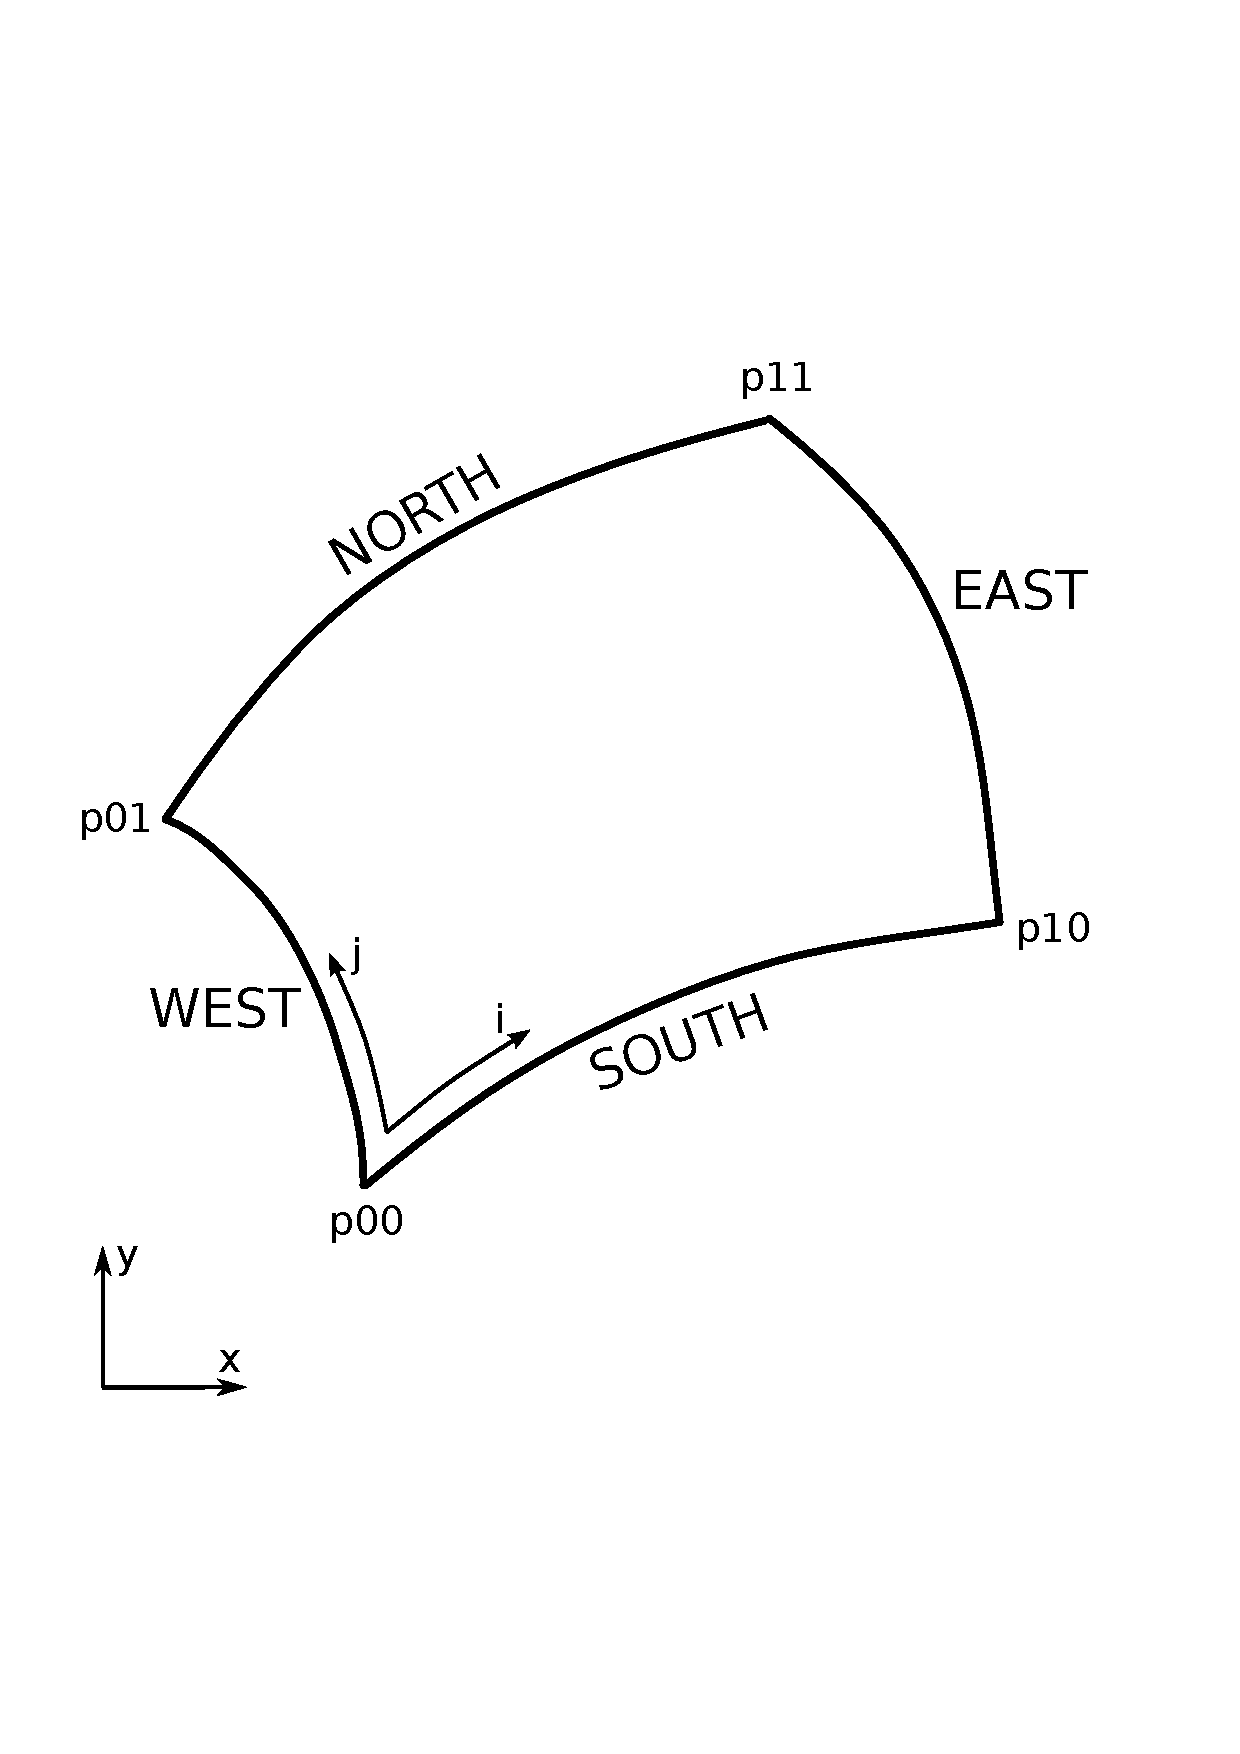
\includegraphics[width=0.5\textwidth,viewport=34 102 524 671,clip=true]{figs/block2d-defn.pdf}
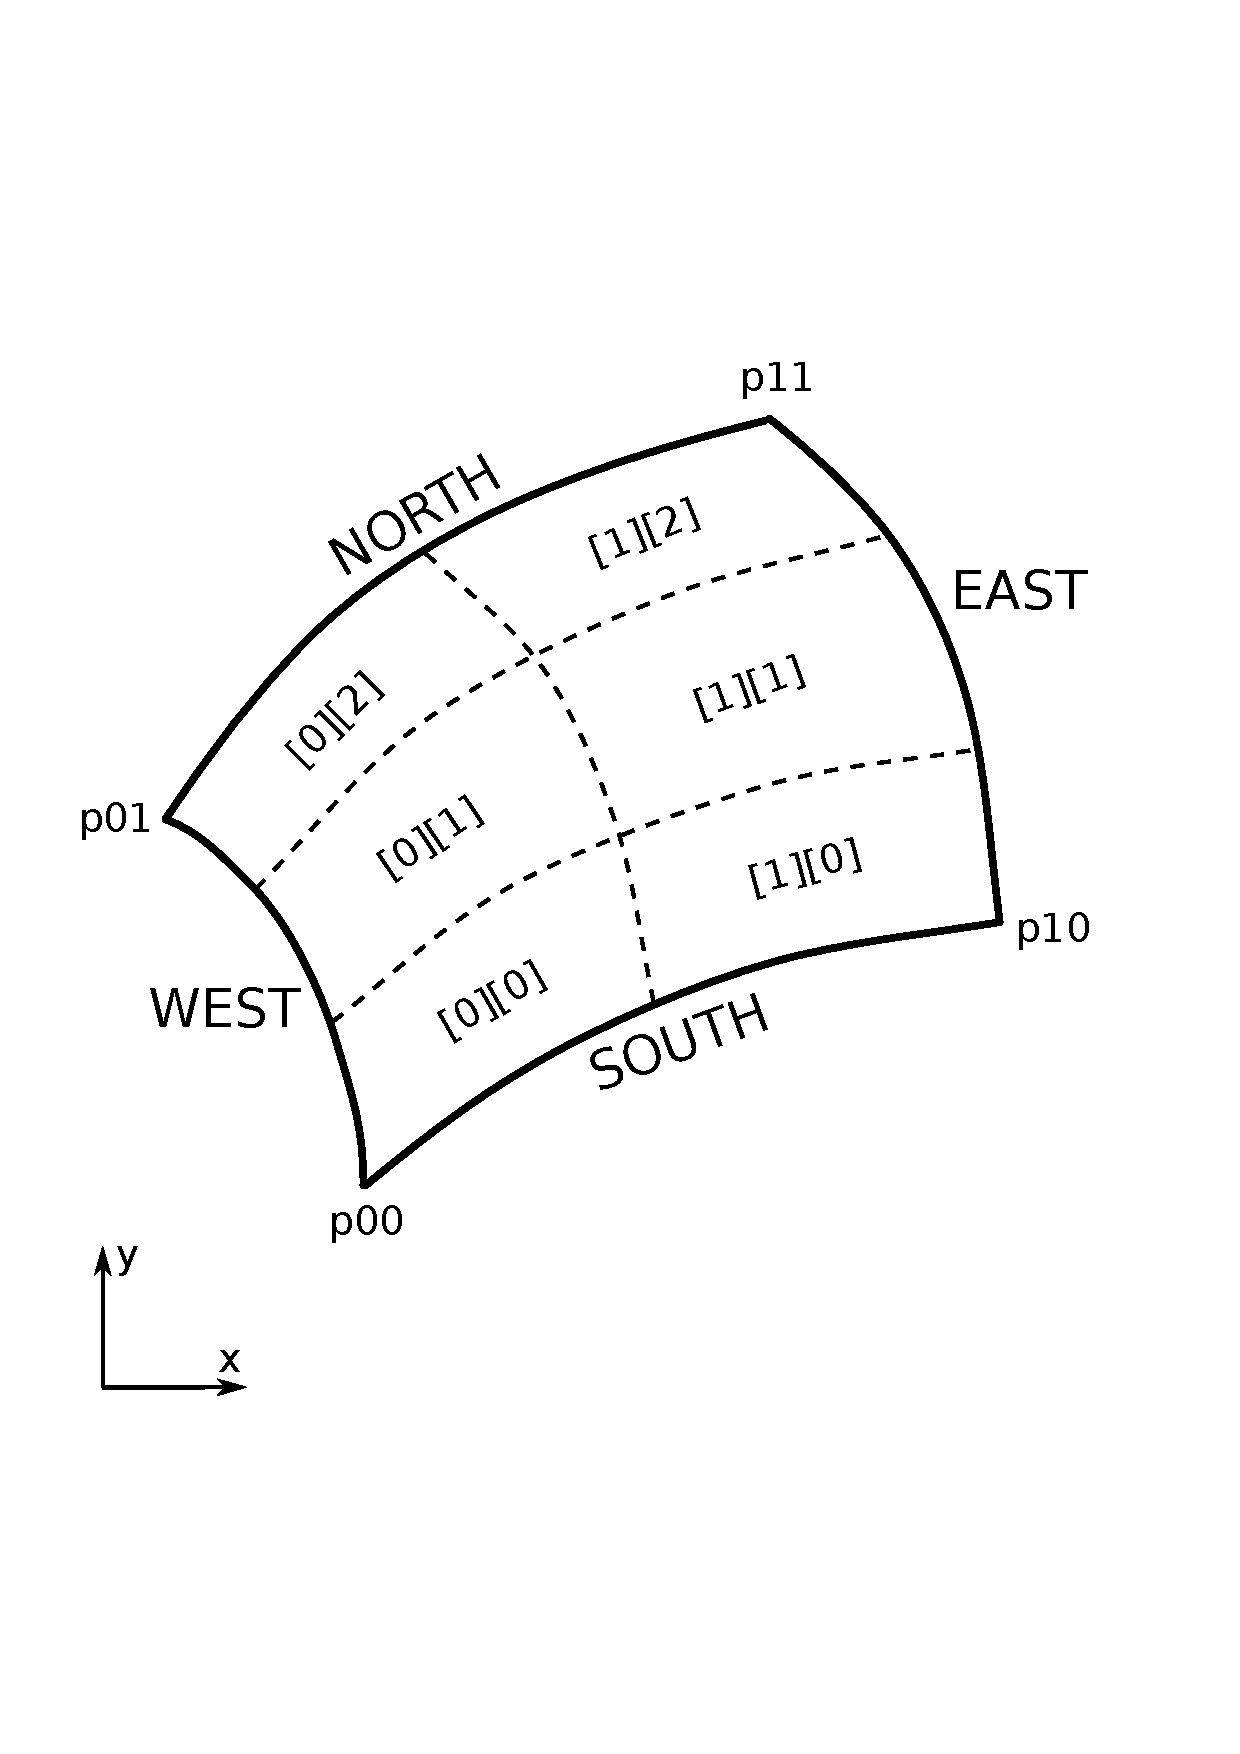
\includegraphics[width=0.5\textwidth,viewport=34 102 524 671,clip=true]{figs/superblock2d-defn.pdf}
}
\caption{A two-dimensional patch containing the structured mesh for a Block2D object (left)
    and a collection of sub-blocks defined via a SuperBlock2D or MultiBlock2D constructor (right).
    The orientations of the bounding paths are important:  
    WEST and EAST paths progress from SOUTH to NORTH;
    SOUTH and NORTH paths progress from WEST to EAST.}
\label{block2d-defn-fig}
\end{figure}

\medskip
To define a block in your input script for a 2D simulation, create a \texttt{Block2D} object as:
\texttt{
\begin{tabbing}
my\_2d\_block = Block2D(\=psurf=None, grid=None, \\
                        \>import\_grid\_file\_name=None, nni=2, nnj=2, \\
                        \>cf\_list=[None,]*4, bc\_list=[SlipWallBC(),]*4, \\
                        \>fill\_condition=None, hcell\_list=[], \\
                        \>xforce\_list=[0,]*4, label="", active=1)
\end{tabbing}\index{block!Block2D}
}
%
\noindent
where the assignment to the name \texttt{my\_2d\_block} allows easy referencing of
the block at later times, say, for adding boundary conditions.
The names of the actual arguments given above match the actual arguments in
the \texttt{e3prep.py} program and these represent\footnote{The
  definitive source is, of course, the \texttt{Block2D} class definition in 
  \texttt{e3\_block.py}\index{module!e3\_block.py}. }:
\begin{itemize}
\item \texttt{psurf}: a region of 2D space bounded by 4 edges.
    This region is often constructed from 4 geometric paths via a call to
    \texttt{make\_patch(north, east, south, west, grid\_type)}\index{make\_patch} where the
    default value for \texttt{grid\_type} is ``TFI'' \textit{i.e.} transfinite interpolation
    or Coons' patch.\index{grid!TFI}\index{grid!transfinite interpolation}
    Another possible form of grid is ``AO'', the area-orthogonality grid.\index{grid!AO}\index{grid!area orthogonality}
    This is the usual way of specifying the flow domain, which will be discretized 
    using \texttt{nni, nnj, and cf\_list}.
    Note that all geometric elements should have zero values for their z-components when
    doing a 2D flow simulation.
    Since most constructors will have a default value of zero for the z-component, this
    detail can usually be ignored.
\item \texttt{grid}: a \texttt{StructuredGrid} object may be supplied (defaults to None). 
\item \texttt{import\_grid\_file\_name}\index{import\_grid\_file\_name} defaults to None.
  If a name is supplied, this file is read to obtain the grid directly.
  The assumed file format in the legacy (ASCII) VTK format for a structured grid.
\item \texttt{nni} is the number of finite-volume cells in the $i$-index
  direction. See the left part of Figure\,\ref{block2d-defn-fig} for the orientation of the index.
  Note that, when placing one block against another, the blocks must conform in
  \begin{itemize}
    \item the number of cells along corresponding edges
    \item the clustering of those cells along the edges
    \item the path defining the corresponding edges.
  \end{itemize}
  The minimum number of cells is 2, because of the way that the cell-interface values are 
  reconstructed from cell-centred data.
\item \texttt{nnj} is the number of finite-volume cells in the $j$-index direction.
\item \texttt{cf\_list} \label{cflist-item} is an optional list of 4 \texttt{UnivariateFunction} objects
  that specify a (possibly) nonuniform distribution of cells along each particular edge.
  \index{clustering!See univariate function}
  For each object, there is an \texttt{eval(t)} method which returns a transformed (new) value of $t$.
  The options available are:
  \begin{itemize}
    \item \texttt{LinearFunction(m, c)}\index{univariate function!LinearFunction}
      where $t_{new} = m \times t_{old} + c$.
    \item \texttt{LinearFunction2(y0, y1)}\index{univariate function!LinearFunction2}
      where $t_{new} = y0 \times (1-t_{old}) + y1 \times t_{old}$.
    \item \texttt{RobertsClusterFunction(end0, end1, beta)}\index{univariate function!RobertsClusterFunction}
      where the \texttt{end0, end1} integer flags indicate which end (possibly both) we wish to cluster toward.
      The value of \texttt{beta} $> 1.0$ specifies the strength of the clustering, with the clustering
      being stronger for smaller values of \texttt{beta}.
      For example, a value of 1.3 would be relatively weak clustering while a value of 1.01 is quite strong
      clustering.
    \item \texttt{ValliammaiFunction(dL0, dL1, L, n)}\index{univariate function!ValliammaiFunction}
      See Adriaan's source code for definitions.
  \end{itemize}
  See the files \texttt{lib/nm/source/fobject.cxx} and \texttt{lib/nm/source/fobject.hh} for details.
  The order of appearance of boundaries in the list is NORTH, EAST, SOUTH and WEST.
  Note that a full list of 4 items is required.
  If you don't want to specify one (or more) of the items in the list, specify \texttt{None} as that item.
\item \texttt{bc\_list} is an optional list of BoundaryCondition objects.\footnote{Note that, 
  when creating these objects in the Python input script, the Python language requires the parentheses
  even for the cases where no arguments, such as \texttt{Twall}, are required. }
  Available boundary conditions are:\index{boundary conditions!list of available}
  \begin{itemize}\index{boundary conditions}
    \item \texttt{AdjacentBC()}\index{boundary conditions!AdjacentBC} for cases where one block interfaces with another.
    \item \texttt{SupInBC(inflow\_condition, label='')}\index{boundary conditions!SupInBC} where we want to specify the inflow condition
      that gets copies into the ghost cells each time step.
      The optional \texttt{label} has an empty default value but may be used to group boundary surfaces symbolically
      in the postprocessing stage.
      Paul Petrie-Repar has made use of these labels in his \texttt{CGNS} postprocessing program.
    \item \texttt{ExtrapolateOutBC(sponge\_flag=0, label='')}\index{boundary conditions!ExtrapolateOutBC} where we want a (mostly supersonic) outflow
      condition.
      Flow data is effectively copied from just inside the boundary to the ghost cells
      just outside the boundary, every time step.
      In subsonic flow, this can lead to unphysical bahaviour.
    \item \texttt{SlipWallBC(label='')}\index{boundary conditions!SlipWallBC} where we want a solid wall with no viscous effects.
      This is the default boundary condition where no other condition is specified.
    \item \texttt{AdiabaticBC(label='')}\index{boundary conditions!AdiabaticBC} where we want viscous effects to impose no-slip at the wall
      but where there is no heat transfer.
    \item \texttt{FixedTBC(Twall, label='')}\index{boundary conditions!FixedTBC} where we want viscous effects to impose a no-slip velocity 
      condition and a fixed wall temperature.
    \item \texttt{SubsonicInBC(stagnation\_condition, label='')}\index{boundary conditions!SubsonicInBC} where the flow is assumed subsonic and
      we specify the stagnation pressure and temperature, but take the velocity from just inside
      the boundary.
    \item \texttt{TransientUniBC(filename, label='')}\index{boundary conditions!TransientUniBC} where we want to specify the time-history of
      the inflow condition.
    \item \texttt{StaticProfileBC(filename, label='')}\index{boundary conditions!StaticProfileBC} where we want to apply a steady-state inflow
       which may vary in space.
    \item \texttt{FixedPOutBC(Pout, label='')}\index{boundary conditions!FixedPOutBC} is like \texttt{ExtrapolateOutBC()} but with a specified 
      back pressure.
      This can be analogous to a vacuum pump that removes gas at the boundary to maintain
      a fixed pressure in the ghost cells.
    \item \texttt{UserDefinedBC(filename, is\_wall=0, use\_udf\_flux=0, label='')}\index{boundary conditions!UserDefinedBC}: 
       allows the user to define the ghost-cell flow properties and/or interface fluxes at run time.
       This is done via a set of functions defined by the user, and written in the Lua
       programming language.
       These functions are provided in the file given by \texttt{filename}.
       The flag \texttt{is\_wall} indicates whether the boundary is to be considered
       a wall for the application of turbulence-model fudges and the like (default 0).
       The flag \texttt{use\_udf\_flux} indicates whether the user is supplying
       the fluxes at the boundary interfaces (default 0).  
       If not, the internal flux calculator is used together with the supplied ghost-cell data.
       This boundary condition is the Jack of all trades and master of none.
       It can be used to emulate any of the other boundary conditions and then build
       variations, however, it is going to cost quite a lot in computational time.
       See Appendix\,\ref{udf-sec} for the details of setting up this boundary condition.
    \item \texttt{AdjacentPlusUDFBC(other\_block, other\_face, orientation, filename, \\is\_wall=0, use\_udf\_flux=0, label='')}\index{boundary conditions!AdjacentPlusUDFBC}: 
       is a combination of the \texttt{AdjacentBC} and \texttt{UserDefinedBC}.
       At each time step, the flow data is first exchanged, as per the usual
       \texttt{AdjacentBC}.  Then the user-defined functions are applied.
       This is one way of getting fancy boundary conditions, such as slowly-opening diaphragms,
       into the simulation.
  \end{itemize}
  These boundary conditions may also be set, one at a time, as described in the 
  Section\,\ref{setting-boundary-conditions-sec}.
\item \texttt{fill\_condition} is the \texttt{FlowCondition} object with which to
  define the initial flow state within the volume.
  See Section\,\ref{thermo-flow-sec} for defining a suitable flow condition.
  You may alternatively provide a Python function that supplies the flow properties as
  a function of position or you may use an \texttt{ExistingSolution()} object.
\item \texttt{hcell\_list} is a list of ($i,j$)-tuples specifying which
  cells should be monitored at simulation time.
  Data from the specified cells will be written to a ``history'' file for the
  block and may be used at the postprocessing stage to provide flow data as if
  there was a sensor located in the cell.
\item \texttt{xforce\_list}\index{xforce\_list} is an optional list of zeros/ones that indicate if we
  want the force to be calculated for each of the four edges and written to the 
  \texttt{e3shared.log} log file.
  See the notes in the 20$^o$ cone test case (Section\,\ref{cone20-simple-sec}) for an
  example of how to extract this data from the log file. 
\item \texttt{label} is an optional text label for the block.  This label
  will be embedded in the block definition and some of the postprocessing
  programs may use it.
  For example, the \texttt{e3cgns.py} postprocessing program uses labels to group block boundaries symbolically.
\end{itemize}
Note that, when lists of items are provided for the four boundaries,
the order of the boundaries is NORTH, EAST, SOUTH and WEST.
 

\medskip
When defining large domains and running simulations of a parallel computer, 
it may be convenient to define many Block2D objects with one call.
The first of two constructors for this situation is
\texttt{
\begin{tabbing}
my\_block\_list = SuperBlock2D(\=psurf=None, nni=2, nnj=2, nbi=1, nbj=1, \\
                               \>cf\_list=[None,]*4, bc\_list=[SlipWallBC(),]*4, \\
                               \>fill\_condition=None, hcell\_list=[], label="sblk")
\end{tabbing}\index{block!SuperBlock2D}
}
\noindent
which generates a single grid over \texttt{psurf} and then subdivided that grid
into \texttt{nbi} $\times$ \texttt{nbj} Block2D sub-blocks.
References to all of these sub-blocks are returned as a list of lists, such that
a particular sub-block may be obtained as \texttt{my\_block\_list.blks[i][j]}.
The second constructor is
\texttt{
\begin{tabbing}
my\_block\_list = MultiBlock2D(\=psurf=None, nni=None, nnj=None, \\
                               \>bc\_list=[SlipWallBC(),]*4, \\
                               \>nb\_w2e=1, nb\_s2n=1, nn\_w2e=None, nn\_s2n=None,\\
                               \>cluster\_w2e=None, cluster\_s2n=None,\\
                               \>fill\_condition=None, label="blk")
\end{tabbing}\index{block!MultiBlock2D}
}
\noindent
which first subdivides the parametric patch into sub-patches and then generates an
individual grid over each sub-patch.
Here, a set of \texttt{nb\_w2e} $\times$ \texttt{nb\_s2n} sub-blocks are generated and, if lists
of integers are provided for \texttt{nn\_w2e} and \texttt{nn\_s2n}, these will be used
as the numbers of cells along the edges of the sub-blocks.
If these lists are not supplied, \texttt{nni} $\times$ \texttt{nnj} cells will be divided
across the sub-blocks.
In both of these constructors, the interior boundaries for the sub-blocks are connected 
(as \texttt{AdjacentBC} boundary conditions).

\medskip
When assembling large numbers of blocks for complex geometries, there is a function
\texttt{
\begin{tabbing}
identify\_block\_connections(\=block\_list=None, exclude\_list=[],\\
                             \>tolerance=1.0e-6)
\end{tabbing}\index{block!identify\_block\_connections}
}
\noindent
that performs a brute-force search for all adjacent blocks and sets \texttt{AdjacentBC}
boundary conditions for pairs of edges that have coinciding corners (to within a given tolerance).
If you don't want the search to be over all blocks generated so far, supply a list to
the \texttt{block\_list} argument.  
Alternatively, supply a list for blocks that should be excluded.

\medskip
In some situations, you may want to manually connect particular blocks.
You can use the function
\texttt{
\begin{tabbing}
connect\_blocks\_2D(\= A, faceA, B, faceB, with\_udf=0, filename=None,\\
                    \> is\_wall=0, use\_udf\_flux=0)
\end{tabbing}\index{block!connect\_blocks\_2D}
}
\noindent
where \texttt{A} and \texttt{B} are references to the individual \texttt{Block2D} objects
and \texttt{faceA} and \texttt{faceB} are their adjoining edges (NORTH, EAST, SOUTH or WEST)
Most of the time you can just ignore the default arguments associated with user-defined functions
(\textit{i.e.} \texttt{with\_udf, filename, is\_wall, use\_udf\_flux}).
These are used to implement slowly-opening diaphragms and the like. 


%------------------------------------------------------------------
\subsection{Three-dimensional grids}\index{grid!3D}
%
In 3D, life is just that bit more complicated with
each block defined by 6 surfaces (NORTH, EAST, SOUTH, WEST, TOP and BOTTOM) 
fitted to the actual surfaces of the domain.
Figure\,\ref{block-defn-fig} shows the ``index-space'' view with cell indices
$i$,$j$ and $k$ taking values $0 \le i < nni$, $0 \le j < nnj$ and 
$0 \le k < nnk$ respectively.\footnote{
  The $i$, $j$ and $k$ indices are related to the $r$, $s$ and $t$ parameters
  used within the 3D geometric functions.
  In some places, the corner points are identified by their ($r,s,t$)
  coordinates.
  For example, in the simple-ramp postprocessing script (section
  \ref{simple-ramp-post-files}), point 0 would be identified as $p000$, point 1
  as $p100$, etc.}
The corner vertices of the block are numbered 1 through 7 as shown.
These points are used in the search to determine block connectivity if the
flow domain is defined as consisting of more than one block.
Subdividing a complex flow domain into simpler subdomains is often done
because the mapping from parametric space to physical space is limited to a
simple transfinite interpolation.

\medskip
To assist in understanding the orientation of the corners, surfaces and indices,
you can build a model block from the development plan in Appendix~\ref{cube-development}.
This should bring back fond memories of kindergarten and primary school, 
at least it did for us.

 
\begin{figure}[htbp]
\mbox{
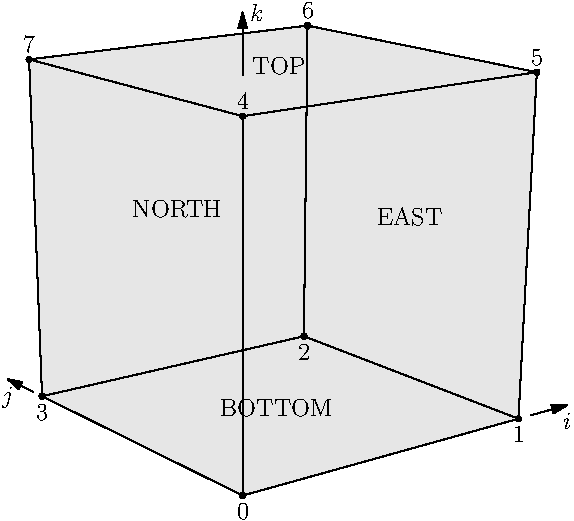
\includegraphics[width=0.5\textwidth]{figs/block3d-defn.pdf}
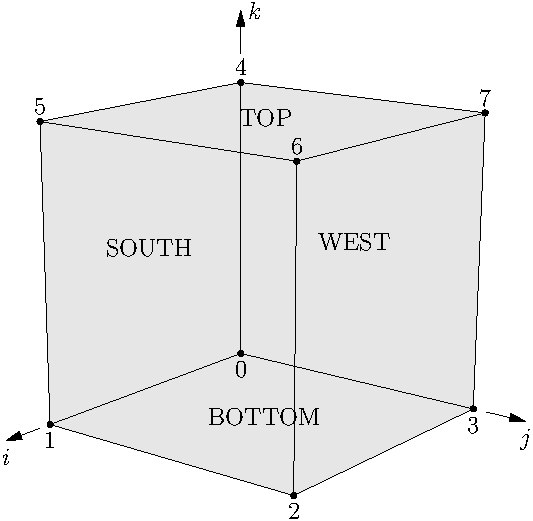
\includegraphics[width=0.5\textwidth]{figs/block3d-defn-2.pdf}
}
\caption{Two views of the hexahedral block containing the structured mesh.
    These figures are ambiguous but each is supposed to show a hollow box
    with the \textit{far} surfaces in each view being labelled.  
    The \textit{near} surfaces are transparent and unlabelled.
    To get your hands on an unambiguous representation, build the debugging cube
    drawn in Appendix\,\ref{cube-development}}.
\label{block-defn-fig}
\end{figure}

\medskip
To define a block in your input script, create a \texttt{Block3D} object as:
\texttt{
\begin{tabbing}
my\_3d\_block = Block3D(\=parametric\_volume=None, grid=None, \\
                        \>import\_grid\_file\_name=None, \\
                        \>nni=None, nnj=None, nnk=None, \\
                        \>cf\_list=[None,]*12, bc\_list=[SlipWallBC(),]*6, \\
                        \>fill\_condition=None, \\
                        \>hcell\_list=None, xforce\_list=[0,]*6, \\
                        \>label="", active=1, omegaz=0.0)
\end{tabbing}\index{block!Block3D}
}
%
\noindent
where the assignment to the name \texttt{my\_3d\_block} allows easy referencing of
the block at later times, say, for adding boundary conditions.
The names of the actual arguments given above match the actual arguments in
the \texttt{e3prep.py} program and these represent\footnote{Again, the
  definitive source is, of course, the \texttt{Block3D} class definition in 
  \texttt{e3\_block.py}. }:
\begin{itemize}
\item \texttt{parametric\_volume}: a region of 3D space bounded by 6 surfaces.
    This is the usual way of specifying the flow domain, which will be discretized 
    using \texttt{nni, nnj, nnk and cf\_list}.
    See the following section for a guide to constructing \texttt{parametric\_volume} objects.
\item \texttt{grid}: a \texttt{StructuredGrid} object may be supplied (defaults to None). 
\item \texttt{import\_grid\_file\_name}\index{import\_grid\_file\_name} defaults to None.
  If a name is supplied, this file is read to obtain the grid directly.
  The assumed file format in the legacy (ASCII) VTK format for a structured grid.
  There is also an external tool (\texttt{p2e.py}) that can be used to convert
  Plot3D format files to Eilmer's native format.
\item \texttt{nni} is the number of finite-volume cells in the $i$-index
  direction as shown in Figure\,\ref{block-defn-fig}.
  This is only used when diecretizing a \texttt{parametric\_volume}.
  When importing or supplying a grid, this data (\texttt{nni, nnj and nnk}) is ignored.
  Note that, when placing one block against another, the blocks must conform in
  \begin{itemize}
    \item the number of cells along corresponding edges
    \item the clustering of those cells along the edges
    \item the path defining the corresponding edges.
  \end{itemize}
\item \texttt{nnj} is the number of finite-volume cells in the $j$-index direction.
\item \texttt{nnk} is the number of finite-volume cells in the $k$-index direction.
\item \texttt{cf\_list} is a list of \texttt{Function} objects
  that specify a (possibly) nonuniform distribution of cells along a
  particular edge of the \texttt{parametric\_volume}.
  The order of the edges is shown in Table\,\ref{edge-list-table}.
  See page~\pageref{cflist-item} for a more complete description of the cluster functions.
\begin{table}
  \caption{Directions for the edges of a \texttt{Block3D} object.}
  \label{edge-list-table}
  \begin{center}
    \begin{tabular}{cccl}
      \hline\hline
      edge & from point & to point & comment \\ 
      \hline
      0  & $p_0$      & $p_1$    & $i$-direction, bottom surface \\
      1  & $p_1$      & $p_2$    & $j$-direction, bottom surface \\
      2  & $p_3$      & $p_2$    & $i$-direction, bottom surface \\
      3  & $p_0$      & $p_3$    & $j$-direction, bottom surface \\
      4  & $p_4$      & $p_5$    & $i$-direction, top surface \\
      5  & $p_5$      & $p_6$    & $j$-direction, top surface \\
      6  & $p_7$      & $p_6$    & $i$-direction, top surface \\
      7  & $p_4$      & $p_7$    & $j$-direction, top surface \\
      8  & $p_0$      & $p_4$    & $k$-direction \\
      9  & $p_1$      & $p_5$    & $k$-direction \\
      10 & $p_2$      & $p_6$    & $k$-direction \\
      11 & $p_3$      & $p_7$    & $k$-direction \\
      \hline \hline
    \end{tabular}
  \end{center}
\end{table}
\item \texttt{bc\_list} is an optional list of BoundaryCondition objects for the 
  six bounding surfaces (\texttt{NORTH, EAST, SOUTH, WEST, TOP, BOTTOM}).
  Available boundary conditions are the same as for Block2D objects
\item \texttt{fill\_condition} is the \texttt{FlowCondition} object with which to
  define the initial flow state within the volume.
  See Section\,\ref{thermo-flow-sec} for defining a suitable flow condition.
  This may also be a callable function that supplies the flow properties as
  a function of position.
\item \texttt{hcell\_list} is a list of ($i,j,k$)-tuples specifying which
  cells should be monitored at simulation time.
  Data from the specified cells will be written to a ``history'' file for the
  block and may be used at the postprocessing stage to provide flow data as if
  there was a sensor located in the cell.
\item \texttt{xforce\_list} is an optional list of zeros/ones that indicate if we
  want the force to be calculated for each of the six surfaces and written to the 
  \texttt{e3shared.log} log file.
  The order of the boundaries is the same as for \texttt{bc\_list}.
\item \texttt{label} is an optional text label for the block.  This label
  will be embedded in the block definition and some of the postprocessing
  programs may use it.
\item \texttt{omegaz} is the rotational speed of the volume about the z-axis.
  This parameter is non-zero only for rotating components of the turbomachine grids.
\end{itemize} 

\medskip
To manually connect particular Block3D objects, you can use the function
\texttt{
\begin{tabbing}
connect\_blocks\_3D(\= A, B, vtx\_pairs, with\_udf=0, filename=None,\\
                    \> is\_wall=0, use\_udf\_flux=0)
\end{tabbing}\index{block!connect\_blocks\_3D}
}
\noindent
where \texttt{A} and \texttt{B} are references to the individual \texttt{Block3D} objects
and \texttt{vtx\_pairs} is a list of 4 pairs (tuples) of vertex indices.
For example, the list \texttt{[(3,2),(7,6),(6,7),(2,3)]} specifies a \texttt{NORTH}-to-\texttt{NORTH} connection
with orientation \texttt{0}.
The definitions of all allowable connections is listed near the top of the file \texttt{e3\_block.py}.
You will see that there are \textit{many} more combinations in 3D compared with 2D.

\medskip
As for the 2D grids, there are two composite-block generation functions.
The first takes a volume, grids it and then subdivides the newly generated grid:
\texttt{
\begin{tabbing}
my\_3d\_block = SuperBlock3D(\=parametric\_volume=None, cf\_list=[None,]*12, \\
                        \>fill\_condition=None, \\
                        \>nni=2, nnj=2, nnk=2, \\
                        \>nbi=1, nbj=1, nbk=1, \\
                        \>bc\_list=[SlipWallBC(),]*6, label="sblk", \\
                        \>hcell\_list=None, omegaz=0.0)
\end{tabbing}\index{block!SuperBlock3D}
}
\noindent
where \texttt{nbi}, \texttt{nbi} and \texttt{nbk} are the number of basic blocks in each of the
index directions.
The values for \texttt{nni}, \texttt{nnj} and \texttt{nnk} specify the number of cells for the grid
generated over the whole volume.
The second composite block takes a volume, subdivides that volume and then generates a separate
grid within each subvolume:
\texttt{
\begin{tabbing}
my\_3d\_block = MultiBlock3D(\=parametric\_volume=None, \\
                        \>fill\_condition=None, \\
                        \>nni=None, nnj=None, nnk=None, \\
                        \>nbi=1, nbj=1, nbk=1, \\
                        \>clusteri=None, clusterj=None, clusterk=None, \\
                        \>bc\_list=[SlipWallBC(),]*6, label="blk", \\
                        \>hcell\_list=None, omegaz=0.0)
\end{tabbing}\index{block!MultiBlock3D}
}
\noindent
Here, \texttt{nni}, \texttt{nnj} and \texttt{nnk} may be integer values or lists of integer values.
If they are simple integers, they represent the number of cells over the whole volume.
If they are lists of integers, they specify the number of cells each of the subblocks.
The \texttt{clusteri}, \texttt{clusterj} and \texttt{clusterk} may be lists of cluster functions
that get applied to the subblocks in the respective index directions.

\noindent
Note the the composite-block objects contain a member \texttt{blks} that refers to the list of basic
blocks that form the composite block.
Any further setting of boundary conditions, and the like, 
needs to be done to the individual blocks within this list.
See the input script for the finite-cylinder case (on page\,\pageref{finite-cyl-script}) for an example of this.

\medskip
When assembling large numbers of blocks for complex geometries, the function
\texttt{
\begin{tabbing}
identify\_block\_connections(\=block\_list=None, exclude\_list=[],\\
                             \>tolerance=1.0e-6)
\end{tabbing}\index{block!identify\_block\_connections}
}
\noindent
also works for 3D blocks.
As for 2D blocks, it performs a brute-force search for all adjacent blocks and sets \texttt{AdjacentBC}
boundary conditions for pairs of faces that have coinciding corners (to within a given tolerance).
The rotational orientation of the joined faces is also determined automatically.
If you don't want the search to be over all blocks generated so far, supply a list to
the \texttt{block\_list} argument.  
Alternatively, supply a list for blocks that should be excluded.

\medskip
Be aware that the \texttt{identify\_block\_connections()} function is unaware of the form of the actual paths
or surfaces connecting the corner points. 
It may be that the corners coincide but the paths and surfaces do not conform.
If you want more control over the process of joining blocks, you can manually
connect blocks using the \texttt{connect\_blocks\_3D()} function which makes the logical
connection without looking at the geometric locations of the corners.
This situation might arise, for example, when you want to apply periodic boundary conditions
\index{boundary conditions!periodic} in the cross-stream direction of a flow domain.
Then, the boundaries that you want to connect have corners and faces that really don't coincide.

%-------------------------------------------------------------------
\bigskip
\section{Setting conditions for individual boundaries}
\label{setting-boundary-conditions-sec}\index{boundary conditions!setting individually}
%
If you have not already set all appropriate boundary conditions through the \texttt{bc\_list}
argument of the block constructor, you may apply boundary conditions to specific faces 
of a \texttt{Block2D} or \texttt{Block3D} object by calling its method
\texttt{
\begin{tabbing}
set\_BC(\=face\_name, type\_of\_BC, inflow\_condition=None, sponge\_flag=None,\\
      \>Twall=None, Pout=None, filename=None, is\_wall=0, use\_udf\_flux=0,\\
      \>label='')
\end{tabbing}\index{boundary conditions!set\_BC}
}
\noindent
and specifying the face and type of boundary condition.
When this function is called, it creates a suitable boundary condition object 
(as discussed in the previous section) and binds it to the appropriate block boundary.
There is no difference in the end result compared with the approach of
specifying the boundary conditions when the block is created. 
\begin{itemize}
  \item \texttt{face\_name}: one of \texttt{NORTH}, \texttt{EAST},
    \texttt{SOUTH}, \texttt{WEST}, \texttt{TOP}, \texttt{BOTTOM}
  \item \texttt{type\_of\_BC}: one of 
    \begin{itemize}
      \item \texttt{ADJACENT}: there is another block abutting this face.
        This boundary condition is usually set by the block-conection functions.
      \item \texttt{SUP\_IN}: supersonic inflow using the
        \texttt{inflow\_condition} properties.
      \item \texttt{EXTRAPOLATE\_OUT}: (assumed) supersonic-outflow where the
        ghost-cell flow properties are simply copies of the adjacent interior 
        cell properties.
      \item \texttt{SLIP\_WALL}: an inviscid solid wall where the normal
        velocity in the ghost cells is a reflection of the velocity in the
        interoir cell.
      \item \texttt{ADIABATIC}: a no-slip wall where the wall temperature is
        the same as the cell-centre temperature.
      \item \texttt{FIXED\_T}: a no-slip wall where the wall temperature is
        specified by \texttt{Twall} in degrees K.
      \item \texttt{SUBSONIC\_IN}: subsonic inflow where the stagnation
        pressure and temperature is specified and the velocity is taken from
        the interior cell.
      \item \texttt{TRANSIENT\_UNI}: a transient flow condition applied
        uniformly across the face of the block.
      \item \texttt{STATIC\_PROF}: a time-invariant flow condition that has
        spatial variation across the face of the block.
      \item \texttt{FIXED\_P\_OUT}: something like the \texttt{EXTRAPOLATE\_OUT}
        condition with the pressure in the ghost cells set to \texttt{Pout}.
      \item \texttt{RRM}: rescaled and recycled data for Andrew Denman's LES simulations.
      \item \texttt{USER\_DEFINED}: the user-supplied Lua functions are used to
        determine ghost-cell flow properties and or interface fluxes.
        These functions are provided in the file given by \texttt{filename}.
        The flag \texttt{is\_wall} indicates whether the boundary is to be considered
        a wall for the application of turbulence-model fudges and the like (default 0).
        The flag \texttt{use\_udf\_flux} indicates whether the user is supplying
        the fluxes at the boundary interfaces (default 0).  
        If not, the internal flux calculator is used together with the supplied ghost-cell data.
      \item \texttt{ADJACENT\_PLUS\_UDF}:
    \end{itemize}
  \item \texttt{inflow\_condition}: the flow condition used for
    \texttt{SUP\_IN}, default value None.
  \item \texttt{sponge\_flag}: Andrew Denman's flag, default value None.
  \item \texttt{Twall}: static temperature of the wall in degrees K, default value None.
  \item \texttt{Pout}: static pressure in Pa applied to the ghost cells, default value None.
  \item \texttt{label}: symbolic label for the boundary, default value is an empty string.
\end{itemize}
You need only specify the properties that are relevant to the specific
boundary condition.

%------------------------------------------------------------------
\bigskip
\section{Special zones and history points}
\label{sec:special-zones}
% 
Zones of heating or cooling may be defined within the flow domain as rectangular (2D) 
or regular hexahedral (3D) patches which are specified by two diagonally-opposite
corners (\texttt{point0} and \texttt{point1}).
For example, we could specify\\
\texttt{HeatZone(qdot, point0, point1, label="")}\index{HeatZone}\\
where \texttt{qdot} is the heat addition per unit volume in W/m$^3$.
The corners of each hexahedral zone are given by the \texttt{Vector} values 
\texttt{point0} and \texttt{point1}.
If the centre of a cell lies within the heat zone, \texttt{qdot} is added to
the source term in the energy equation every time step during the simulation. When using
a HeatZone it is necessary to give at least \texttt{heat\_time\_stop} a positive non-zero
value and \texttt{heat\_time\_start} and \texttt{heat\_factor\_increment} can also be modified
as appropriate.
A HeatZone might be used to model the deposition of energy into a small volume from 
a high-power laser, for example.

\medskip
Similarly, zones of reaction are defined with\\
\texttt{ReactionZone(point0, point1, label="")}\index{ReactionZone}\\
where the finite-rate reactions will be allowed to proceed.
Outside of these zones, the finite-rate chemical update will be suppressed 
and the species concentrations will be effectively frozen.
If no such zones are specified, reactions are permitted for the entire flow field.

\medskip
Also, when running turbulent flow simulations, the turbulence model can also be
restricted to being applied to specific zones using\\
\texttt{TurbulenceZone(point0, point1, label="")}\index{TurbulenceZone}\\
The turbulence model (say, the $k-\omega$ model) is active throughout the flow
but its effect on the flow field is masked outside of the \texttt{TurbulenceZone}s.
This is achieved by the code setting the turbulence viscosity and conductivity to zero
for finite-volume cells that fall outside of all regions defined as a \texttt{TurbulenceZone}.
If there a no such defined regions, all of the flowfield may have nonzero turbulence viscosity.

\medskip
As well as being identified by their cell indices when defining a block,
history points can be located by their Cartesian coordinates using:\\
\texttt{HistoryLocation(x, y, z=0.0, i\_offset=0, j\_offset=0, k\_offset=0, label="")}\index{HistoryLocation} \\
where the offset indices allow you to select a cell a known number of cells 
away from another.

%------------------------------------------------------------------
\bigskip
\section{Simulation control parameters}
\label{sec:sim-control-parameters}
\index{configuration parameters}\index{control parameters}
%
A number of other parameters can be set in order to control the behaviour of
the simulation.
These parameters are mainly collected into the \texttt{gdata}
object\footnote{The \texttt{gdata} object is an instance of the \texttt{GlobalData}
  class defined in \texttt{e3prep.py}. Most of the attributes are discussed here,
  however, see the source code for that class for a full list of attributes.} 
which is accessible to the user's input script.
Grouped by theme, the possible attributes include\footnote{Attributes that are stored in the control file\index{control file}
are denoted by a \ddag ~symbol.  The rest go into the config file.\index{config file}}:
\paragraph{Geometry}
\begin{itemize}
\item \texttt{dimensions}: number of geometric dimensions (2 or 3).  
  If unspecified, the default is 2.
\item \texttt{axisymmetric\_flag}: 1=2D-axisymmetric geometry with $x$-axis being the axis of symmetry,
  0=2D-planar geometry, default value 0.
\end{itemize}

\paragraph{Time stepping}
\begin{itemize}
\item \texttt{sequence\_blocks}: 0=normal time iteration on all blocks, 1=integrate one block
  at a time, default value 0.
\item \texttt{dt}\ddag: the initial time step (in seconds) that will be used for the
  first few steps of the simulation process.
  Be careful to set a value small enough for the time-stepping to be stable.
  Since the time stepping is synchronous across all parts of the flow domain,
  this time step size should be smaller than half of the smallest time for a signal
  (pressure wave) to cross any cell in the flow domain. 
\item \texttt{dt\_chem}: suggested time-step for finite-rate chemistry update;
  default value of -1.0 indicates that we want the code to work it out.
\item \texttt{dt\_therm}: default value -1.0.
\item \texttt{t\_order}\ddag: 1=Euler time stepping, 2=predictor-corrector
  time-stepping, default value 1.
  If you want time-accurate solutions, use predictor-corrector stepping,
  otherwise, Euler stepping is half the computational expense 
  (but you may get less accuracy and the code will not be as robust).
\item \texttt{fixed\_time\_step}\ddag: 1=do not change time step from that specified, 
  0=allow time step size to be determined from cell conditions and cfl number, default value 0.
\item \texttt{cfl}\ddag: ratio of the smallest signal time to the actual time step,
  default value 0.5.
\item \texttt{stringent\_cfl}\ddag: 1=use the smallest cross-cell distance in the
  CFL check, 0=use different cell widths in each index direction, default is 0.
\item \texttt{dt\_reduction\_factor}\ddag: if the CFL condition is violated, scale the time-step size
  down by this factor, default value 0.2.
\item \texttt{cfl\_count}: number of time steps between checks of the CFL
  condition, default value 10.
  This check is expensive so we don't want to do it too frequently but, then,
  we have to be careful that the time step does not become unstable.
\item \texttt{max\_time}\ddag: the simulation will be terminated on reaching this
  value of time, default value $1.0 \times 10^{-3}$.
\item \texttt{t0}: starting time for simulation, may be useful to change when restarting from another job,
  default value 0.0.
\item \texttt{max\_step}\ddag: the simulation will be terminated on reaching this
  number of time steps, default value 10.
\item \texttt{dt\_plot}\ddag: the whole flow solution will be written to disk when
  this amount of simulation time has elapsed, default value $1.0 \times 10^{-3}$s.
\item \texttt{dt\_history}\ddag: the history-point data will be written to disk
  when this amount of time has elapsed, default value $1.0 \times 10^{-3}$s.
\end{itemize}

\paragraph{Spatial reconstruction/interpolation}
\begin{itemize}
\item \texttt{x\_order}\ddag: 1=no reconstruction of intra-cell flow properties
  before applying the flux calculator, 2=high-order reconstruction applied, 
  default value 2
\item \texttt{apply\_limiter\_flag}: 1=apply reconstruction limiter, default value 1.
\item \texttt{interpolation\_type}: string to choose the set of interpolation variables
  to use in the interpolation, options are "rhoe", "rhop", "rhoT", "pT", default value "rhoe".
\end{itemize}

\paragraph{Flux calculator}
\begin{itemize}
\item \texttt{flux\_calc}: selects the flavour of the flux calculator, 
  default value \texttt{ADAPTIVE}.
  The ADAPTIVE scheme is a good all-round scheme that uses AUSMDV away from
  shocks and EFM near shocks.
\item \texttt{compression\_tolerance}: value of relative velocity change (normalised by local sound-speed)
   across a cell-interface that triggers the shock-point detector.  A negative value indicates a compression.
   When the ADAPTIVE flux calculator is used and the shock detector is triggered, the EFM flux calculation
   will be used in place of the default AUSMDV calculation.
   A value of -0.05 seems OK for the sod and cone20 inviscid flow simulations, however,
   a higher value is needed for cases with viscous boundary layers, 
   where it is important to not have too much dissipation in the boundary layer region.
   The default value is -0.30.
\item \texttt{shear\_tolerance}: value of the relative tangential-velocity change 
   (normalised by local sound speed) across a cell-interface that suppresses the use of EFM even if the
   shock detector indicates that EFM should be used for the ADAPTIVE flux calculator.
   The default value is experimentally set at 0.20 to get smooth shocks
   in the stagnation region of bluff bodies.
   A smaller value (say, 0.05) may be needed to get strongly expanding flows to behave 
   when regions of shear are also present.
\end{itemize}

\paragraph{Viscous effects}
\begin{itemize}
\item \texttt{viscous\_flag}: 1=viscous terms are active, 0=inviscid
  simulation, default value 0.
\item \texttt{viscous\_delay}: the time (in seconds) to wait before applying
  the viscous terms.
  This might come in handy when trying to start blunt-body simulations.
\item \texttt{viscous\_factor\_increment}: per-time-step increment of the viscous effects, once
  t\,$>$\,viscous\_delay, default value 0.01.
\item \texttt{diffusion\_flag}: 1=compute multicomponent diffusion of species, default value 0.
\item \texttt{diffusion\_model}: string, default value "None".
\item \texttt{turbulence\_flag}: 1=activate turbulence model, 0=laminar viscosity only,
  default value 0.
\item \texttt{turbulence\_model}: string specifying which model to use, "k\_omega", "baldwin\_lomax",
  default "k\_omega".
\item \texttt{turbulence\_prandtl\_number}: default value 0.89
\item \texttt{turbulence\_schmidt\_number}: default value 0.75
\item \texttt{max\_mu\_t\_factor}: turbulent viscosity is limited to laminar viscosity multiplied
  by this factor, default value 300.0. 
\item \texttt{transient\_mu\_t\_factor}: default value 1.0.
\end{itemize}

\paragraph{Chemistry}
\begin{itemize}
\item \texttt{reacting\_flag}: flag to indicate that the finite-rate chemical
  reactions are active.
  It has a default value of 0, however, it gets set to 1 if the call 
  to \texttt{set\_reaction\_scheme()} is made.
  This is the usual way of setting it.
\item \texttt{reaction\_update}: File name for reaction scheme configuration.
  (More conveniently set by calling \texttt{set\_reaction\_scheme()}.)
\item \texttt{reaction\_time\_start}: time after which finite-rate reactions are allowed to start,
  default value 0.0.
\end{itemize}

\paragraph{Miscellaneous}
\begin{itemize}
\item \texttt{title}: a title string that may appear in a number of places.
  For example, in plots made during the postprocessing stage.
\item \texttt{max\_invalid\_cells}: the maximum number of bad cells that will be tolerated on
  decoding conserved quantities.  It this number is exceeded, the simulation will stop. default value 10.
\item \texttt{udf\_source\_vector\_flag}: 1=apply user-defined source terms as supplied in a Lua file,
  default value 0.
\item \texttt{udf\_file}: name of the Lua file for the user-defined source terms, default value "".
\item \texttt{print\_count}\ddag: number of time steps between printing status
  information to the console, default value 20.
\item \texttt{heat\_time\_start}: default value 0.0, in seconds.
  For a description of HeatZones, see Section\,\ref{sec:special-zones}.
\item \texttt{heat\_time\_stop}: a non-zero value indicates that we wish to add heat
  through the HeatZones, default value 0.0, in seconds.
\item \texttt{heat\_factor\_increment}: the fraction of full heat load that will be
  added with each step after $t$=heat\_time\_start, default value 0.01.
\end{itemize}


%------------------------------------------------------------------
\section{Parameters for a 2D sketch of the flow domain}\index{sketch}
%
The \texttt{sketch} object holds parameters that set the view and scale of the
SVG (scalable vector graphic) rendering of the two-dimensional flow domain.
The method
\texttt{
\begin{tabbing}
sketch.window(\=xmin=0.0, ymin=0.0, xmax=1.0, ymax=1.0,\\
              \>page\_xmin=0.05, page\_ymin=0.05, page\_xmax=0.17, page\_ymax=0.17)
\end{tabbing}
}

\noindent
sets the mapping from the lower-left to upper-right points in simulation geometry 
to the corresponding points on a page.
Axes may also be drawn with:\\
\texttt{sketch.xaxis(x0, x1, xtic, y\_offset)} \\
\texttt{sketch.yaxis(y0, y1, ytic, x\_offset)} \\
where small negative values may be given for the offset values in order to move
the axes clear of the main sketch elements.

\medskip
Of course, this sketch environment is only available for 2D simulations.
For 3D rendering, there is an option for most geometric elements to be rendered as
Virtual Reality Markup Language (VRML) strings.\index{VRML}  
These VRML strings may be manually written to a file as part of the user's input script.
 
\cleardoublepage
%-------------------------------------------------------------------
% The examples...

\part{Examples for 2D flow}
%
These examples are graded from simple geometry specification and gas model specification
to more complex.
Initially, simple box regions and single-specied ideal gas models are used, followed by
examples with curved boundaries, equilibrium gas models and, also, 
multi-species thermally-perfect gases with finite-rate chemical kinetics.
Later examples also use more of Python's capabilities with the input script for the 
heat-transfer to a sphere, for example, being written as a template script and a top-level 
coordinating script that runs the simulation a number of times with better grid resolution.

% 2D examples
% cone20-simple.tex

\section{Mach 1.5 flow over a 20-degree cone -- Simple boundaries}
\label{cone20-simple-sec}
%
Let's start with a simple-to-imagine flow of ideal air over a sharp-nose of a supersonic projectile.
Figure\,\ref{cone20-flight-fig} is a reproduction of Fig.\,3 from Maccoll's 1937 paper\,\cite{maccoll_1937a} 
and shows a shadowgraph image of a two-pounder projectile, in flight at Mach 1.576.
We'll restrict our simulation to just the gas flow coming onto and moving up the conical surface 
of the projectile and work in a frame of reference attached to the projectile.
Further, we will assume that all of the interesting features of the three-dimensional flow can be 
characterized a two-dimensional plane.
The red lines mark out the region of our gas flow simulation, 
assuming axial symmetry about the centreline of the projectile.

\begin{figure}[htbp]
\begin{center}
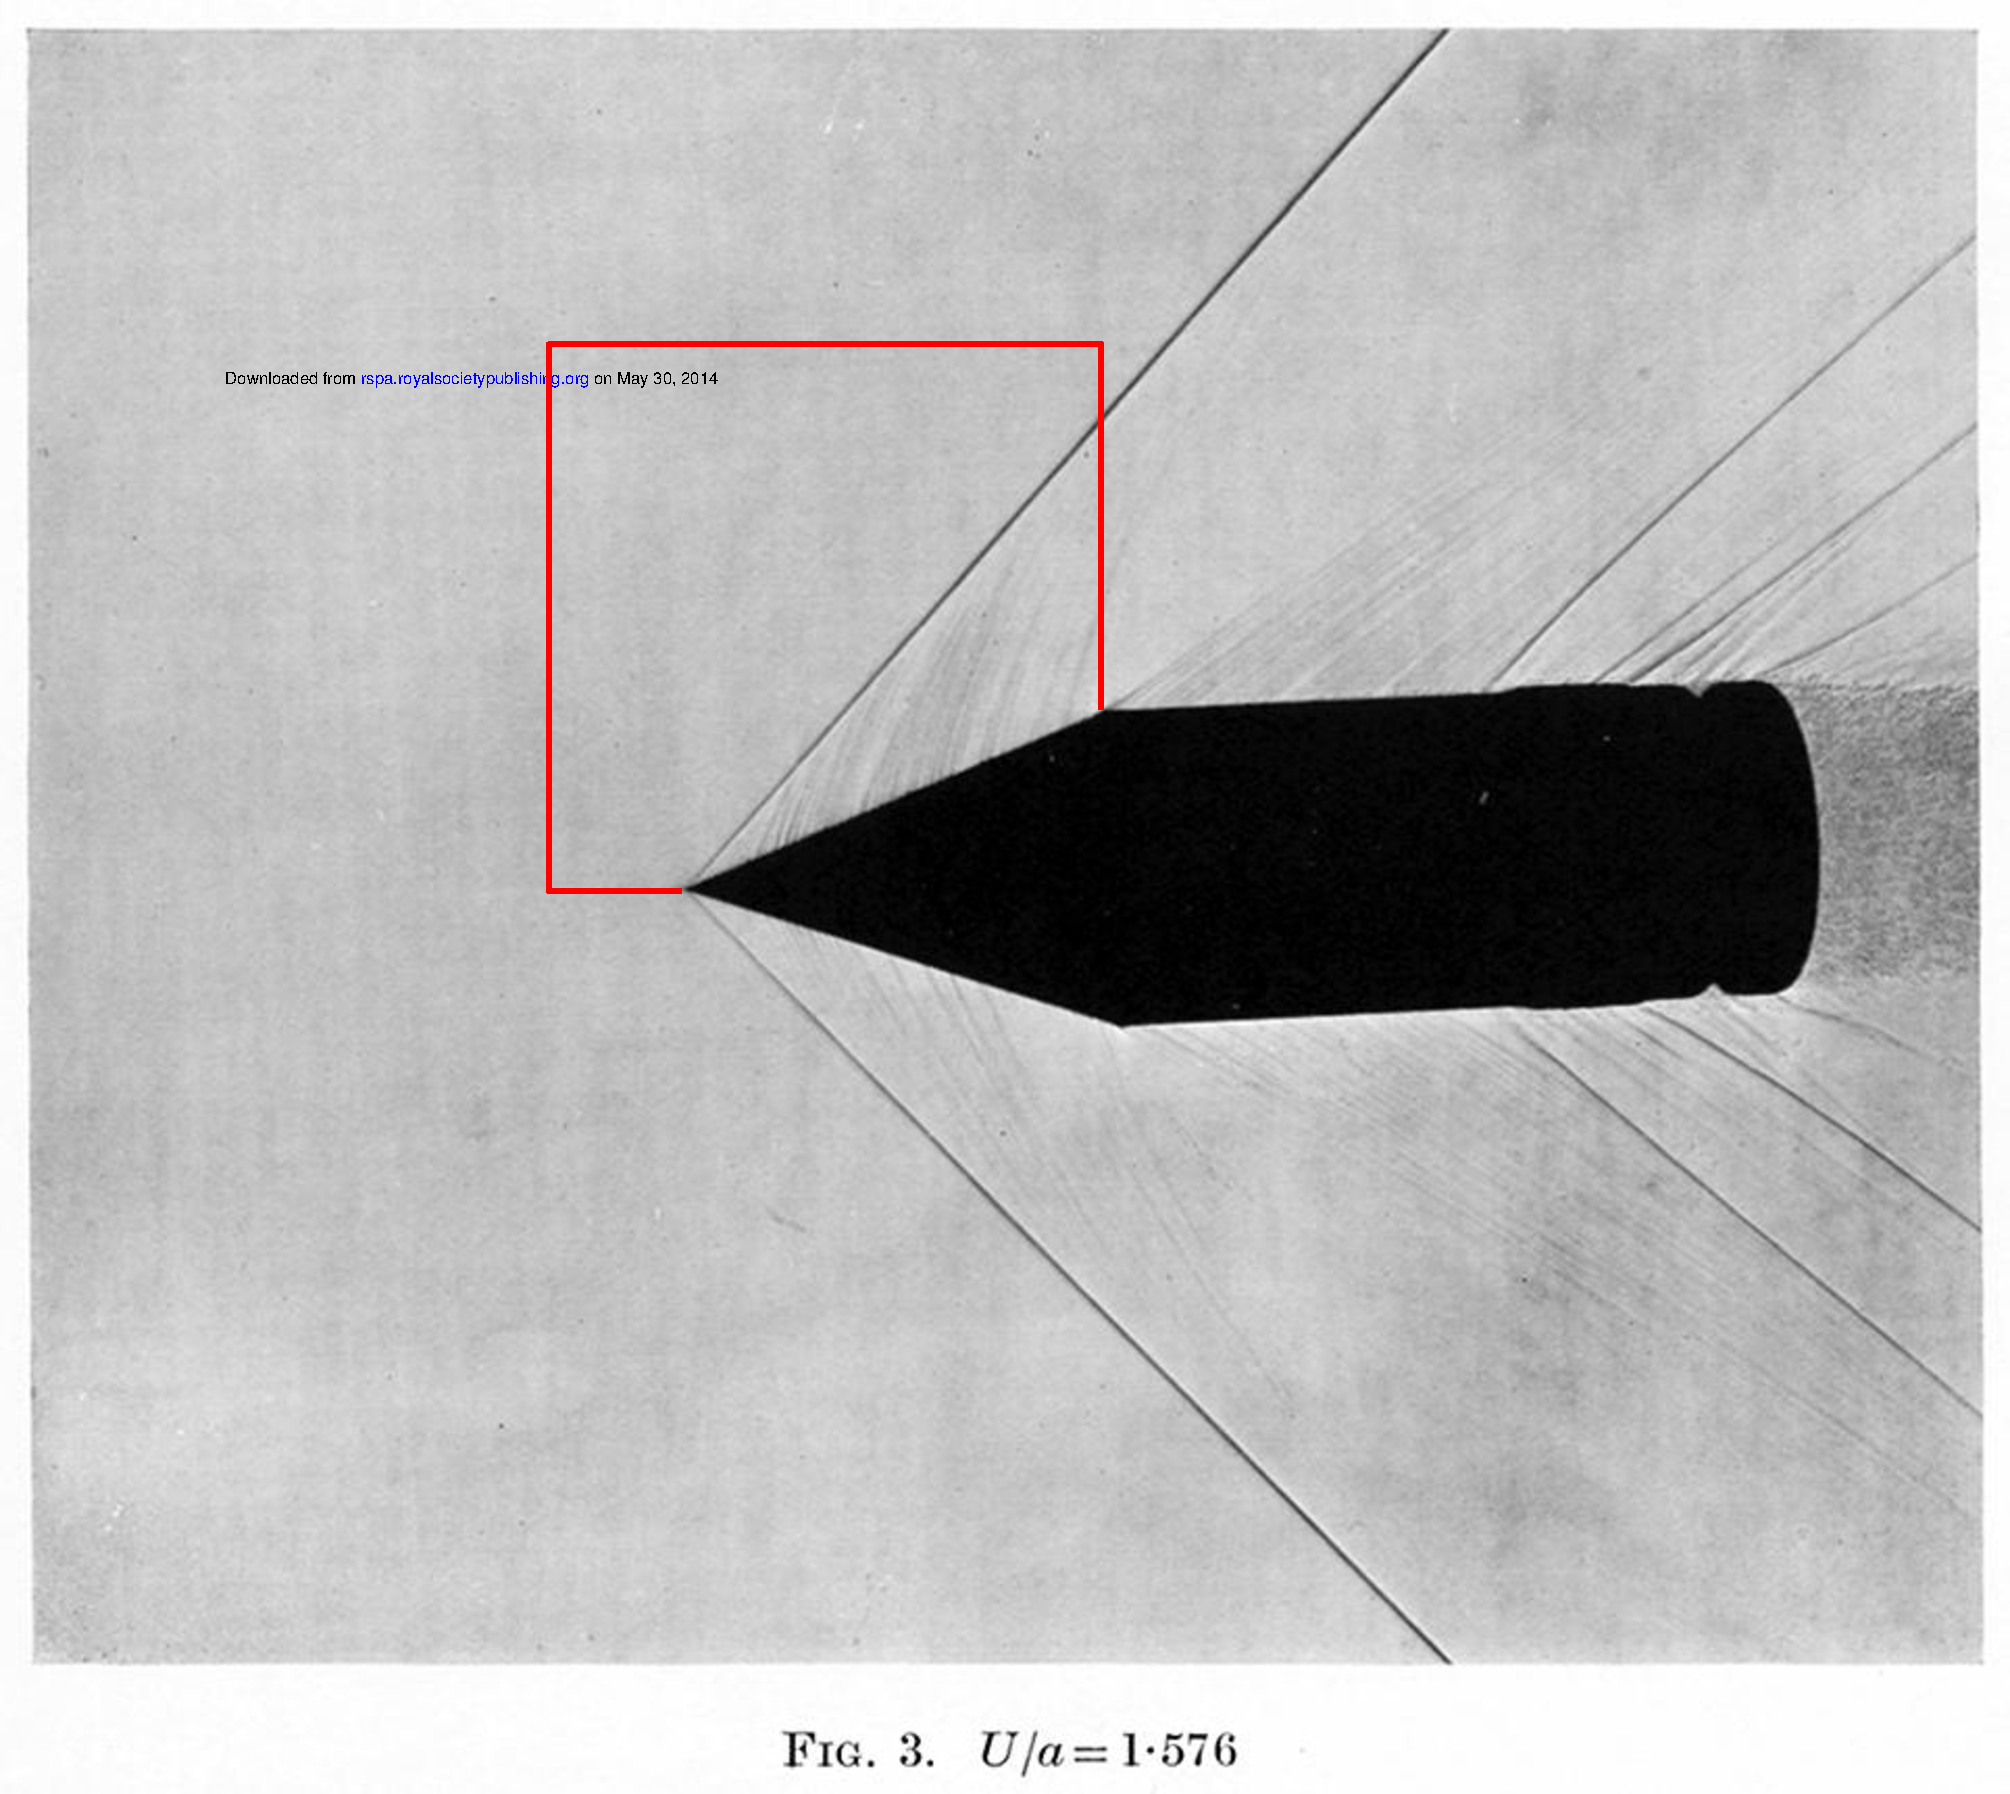
\includegraphics[width=0.9\textwidth, viewport=76 168 949 761, clip=true]{../2D/cone20-simple/maccoll-1937-fig3.pdf}
\end{center}
\caption{A two-pound projectile in flight.  A conical shock is attached to the sharp nose of the projectile. 
	 This photograph was published by Maccoll in 1937.
	 The red lines have been added to demark the region of gas flow for which we will set up our simulation.}
\label{cone20-flight-fig}
\end{figure}

\subsection{Input script (.py)}\index{boundary conditions!set\_BC!example of use}
%
To build our simulation, we abstract the boxed region from Figure\,\ref{cone20-flight-fig}
and consider the axisymmetric flow of an ideal, inviscid gas over a sharp-nosed cone 
with 20 degree half angle.
With the constraint of axisymmetry implies zero angle of incidence for the original 3D flow.

\medskip
The resulting flow, in the steady-state limit, should have a single shock that is 
straight in this 2D meridional plane (but conical in the original 3D space).
The angle of this shock can be checked against Taylor and Maccoll's gas-dynamic theory and,
since the simulation demands few computational resources (in both memory and run time), 
it is useful for checking that the simulation and
plotting programs have been built and installed correctly.

\begin{figure}[htbp]
\begin{center}
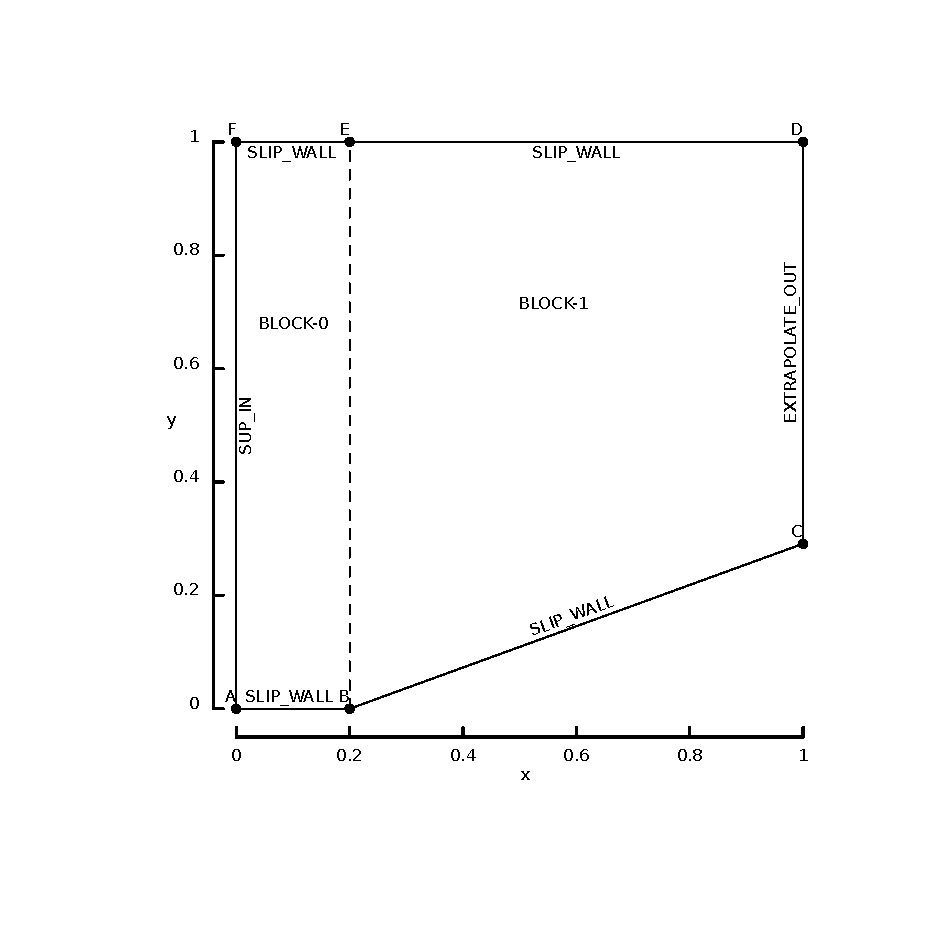
\includegraphics[width=10cm, viewport=76 78 389 398]{../2D/cone20-simple/cone20_svg.pdf}
\end{center}
\caption{Schematic diagram of the geometry for a cone 
         with 20 degree half-angle.
	 This PDF figure was generated from the SVG file with some edits 
	 to move the boundary labels to nicer positions.}
\label{cone20-geometry-fig}
\end{figure}

\noindent\topbar
\lstinputlisting[language={}]{../2D/cone20-simple/cone20.py}
\bottombar

\medskip
Despite Figure\,\ref{cone20-flight-fig} being a good motivator for this simulation,
the free-stream conditions of $p_{\infty} = 95.84$\,kPa, $T_{\infty} = 1103$\,K
and $u_{\infty} = 1000$\,m/s are actually related to the shock-over-ramp test problem
in the original ICASE Report\,\cite{jacobs_91d} and are set to give a Mach number of 1.5.
It is left as an exercise for the reader to run a simulation at Maccoll's value of
Mach number and check that the simulation closely matches the shadowgraph image.


\subsection{Running the simulation}
%
Assuming that you have the program executable files built and
accessible on your system's search \texttt{PATH}, as described in Appendix\,\ref{getting-started-file},
try the following commands:\\
%
\topbar\\
\texttt{\$ cd $\sim$/cfcfd3/examples/eilmer3/2D/cone20-simple/}\\
\texttt{\$ ./cone20\_run.sh}\\
\bottombar\\
%
and, within a minute or so, you should end up with a number of files
with various solution data plotted.
The grid and initial solution are created and the time-evolution of the
flow field is computed for 5\,ms (with 862 time steps being required).
The commands invoke the shell script shown below.
This script, less the commands to generate the plot, could be used as
a template for your own simulation shell scripts.

\noindent \topbar
\lstinputlisting[language={}]{../2D/cone20-simple/cone20_run.sh}
\bottombar

\subsection{Results and Postprocessing}
%
Figure\,\ref{cone20-low-res-fig} shows the flow field 5\,milliseconds after flow start.
This has been long enough for the flow to reach a steady state, with the shock being essentially straight.
The plots have been produced with \verb!Paraview!, picking up the \verb!plot/cone20.pvd! file.
The time stamp in the lower left corner has been added as an \verb!Annotate Time Filter!, 
selected from the main \verb!Filters! menu.
Also, the pressure field has been plotted as a coloured \verb!surface!, 
while the temperature field has been plotted as a \verb!surface with edges!
to clearly show the computational grid.
The distortion of the grid in the right-hand block is a result of the area-orthogonality (AO) grid generator
making the compromises required to achieve a reasonably-orthogonal mesh at the edges of the block.
The default transfinite grid generator would have produced a mesh that appears less distorted
overall but would have individual cells that are more sheared for this particular block.
For the rectangular block on the left, both generators would produce the same mesh.

\begin{figure}[htbp]
\begin{center}
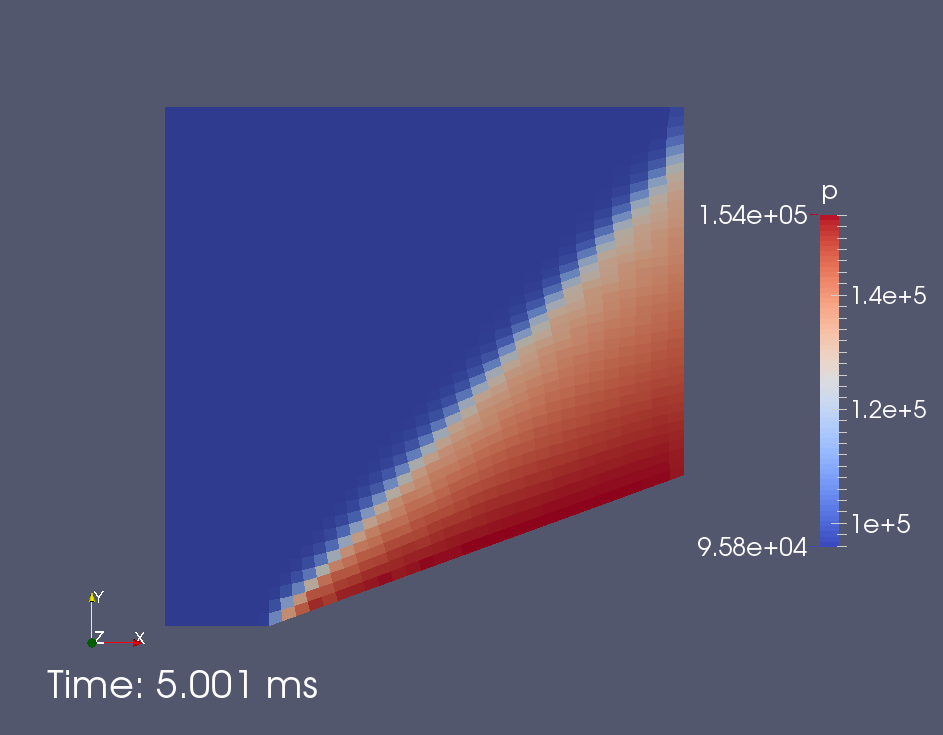
\includegraphics[width=0.45\textwidth]{../2D/cone20-simple/cone20_p.png}
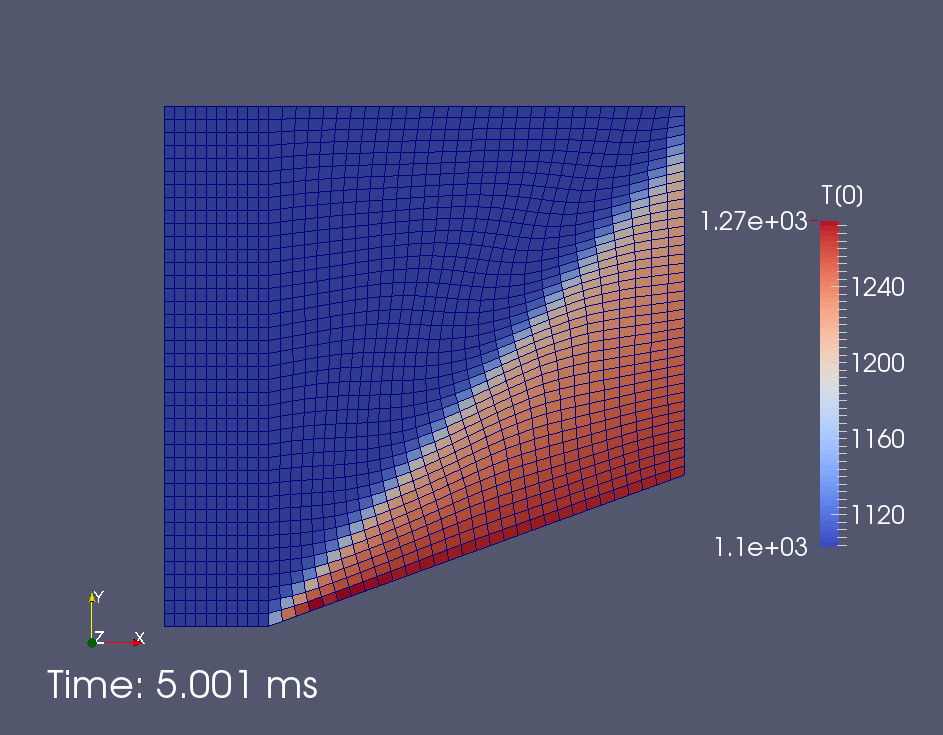
\includegraphics[width=0.45\textwidth]{../2D/cone20-simple/cone20_T0_with-mesh.png}
\end{center}
\caption{Pressure and temperature fields for a low-resolution simulation 
         of flow over a cone with 20 degree half-angle.
         The temperature field plot also included the mesh.}
\label{cone20-low-res-fig}
\end{figure}

% \begin{figure}[htbp]
% \begin{center}
% 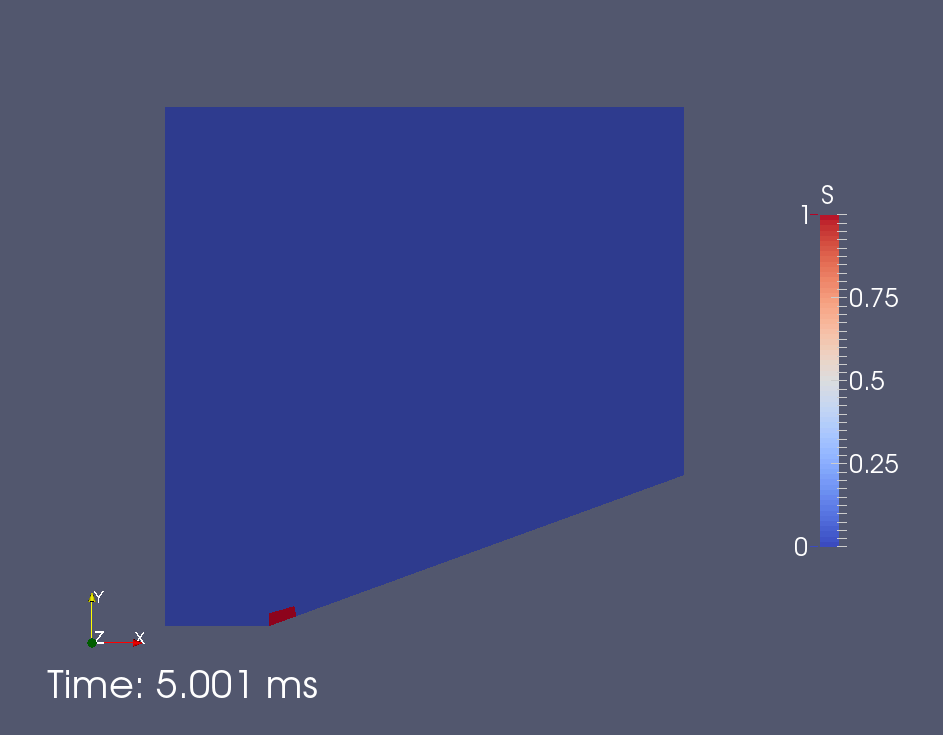
\includegraphics[width=0.8\textwidth]{../2D/cone20-simple/cone20_S.png}
% \end{center}
% \caption{Shock-sensor data for flow over a cone with 20 degree half-angle.
%          For the \texttt{adaptive} flux calculator, 
% 	 this sensor indicates the regions
%	 of the flow where the more dissipative scheme should be used.}
% \label{cone20-shock-sensor-fig}
% \end{figure}

\medskip
The shock displayed in the pressure field shows features that are characteristic 
of a flow solution produced by a ``shock-capturing'' code such as \verb!Eilmer3!.
With the coarse grid, the shock has a stair-case appearance.
This is accentuated by the plotting program which was set to display 
the cell-average value as a uniform colour within each cell.
Also, when following a line that crosses the shock,
a small number of cells to be counted before the full pressure jump has been reached.
In an ideal, inviscid simulation, the shock should be a zero-thickness transition.
This can be approached by increasing the mesh resolution, as seen in Figure\,\ref{cone20-high-res-fig}.
The high-resolution solution is looking clean but the computational cost, in terms of time, 
has gone up from a few seconds to nearly 2 hours.

\begin{figure}[htbp]
\begin{center}
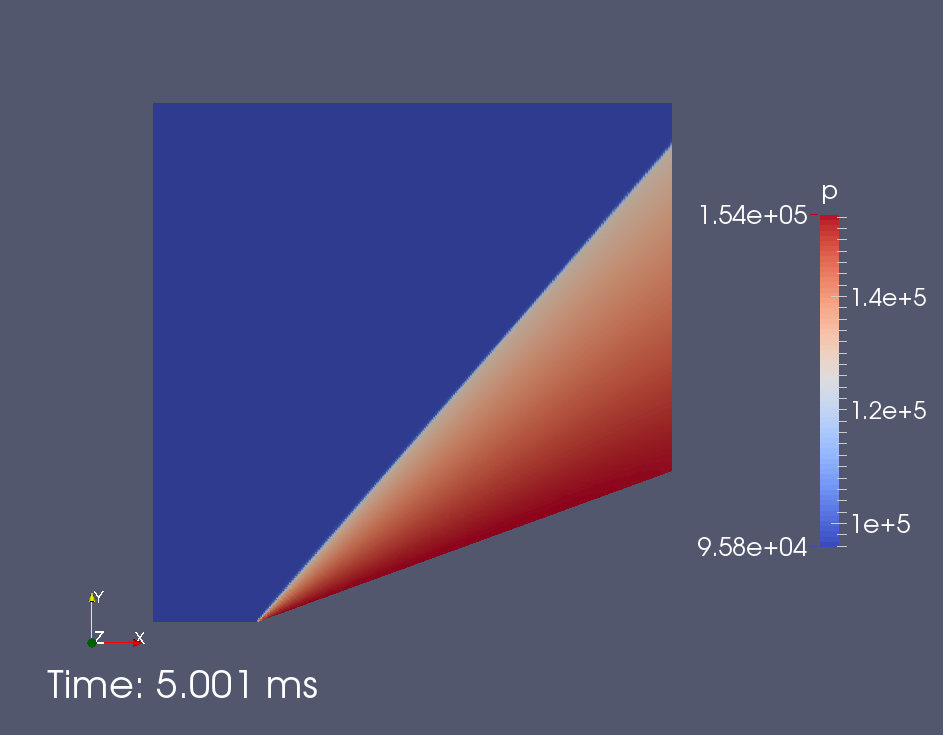
\includegraphics[width=0.45\textwidth]{../2D/cone20-simple/cone20_p_factor-8-grid-res.png}
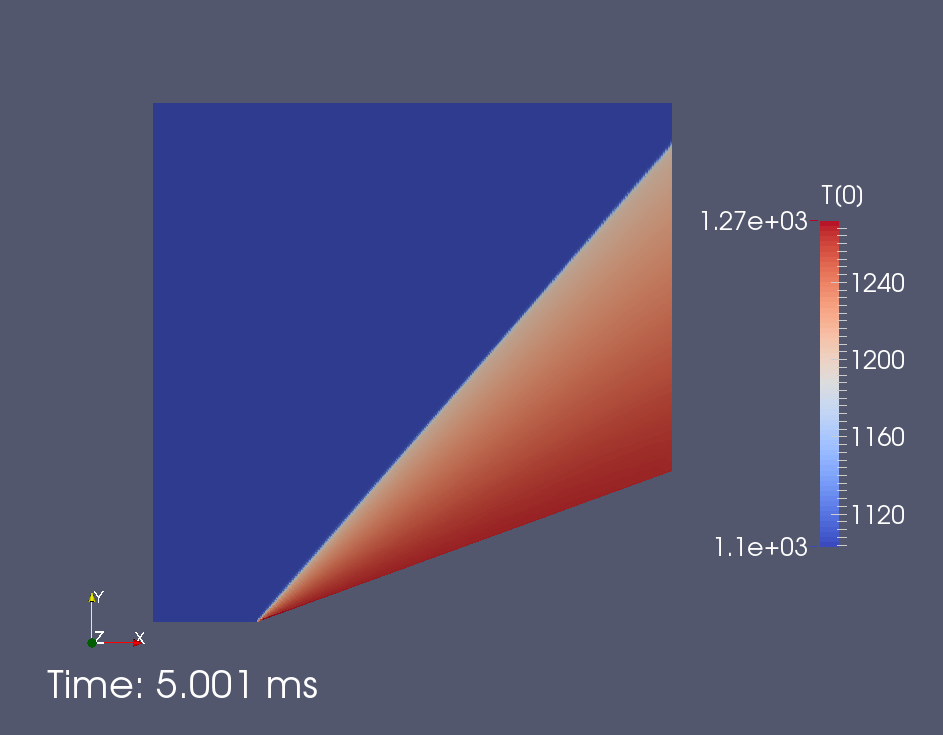
\includegraphics[width=0.45\textwidth]{../2D/cone20-simple/cone20_T0_factor-8-grid-res.png}
\end{center}
\caption{Pressure and temperature fields for a mesh with 8 times more resolution in each direction.}
\label{cone20-high-res-fig}
\end{figure}

\medskip
Since Eilmer3 is a simulation program, it starts with some initial (but possibly variable) 
flow state across the whole simulation domain and then, subject to the applied boundary conditions,
integrates the conservation equations for in a \textit{time-accurate} manner.
In this case of a constant free stream flow coming onto a sharp cone, the flow field evolves toward 
a steady state.
A key flow parameter of interest might be the drag on the cone and we can get \verb!Eilmer3! to
occasionally write out the integrated forces on the cone surface with the \verb!xforce_list = [0,0,1,0]!
argument used when constructing the second block.
This causes \verb!Eilmer3! to write the integrated forces to the log file 
at the same frequency as history files are written.
We then use an Awk program (\verb!cp.awk!) to filter the log file, 
extracting lines that have the x-force data of interest.
New users might like to use an equivalent program written in Python.

\noindent \topbar
\lstinputlisting[language={}]{../2D/cone20-simple/cp.awk}\index{xforce\_list!example of use}
\bottombar
      
\medskip
Before plotting the drag force history, 
it is convenient to normalize it into a history of drag coefficient.
From Chart 5 in Ref.\,\cite{ames_53}, the expected steady-state shock wave
angle is 49$^o$ and, from Chart 6, the pressure coefficient is
$$
\frac{p_{cone-surface} - p_{\infty}}{q_{\infty}} \approx 0.387
$$
and the dynamic pressure for the specified free stream is
$q_{\infty} = \frac{1}{2} \rho_{\infty} u_{\infty}^2 \approx 151.38$\,kPa.
Figure~\ref{cone20-axial-force-fig} shows the pressure coefficient 
estimated as
$$
C_p = \frac{f_x - p_{\infty} A}{q_{\infty} A}
$$
from the simulated axial force, $f_x$, written into the simulation log file
and frontal area of the cone, $A$.
Note the sudden rise as the shock structure driven by the free-stream flow
arrives at the cone surface.
There is a more gradual rise after this initial jump as the conical flow region
fills out and becomes steady.

\begin{figure}[htbp]
\begin{center}
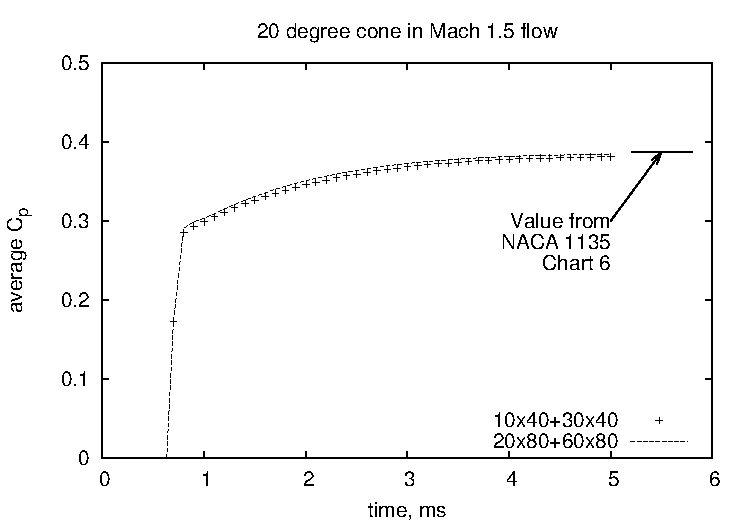
\includegraphics[width=10cm]{../2D/cone20-simple/cone20_cp.pdf}
\end{center}
\caption{Evolution of the axial (drag) force
         for flow over a cone with 20 degree half-angle
	 for two mesh resolutions.}
\label{cone20-axial-force-fig}
\end{figure}

\subsection{Accessing the field data for specialized postprocessing}
%
Beyond the usual slice-and-dice type of postprocessing that is provided by \verb!e3post.py!, 
it may be useful to do specialized calculations on the flow data.
In this flow, the shock is expected to be straight and we can compute
that it should have an angle of $\beta = 48.96^o$, with respect to the free-stream direction,
using one of the gas-dynamic functions\footnote{For documentation on the functions in \texttt{cfpylib},
look at the web site \texttt{http://cfcfd.mechmining.uq.edu.au/} under the heading \texttt{Libraries}.} 
from \verb!cfpylib!
\begin{verbatim}
from cfpylib.gasdyn.ideal_gas_flow import beta_cone
from math import degrees, radians
beta = beta_cone(V1=1000.0, p1=95.84e3, T1=1103.0, theta=radians(20.0))
print "beta=", degrees(beta), "degrees"
\end{verbatim}

The \texttt{estimate\_shock\_angle.py} script uses the Python code libraries 
that the \texttt{e3post.py} is built upon to pick up the data, 
locate the shock position along each strip of cells in the x-direction,
and then fit a straight line to the collected points.
Note that the points from the top right of the flow solution are omitted from the straight-line fit
because the top boundary has interfered with the flow.
The shock points and the fitted line are shown in Fig.\ref{cone20-shock-points-fig} 

\begin{figure}[htbp]
\begin{center}
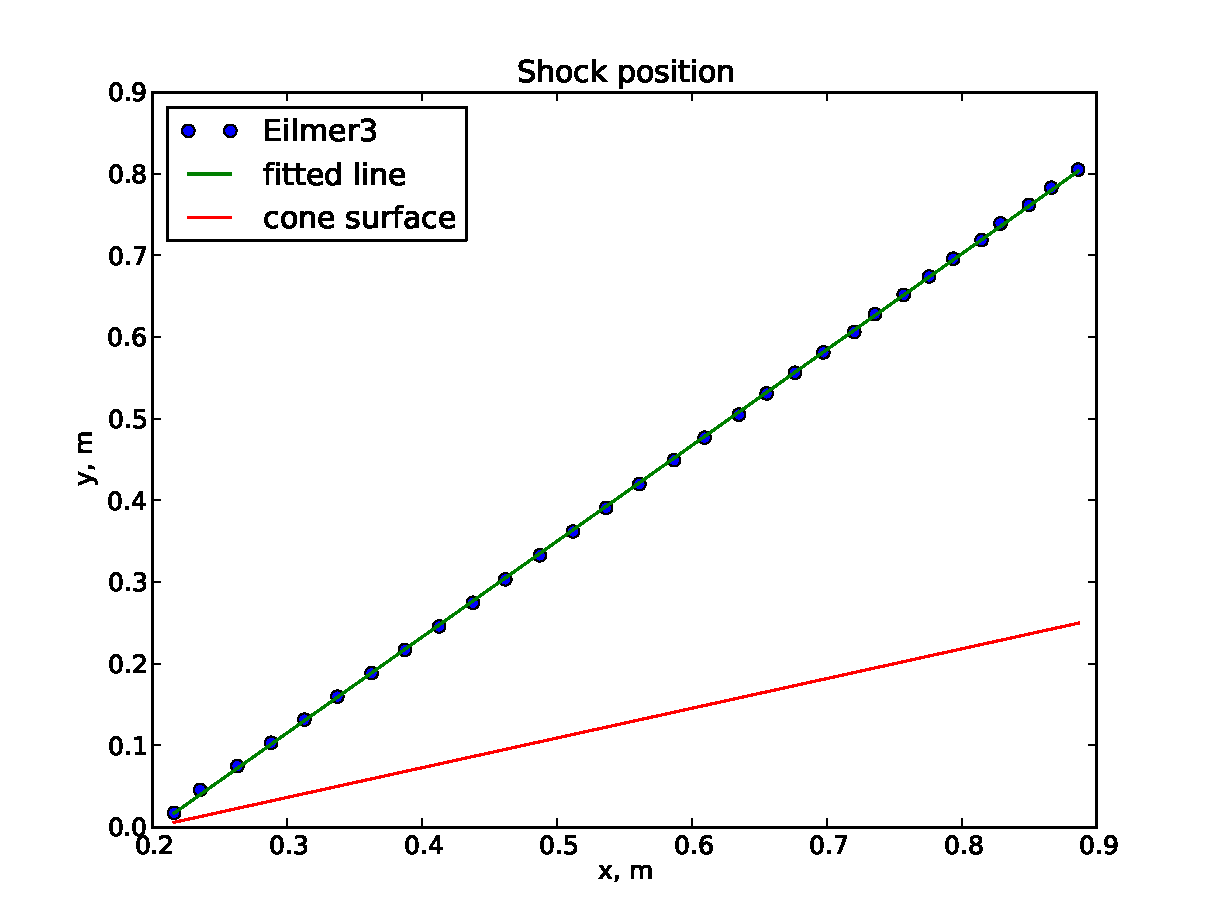
\includegraphics[width=10cm]{../2D/cone20-simple/shock-shape.pdf}
\end{center}
\caption{Shock shape for Mach 1.5 flow over the 20-degree cone.}
\label{cone20-shock-points-fig}
\end{figure}

The script below uses the data reading and storage capability provided by 
the class \texttt{StructuredGridFlow}, which is imported from \texttt{e3\_flow.py}.
Given a file containing the flow data for a block of cells, this class has a \texttt{read} 
method that picks up the data.
The flow and position data is stored in a dictionary, with one multidimensional numpy array 
for each variable.
Access to the pressure in cell \texttt{i,j,k} of block \texttt{ib,jb} is achieved by
putting these indices together as \texttt{blockData[ib][jb].data['p'][i,j,k]}.
The core of the data handling is in the function \texttt{locate\_shock\_front()}
in the middle of the script.

\noindent
\topbar
\lstinputlisting[language={}]{../2D/cone20-simple/estimate_shock_angle.py}
\bottombar

\subsection{Grid convergence}
%
Determining a single value for some parameter is only part of the complete job.
Usually, you must provide some guide as to the reliability of that value and
this is often done with a grid convergence study.
For our estimate of shock wave angle, we could follow the initial simulation run with a 
number of runs on successively finer meshes and check that the estimated values converge 
in the limit of cell size going to zero.

\medskip
Since this example is not very demanding for low-resolution grid, 
it is easy to double the grid resolution a couple of times over and get
data over a good range of cell sizes.
Figure\,\ref{cone20-grid-convergence-fig} shows the raw shock angle estimates
converging nicely to a value of 49$^o$.
In general, this is usually the end point for our analysis.
Since we have a reference value computed via the Taylor-Maccoll theory,
we can also look at the convergence to the \textit{true} value and,
given sufficient computational resource, 
it looks at though we can get as close as we wish.

\begin{figure}
 \centering
 \parbox{0.45\textwidth}{
 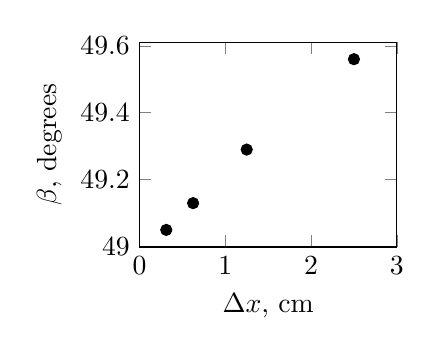
\begin{tikzpicture}
  \begin{axis}[xlabel={$\Delta x$, cm},
               ylabel={$\beta$, degrees},
               xmin=0, xmax=3,
               width=0.4\textwidth]
   \addplot[only marks,mark=*] coordinates{
    (2.5, 49.56)
    (1.25, 49.29)
    (0.625, 49.13)
    (0.3125, 49.05)
   };
  \end{axis}
 \end{tikzpicture}
 }
 \parbox{0.45\textwidth}{
 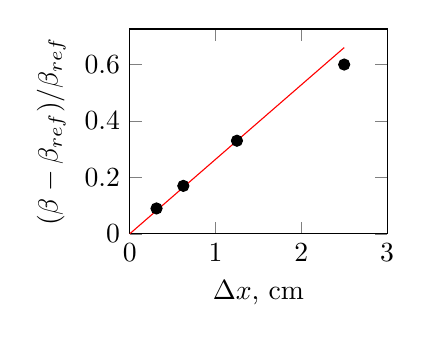
\begin{tikzpicture}
  \begin{axis}[xlabel={$\Delta x$, cm},
               ylabel={$(\beta - \beta_{ref}) / \beta_{ref}$},
               xmin=0, xmax=3, ymin=0,
               width=0.4\textwidth]
   \addplot[only marks,mark=*] coordinates{
    (2.5, 0.6)
    (1.25, 0.33)
    (0.625, 0.17)
    (0.3125, 0.09)
   };
   \addplot[no marks, color=red, smooth, domain=0:2.5]{0.264*x};
  \end{axis}
 \end{tikzpicture}
 }
 \caption{Convergence of the shock angle and its relative error with mesh refinement.
          $\beta_{ref} = 48.96^o$.}
 \label{cone20-grid-convergence-fig}
\end{figure}


\subsection{Notes}
\begin{itemize}
\item Remember that long-format command-line options start with two dashes.
      For example \texttt{--job=cone20}.
      These double dashes are a little hard to distinguish in the shell
      scripts.

\item Run time is approximately 17 seconds for 862 steps on a computer with 
      an AMD Phenom II X4 840, 800\,MHz processor.
      Of course, the shared-memory code does not make use of the other 4 processor cores,
      however, there is an MPI version of the code that can.

\item This cone20.py file really has full access to the Python interpreter
      on your system.  Later examples will show how to use Python to write
      data files from within the input script.  Be careful.

\item Python is a dynamic language.
      It is easy to bind names to new objects within your script.
      Be careful that you do not rebind essential names that will be
      later used by the \texttt{e3prep.py} program.
      Where this might happen in a non-obvious way is in the importing
      of foreign modules (to do something interesting in your script)
      with the command ``from \textit{module-name} import *''.

\item The script \texttt{cone20\_run\_mpi.sh} is available for running the simulation
  with the parallel version of the code on a machine with OpenMPI installed.
  This script is essentially the same as shown for the shared-memory simulation
  with the MPI simulation being started with the commands:\index{e3mpi.exe!example of use}
\begin{verbatim}
mpirun -np 2 e3mpi.exe -f cone20 --run
\end{verbatim}
  The only other modification required is to look for the surface-force data in the
  log file \texttt{e3mpi.0001.log} rather than \texttt{e3shared.log}.

\end{itemize}

\cleardoublepage
% axi-cylinder.tex

\newpage
\section{Viscous Flow Along a Cylinder}
\label{axi-cylinder-sec}
%
This case (\texttt{2D/axi-cylinder/} computes the flow for
a supersonic laminar boundary layer growing along a hollow cylinder.
It was used in the original report\cite{jacobs_91d} to verify the implementation of
the viscous and axisymmetric terms in the code.

\begin{figure}[htbp]
\begin{center}
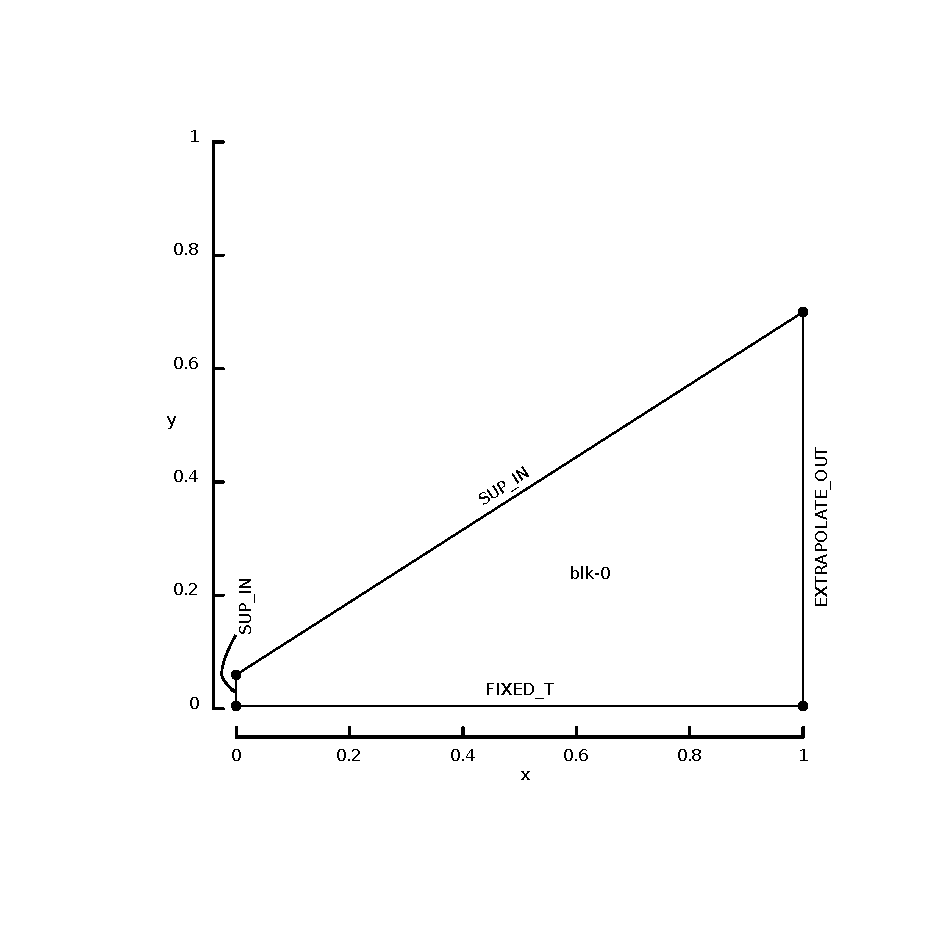
\includegraphics[width=0.7\textwidth,viewport=79 77 400 392,clip=true]{../2D/axi-cylinder/cyl50.pdf}
\end{center}
\caption{Flow domain for viscous flow along a cylinder.}
   \label{cyl50-layout-fig}
\end{figure}

\medskip
The flow geometry consists of a hollow cylinder, 1.0m long with
radius 0.005m, aligned with the $x$-axis.
The flow domain shown in Figure~\ref{cyl50-layout-fig} is defined
by a quadrilateral with corners (1.0,~0.005), (1.0,~0.7),
(0.0,~0.06), (0.0,~0.005).
This region is shaped to capture the weak leading-edge-interaction shock 
while concentrating cells near the cylinder surface for the early part of the boundary layer development.
The grid consists of $50 \times 50$ cells which are clustered toward
the leading edge of the cylinder and 
(even more strongly in the $y$-direction) toward the cylinder surface.

\medskip
The free stream is a uniform supersonic flow of air, modelled
as a perfect gas with conditions
$$
   \rho = 0.00404~ {\rm kg/m^3},~~
   u_x = 597.3~ {\rm m/s}, ~~
   u_y = 0, ~~
   e = C_v T = 1.592 \times 10^5 ~ {\rm J/kg},
$$
%
$$
   T = 222~ {\rm K}, ~~
   p = 257~ {\rm Pa}, ~~
   M = 2.
$$
This free stream condition is applied to the West and North
boundaries, the East boundary is a supersonic outflow boundary and
the South boundary (along the cylinder surface) is a no-slip
boundary with temperature fixed at $T = 222~\rm K$.
The Reynolds number at the end of the plate is $1.65 \times 10^5$.

\medskip
Initially, the flow throughout the block is set at the same conditions
as the free stream and the governing equations are integrated in time.
Figure~\ref{cyl50-flow-field-fig} shows the pressure and temperature fields
after a period of 8\,ms.
The weak leading-edge interaction shock is most clearly seen in the pressure field
and the boundary layer on the cylinder surface is evident in the temperature field.

\begin{figure}[htbp]
\mbox{
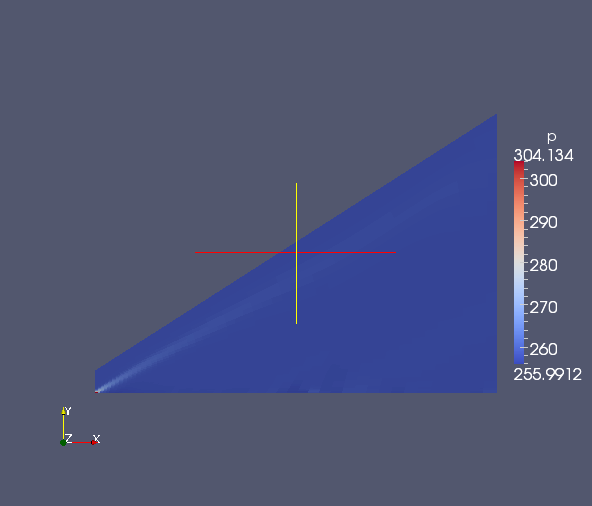
\includegraphics[width=0.5\textwidth]{../2D/axi-cylinder/cyl50-t8ms-p.png}
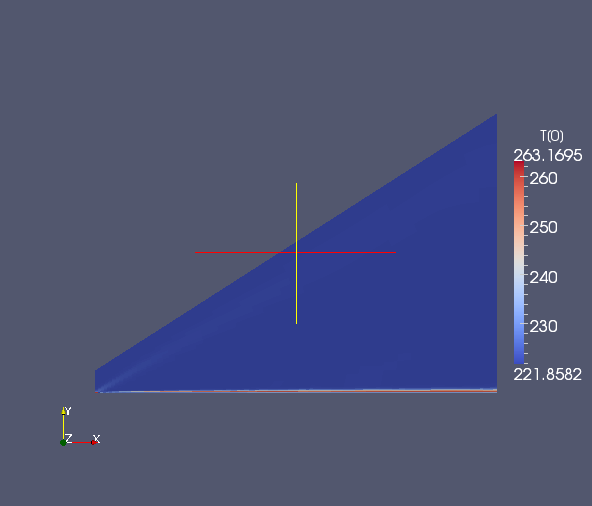
\includegraphics[width=0.5\textwidth]{../2D/axi-cylinder/cyl50-t8ms-T.png}
}
\caption{Pressure and temperature fields for viscous flow along a cylinder.}
   \label{cyl50-flow-field-fig}
\end{figure}

\medskip
Figure \ref{cyl50-profiles-fig} shows the $x$-velocity and temperature profiles
through the boundary layer at $x$=0.916\,m, 
48 cells from the leading edge of the cylinder.
The simulation data from \texttt{Eilmer3} are compared with data produced by David Pruett's
spectral boundary layer code.

\begin{figure}[htbp]
\mbox{
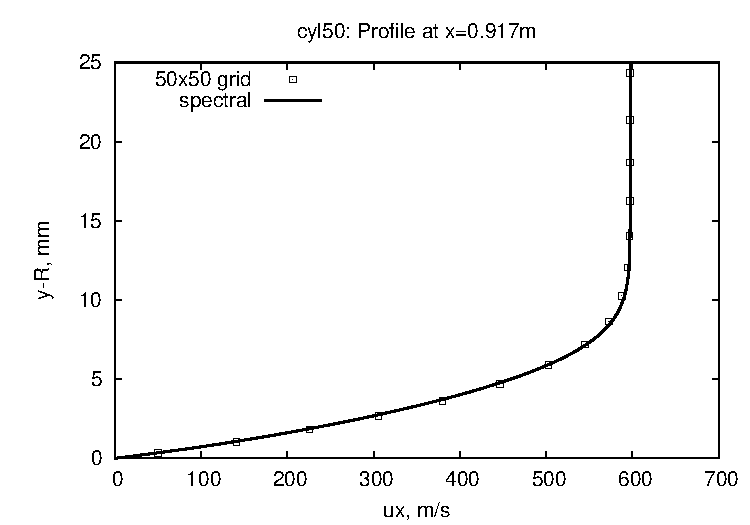
\includegraphics[width=0.5\textwidth]{../2D/axi-cylinder/cyl50_profile_ux.pdf}
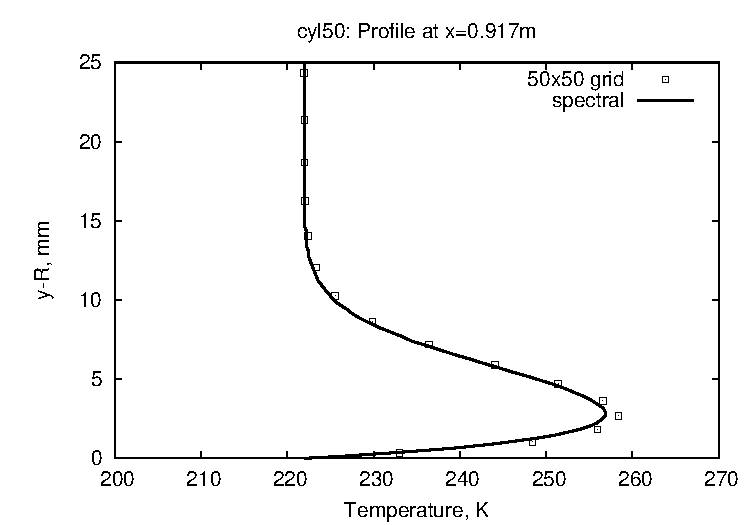
\includegraphics[width=0.5\textwidth]{../2D/axi-cylinder/cyl50_profile_T.pdf}
}
\caption{Velocity and temperature profiles at $x = 0.916$\,m for viscous flow along a cylinder.}
   \label{cyl50-profiles-fig}
\end{figure}

\medskip
This case requires a fairly large computational effort of about 4 hours to reach
a simulation time of 8\,ms.


\newpage
\subsection{Input script (.py)}
\topbar
\lstinputlisting[language={}]{../2D/axi-cylinder/cyl50.py}
\bottombar


\subsection{Shell scripts}
\label{axi-cylinder-sh-files}
\topbar
\lstinputlisting[language={}]{../2D/axi-cylinder/cyl50_run.sh}
\bottombar

\noindent
\topbar
\lstinputlisting[language={}]{../2D/axi-cylinder/cyl50_plot.sh}
\bottombar


\subsection{Notes}
\begin{itemize}
\item None
\end{itemize}



\cleardoublepage
% sharp.tex

\section{Mach 3 flow over a sharp-nosed two-dimensional body}
%
The specifications for this example come from section 5.2
in JD Anderson's Hypersonics book \cite{anderson_89}.
It shows the use of a \texttt{spline} curve as well as being a source
of test data for the Method-of-Characteristics for rotational flow.
Data for the spline points was computed from
$$
\frac{y}{y_e} = -0.008333 + 0.609425 \left( \frac{x}{y_e} \right)
                - 0.092593 \left( \frac{x}{y_e} \right)^2
$$
where $y_e = 1.0$.

\begin{figure}[htbp]
\begin{center}
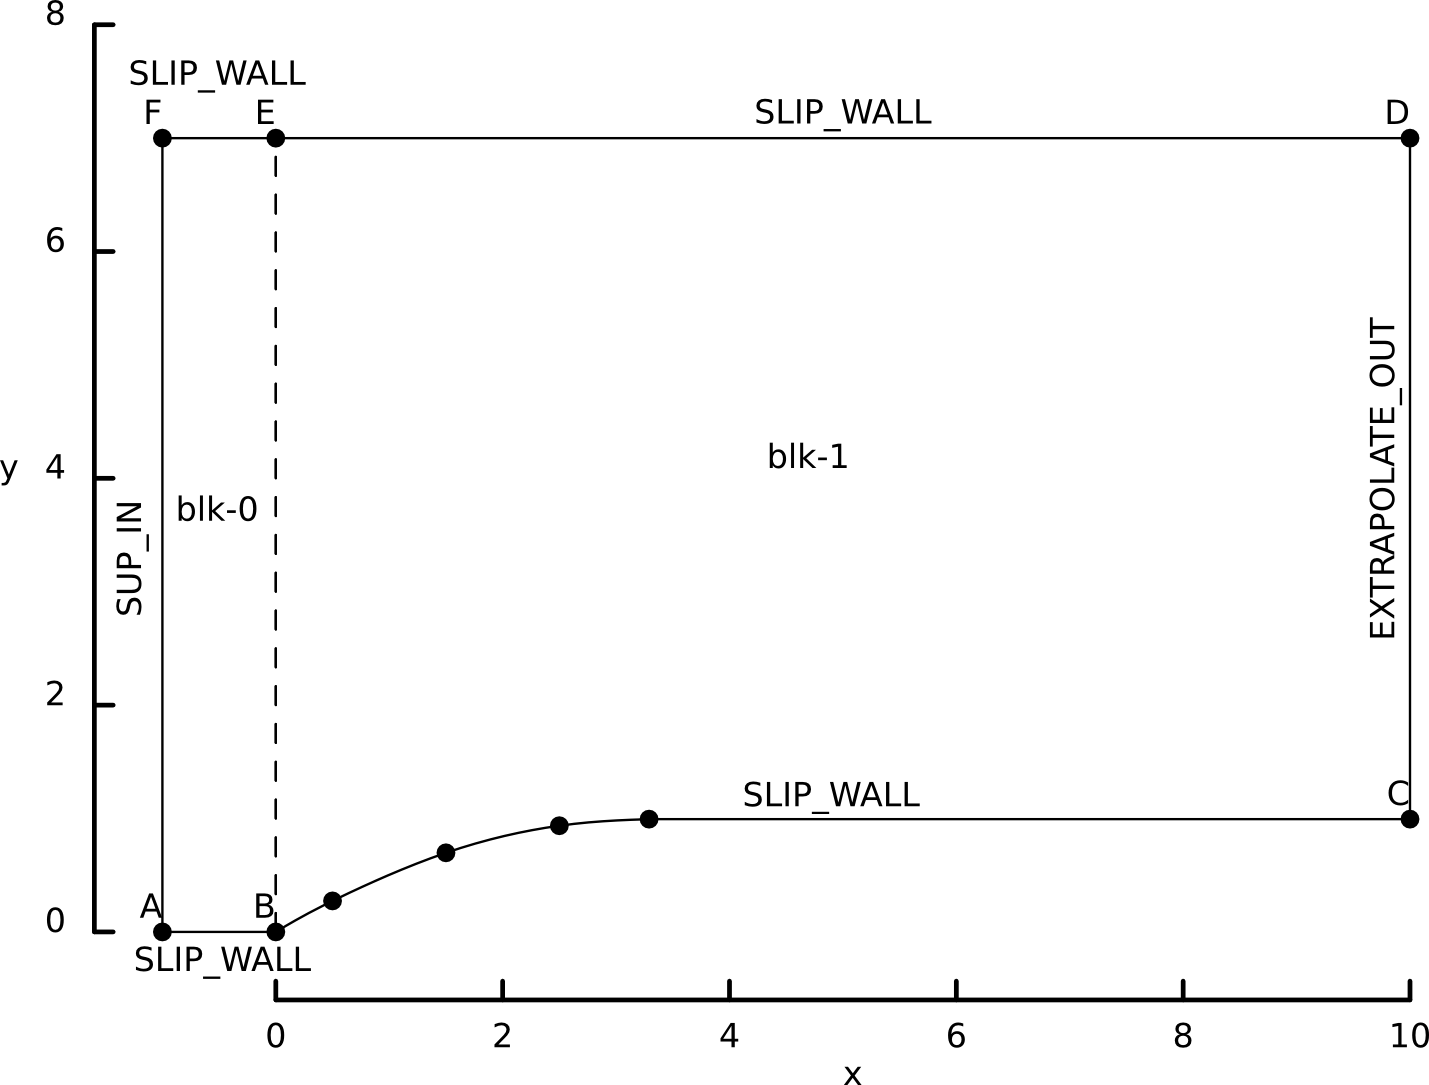
\includegraphics[width=12cm]{../2D/sharp/sharp.png}
\end{center}
\caption{Schematic diagram of the geometry for the sharp body.}
\label{sharp-geometry-fig}
\end{figure}

\begin{figure}[htbp]
\begin{center}
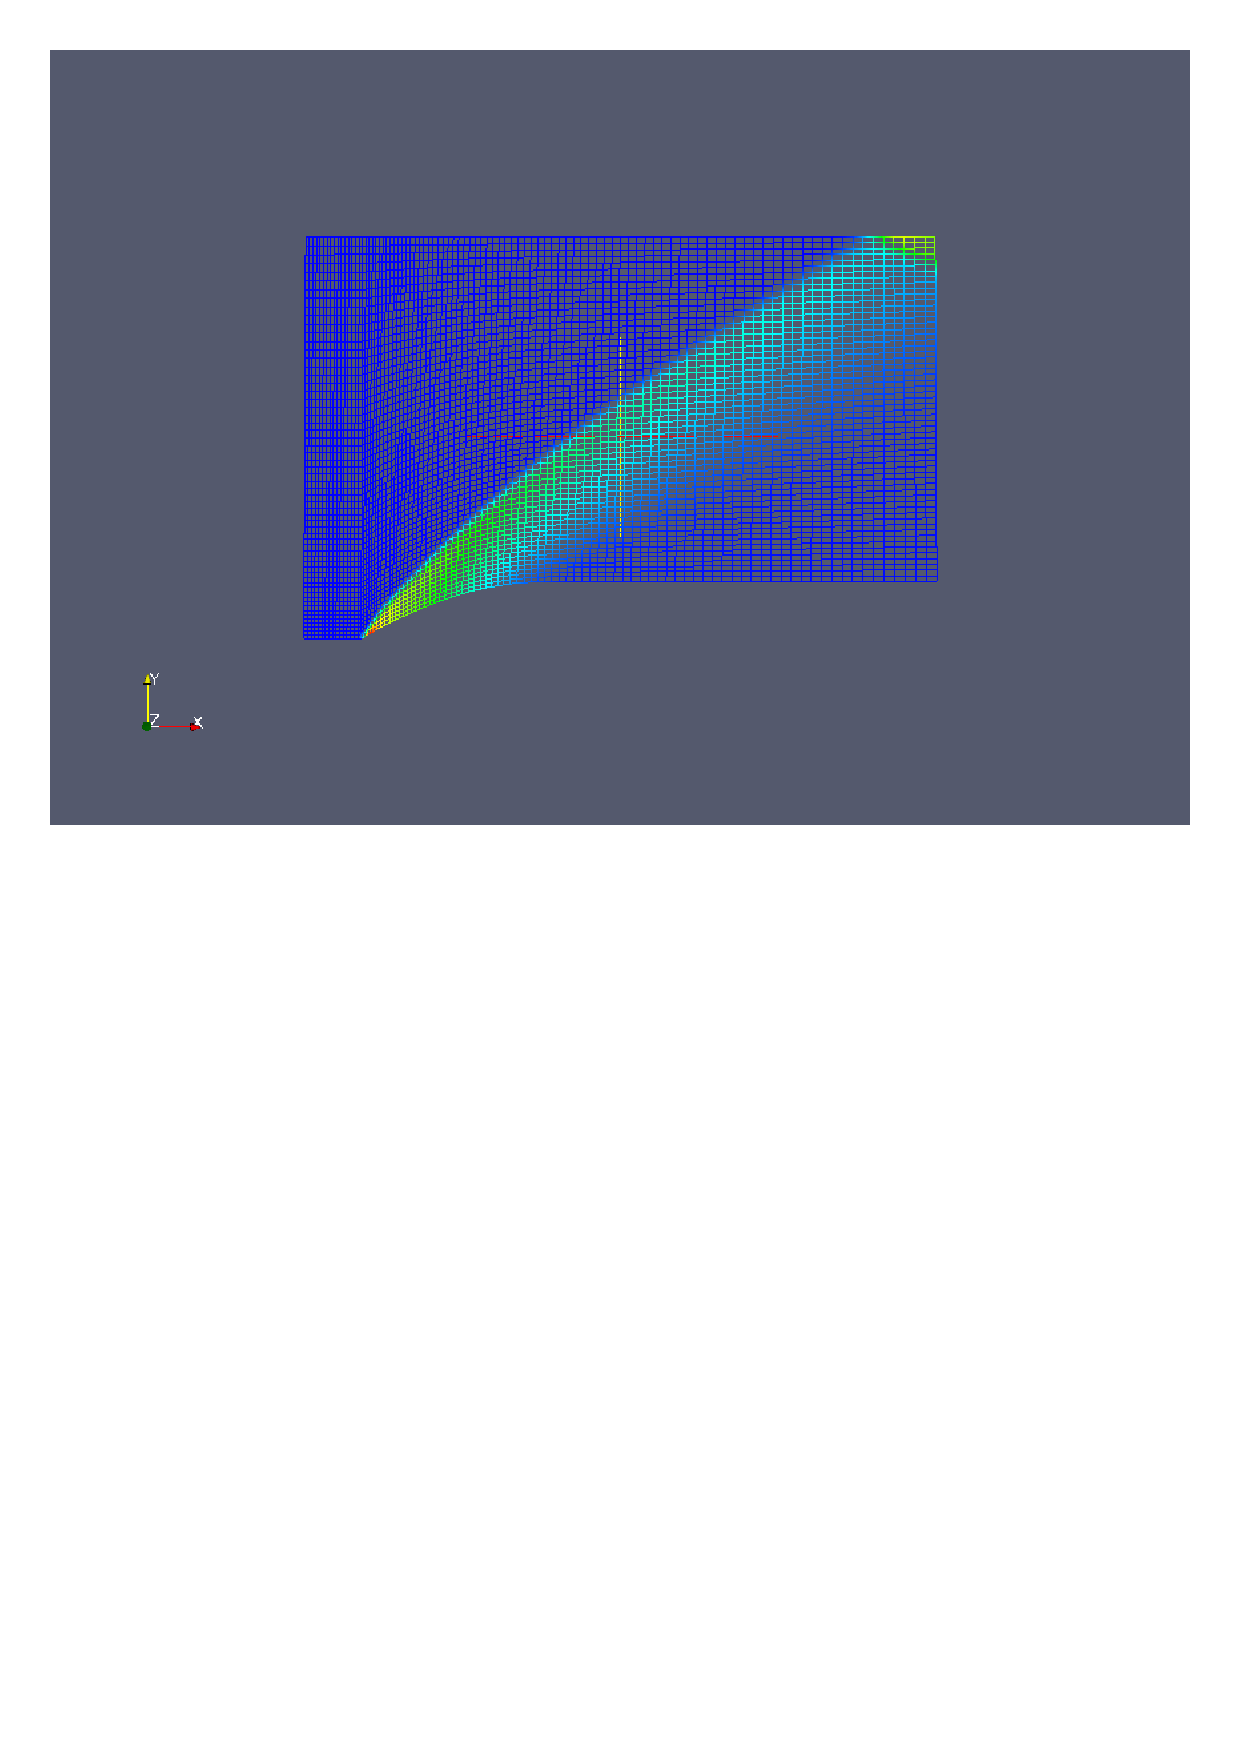
\includegraphics[width=\textwidth, viewport=24 446 570 818]{../2D/sharp/sharp_mesh.pdf}
\end{center}
\caption{Mesh, coloured by pressure, for the sharp body exercise.}
\label{sharp-mesh-fig}
\end{figure}

\begin{figure}[htbp]
\begin{center}
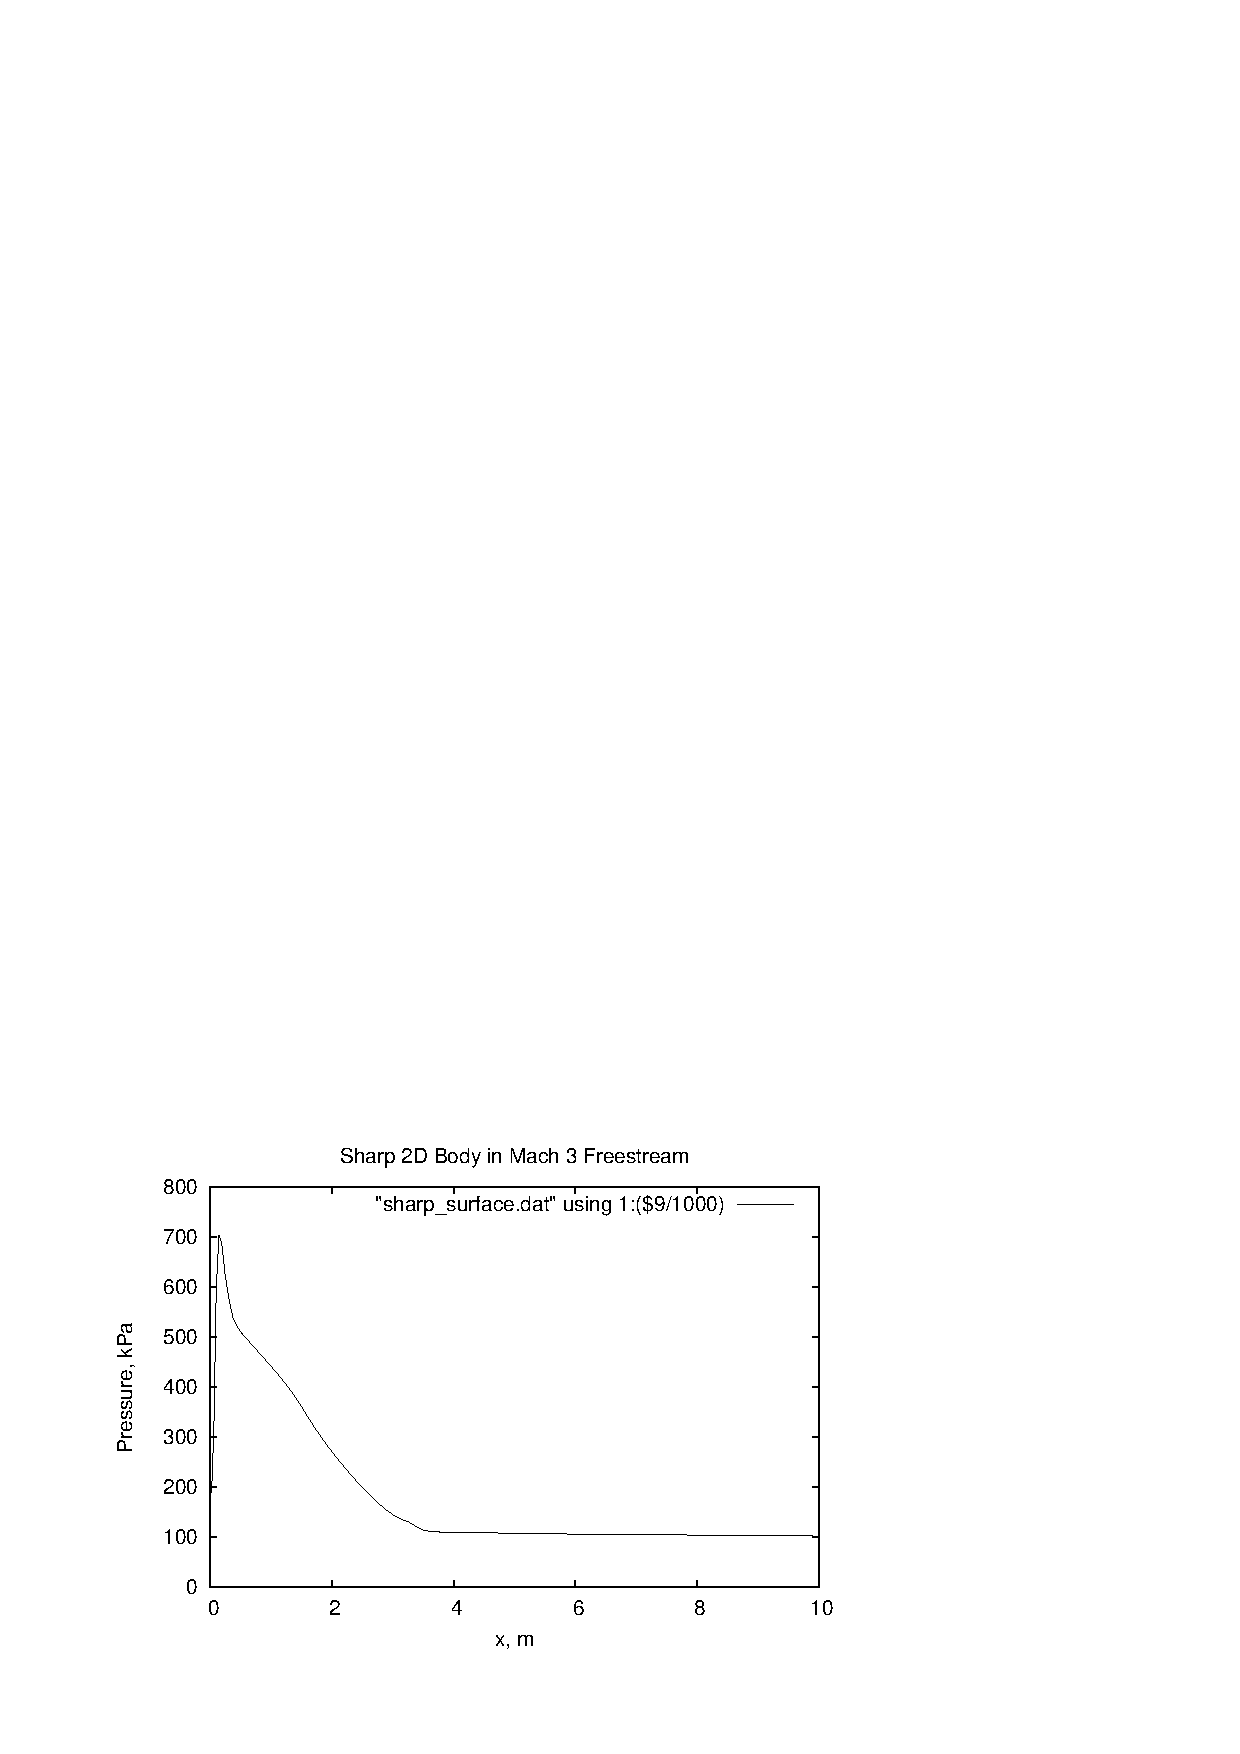
\includegraphics[width=12cm, viewport=55 49 401 292]{../2D/sharp/sharp_surface_p.pdf}
\end{center}
\caption{Pressure data along the body surface.}
\label{sharp-surface-pressure-fig}
\end{figure}

\medskip
The surface pressure (shown in Fig.~\ref{sharp-surface-pressure-fig})
has been extracted from the solution file by \texttt{e3post.py} by selecting the
south-most line of cells of block 1.
The pressure field (Fig.~\ref{sharp-p-fig}) shows the curved shock clearly.

\begin{figure}[htbp]
\begin{center}
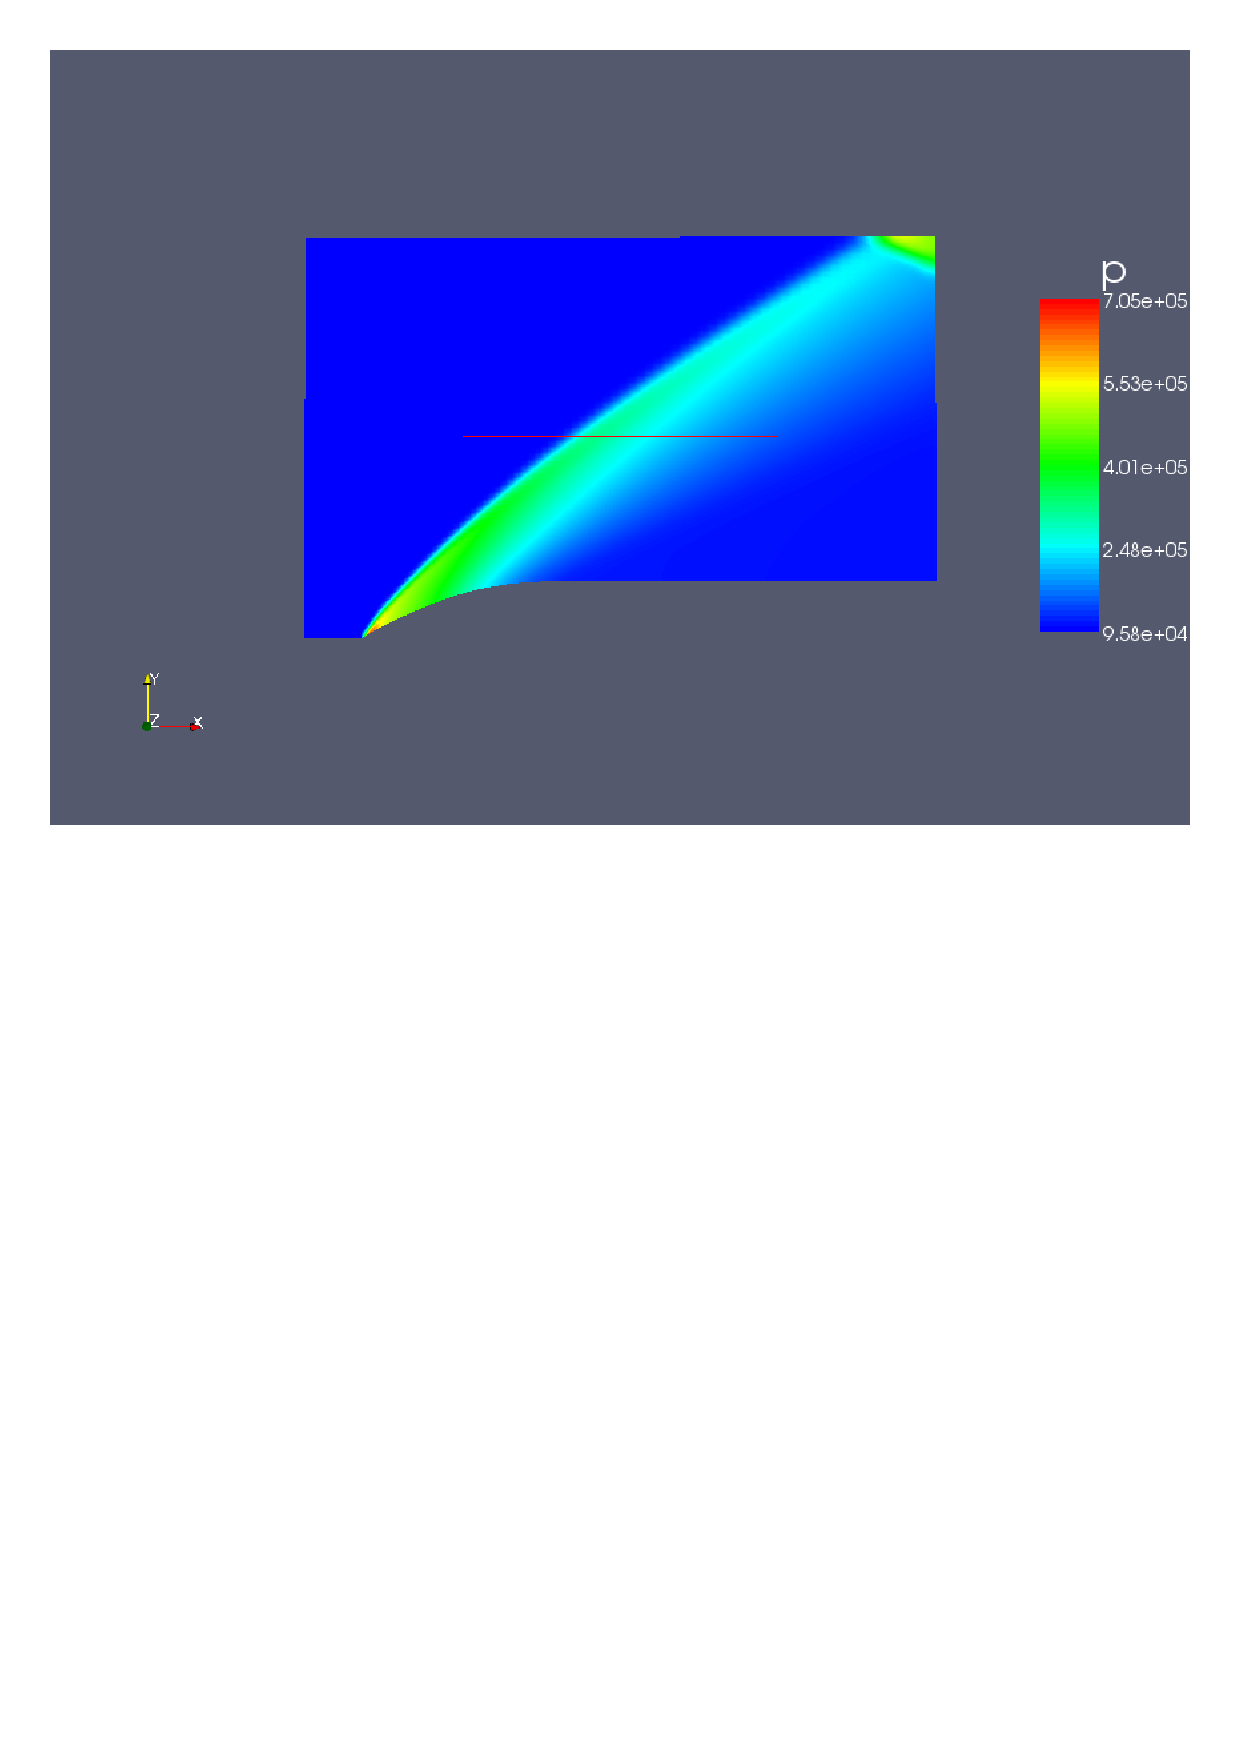
\includegraphics[width=\textwidth, viewport=24 446 570 818]{../2D/sharp/sharp_p.pdf}
\end{center}
\caption{The pressure field for flow over a sharp body.
    The data has been transformed from cells to points in Paraview.
    Note that the shock reflects from the upper boundary,
    which has a SLIP\_WALL boundary condition by default.}
\label{sharp-p-fig}
\end{figure}

\newpage

\subsection{Input script (.py)}
\index{univariate function!RobertsClusterFunction!example of use}
\index{geometric element!Spline!example of use}
\topbar
\lstinputlisting[language={}]{../2D/sharp/sharp.py}
\bottombar


\subsection{Shell scripts}
\label{sharp-sh-files}
\topbar
\lstinputlisting[language={}]{../2D/sharp/sharp_prep.sh}
\bottombar

\noindent
\topbar
\lstinputlisting[language={}]{../2D/sharp/sharp_run.sh}
\bottombar

\noindent
\topbar
\lstinputlisting[language={}]{../2D/sharp/sharp_post.sh}
\bottombar

\subsection{Notes}
\begin{itemize}
\item For mbcns2, this simulation reached a final time of 15\,ms in 1801 steps and,
  on a Pentium-M 1.73\,Ghz system, taking 2\,min, 48\,s of CPU time.
\item For Eilmer3, this simulation required 5\,min, 22\,sec on a single core of 
  a Pentium 1.6\,GHz processor.
  It reached the same time of 15\,ms in 1838 steps.
  As of September 2008, we clearly have some optimisation to do.
\end{itemize}

\cleardoublepage
% sharp-pyfun.tex

\section{Sharp-nosed 2D body -- PyFun version}
%
This is the same flow specifications as for the previous example
but we directly use the functional form of the sharp body as supplied
by Ref.\,\cite{anderson_89}.
$$
\frac{y}{y_e} = -0.008333 + 0.609425 \left( \frac{x}{y_e} \right)
                - 0.092593 \left( \frac{x}{y_e} \right)^2
$$
where $y_e = 1.0$.
In the input script, the path is defined as a \texttt{PyFunctionPath} object that
receives a function \texttt{xypath}.
The function \texttt{xypath} accepts a parameter value $0.0 \le t \le 1.0$ and returns a 
corresponding point along the path as the Python tuple $(x(t), y(t), z(t))$.
Note that it is \textit{not} a \texttt{Vector} object as most of the other geometry objects expect.

\bigskip
\subsection{Input script (.py)}\index{geometric element!PyFunctionPath!example of use}
\topbar
\lstinputlisting[language={}]{../2D/sharp-pyfun/sharp.py}
\bottombar

\subsection{Notes on using Python for the input script}
\begin{itemize}
 \item The script runs in the context set up by the \texttt{e3prep.py} program.
  This means that data elements such as \texttt{gdata} are available for manipulation
  by the user's script.
 \item Comments can be used in the script as a form of documentation on the simulation.
 \item We can get intermediate results printed as the script is processed.  
  This is useful for debugging and for documentation of the situation.
 \item It is often convenient to set up small functions that get passed as arguments to
  other functions.  For example, the function \texttt{y} (brought over from the previous
  simulation) is passed into \texttt{xypath} which is, in turn, passed in to PyFunctionPath
  to construct a Path element. 
\end{itemize}

\cleardoublepage
% blunt_wedge.tex

\newpage
\section{Hypersonic flow of ideal air over a blunt wedge}
\label{blunt-wedge-sec}
%
This example is a partial solution to the CFD exercise for
the MECH4470 class in 2004.
Because the original specification was given in nondimensional form,
an arbitrary 10\,mm nose radius has been selected for the
inviscid simulation.
This is also a reasonable size for a possible wind tunnel experiment.
The free-stream condition was specified as having a Mach number of 5
and the gas was specified as ideal air.
Choosing particular values of $p_{\infty} = 100$\,kPa, $T_{\infty} = 100$\,K, 
lead to a free-stream velocity of $u_{\infty} = 1002$\,m/s and 
a dynamic pressure of $q_{\infty} = 1.75$\,MPa.

\begin{figure}[htbp]
\begin{center}
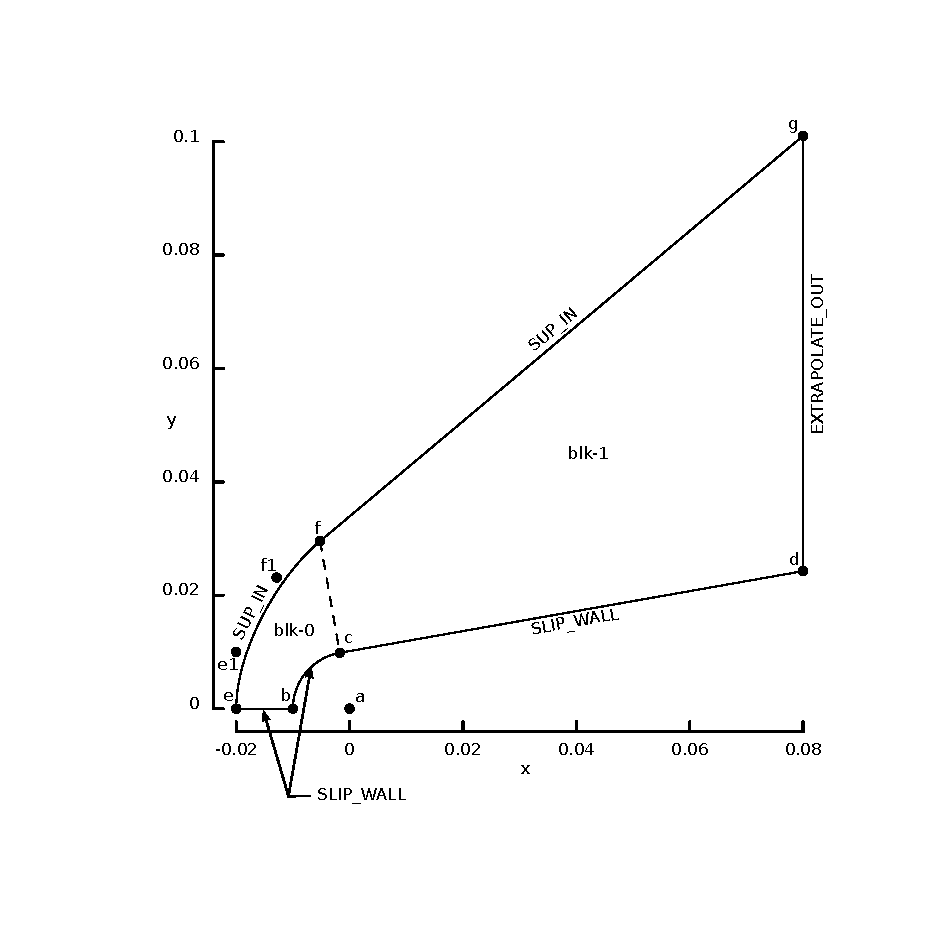
\includegraphics[width=10cm,viewport=77 67 398 398,clip=true]{../2D/blunt-wedge/bw-layout.pdf}
\end{center}
\caption{Schematic diagram of the geometry for the blunted 10 degree wedge.}
\label{bw-geometry-fig}
\end{figure}

\begin{figure}[htbp]
\begin{center}
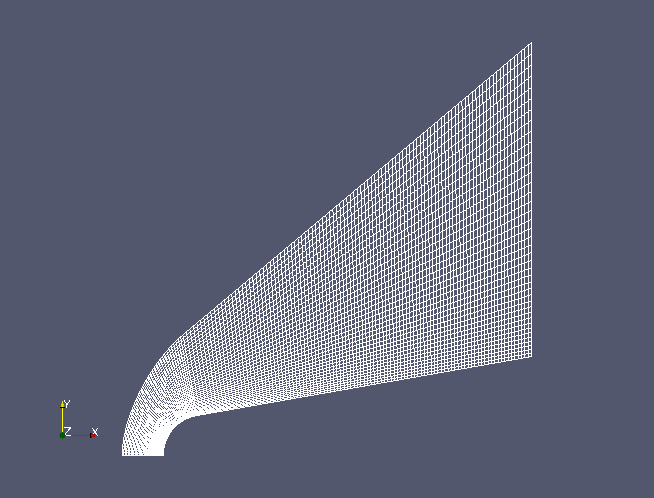
\includegraphics[width=0.8\textwidth]{../2D/blunt-wedge/bw-mesh.png}
\end{center}
\caption{Mesh for the blunt wedge exercise.}
\label{bw-mesh-fig}
\end{figure}

\medskip
The simulation is started with low-pressure conditions throughout the flow
domain and free-stream conditions applied to the inflow boundary
(the west boundary of blk-0 and the north boundary of blk-1).
The flow data is allowed to evolve until $t_{final} = 399\,\mu$s,
which corresponds to a particle of the free-stream travelling 40 nose radii.
The axial force (shown in Fig.\ref{bw-xforce-fig}) is seen to settle to 
a value of 28590\,N in that time.
This corresponds to a drag coefficient of 0.674.

\begin{figure}[htbp]
\begin{center}
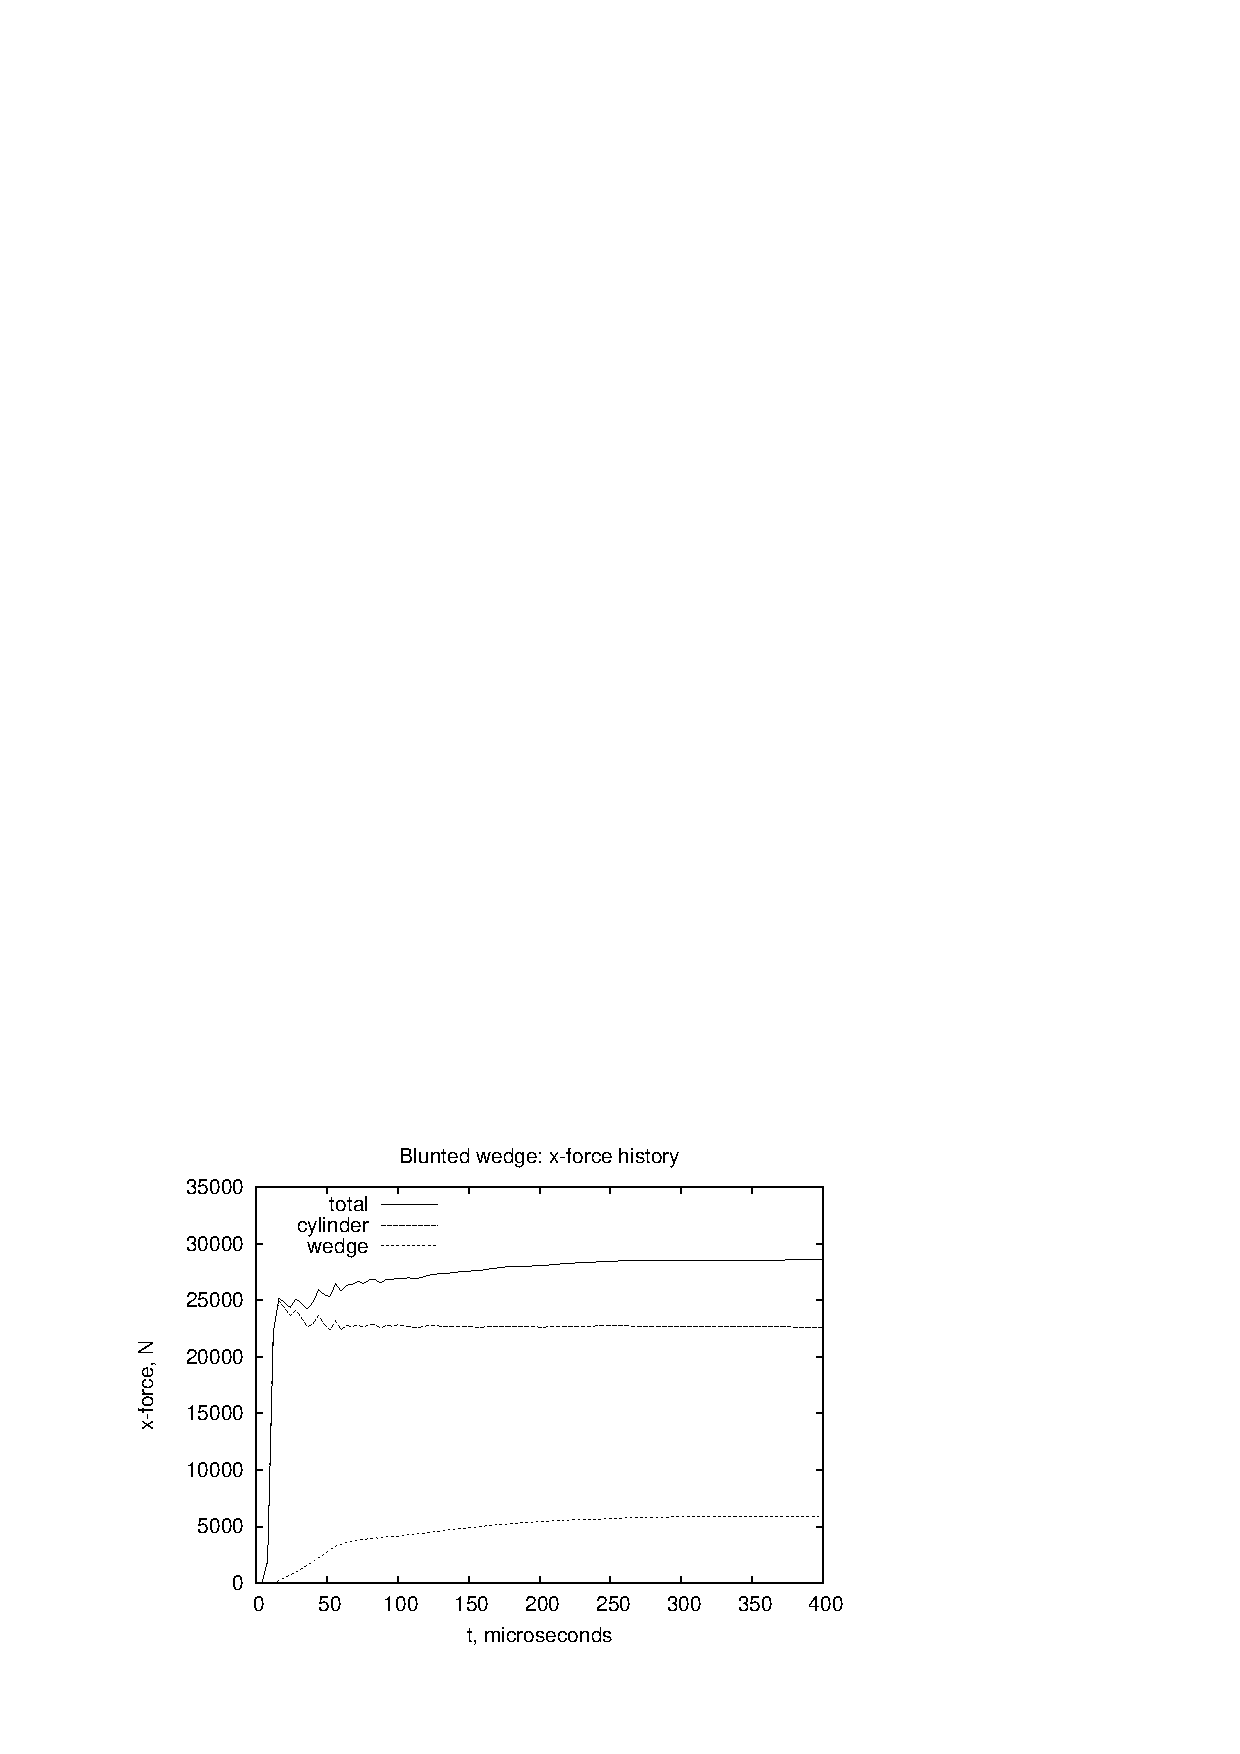
\includegraphics[width=12cm,viewport=66 52 404 292,clip=true]{../2D/blunt-wedge/bw_xforce.pdf}
\end{center}
\caption{History of the axial forces for the blunt-wedge exercise.}
\label{bw-xforce-fig}
\end{figure}

\begin{figure}[htbp]
\begin{center}
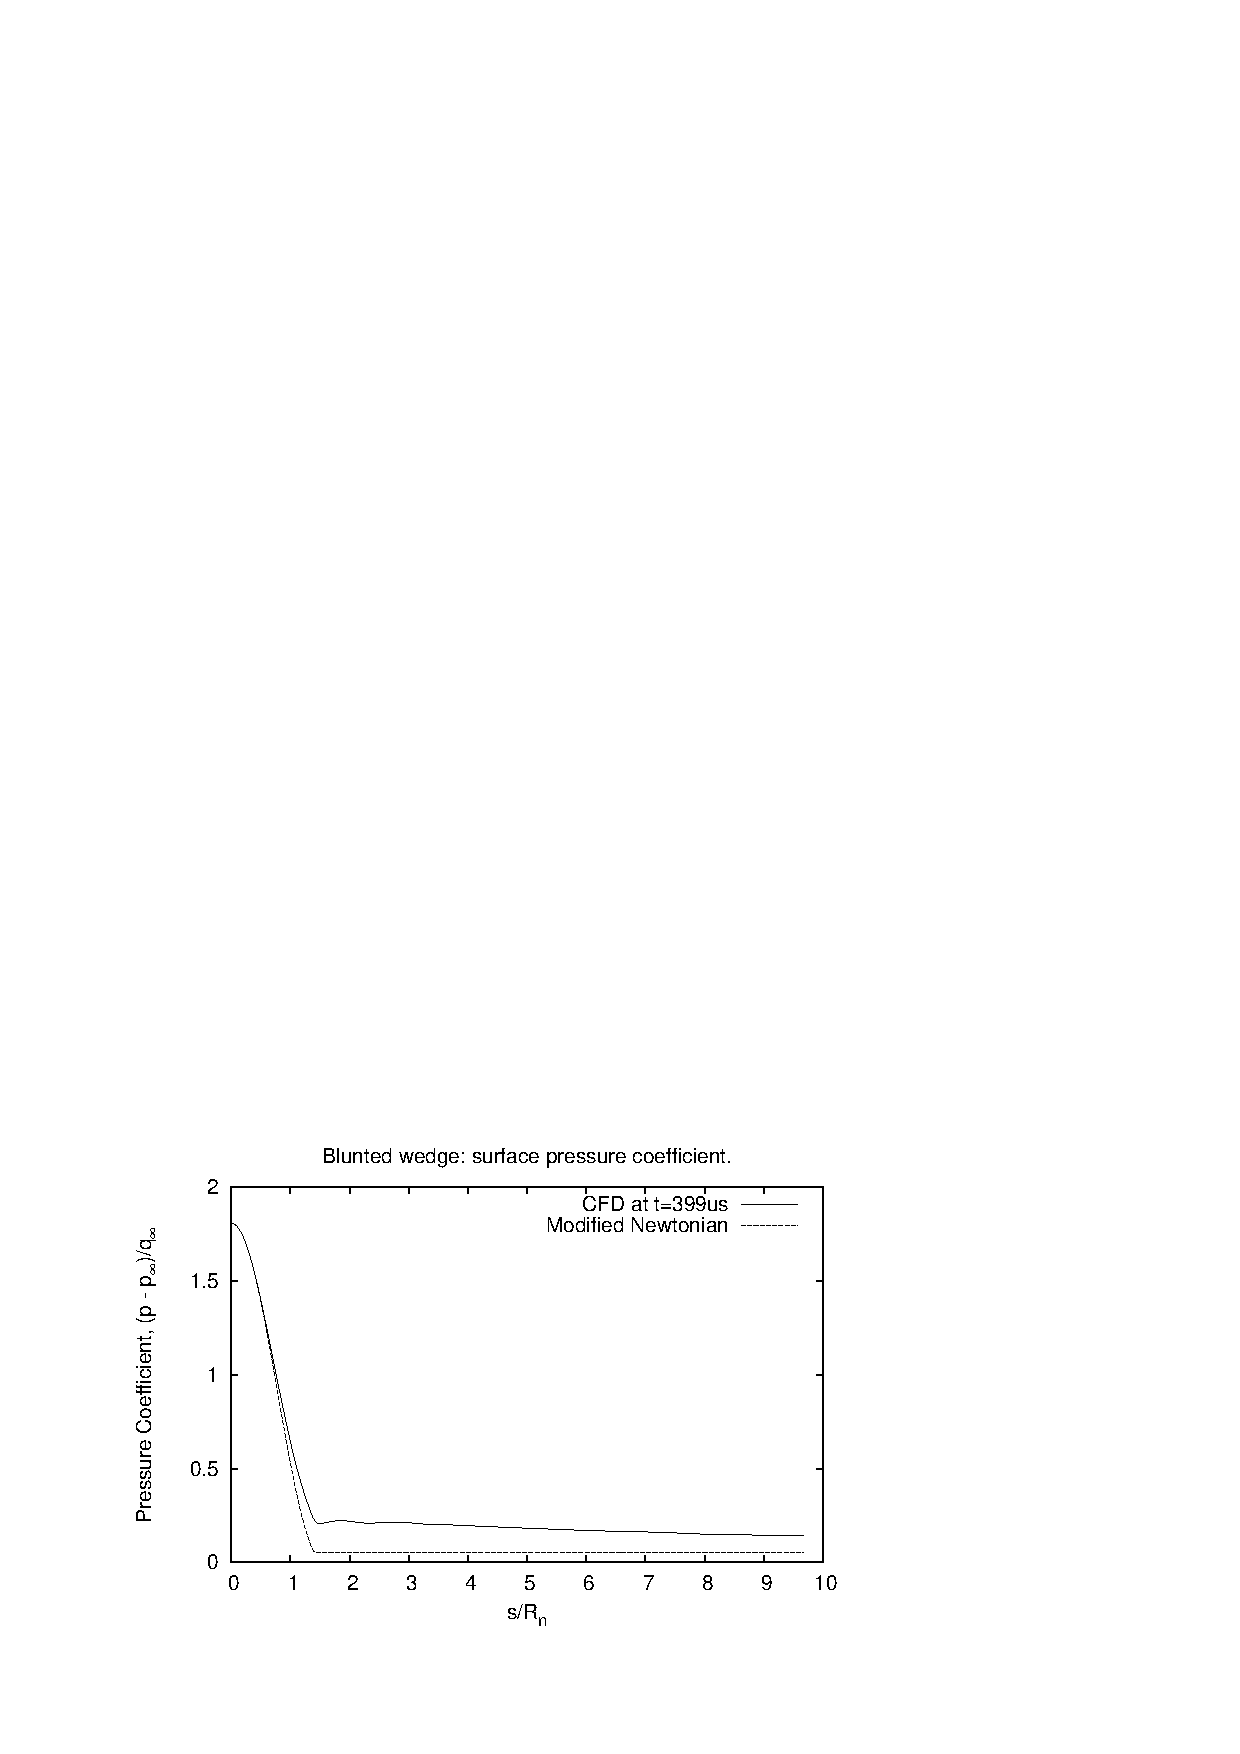
\includegraphics[width=12cm,viewport=64 61 401 291,clip=true]{../2D/blunt-wedge/bw_surface_pressure.pdf}
\end{center}
\caption{Surface pressure coefficient data for the blunt-wedge exercise.}
\label{bw-surface-pressure-fig}
\end{figure}

\medskip
The surface pressure (shown normalised in Fig.~\ref{bw-surface-pressure-fig})
has been extracted from the solution file by \texttt{e3post.py} by selecting the
east-most line of cells of the first block and the south-most line of cells
of the second block.
The selected data is filtered by an Awk script to produce the normalised data
(and the Newtonian reference data) as plotted.

\begin{figure}[htbp]
\begin{center}
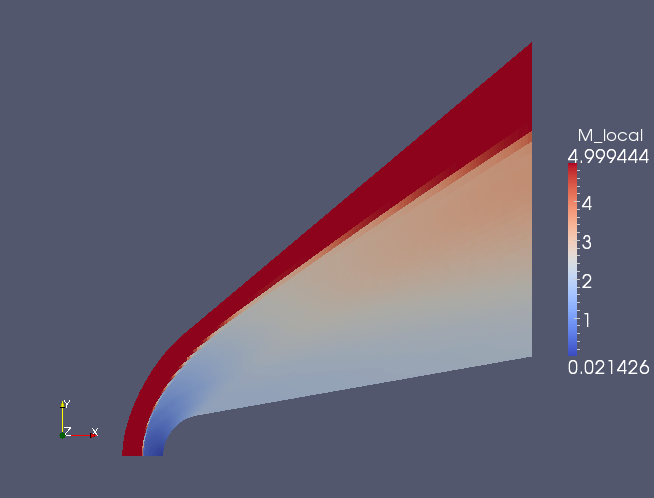
\includegraphics[width=0.8\textwidth]{../2D/blunt-wedge/bw-Mach-field.png}
\end{center}
\caption{Mach number data for the blunt-wedge exercise.}
\label{bw-Mach-fig}
\end{figure}

\newpage

\subsection{Input script (.py)}\index{xforce\_list!example of use}
\topbar
\lstinputlisting[language={}]{../2D/blunt-wedge/bw.py}
\bottombar

\newpage
\subsection{Shell scripts}
\label{bw-sh-files}
\topbar
\lstinputlisting[language={}]{../2D/blunt-wedge/bw_prep.sh}
\bottombar

\noindent
\topbar
\lstinputlisting[language={}]{../2D/blunt-wedge/bw_run.sh}
\bottombar

\noindent
\topbar
\lstinputlisting[language={}]{../2D/blunt-wedge/bw_post.sh}
\bottombar

\newpage
\subsection{Notes}
\begin{itemize}
\item This simulation reaches a final time of 399\,$\mu$s.
      For \texttt{mbcns2} on an Intel Pentium-M 1.73\,Ghz system, this took 6\,min, 39\,s of CPU time
      for 3722 steps.
      However, for \texttt{Eilmer3} on an Intel E2140 1.6Ghz system it now takes 15\,m, 23\,s
      for 3759 steps.
\item Selection of the \texttt{e3shared.log} file showing some x-force data
      as written during the simulation.
      Pressure and viscous forces are written separately.
      Note that the lines are written with several items separated by spaces and the
      format is mostly self-documenting.
      The only extra bit of information is that BNDY values are 0, 1, 2 and 3 for
      boundaries NORTH, EAST, SOUTH and WEST, respectively.
\footnotesize
\begin{verbatim}
Step=    420 t= 2.747e-05 dt= 9.100e-08 WC=102.0 WCtFT=991.8 WCtMS=1112.3
CFL_min = 1.862345e-03, CFL_max = 4.958796e-01, dt_allow = 9.100331e-08
Smallest CFL_max so far = 3.381457e-02 at t = 1.000000e-07
 dt[0]=9.100331e-08 dt[1]=1.500771e-07
There are 2 active blocks.
RESIDUAL mass block 0 max: 4.899825e-02 at (-0.00280173,0.0146712,0)
RESIDUAL energy block 0 max: 5.025321e-02 at (-0.00280173,0.0146712,0)
RESIDUAL mass block 1 max: 1.656031e-01 at (0.0254165,0.0185377,0)
RESIDUAL energy block 1 max: 4.834703e-01 at (0.0262722,0.0181336,0)
RESIDUAL mass global max: 1.656031e-01 step 420 time 2.74667e-05
RESIDUAL energy global max: 4.834703e-01 step 420 time 2.74667e-05
XFORCE: TIME 2.801336e-05 BLOCK 0 BNDY 1 FX_P 2.415181e+04 FX_V 2.204480e+00 
XFORCE: TIME 2.801336e-05 BLOCK 1 BNDY 2 FX_P 9.973561e+02 FX_V 9.133770e+00 
\end{verbatim}
\normalsize

\item Awk filter for extracting the x-force data from the simulation log file.
      Note that there are two pattern-action rules, one for each block.
      \lstinputlisting[language={}]{../2D/blunt-wedge/xforce.awk}
\item Awk filter for normalising the surface pressure data.
      \lstinputlisting[language={}]{../2D/blunt-wedge/surface_pressure.awk}
\end{itemize}

\cleardoublepage
% bar-476.tex
% See the folder on flat-faced cylinders

\section{Pressure on a flat-faced cylinder}
\label{bar-476-sec}
%
This example models the bar gauge type of pressure sensor 
as used in the expansion-tube facilities.
It also shows the application of a multiple-block grid to
describe the flow domain (Figure\,\ref{bar-geometry-fig}) around a flat-faced
cylinder whose axis is aligned with the free-stream flow direction.
The free-stream Mach number is 4.76 to match one of the higher Mach number
conditions reported in Ref.\cite{kendall_1959a}.

\begin{figure}[htbp]
\begin{center}
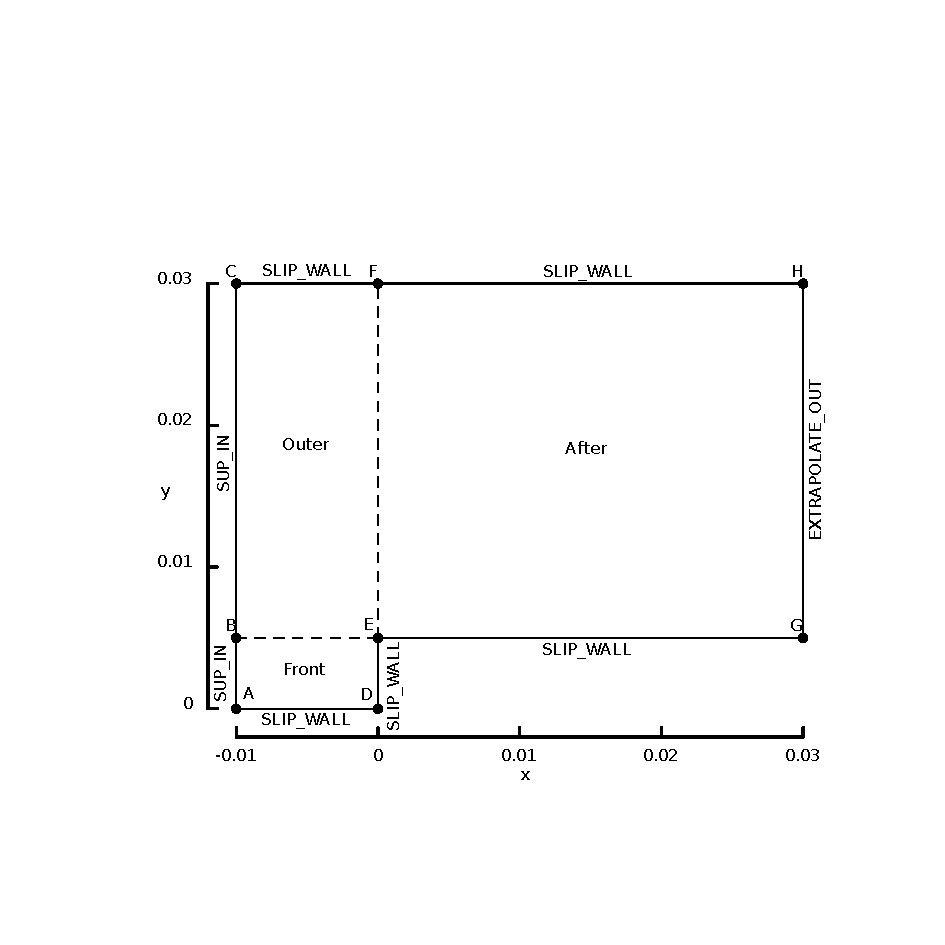
\includegraphics[width=12cm,viewport=75 78 397 328,clip=true]{../2D/bar-476/bar-layout.pdf}
\end{center}
\caption{Schematic diagram of the full flow domain around the flat-faced cylinder.}
\label{bar-geometry-fig}
\end{figure}

The simulation is started with low pressure stationary gas throughout
the domain and the inflow conditions are applied to the west boundaries
of blocks ``Front'' and ``Outer''.
After allowing 50\,$\mu$s for the flow to reach steady state, 
the pressure distribution throughout the domain is shown in
Fig.\,\ref{bar-pressure-mach-fig}.
The stand-off distance was determined by searching
for the pressure jump along the row of cells adjacent to the centreline.
See the \texttt{locate\_shock.awk} script below.
If the trigger for the pressure jump is 200\,kPa, the stand-off distance is 2.815\,mm but, 
if we use a level of 1.5\,MPa, the estimated stand-off distance is 2.756\,mm.
The difference is about 70\% of one cell width. 

\begin{figure}[htbp]
\mbox{
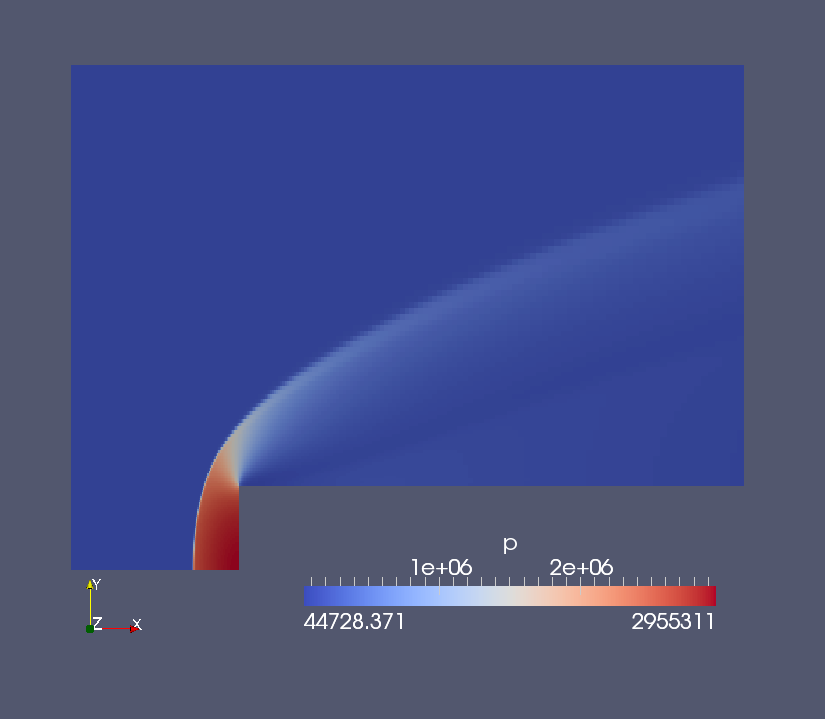
\includegraphics[width=0.5\textwidth]{../2D/bar-476/bar-p-field.png}
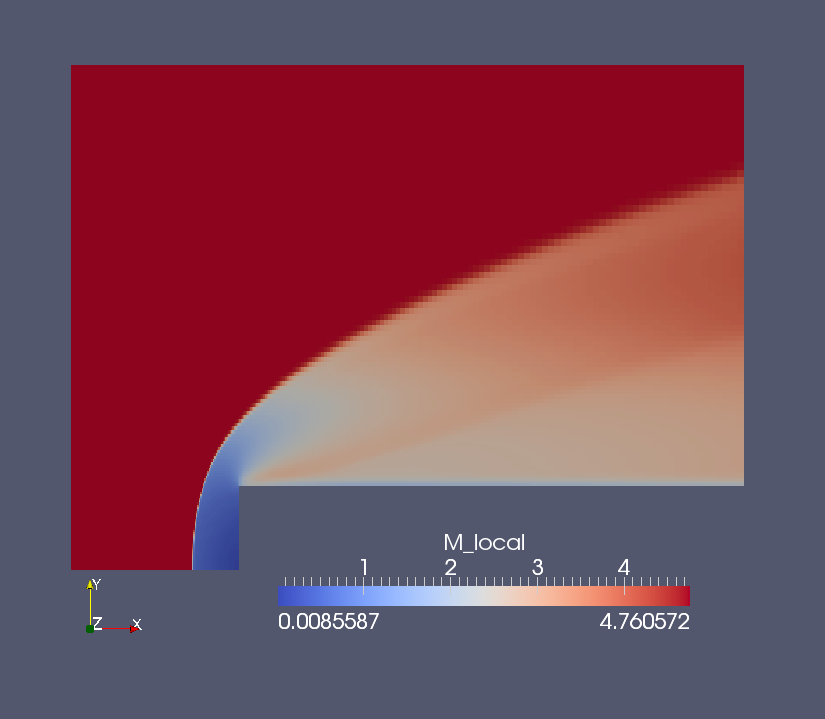
\includegraphics[width=0.5\textwidth]{../2D/bar-476/bar-Mach-field.png}
}
\caption{Pressure and Mach number within the flow domain at 50\,$\mu$s.}
\label{bar-pressure-mach-fig}
\end{figure}

Figure~\ref{bar-pressure-profile-fig} shows the distribution of pressure
across the face of the cylinder.  
The simulation data agrees closely with Kendall's measurements 
except in the region the sharp corner where there is inadequate resolution
and an absence of viscous effects in the simulation.

\begin{figure}[htbp]
\begin{center}
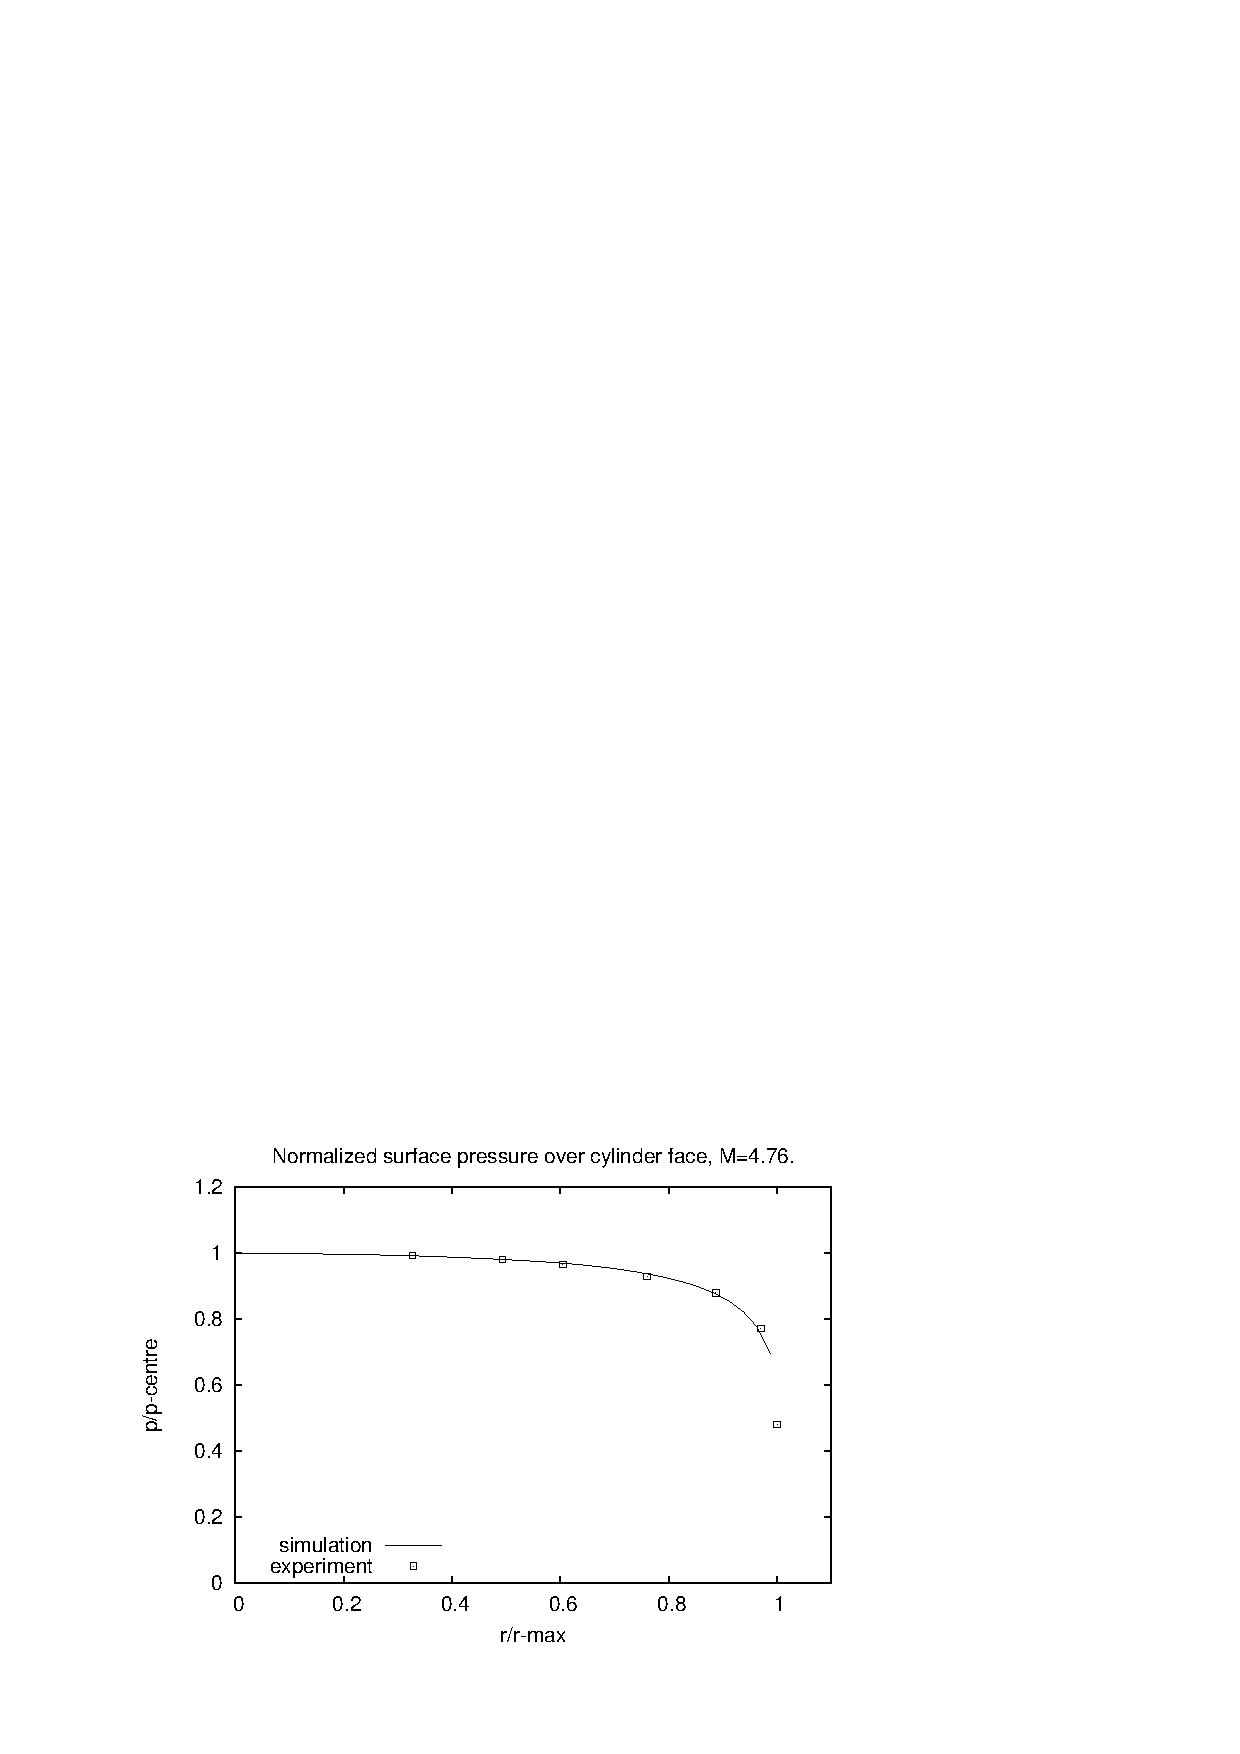
\includegraphics[width=10cm,viewport=68 53 400 291,clip=true]{../2D/bar-476/bar_norm_p.pdf}
\end{center}
\caption{Normalised pressure across the face of the cylinder
         compared with experimental measurements\,\cite{kendall_1959a}.}
\label{bar-pressure-profile-fig}
\end{figure}

\newpage
\subsection{Input script (.py)}
\topbar
\lstinputlisting[language={}]{../2D/bar-476/bar.py}
\bottombar

\newpage
\subsection{Shell scripts}
\label{bar-sh-files}
\topbar
\lstinputlisting[language={}]{../2D/bar-476/prepare_simulation.sh}
\bottombar

\noindent
\topbar
\lstinputlisting[language={}]{../2D/bar-476/run_simulation.sh}
\bottombar

\noindent
\topbar
\lstinputlisting[language={}]{../2D/bar-476/post_simulation.sh}
\bottombar

\newpage
\subsection{Awk scripts}
\label{bar-awk-files}
\topbar
\lstinputlisting[language={}]{../2D/bar-476/normalize.awk}
\bottombar

\noindent
\topbar
\lstinputlisting[language={}]{../2D/bar-476/locate_shock.awk}
\bottombar


\subsection{Notes}
\begin{itemize}
\item The \texttt{mbcns2} version of this simulation 
      reaches a final time of 50\,$\mu$s in 2932 steps and,
      on a Pentium-M 1.73\,Ghz system, this takes 19\,min, 27\,s of CPU time.
      This is equivalent to 17.8\,$\mu$s per cell per predictor-corrector
      time step.
\item The \texttt{Eilmer3} simulation takes 2929 steps and 19\,min, 6\,s on 
      an Intel Core 2 Duo E8400 at 3GHz.
      We have some optimization to do...
\end{itemize}

\cleardoublepage
% back-nozzle.tex

\newpage
\section{Flow through a conical nozzle}
\label{back-nozzle-sec}
%
Good quality experimental data for wall pressure distribution in a conical
nozzle with a circular-arc throat profile and a 15$^o$ divergent section
is available in Ref.\,\cite{back_etal_1965a}.
In the original experiment, the flow of air through the facility 
was allowed to reach steady state and static pressures were measured 
at a large number of points along the nozzle wall.

% In contrast, the present simulation is transient with just the transonic 
% plus supersonic parts of the flow field reaching steady state.
% Fixed 2014

Figure\,\ref{back-geometry-fig} shows the outline of the simulated flow
domain which is set up to approximate the largest subsonic area ratio
used in the experiment.
A short subsonic section upstream of the throat is included, along with
the conical supersonic expansion where the pressure measurements were made.
Note that the geometric calculation of the tangent arcs is done within the
input script.
This makes use of Python, beyond just being an input format, and allows the
specification to be fully parametric.
Although the parametric description makes the initial setup of the script 
a bit more complex than absolutely necessary, 
it does make the running of the simulation for other radii of curvature 
very simple.

\begin{figure}[htbp]
\begin{center}
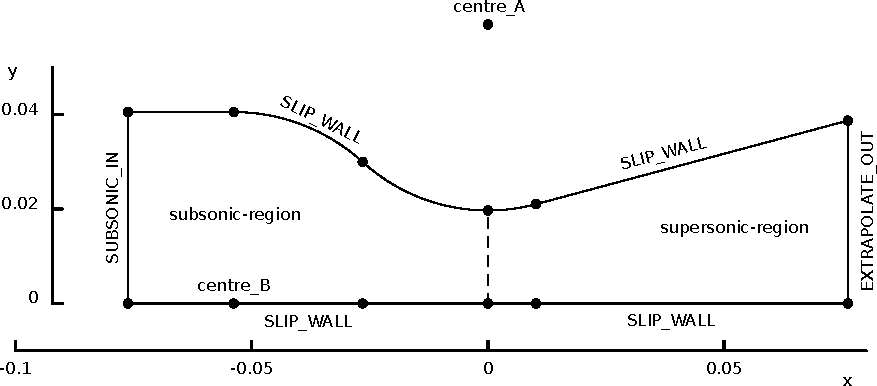
\includegraphics[width=\textwidth]{../2D/back-nozzle/back-layout.pdf}
\end{center}
\caption{Schematic diagram of the full flow domain for the duct and conical nozzle.}
\label{back-geometry-fig}
\end{figure}

% The relatively long upstream part of the simulated tube provides the gas 
% through an unsteady expansion from zero speed and pressure of 500\,kPa 
% (state 4) up to a small Mach number (state 3).
% These state labels refer to the those for 
% the hypothetical shock tube problem in which 
% state 1 is the initial low-pressure condition, 
% state 4 is the initial high-pressure condition,
% state 2 is the post-shock condition of the low-pressure gas,
% and state 3 is the expanded high-pressure gas condition.

% Along the $C_+$ characteristic connecting states 4 and 3, 
% the Riemann invariant can be written as 
% $$
%     J_+ = u + \frac{2 a}{\gamma - 1} ~~~,
% $$
% and so the relation between states 4 and 3 can be written as
% $$
%     \frac{a_4}{a_3} = 1 + \frac{\gamma - 1}{2} M_3 ~~~.
% $$
% Because the unsteady expansion is isentropic and $a = \sqrt{\gamma R T}$,
% the pressure ratio can be written as
% $$
%     \frac{p_4}{p_3} = \left[ 1 + \frac{\gamma - 1}{2} M_3 
%                       \right]^{2 \gamma / (\gamma - 1)}
% $$
% which gives a specific pressure ratio of $p_4/p_3 = 1.2102$.
% Since the experiment used a steady expansion from a large reservoir
% at stagnation conditions to the equivalent of our state 3, 
% the corresponding stagnation pressure for state 3 is computed from
% $$
%     \frac{p_{03}}{p_3} = \left[ 1 + \frac{\gamma - 1}{2} M_3^2
%                                \right]^{\gamma / (\gamma - 1)} 
% $$
% which gives $p_{03} = 418.7$\,kPa in the current simulation.

Figure\,\ref{back-mesh-fig} shows the mesh, coloured by Mach number 
(once the flow has reached steady state).
Assuming that flow in the subsonic and transonic regions of the nozzle is
steady, the expected Mach number is $M_3 = 0.13812$ for an area ratio of 
$A_3 / A_* = 4.2381$.
This is seen to be consistent with the Mach number colouring in the figure
and is a good test of the \verb!SubsonicInBC! that is applied at the 
upstream boundary.\index{boundary conditions!SubsonicInBC!example of use}

\begin{figure}[htbp]
\begin{center}
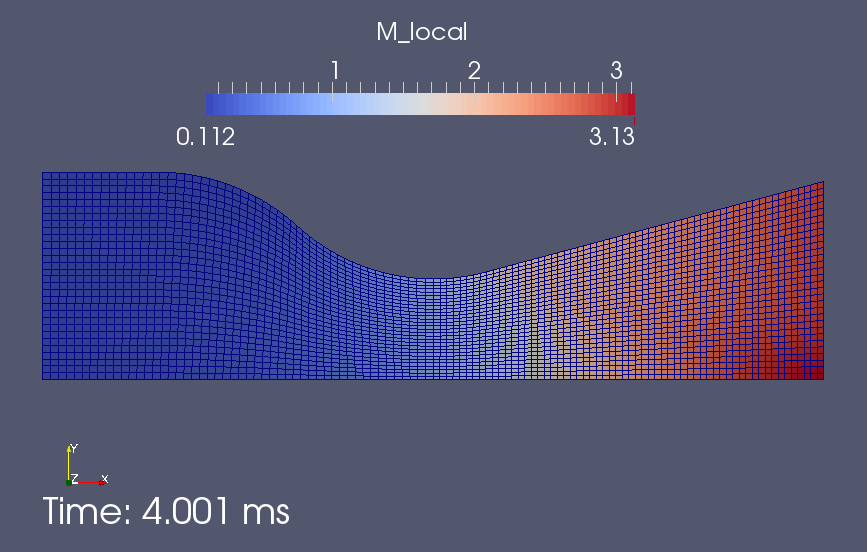
\includegraphics[width=0.8\textwidth]{../2D/back-nozzle/back-mach-field-with-mesh.png}
\end{center}
\caption{Mesh generated for the axisymmetric nozzle simulation, coloured with Mach number.}
\label{back-mesh-fig}
\end{figure}

Figure\,\ref{back-pressure-contours-fig} shows the pressure distribution
throughout the flow domain at $t = 4.0$\,ms, once the flow has settled.
Note that the inflow boundary has the flow stagnation properties specified as its
flow condition but that this condition does not appear in any part of the simulation domain.

\begin{figure}[htbp]
\begin{center}
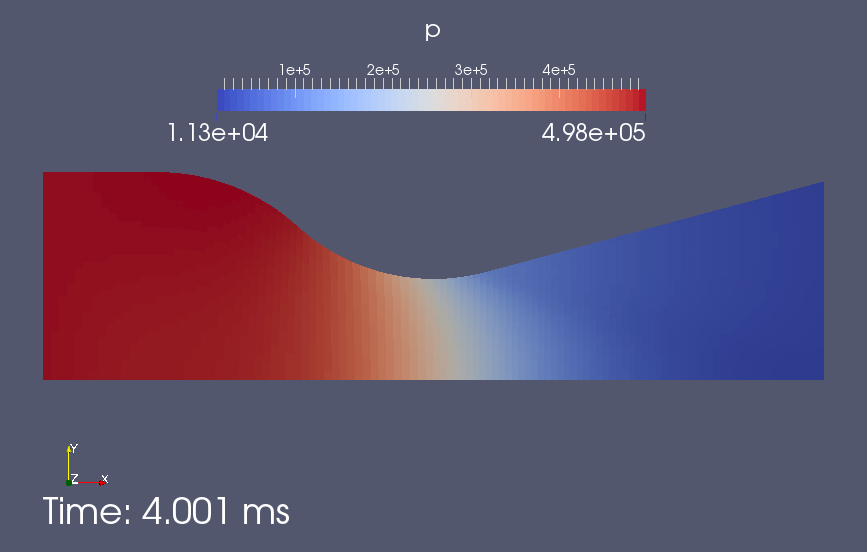
\includegraphics[width=0.8\textwidth]{../2D/back-nozzle/back-p-field.png}
\end{center}
\caption{Pressure contours within the flow domain at 4.0\,ms.}
\label{back-pressure-contours-fig}
\end{figure}

The flow in the nozzle is largely transient as the stagnation conditions drive gas into the domain
but the overall flow becomes steady, as indicated by the histories
shown in Fig.\,\ref{back-transient-fig}.
Because there is little damping to the gas dynamics, small scale oscillations evident in the pressure
history take some to damp out as weak waves bounce around in the subsonic region long after the bulk flow
has approached steady state.
Figure\,\ref{back-profile-fig} shows that the simulation matches the
experimental data closely.

\begin{figure}[htbp]
\begin{center}
\begin{tabular}{cc}
(a) & (b) \\
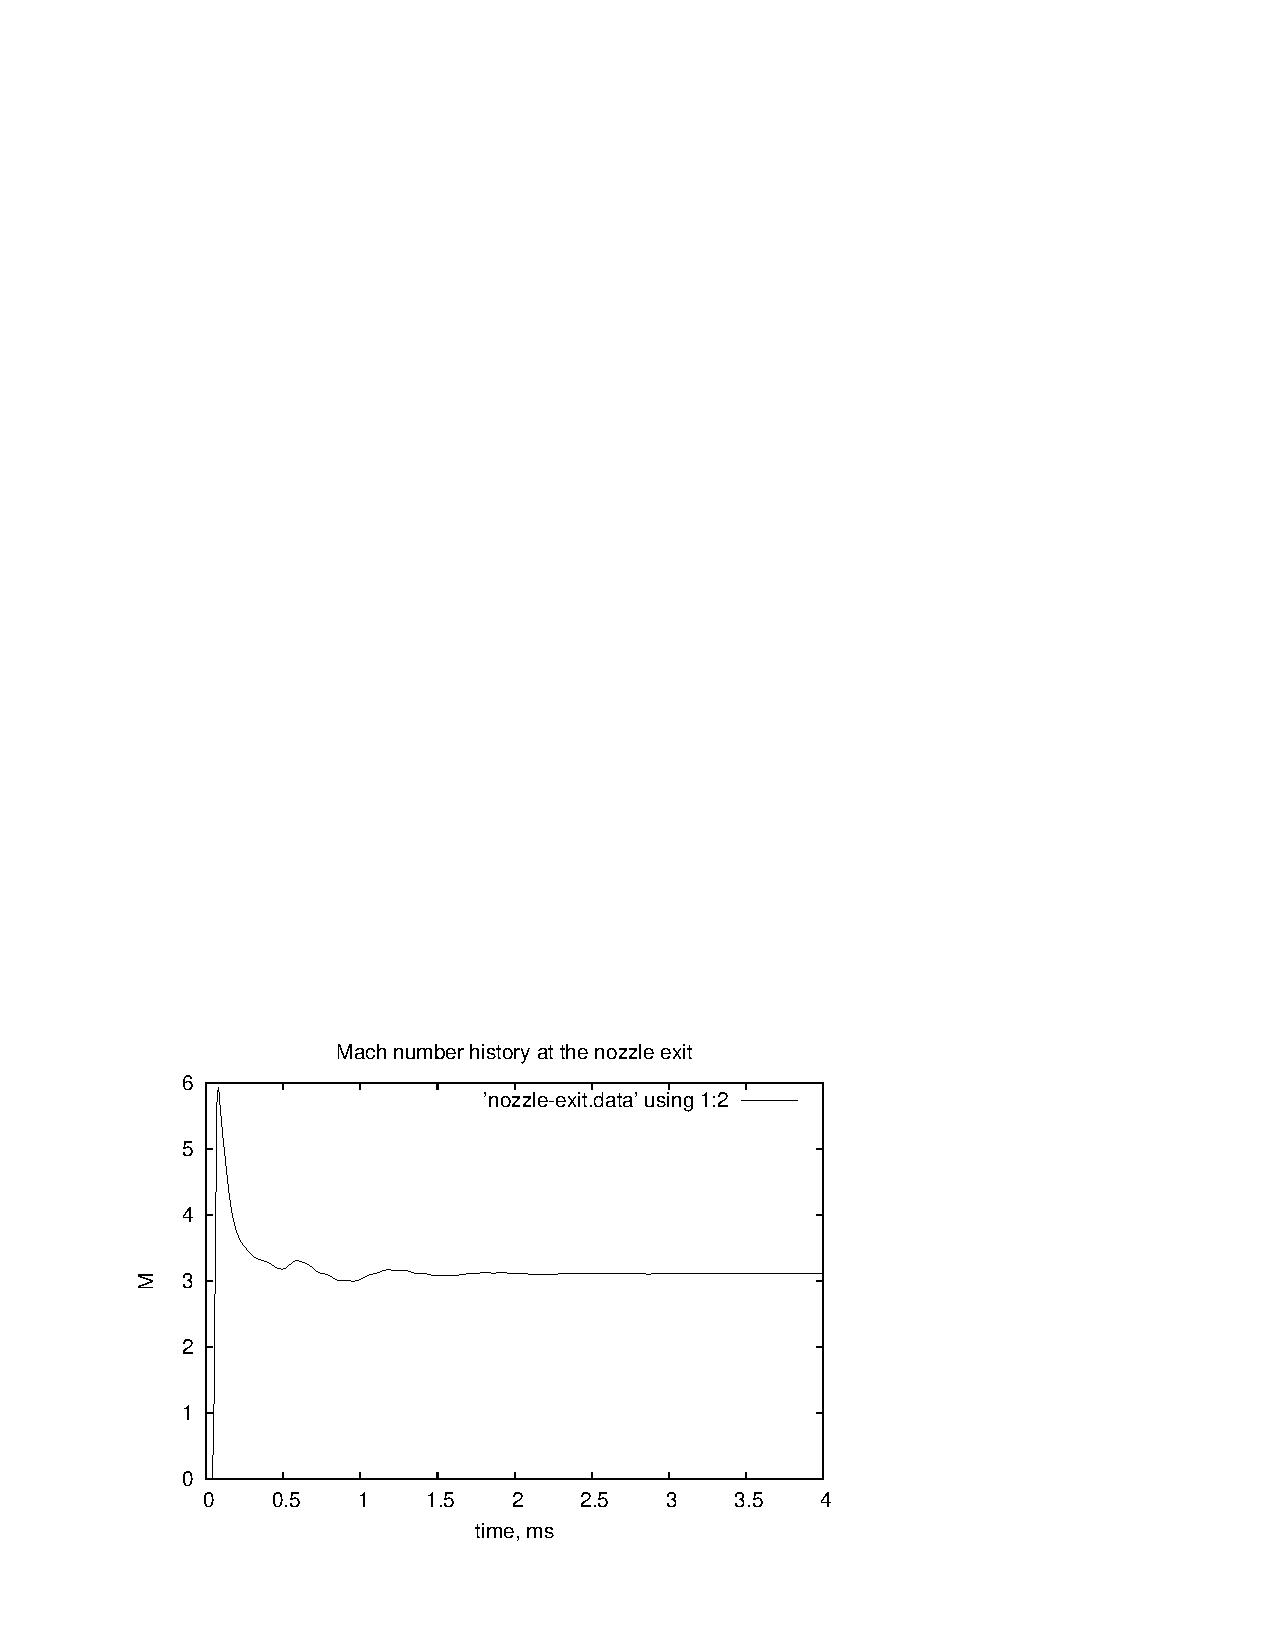
\includegraphics[width=0.5\textwidth]{../2D/back-nozzle/back_history_M.pdf} &
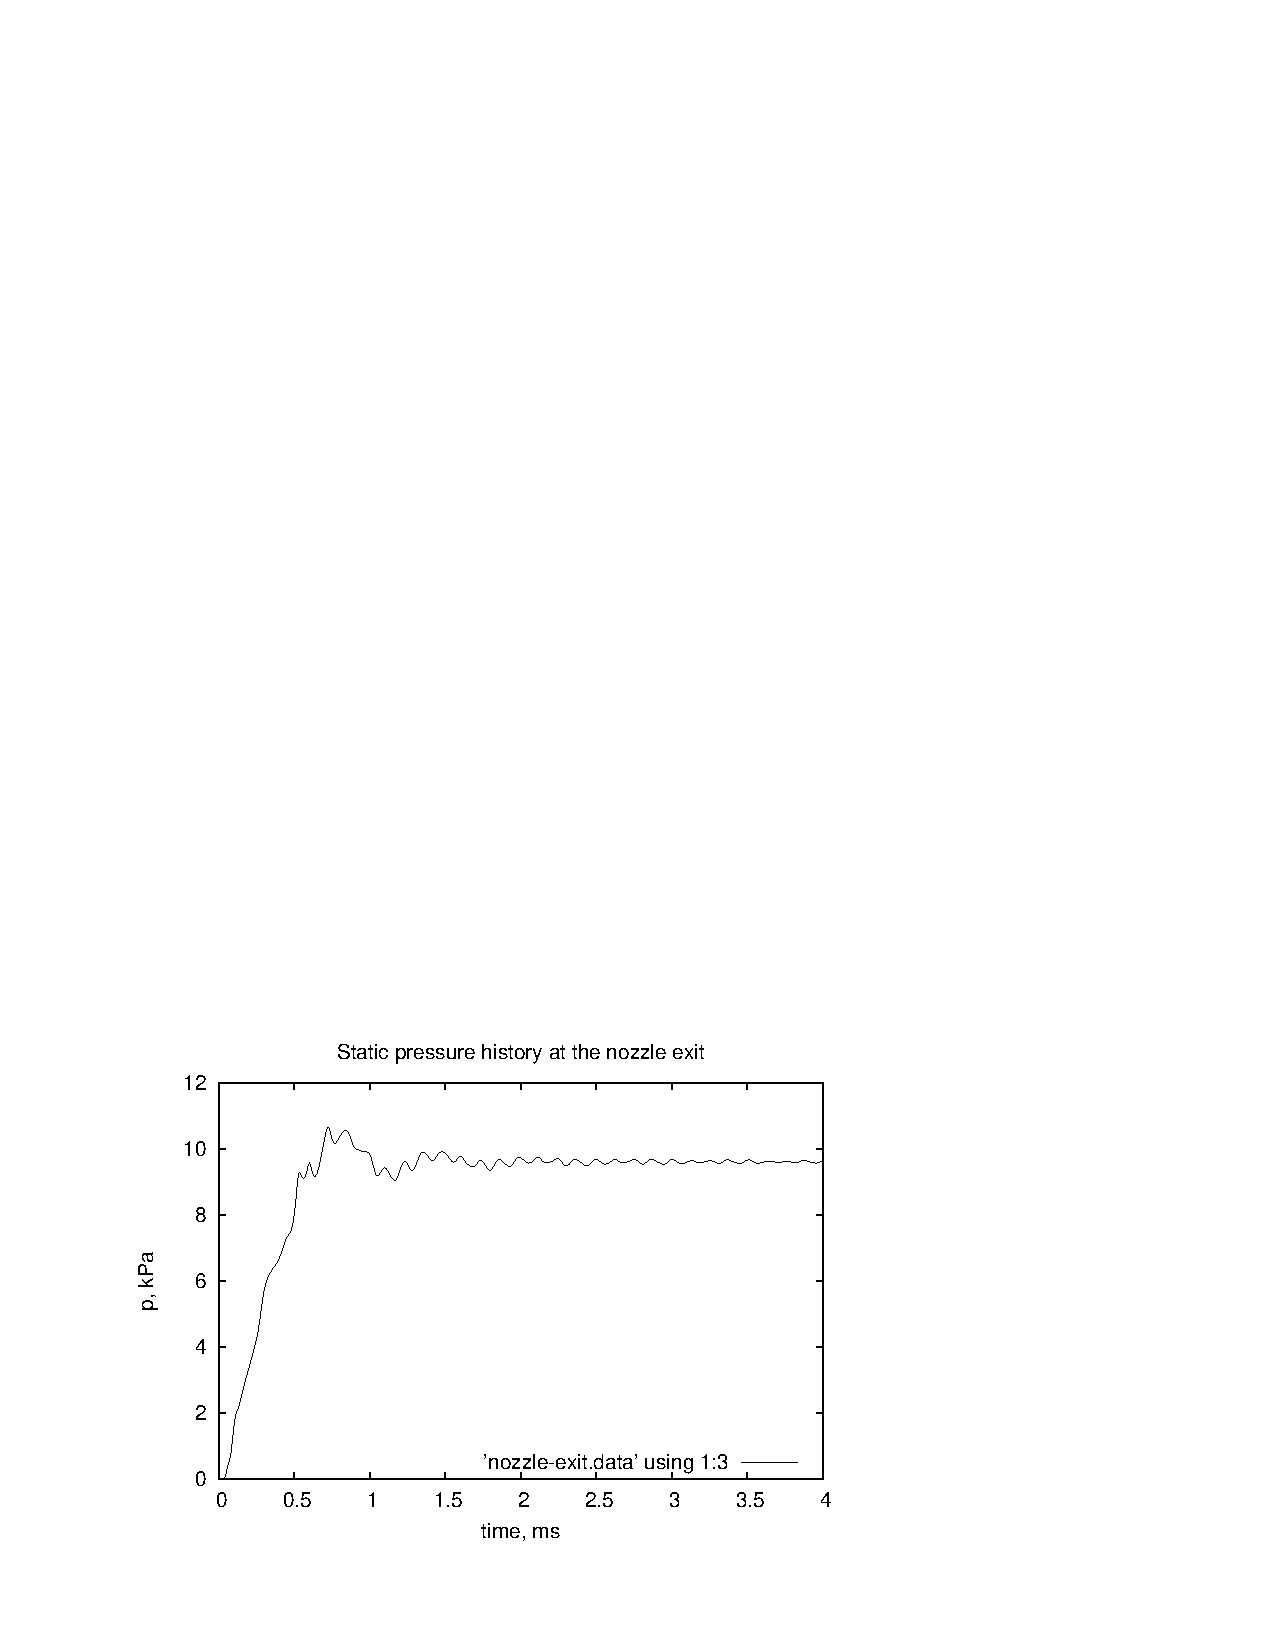
\includegraphics[width=0.5\textwidth]{../2D/back-nozzle/back_history_p.pdf}
\end{tabular}
\end{center}
\caption{Development of the flow at a ``history point'' near
         the centre of the exit plane:
         (a) Mach number;
         (b) static pressure.}
\label{back-transient-fig}
\end{figure}

\begin{figure}[htbp]
\begin{center}
\begin{tabular}{cc}
(a) & (b) \\
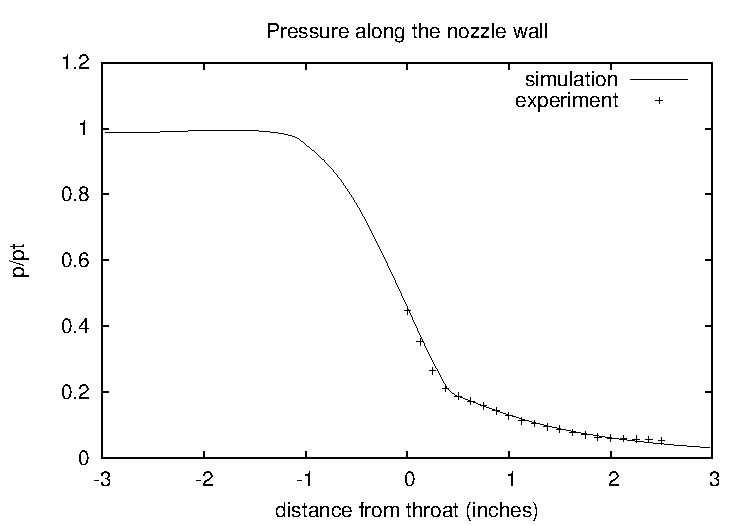
\includegraphics[width=0.5\textwidth]{../2D/back-nozzle/back_profile_whole.pdf} &
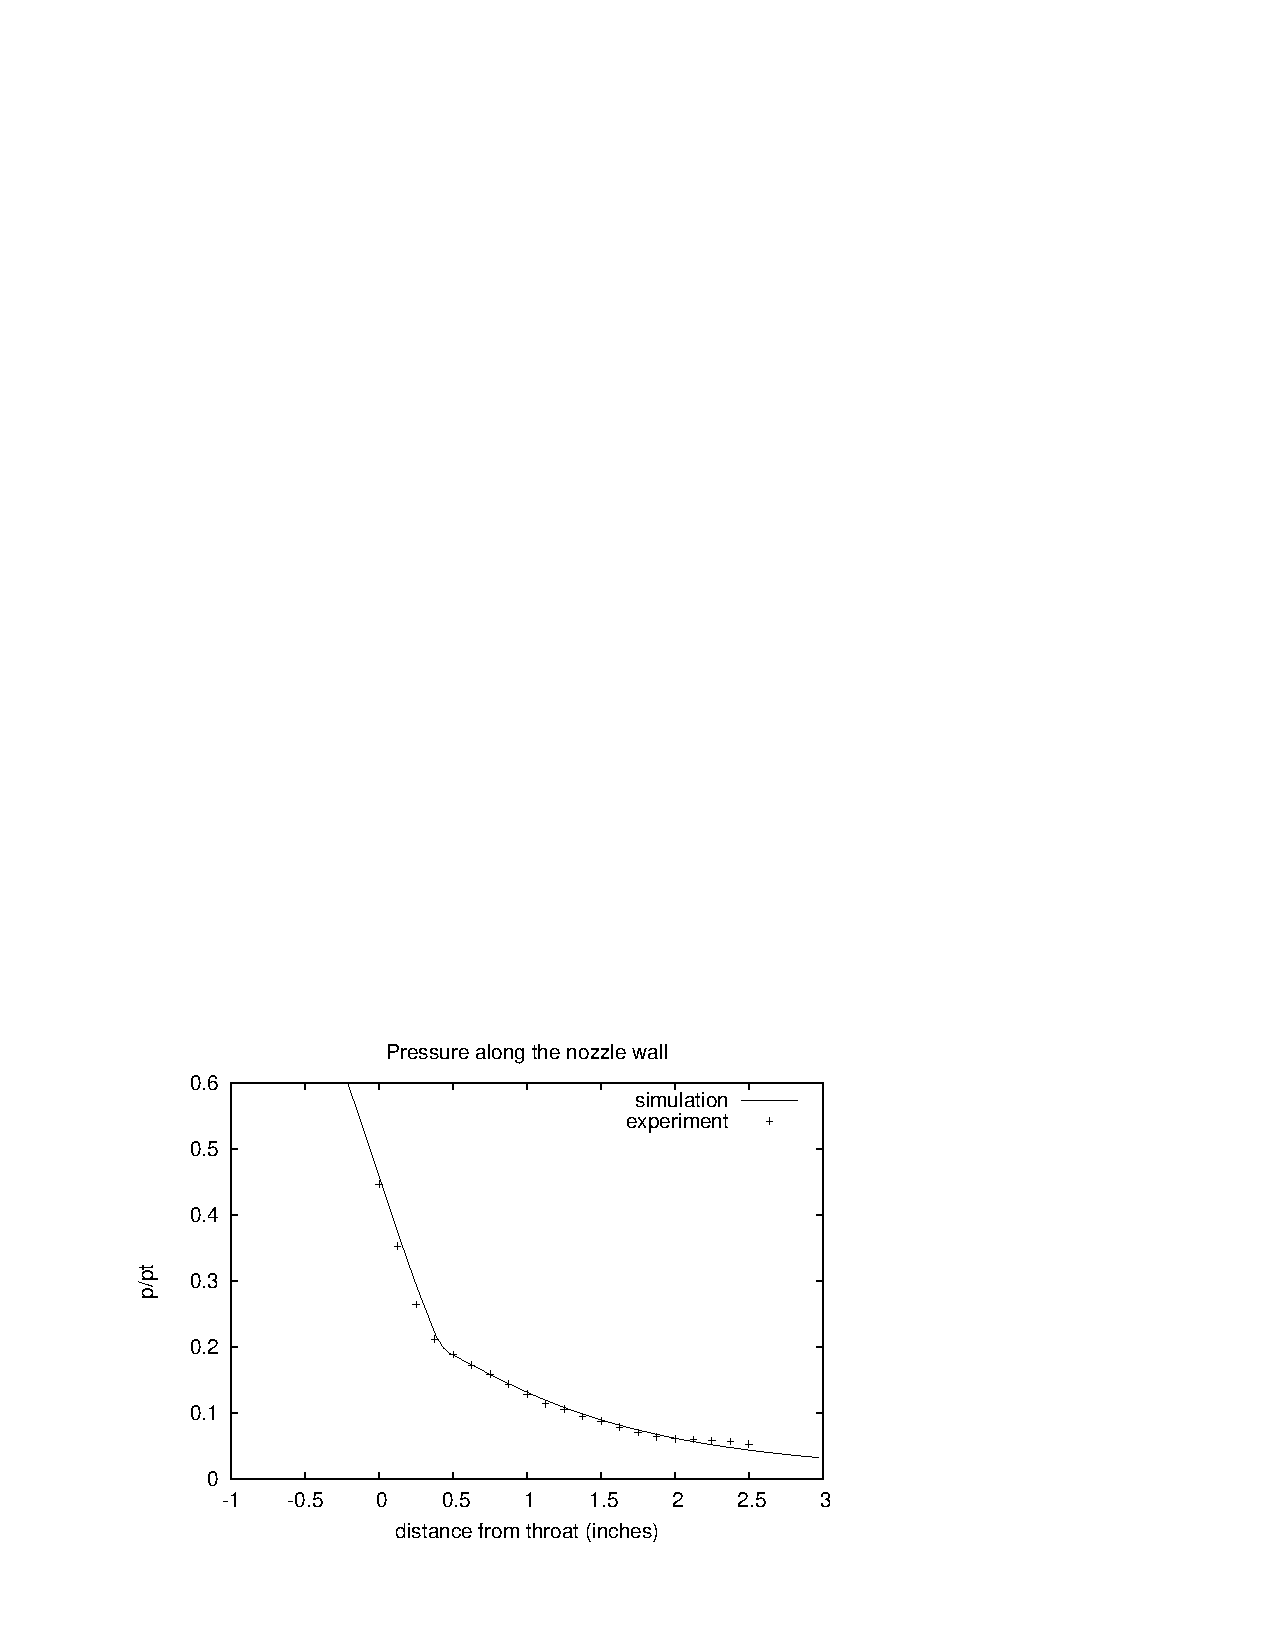
\includegraphics[width=0.5\textwidth]{../2D/back-nozzle/back_profile_supersonic.pdf}
\end{tabular}
\end{center}
\caption{Normalised pressure distribution along the nozzle wall:
         (a) full length of flow domain; 
	 (b) just the supersonic part of the nozzle.}
\label{back-profile-fig}
\end{figure}

\newpage
\subsection{Input script (.py)}
\topbar
\lstinputlisting[language={}]{../2D/back-nozzle/back.py}
\bottombar


\subsection{Shell scripts}
\label{back-sh-files}
\topbar
\lstinputlisting[language={}]{../2D/back-nozzle/back_run.sh}
\bottombar

\noindent
\topbar
\lstinputlisting[language={}]{../2D/back-nozzle/back_profile.sh}
\bottombar

\noindent
\topbar
\lstinputlisting[language={}]{../2D/back-nozzle/back_history.sh}\index{history location!extracting the data}
\bottombar

\newpage
\subsection{Notes}
\begin{itemize}
\item The simulation reaches a final time of 4\,ms in 5410 steps and,
      on an AMD Phenom II X4 840 system, this takes 128 seconds run time.
\item The pressure is normalised with respect to the stagnation pressure
      using the following AWK script.\\
      \topbarshort
      \lstinputlisting[language={}]{../2D/back-nozzle/normalize.awk}
      \bottombarshort\\
\item The history data for all of the history cells in a particular block are
      written to the one file.
      A particular cell can be extracted as shown by the following AWK script.\\
      \topbarshort
      \lstinputlisting[language={}]{../2D/back-nozzle/extract-history.awk}
      \bottombarshort\\
\end{itemize}

\cleardoublepage
% sawada-sphere.tex

\newpage
\section{Flow of equilibrium air over a sphere}
\index{gas model!look-up table!example of use}
%
This example is a good starting-point for the modelling of 
hypersonic flow over blunt bodies. 
It shows the use of arcs and the use of a look-up table 
as the equation of state for a gas in chemical equilibrium but
it remains geometrically simple by using a single-block grid.
Also, the .py file makes use of the Python language to parameterize
the simulation's specification.


\begin{figure}[htbp]
\begin{center}
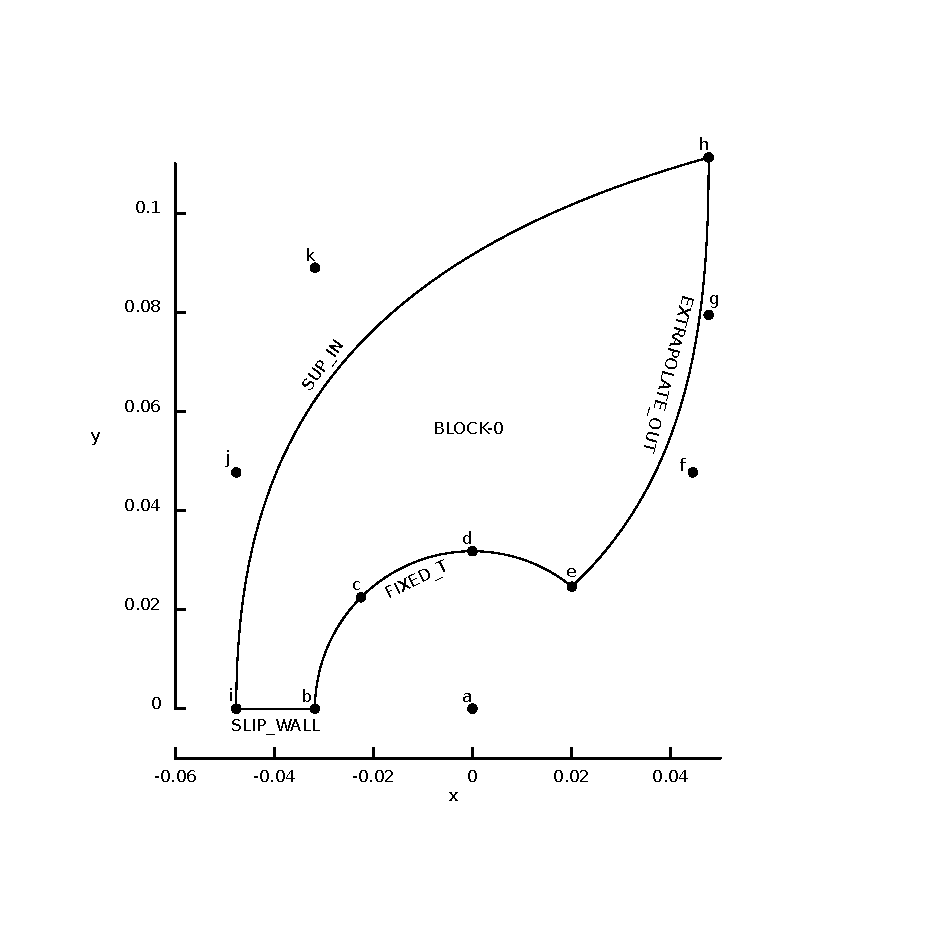
\includegraphics[width=10cm,viewport=41 69 346 388,clip=true]{../2D/sawada_sphere/ss3-layout.pdf}
\end{center}
\caption{Schematic diagram of the geometry for a sphere 
         wrapped by a single-block grid.}
\label{sawada-geometry-fig}
\end{figure}

\begin{figure}[htbp]
\begin{center}
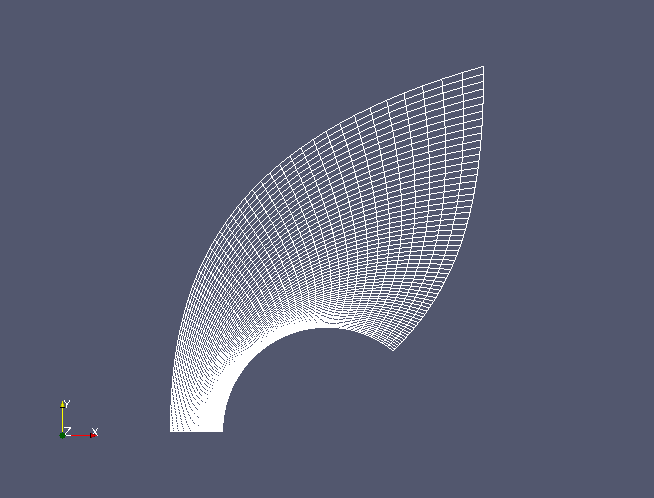
\includegraphics[width=12cm]{../2D/sawada_sphere/ss3-mesh.png}
\end{center}
\caption{Mesh for flow over a sphere.}
\label{sawada-mesh-fig}
\end{figure}

\medskip
The free-stream condition ($p_{\infty} = 20$\,kPa, $T_{\infty} = 296$\,K,
$u_{\infty} = 4.68$\,km/s) corresponds to Case 3 in 
Ref.~\cite{sawada_dendou_2001a} with $M_{\infty} = 13.6$.
According to Sawada \& Dendou  \cite{sawada_dendou_2001a}, the air is close
to being in chemical equilibrium and there is a very thin boundary layer. 
The results show that the inviscid simulation does indeed capture some 
of the high-temperature chemistry influence.
Ideal stagnation temperature would be 11204\,K whereas the simulated
temperature along the stagnation line rises to only 6081\,K. 
Secondly, the stand-off distance for an ideal gas is expected to be
approximately 4.63\,mm.
In Fig.~\ref{sawada-T-field-fig} the simulated shock 
stand-off distance is 2.66\,mm near the stagnation point.
This is within 3\% of the experimental value obtained by D.\,Reda in
Sandia's Ballistics Range (see \cite{sawada_dendou_2001a}).

\begin{figure}[htbp]
\begin{center}
\mbox{
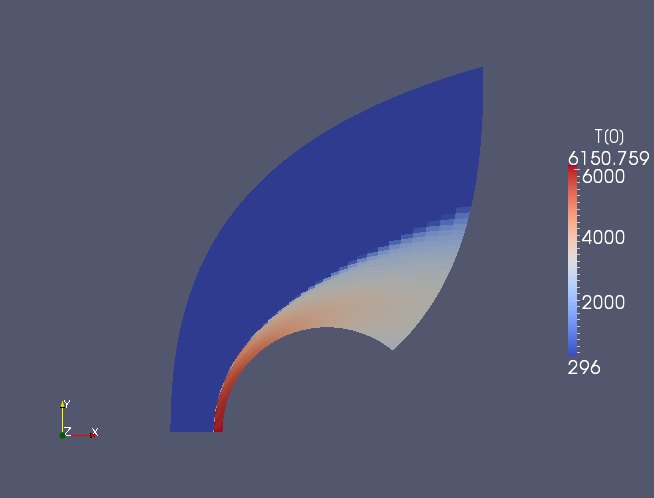
\includegraphics[width=0.5\textwidth]{../2D/sawada_sphere/ss3-T-field.png}
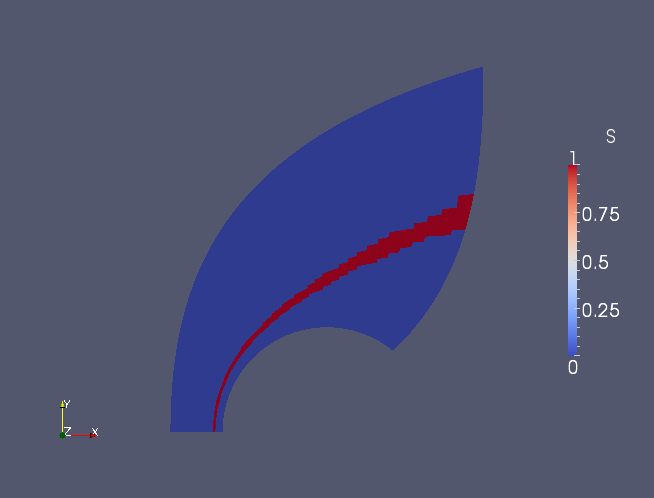
\includegraphics[width=0.5\textwidth]{../2D/sawada_sphere/ss3-S-field.png}
}
\end{center}
\caption{Temperature field and shock-detector (S) for equilibrium-air flow over a sphere.}
\label{sawada-T-field-fig}
\end{figure}


\subsection{Input script (.py)}
\topbar
\lstinputlisting[language={}]{../2D/sawada_sphere/ss3.py}
\bottombar

\newpage
\subsection{Shell scripts}
\label{sawada-sh-files}
The \texttt{ss3\_setup\_lut.sh} script assumes a ``standard'' location
for the \texttt{e3bin} directories in order to find the files for the look-up-table gas model.
The first form of the look-up-table has been generated as a regular array 
of sample points over ranges of density and temperature.
When reformatting the table to have a regular array of data points over
density and internal-energy, there is an option \texttt{--extrapolate} to instruct
the program to extrapolate when necessary.
When this option is not given, the final table covers smaller ranges
of density and internal-energy that fall completely within the original sampled data.\\
\topbar
\lstinputlisting[language={}]{../2D/sawada_sphere/ss3_setup_lut.sh}
\bottombar

\noindent
\topbar
\lstinputlisting[language={}]{../2D/sawada_sphere/ss3_run_py.sh}
\bottombar

\noindent
\topbar
\lstinputlisting[language={}]{../2D/sawada_sphere/ss3_post.sh}
\bottombar

\newpage
\subsection{Notes}
\begin{itemize}
\item Going back a couple of years, the mbcns2 simulation finished at 
      a final time of 67.95\,$\mu$s in 4548 steps and,
      on a Pentium-M 1.73\,Ghz system, this took 5\,min, 6\,s of CPU time.
      Eilmer3 is a bit slower, requiring 8\,min, 38\,s of CPU time
      on a Pentium E2140 (1.6\,GHz) for 4556 steps.
\item Awk script for extracting the shock location from the stagnation-line
      flow data.
      \lstinputlisting[language={}]{../2D/sawada_sphere/locate_shock.awk}
\end{itemize}

\cleardoublepage
% classic-shock-tube.tex

\section{Classic shock tube problem}
%
This example is a variation of the ``Sod'' shock tube problem that is a classic
test case for transient flow simulation codes.
It models a 1 metre long tube with hot, high-pressure helium in the left half (driver) and
low-pressure air in the right half (driven) part of the tube.
The conditions are such that high-temperature thermochemical effects are significant
in the shock-compressed air that is driven to the right from $t=0$.

\begin{figure}[htbp]
\begin{center}
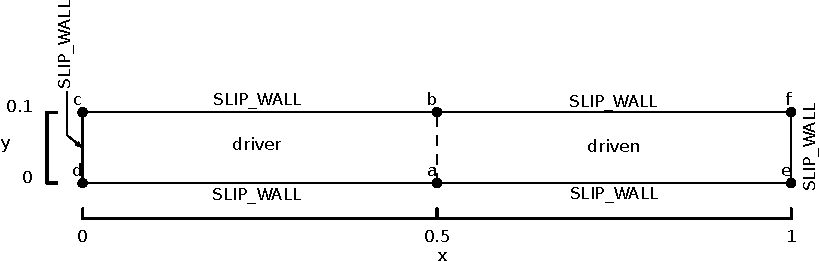
\includegraphics[width=0.9\textwidth]{../2D/classic-shock-tube/cst-edited.pdf}
\end{center}
\caption{Flow region, as modelled, for the classic shock tube.}
\label{cst-model-fig}
\end{figure}

Run the case with the following commands:\\
%
\topbar\\
\texttt{\$ cd $\sim$/cfcfd3/examples/eilmer3/2D/classic-shock-tube/}\\
\texttt{\$ ./prep\_simulation.sh}\\
\texttt{\$ ./run\_simulation.sh}\\
\texttt{\$ ./post\_simulation.sh}\\
\bottombar\\
%

The simulation is run for 100\,$\mu$s and the data is extracted for plotting against
the expected solution, as shown in Figure\,\ref{cst-profiles-fig}.
This reference solution is obtained using finite-wave and shock analysis assuming chemical equilibrium 
in the driven air.
The details of the calculation are found in Python script in Section\,\ref{finite-wave-sec}.

\begin{figure}[htbp]
\begin{tabular}{cc}
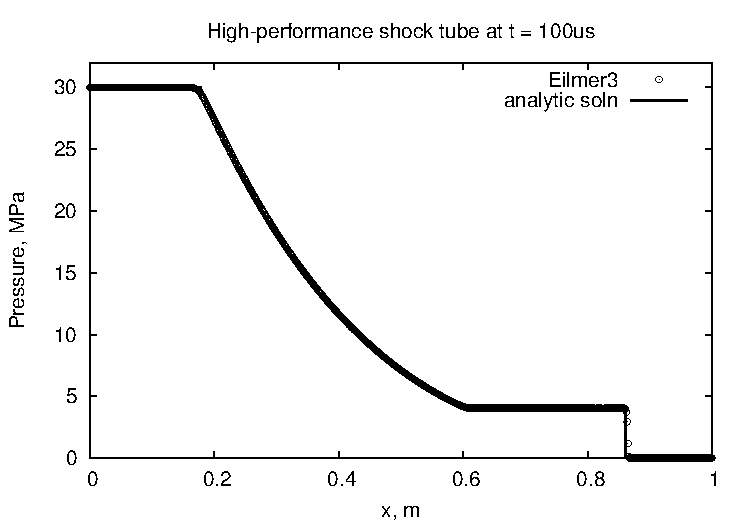
\includegraphics[width=0.5\textwidth]{../2D/classic-shock-tube/cst-p.pdf} &
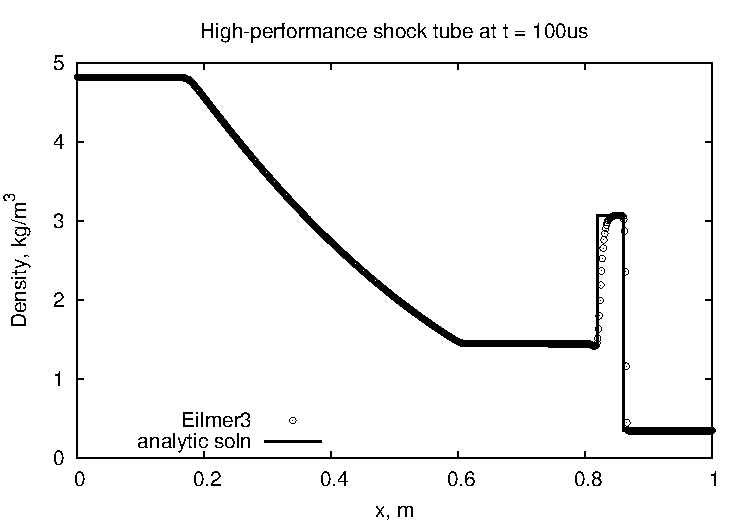
\includegraphics[width=0.5\textwidth]{../2D/classic-shock-tube/cst-rho.pdf}\\
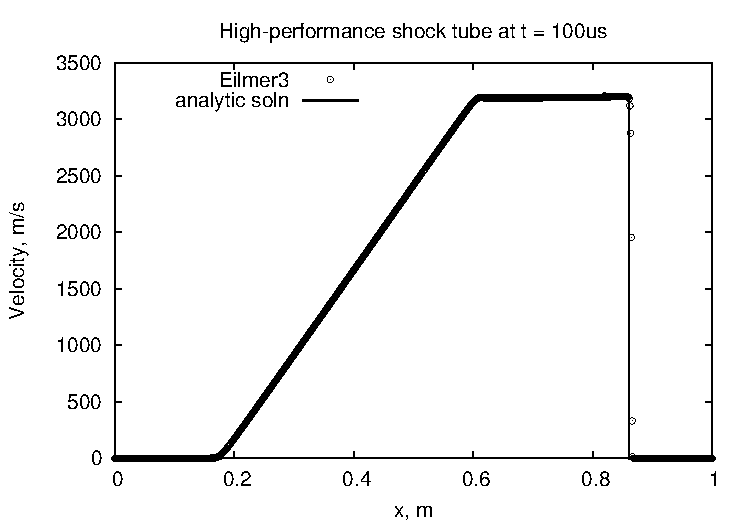
\includegraphics[width=0.5\textwidth]{../2D/classic-shock-tube/cst-u.pdf} &
\includegraphics[width=0.5\textwidth]{../2D/classic-shock-tube/cst-T.pdf}
\end{tabular}
\caption{Flow properties along the duct for the Sod shock tube problem for nni=400.}
\label{cst-profiles-fig}
\end{figure}

Convergence of the estimated shock speed (determined by locating the pressure jump with
the \texttt{locate\_shock.py} postprocessing script) is shown in Figure\,\ref{cst-convergence-fig}.
This custom postprocessing script also computes an average of the expended driver gas speed.

\begin{figure}[htbp]
\begin{center}
\includegraphics[width=0.6\textwidth]{../2D/classic-shock-tube/cst-errors.pdf}
\end{center}
\caption{Convergence of estimated shock speed and gas speed.}
\label{cst-convergence-fig}
\end{figure}

\newpage
\subsection{Input script (.py)}
\label{cst-py-file}
\index{gas model!look-up table!combined with composite-gas}
%
In the problem setup, below, note the combination of the look-up gas model with the composite gas model.
The helium driver gas is the only species in the composite gas and the look-up table gas models
all of the chemically-reacting species within the air test gas.
The look-up table gas ends up being prepended to the list of species for the simulation.

\noindent
\topbar
\lstinputlisting[language={}]{../2D/classic-shock-tube/cst.py}
\bottombar

\newpage
\subsection{Shell scripts}
\label{cst-sh-files}
\topbar
\lstinputlisting[language={}]{../2D/classic-shock-tube/prep_simulation.sh}
\bottombar

\noindent
\topbar
\lstinputlisting[language={}]{../2D/classic-shock-tube/run_simulation.sh}
\bottombar

\noindent
\topbar
\lstinputlisting[language={}]{../2D/classic-shock-tube/post_simulation.sh}
\bottombar

\noindent
\topbar
\lstinputlisting[language={}]{../2D/classic-shock-tube/plot_errors.sh}
\bottombar

\newpage
\subsection{Solution using finite wave and shock analysis}
\label{finite-wave-sec}
%
The NASA CEA program can be used by a library module to provide convenient estimates 
of the thermochemical state of gas mixtures at equilibrium.
The following script shows how to use that library to compute the flow for the classic
shock tube where the temperatures in the driven air test gas are large enough to 
allow significant thermochemical effects.
Beyond gas state estimation, the library provides analysis functions for simple 
flow processes such as shock and finite, isentropic waves.

\noindent
\topbar
\lstinputlisting[language={}]{../2D/classic-shock-tube/classic_shock_tube.py}
\bottombar

\newpage
\subsection{Extracting shock location and getting average gas speed}
%
\index{postprocessing!customized!shock location}
The following script is and example of how to pick up a full block of data
with the post-processing library functions and then look within that flow data
for particular features.

\noindent
\topbar
\lstinputlisting[language={}]{../2D/classic-shock-tube/locate_shock.py}
\bottombar

\subsection{Notes}
\begin{itemize}
\item The simulation with \texttt{nni = 400} takes about 13\,seconds on a recent (2011) machine 
  with an AMD Phenom 9650 quad-core processor.
\end{itemize}

\cleardoublepage
% sphere-heat-transfer.tex

\newpage
\section{Heat transfer to a sphere in equilibrium air}
\label{sphere-heat-transfer-sec}
\index{gas model!look-up table!example of use}
%
This example continues the modelling of hypersonic flow over blunt bodies 
and looks at the heat transfer to a spherical probe \cite{rose_stark_58} in high temperature equilibrium air. 
It takes use of the Python language further by automating the process of running 
a simulation, adjusting the grid and then running a subsequent simulation on the
the adjusted grid.
The specific input file for each stage of the overall simulation is constructed from a template
in which a few parameters are left unspecified.
Most of the effort has gone into the coordinating script which has functions
for running stages of the simulation as subprocesses and also has functions
which fit a Bezier curve to the shock located in the flow field.

\begin{figure}[htbp]
\begin{center}
\includegraphics[width=10cm,viewport=23 70 296 351,clip=true]{../2D/sphere-heat-transfer/sphere0-layout.pdf}
\end{center}
\caption{Schematic diagram of the geometry for a sphere wrapped by a SuperBlock2D grid.}
\label{sphere-heat-transfer-geometry-fig}
\end{figure}

\medskip
The original experiments used a probe with a spherical nose, located in a small shock tube.
The free-stream flow was initiated with the arrival of a strong shock and the useful test period 
in the experiments was terminated with the arrival of driver gas.
From Figure\,12 in Rose and Detra's paper \cite{rose_stark_58}, we choose the point corresponding to
$p_1 = 1$\,cm Hg (1.33\,kPa) and $M_s$=8 which has a stagnation-point heat transfer of $30\pm2.0\,{\rm MW/m}^2$.
To keep the grid resolution requirements small,
we will start with an initial test gas pressure $p_1 = 6.7$\,Pa much lower 
than that used in the original experiments.  
Assuming that the chemistry doesn't change too much with the change in pressure, we can scale the stagnation-point
heat transfer as $\dot{q}_{s-sim} = \left( \frac{p_{1-sim}}{p_{1-expt}} \right)^{0.5} \dot{q}_{s-expt}$ 
to get an expected value of $2.212\pm0.14\,{\rm MW/m}^2$ for our low-pressure simulation.

\medskip
For a $M_s = 8$ incident shock in air at 296\,K, the post-shock, free-stream conditions
are $p_{\infty} = 535.6$\,kPa, $T_{\infty} = 2573.5$\,K, and $u_{\infty} = 2436.5$\,m/s.
This assumes fully-equilibrium chemistry for the gas.
The snap-shots of results for the staged simulation are shown in Figures \ref{sphere-heat-transfer-stage-0-fig} through
\ref{sphere-heat-transfer-stage-4-fig} which show the temperature field at the end of each stage
and the mesh used for that stage. 

\begin{figure}[htbp]
\begin{center}
\mbox{
\includegraphics[width=0.4\textwidth]{../2D/sphere-heat-transfer/sphere0-T-field.png}
\includegraphics[width=0.4\textwidth]{../2D/sphere-heat-transfer/sphere0-mesh.png}
}
\end{center}
\caption{Temperature field and mesh for stage 0.  
  The control points for the Bezier curve have been set so as to accommodate 
  a shock in ideal (nonreacting) air and the clustering is fairly strong so that
  the boundary layer on the sphere surface may be resolved.
  The wall-clock time required to run this simulation 10 body lengths (27$\mu$s) is 23 seconds 
  on 4 processors of \texttt{geyser}.
  10103 time steps were made and the size of the time step at the end of the simulation is 2.479\,ns.
  At the end of the simulation, the estimated value of stagnation-point heat transfer is
  $\dot{q}_s=2.156\,{\rm MW/m}^2$ and the cell Reynolds number at the stagnation point is
  ${\rm Re}_{wall} = {{\rho_{wall} a_{wall} \Delta x} \over {\mu_{wall}}} = 3.85$.
  Here $\Delta x$ is the width of the cell out from the wall.}
\label{sphere-heat-transfer-stage-0-fig}
\end{figure}

\begin{figure}[htbp]
\begin{center}
\mbox{
\includegraphics[width=0.4\textwidth]{../2D/sphere-heat-transfer/sphere1-T-field.png}
\includegraphics[width=0.4\textwidth]{../2D/sphere-heat-transfer/sphere1-mesh.png}
}
\end{center}
\caption{Temperature field and mesh for stage 1.
  The Bezier points have been adapted to the shock from stage 0 but the number of cells
  in each direction remains at 20$\times$20, as for stage 0.
  With the finer cells, the size of the time step decreased and this stage required 55 seconds of wall-clock time
  to extend the simulation a further 10 body lengths in 23125 time steps.
  $\dot{q}_s=2.260\,{\rm MW/m}^2$ and ${\rm Re}_{wall} =2.94$}
\label{sphere-heat-transfer-stage-1-fig}
\end{figure}

\begin{figure}[htbp]
\begin{center}
\mbox{
\includegraphics[width=0.4\textwidth]{../2D/sphere-heat-transfer/sphere2-T-field.png}
\includegraphics[width=0.4\textwidth]{../2D/sphere-heat-transfer/sphere2-mesh.png}
}
\end{center}
\caption{Temperature field and mesh for stage 2.
  The Bezier points have not been adapted further for this stage but the number of cells
  has been increased to 30$\times$30.
  The size of the time step decreased further and this stage required 130 seconds of wall-clock time
  to extend the simulation only 5 body lengths (13.5\,$\mu$s) in 24293 time steps.
  $\dot{q}_s=2.257\,{\rm MW/m}^2$ and ${\rm Re}_{wall} =2.39$}
\label{sphere-heat-transfer-stage-2-fig}
\end{figure}

\begin{figure}[htbp]
\begin{center}
\mbox{
\includegraphics[width=0.4\textwidth]{../2D/sphere-heat-transfer/sphere3-T-field.png}
\includegraphics[width=0.4\textwidth]{../2D/sphere-heat-transfer/sphere3-mesh.png}
}
\end{center}
\caption{Temperature field and mesh for stage 3.
  The Bezier points have been adapted to the shock from stage 2 
  and the cells have been increased to 40$\times$40.
  The size of the time step is now 0.319\,ns and this stage required 469 seconds of wall-clock time
  to extend the simulation only 5 body lengths (13.5\,$\mu$s) in 42660 time steps.
  $\dot{q}_s = 2.260\,{\rm MW/m}^2$ and ${\rm Re}_{wall} =1.99$}.
\label{sphere-heat-transfer-stage-3-fig}
\end{figure}

\begin{figure}[htbp]
\begin{center}
\mbox{
\includegraphics[width=0.4\textwidth]{../2D/sphere-heat-transfer/sphere4-T-field.png}
\includegraphics[width=0.4\textwidth]{../2D/sphere-heat-transfer/sphere4-mesh.png}
}
\end{center}
\caption{Temperature field and mesh for stage 4.
  The Bezier points have not been further adapted but the number of cells has been
  increased to 80$\times$80 to test the sensitivity of the heat transfer estimate.
  The size of the time step is now 0.086\,ns and this stage required 8950 seconds of wall-clock time
  to extend the simulation a further 5 body lengths (13.5\,$\mu$s) in 157420 time steps.
  $\dot{q}_s =2 .217\,{\rm MW/m}^2$ and ${\rm Re}_{wall} = 1.25$}.
\label{sphere-heat-transfer-stage-4-fig}
\end{figure}

Figure \ref{sphere-norm-heat-transfer-fig} shows the distribution of heat transfer around the nose
compared with the experimental data reported Kemp, Rose and Detra \cite{kemp_etal_1959}.
In the simulation data, there are small distrubances at the corners of blocks 
(at approximately 20 degrees and then again approaching 90 degrees) but they are quite small.

\begin{figure}[htbp]
\begin{center}
\includegraphics[width=12cm]{../2D/sphere-heat-transfer/sphere_norm_heat_transfer.pdf}
\end{center}
\caption{Temperature around the sphere for stage 4.  
   The experimental data is from Kemp, Rose and Detra \cite{kemp_etal_1959}.}.
\label{sphere-norm-heat-transfer-fig}
\end{figure}

\clearpage

\subsection{Template input script (.py)}\index{ExistingSolution!example of use}\index{univariate function!RobertsClusterFunction!example of use}
\topbar
\lstinputlisting[language={}]{../2D/sphere-heat-transfer/sphere.input.template}
\bottombar

\subsection{Coordinating script (.py)}
\topbar
\lstinputlisting[language={}]{../2D/sphere-heat-transfer/run_adaptive_simulation.py}
\bottombar

\newpage
\subsection{Shell script for postprocessing}
\topbar
\lstinputlisting[language={}]{../2D/sphere-heat-transfer/plot_heat_transfer.sh}
\bottombar

\newpage
\subsection{Notes}
\begin{itemize}
\item The look-up table for the equilibrium air equation of state is set up 
   as for the Sawada sphere example.
\end{itemize}

\cleardoublepage
% n90.tex

\section{Dissociating N$_2$ flow over a 2D cylinder}
\label{sec:n90}
\index{chemical reaction!example of use}
\index{finite-rate chemistry|see {chemical reaction}}
\index{gas model!thermally perfect!example of use}
%
High speed flow of nitrogen over a 2D cylinder is a signature experiment for shock tunnel
and expansion tube facilities.
This example shows the construction of a simple flow domain around a circular cylinder
and the set up of a finite-rate reacting model for dissociating nitrogen.
The data for comparison has come from our colleagues ar DLR-G\"{o}ttingen.

\begin{figure}[htbp]
\begin{center}
\includegraphics[width=12cm,viewport=76 80 391 439,clip=true]{../2D/n90/n90-schematic.pdf}
\end{center}
\caption{Schematic diagram of the geometry for the bluff body.}
\label{n90-geometry-fig}
\end{figure}

\begin{figure}[htbp]
\begin{center}
\includegraphics[width=\textwidth]{../2D/n90/n90-pressure-mesh.png}
\end{center}
\caption{Mesh, coloured by pressure, for the n90 bluff body exercise.}
\label{n90-mesh-fig}
\end{figure}

\begin{figure}[htbp]
\begin{center}
\includegraphics[width=12cm, viewport=67 53 403 291]{../2D/n90/n90_compare_T_stag_line.pdf}
\end{center}
\caption{Temperature data along the stagnation streamline.}
\label{n90-stag-line-temp-fig}
\end{figure}

\begin{figure}[htbp]
\begin{center}
\mbox{
\includegraphics[width=0.5\textwidth]{../2D/n90/n90-temperature.png}
\includegraphics[width=0.5\textwidth]{../2D/n90/n90-massf1.png}
}
\end{center}
\caption{Temperature and mass fraction of nitrogen atoms for the n90 bluff body exercise.}
\label{n90-temperature-massf-fig}
\end{figure}

\newpage

\subsection{Input script (.py)}
\topbar
\lstinputlisting[language={}]{../2D/n90/n90.py}
\bottombar

\subsection{Reaction scheme file (.lua)}\index{chemical reaction!reaction scheme file!dissociating nitrogen}
\topbar
\lstinputlisting[language={}]{../2D/n90/nitrogen-2sp-2r.lua}
\bottombar

\subsection{Shell scripts}
\label{n90-sh-files}
\topbar
\lstinputlisting[language={}]{../2D/n90/prepare_simulation.sh}
\bottombar

\noindent
\topbar
\lstinputlisting[language={}]{../2D/n90/run_simulation.sh}
\bottombar

\noindent
\topbar
\lstinputlisting[language={}]{../2D/n90/post_simulation.sh}
\bottombar

\noindent
\topbar
\lstinputlisting[language={}]{../2D/n90/plot_comparison.gnu}
\bottombar

\subsection{Notes}
\begin{itemize}
\item For Eilmer3, this simulation required 9\,min, 21\,sec on a single core of 
  a Pentium 1.6\,GHz processor to reach a final time of 100$\mu$s in 3406 steps.
\end{itemize}

\cleardoublepage
% lehr-sphere.tex

\newpage
\section{Flow of detonable mixture over a sphere}
\index{chemical reaction!example of use}
\index{gas model!thermally perfect!example of use}
%
Interesting things can happen when the chemical-reaction time scales
are of the same order as the flow time scales. 
This example simulates the flow of a stoichiometric mixture of hydrogen and air over
the spherical nose of a projectile as used by Lehr in some ballistic range experiments
\cite{lehr_1972}.
For a range of Mach numbers, the combustion of the hydrogen is unsteady so it provides
an interesting test of the interaction of the gas dynamics and chemical kinetics modules
of the code.
Figure\,\ref{lehr-expt-M479-fig} shows the periodic structure caused by the unsteady combustion 
of the gas mixture over the projectile.

\begin{figure}[htbp]
\begin{center}
\includegraphics[width=10cm]{../2D/lehr-479/lehr-M4p79-scanned-image-from-wilson-thesis.jpg}
\end{center}
\caption{Shadowgraph of the unsteady flow of reacting hydrogen and air over a ballistic-range
  projectile at a Mach number of 4.79.  This particular image has been scanned from Greg Wilson's
  PhD thesis \cite{wilson_1991}.}
\label{lehr-expt-M479-fig}
\end{figure}

\medskip
The free-stream condition is $p_{\infty} = 320$\,mm\,Hg, $T_{\infty} = 292$\,K,
$u_{\infty} = 1.931$\,km/s, corresponding to a Mach number of 4.79 in a stoichiometric mixture
of hydrogen and air (nitrogen + oxygen only).
The small calculation to get actual mass fraction of each species is done as part of the user input script.
For this flight condition, Lehr observed a frequency of oscillation of 0.72\,MHz. 

\medskip
Because this example is just a demonstration of the code capability and not a validation
and because the case takes a day or two to run on 4 processors of geyser,
we settle for the use of a reduced chemical reaction scheme in which nitrogen is assumed to be
a non-reacting diluent gas.
This is done near the top of the the reaction scheme file \ref{lehr-reaction-file} 
by selecting \texttt{INERT\_N2} as the model.

\begin{figure}[htbp]
\begin{center}
\includegraphics[width=10cm,viewport=43 73 288 344,clip=true]{../2D/lehr-479/lehr-layout.pdf}
\end{center}
\caption{Schematic diagram of the geometry for a sphere wrapped by a SuperBlock2D grid.
   Although $2 \times 2$ blocks are shown here, we are typically impatient and 
   use $4 \times 6$ blocks as shown in the input scripts.}
\label{lehr-geometry-fig}
\end{figure}

\medskip
If we start very reasonably, with a low-resolution grid and do the calculation fairly in short order,
we get something like the left image in Figure\,\ref{lehr-T-field-fig}.
The solution is all very steady, well behaved, and quite wrong.
The reaction front has merged into the shock and the whole shock layer has inflated to a stand-off distance
significantly larger than that observed in the experiment.
Just increasing the grid resolution (by a factor of 10 in each direction) provided a solution as shown in the right
side of Figure\,\ref{lehr-T-field-fig}.
Here, the reaction front is clearly separated from the incident shock, and it is not smooth.
Although it is not clear from this particular image, there is a periodic large scale disturbance 
to the reaction front, and a slightly smaller disturbance to the shock front.

\begin{figure}[htbp]
\begin{center}
\mbox{
\includegraphics[width=0.45\textwidth]{../2D/lehr-479/lehr-479-T-field-t0019-20x30.png}
\includegraphics[width=0.45\textwidth]{../2D/lehr-479/lehr-479-T-field-t0019-200x300.png}
}
\end{center}
\caption{Temperature field at t=190\,$\mu$s for 20$\times$30 cells (left) and 200$\times$300 cells (right).}
\label{lehr-T-field-fig}
\end{figure}

\medskip
Figure \ref{lehr-density-field-fig} shows the density field for a few frames 
of the second-stage simulation (\texttt{lehr1.py}) over roughly one period of the large-scale oscillation.
Although the periodic nature of the flow is captured, the detailed behaviour of the reaction front 
is quite sensitive to grid resolution and the details of the reaction mechanism.
The frequency of the large scale oscillation in this simulation is a long way short of the 0.72\,MHz 
observed by Lehr.
It is left as an exercise for the reader to try the more complete reaction schemes to see if the frequency 
of the flow oscillation can be better approximated.

\begin{figure}[htbp]
\begin{center}
\mbox{
\includegraphics[width=0.25\textwidth]{../2D/lehr-479/lehr1-density-field-200x300-frame-11.png}
\includegraphics[width=0.25\textwidth]{../2D/lehr-479/lehr1-density-field-200x300-frame-14.png}
\includegraphics[width=0.25\textwidth]{../2D/lehr-479/lehr1-density-field-200x300-frame-17.png}
\includegraphics[width=0.25\textwidth]{../2D/lehr-479/lehr1-density-field-200x300-frame-20.png}
}
\end{center}
\caption{Density field at t=11, 14, 17, 20\,$\mu$s in the \texttt{lehr1} second-stage simulation.}
\label{lehr-density-field-fig}
\end{figure}


\subsection{Input script (.py)}
\topbar
\lstinputlisting[language={}]{../2D/lehr-479/lehr.py}
\bottombar

\medskip\noindent
The second input script continues the simulation on a grid where the inflow boundary 
has been moved in toward the bow shock.
This makes better use of the computational resources as more cells are now within the shock layer.
\index{ExistingSolution!example of use}

\noindent
\topbar
\lstinputlisting[language={}]{../2D/lehr-479/lehr1.py}
\bottombar

\newpage
\subsection{Reaction scheme file (.lua)}\index{chemical reaction!reaction scheme file!H2-air combustion}
\label{lehr-reaction-file}
\topbar
\lstinputlisting[language={}]{../2D/lehr-479/Evans_Schexnayder.lua}
\bottombar

\medskip
\subsection{Notes}
\begin{itemize}
\item None
\end{itemize}

\cleardoublepage
% mnm-implosion-problem.tex

\section{MNM implosion problem}
\label{mnm-implosion-sec}
%
This example shows the use of the Python functions to set up
a very simple flow geometry with a reasonably complex initial flow state 
and then to test the symmetry of the computed flow solution.
This test was suggested by Dr. Michael Macrossan.
The flow field should be axisymmetric but it is computed on a square grid,
so any grid-aligned flux calculation problems should be highlighted.
Run the case with the following commands:\\
%
\topbar\\
\texttt{\$ cd $\sim$/cfcfd3/examples/eilmer3/2D/implosion/}\\
\texttt{\$ ./imp\_run.sh}\\
\bottombar\\
%
and, within a couple of minutes, you should end up with a number of files
with various solution data plotted.
Figure\,\ref{implosion-initial-density-fig} shows the initial density field
in a quiescent gas.
This field is approximately axisymmetric and is initialized by computing an estimate
for fraction of each cell inside the nominal radius of 1.0 and then weighting the
density value by that fraction.
The code for this calculation dominates the imput script in Section\,\ref{implosion-py-file}

\begin{figure}[htbp]
\begin{center}
\includegraphics[width=10cm]{../2D/implosion/density-t0000.png}
\end{center}
\caption{Initial density field for the implosion problem.}
\label{implosion-initial-density-fig}
\end{figure}

\medskip
Figure\,\ref{implosion-final-density-fig} shows the density field at the end of
time-stepping, when $t=0.296 ~ \frac{L}{a}$ where $a$ is the initial sound speed of the gas
and L is a nominal length scale.
At this time the shock has propagated into the origin, reflected and passed back out 
through the contact surface.
Symmetry of the solution is not perfect but it is pretty good.
Figure\,\ref{implosion-density-profiles-fig} shows the density profiles for a number of radial slices.


\begin{figure}[htbp]
\begin{center}
\includegraphics[width=10cm]{../2D/implosion/density-t9999.png}
\end{center}
\caption{Final density field for the implosion problem.}
\label{implosion-final-density-fig}
\end{figure}

\begin{figure}[htbp]
\begin{center}
\includegraphics[width=10cm,viewport=55 49 397 293,clip=true]{../2D/implosion/density-vs-radius.pdf}
\end{center}
\caption{Density profiles at the final time for the implosion problem.}
\label{implosion-density-profiles-fig}
\end{figure}

\medskip

\newpage

\subsection{Input script (.py)}\index{geometric element!PyFunctionSurface!example of use}
\index{gas model!change\_ideal\_gas\_attribute!example of use}
\label{implosion-py-file}
\topbar
\lstinputlisting[language={}]{../2D/implosion/imp.py}
\bottombar


\subsection{Shell scripts}
\label{implosion-sh-files}
\topbar
\lstinputlisting[language={}]{../2D/implosion/imp_run.sh}
\bottombar

\subsection{Notes}
\begin{itemize}
\item This example shows how to change an attribute of the ideal gas model,
  specifically, the ratio of specific heats.
  Look for the call to the function \texttt{change\_ideal\_gas\_attribute}
  in the input script. 
\item It also shows off the \texttt{--slice-along-line} option for 
  the postprocessor \texttt{e3post.py}.
\end{itemize}

\cleardoublepage
% periodic-shear-layer.tex

\section{Periodic Shear Layer}\index{boundary conditions!periodic!example of use}
\label{periodic-shear-layer-sec}
%
This example shows the use of the Python functions to set up
a simple shear flow with a linear variation of velocity through the finite-width shear layer.
There is also a variation of species mass fractions of helium and air between the counterflowing streams.
The basic flow is intended to be somewhat representative of the fuel-air mixing layers
encountered in shock-tunnel tests of scramjets, however, the model flow here
is made periodic in the $x$-direction by connecting the block faces as shown in
Fig.\,\ref{psl-layout-fig}. 

\begin{figure}[htbp]
\begin{center}
\includegraphics[width=10cm,viewport=94 63 353 396,clip=true]{../2D/periodic-shear-layer/psl-layout.pdf}
\end{center}
\caption{Computational domain for the periodic shear layer.}
\label{psl-layout-fig}
\end{figure}

\medskip
Figure\,\ref{psl-mass-fraction-fig} shows the mass fraction of helium at several time instants through
the evolution of the shear layer.
The layer has started with almost parallel flow, with a relatively small velocity perturbation,
as defined in the function \texttt{initial\_gas()} in the input script (see Sec.\,\ref{psl-py-file}).

\clearpage

\begin{figure}[htbp]
\begin{center}
\mbox{
\includegraphics[width=0.25\textwidth]{../2D/periodic-shear-layer/psl-massf0-t00.png}
\includegraphics[width=0.25\textwidth]{../2D/periodic-shear-layer/psl-massf0-t05.png}
\includegraphics[width=0.25\textwidth]{../2D/periodic-shear-layer/psl-massf0-t10.png}
\includegraphics[width=0.25\textwidth]{../2D/periodic-shear-layer/psl-massf0-t15.png}
}
\end{center}
\caption{Mass fraction for helium across the periodic shear layer at times 0, 5.1\,ms, 10.2\,ms and 15\,ms.}
\label{psl-mass-fraction-fig}
\end{figure}

\medskip
Figure\,\ref{psl-vorticity-fig} shows the evolution of the vorticity field.
Vorticity is not part of the flow data files but can be computed within \texttt{Paraview}
by applying the following filters to the cell data:
\begin{itemize}
 \item \texttt{Gradient of Unstructured DataSet} selecting \texttt{vel.x} as the scalar and
    \texttt{du} as the result array name.
 \item \texttt{Gradient of Unstructured DataSet} selecting \texttt{vel.y} as the scalar and
    \texttt{dv} as the result array name.
 \item \texttt{Calculator} with \texttt{Cell Data} as the attribute mode, 
    \texttt{dv\_X - du\_Y} as the expression to compute, and \texttt{vorticity} as the result array name.
\end{itemize}
Note that there is a small defect in the vorticity values at the block boundaries.
This is an artifact of the \texttt{Paraview} calculation and not of the original simulation flow field.
 
\begin{figure}[htbp]
\begin{center}
\mbox{
\includegraphics[width=0.25\textwidth]{../2D/periodic-shear-layer/psl-vorticity-t00.png}
\includegraphics[width=0.25\textwidth]{../2D/periodic-shear-layer/psl-vorticity-t05.png}
\includegraphics[width=0.25\textwidth]{../2D/periodic-shear-layer/psl-vorticity-t10.png}
\includegraphics[width=0.25\textwidth]{../2D/periodic-shear-layer/psl-vorticity-t15.png}
}
\end{center}
\caption{Vorticity field for the periodic shear layer at times 0, 5.1\,ms, 10.2\,ms and 15\,ms.}
\label{psl-vorticity-fig}
\end{figure}

\newpage

\subsection{Input script (.py)}
\label{psl-py-file}
\index{FlowCondition!add\_to\_list parameter!example of use}
\topbar
\lstinputlisting[language={}]{../2D/periodic-shear-layer/psl.py}
\bottombar


\subsection{Shell scripts}
\label{psl-sh-files}
\topbar
\lstinputlisting[language={}]{../2D/periodic-shear-layer/prep_simulation.sh}
\bottombar \\
\topbar
\lstinputlisting[language={}]{../2D/periodic-shear-layer/run_simulation.sh}
\bottombar

\subsection{Notes}
\begin{itemize}
\item This simulation take 33707 steps and 28945\,seconds on 4 cores of geyser (AMD processors).
\end{itemize}

\cleardoublepage
% cone20-udf.tex

\section{Mach 1.5 flow over a 20$^o$ cone -- UDF boundaries}
\label{sec:cone20-udf}
%
This is a small (in both memory and run time) example 
that shows the implementation of user-defined boundary conditions.
It is otherwise equivalent to the case in Section\,\ref{cone20-simple-sec}.
Use the following commands:\\
%
\topbar\\
\texttt{\$ cd $\sim$/cfcfd2/examples/eilmer3/2D/cone20-udf}\\
\texttt{\$ ./cone20\_run.sh}\\
\bottombar\\
%
and, within a minute or so, you should end up with a number of files
with various solution data plotted.
The grid and initial solution are created and the time-evolution of the
flow field is computed for 5\,ms (with 1105 time steps being required).
The commands invoke the shell scripts displayed in 
subsection~\ref{cone20-udf-sh-files}.
%

\begin{figure}[htbp]
\begin{center}
\includegraphics[width=10cm, viewport=76 78 389 398]{../2D/cone20-udf/cone20_svg.pdf}
\end{center}
\caption{Schematic diagram of the geometry for a cone 
         with 20 degree half-angle and user-defined boundaries.}
\label{cone20-udf-geometry-fig}
\end{figure}

\medskip
The free-stream conditions ($p_{\infty} = 95.84$\,kPa, $T_{\infty} = 1103$\,K
and $u_{\infty} = 1000$\,m/s) are related to the shock-over-ramp test problem
in the original ICASE Report\,\cite{jacobs_91d} and are set to give a 
Mach number of 1.5.
From Chart 5 in Ref.\,\cite{ames_53}, the expected steady-state shock wave
angle is 49$^o$ and, from Chart 6, the pressure coefficent is
$$
\frac{p_{cone-surface} - p_{\infty}}{q_{\infty}} \approx 0.387
$$
and the dynamic pressure for the specified free stream is
$q_{\infty} = \frac{1}{2} \rho_{\infty} u_{\infty}^2 \approx 151.38$\,kPa.
Figure~\ref{cone20-udf-axial-force-fig} shows the pressure coefficient 
estimated as
$$
C_p = \frac{f_x - p_{\infty} A}{q_{\infty} A}
$$
from the simulated axial force, $f_x$, written into the simulation log file
and frontal area of the cone, $A$.

\begin{figure}[htbp]
\begin{center}
\includegraphics[width=0.8\textwidth, viewport=24 447 571 819]{../2D/cone20-udf/cone20_p.pdf}
\end{center}
\caption{Pressure data for flow over a cone with 20 degree half-angle.
         The shock profile is not yet straight and the pressure field
         near the cone surface is not conically symmetric, although it
	 would become more so if we continued the simulation.}
\label{cone20-udf-pressure-fig}
\end{figure}

\begin{figure}[htbp]
\begin{center}
\includegraphics[width=0.8\textwidth, viewport=24 447 571 819]{../2D/cone20-udf/cone20_S.pdf}
\end{center}
\caption{Shock-sensor data for flow over a cone with 20 degree half-angle.
         For the \texttt{adaptive} flux calculator, 
	 this sensor indicates the regions
	 of the flow where the more dissipative scheme should be used.}
\label{cone20-udf-shock-sensor-fig}
\end{figure}

\begin{figure}[htbp]
\begin{center}
\includegraphics[width=10cm, viewport=52 49 401 294]{../2D/cone20-udf/cone20_cp.pdf}
\end{center}
\caption{Evolution of the axial (drag) force
         for flow over a cone with 20 degree half-angle
	 for two mesh resolutions.}
\label{cone20-udf-axial-force-fig}
\end{figure}

\newpage

\subsection{Input script (.py)}\index{boundary conditions!UserDefinedBC!example of use}
\topbar
\lstinputlisting[language={}]{../2D/cone20-udf/cone20.py}
\bottombar

\newpage
\subsection{Boundary-condition files (.lua)}
\topbar
\lstinputlisting[language={}]{../2D/cone20-udf/udf-supersonic-in.lua}
\bottombar \\
\topbar
\lstinputlisting[language={}]{../2D/cone20-udf/udf-extrapolate-out.lua}
\bottombar \\
\topbar
\lstinputlisting[language={}]{../2D/cone20-udf/udf-slip-wall.lua}
\bottombar \\
\topbar
\lstinputlisting[language={}]{../2D/cone20-udf/udf-process.lua}
\bottombar

\subsection{Shell scripts}
\label{cone20-udf-sh-files}
\topbar
\lstinputlisting[language={}]{../2D/cone20-udf/cone20_run.sh}
\bottombar

\subsection{Notes}
\begin{itemize}
\item Run time is approximately 94 seconds for 1126 steps on a computer with 
      an Intel Dual Pentium E2160, 1.6\,GHz processor.  
      As would be expected, the calling of the user-defined (Lua) functions
      carries some cost, but not much.
\end{itemize}

\cleardoublepage
% vortex.tex
% see p18 of 2001/1 workbook 20-feb-2001
\section{A section of an ideal compressible-flow vortex}
\label{vortex-sec}
%
This flow example was used by Ian Johnston in his thesis 
and it comes with an analytic solution\,\cite{aftosmis_etal_1995a}.
With respect to \texttt{Eilmer3}, it illustrates the use of a specified flow profile as an input
and it shows the use of profile extraction, again.

The flow domain (Fig.\,\ref{vortex-geometry-fig}) includes only part of 
the first quadrant of an ideal vortex flow in inviscid air 
with $R=287$J/kg$\cdot$K, $\gamma$=1.4).
The NORTH and SOUTH boundaries are specified as reflecting walls
at radii $r_o$ and $r_i$, representing the outer and inner radii of the
vortex segment that is centred at node A.
The WEST boundary has the specified inflow as a function of radius
\begin{eqnarray}
   \rho(r) & = & \rho_i \left[
             1 + \frac{\gamma - 1}{2} M_i^2 
             \left\{ 1 - \left( \frac{r_i}{r} \right)^2 \right\}
             \right]^\frac{1}{\gamma - 1} ~~, \nonumber\\
   p(r) & = & p_i \left( \frac{\rho}{\rho_i} \right)^{\gamma} ~~, \nonumber \\
   u(r) & = & u_i \frac{r_i}{r} ~~, \nonumber
\end{eqnarray}
with $r_o = 1.384 r_i$ and the properties at the inner radius being
$M_i = 2.25$, $\rho_i = 1.0$\,kg/m$^3$ and $p_i = 100$\,kPa.

\begin{figure}[htbp]
\begin{center}
\includegraphics[width=9cm, viewport=71 74 392 392]{../2D/vortex/vtx-layout.pdf}
\end{center}
\caption{Schematic diagram of the first quadrant domain for 
         the compressible-flow vortex.}
\label{vortex-geometry-fig}
\end{figure}

Figure \ref{vortex-radial-fig} shows the radial distributions of flow properties 
and highlight some of the problems with 
the crude reflecting-wall boundary condition.
Other than at the boundaries, there is close agreement between the analytic
and numerical solutions.
The errors at the inner and outer radii stand out clearly because we
know that the trends of the flow property variations should continue
at these boundaries and not mirror what is just inside the flow domain.

\begin{figure}[htbp]
\begin{center}
\mbox{
\includegraphics[width=0.5\textwidth,viewport=66 60 408 292,clip=true]{../2D/vortex/radial_profile_p.pdf}
\includegraphics[width=0.5\textwidth,viewport=66 60 408 292,clip=true]{../2D/vortex/radial_profile_T.pdf}
}
\mbox{
\includegraphics[width=0.5\textwidth,viewport=66 60 408 292,clip=true]{../2D/vortex/radial_profile_u.pdf}
\includegraphics[width=0.5\textwidth]{../2D/vortex/vtx-speed-field.png}
}
\end{center}
\caption{Radial distributions of normalized pressure, temperature and velocity. 
  Also, the bottom right image shows the flow speed over the simulated domain}
\label{vortex-radial-fig}
\end{figure}


\newpage
\subsection{Input script (.py)}
\topbar
\lstinputlisting[language={}]{../2D/vortex/vtx.py}
\bottombar

\subsection{Boundary condition file (.lua)}
\topbar
\lstinputlisting[language={}]{../2D/vortex/udf-vortex-flow.lua}
\bottombar

\subsection{Shell scripts}
\label{vortex-sh-files}
\topbar
\lstinputlisting[language={}]{../2D/vortex/vtx_run.sh}
\bottombar

\noindent
\topbar
\lstinputlisting[language={}]{../2D/vortex/vtx_plot.sh}
\bottombar

\subsection{Notes}
\begin{itemize}
\item This simulation reaches a final time of 20\,ms in 2610 steps and,
      on an Intel Core 2 Duo CPU (E8400 @ 3.0\,Ghz) system, this takes 2\,min, 23\,s.
\item The plots were generated via the following scripts\\
      \topbarshort
      \lstinputlisting[language={}]{../2D/vortex/extract_radial.awk}
      \bottombarshort\\
      \topbarshort
      \lstinputlisting[language={}]{../2D/vortex/radial_profile.gnu}
      \bottombarshort\\
      \topbarshort
      \lstinputlisting[language={}]{../2D/vortex/make_profile.awk}
      \bottombarshort
\end{itemize}

\cleardoublepage
% mms-euler.tex

\section{Method of manufactured solutions -- Euler flow}
\index{source terms!user defined!example of use}\index{verification}
%
RJG's method of manufactured solutions as a code verification exercise.
This shows a sophisticated use of the user-defined source terms to
add the extra pieces required to model a known (manufactured) flow solution.

\begin{figure}[htbp]
\begin{center}
\mbox{
\includegraphics[width=0.5\textwidth]{../2D/mms_euler/mms-density.png}
\includegraphics[width=0.5\textwidth]{../2D/mms_euler/mms-pressure.png}
}
\end{center}
\caption{Density and pressure fields for the steady-state solution for the
  Method of Manufactured Solutions.}
\label{mms-euler-density-pressure-fig}
\end{figure}


\newpage

\subsection{Input script (.py)}\index{boundary conditions!UserDefinedBC!example of use}
\topbar
\lstinputlisting[language={}]{../2D/mms_euler/euler_manufactured.py}
\bottombar

\subsection{Boundary condition file (.lua)}
\topbar
\lstinputlisting[language={}]{../2D/mms_euler/udf-bc.lua}
\bottombar

\subsection{Source term file (.lua)}
%
The source terms were generated with the aid of the Maxima computer algebra system.
\topbar
\lstinputlisting[language={}]{../2D/mms_euler/udf-source.lua}
\bottombar

\subsection{Shell scripts}
\label{mms-euler-sh-files}
\topbar
\lstinputlisting[language={}]{../2D/mms_euler/prep_simulation.sh}
\bottombar

\noindent
\topbar
\lstinputlisting[language={}]{../2D/mms_euler/run_simulation.sh}
\bottombar

\noindent
The postprocessing script shows features of the post-processor that allow
one to compare one solution with another (in order to check convergence to steady state)
and also to report the norms of the differences between the computed solution and 
a reference solution described by a Python file.
\index{e3post.py!reference function}\index{e3post.py!report norms}

\noindent
\topbar
\lstinputlisting[language={}]{../2D/mms_euler/post_simulation.sh}
\bottombar

\subsection{Python reference-function files}
\topbar
\lstinputlisting[language={}]{../2D/mms_euler/euler_verify.py}
\bottombar

\noindent
\topbar
\lstinputlisting[language={}]{../2D/mms_euler/euler_wrapper.py}
\bottombar

\subsection{Notes}
\begin{itemize}
\item This simulation required 1\,min, 18\,sec on a single core of 
  a Pentium 1.6\,GHz processor to reach a final time of 20\,ms in 1092 steps.
\end{itemize}

\cleardoublepage
% mms-viscous.tex

\section{Method of manufactured solutions -- Viscous flow}
\label{mms-viscous-sec}
\index{source terms!user defined!example of use}\index{verification}
\index{Maxima!example of use}\index{verification}
\index{e3mpi.exe!example of use}\index{verification}
%
This extends the method of manufactured solutions 
as a code verification exercise to viscous flow.
If you thought that the user-defined source terms for 
the Euler case (Section\,\ref{mms-euler-sec}) were ugly,
the viscous terms are so bad we no longer look at them.
Here all of the source-term code is machine generated, 
principally by the SymPy computer algebra system (\url{http://sympy.org}).

\begin{figure}[htbp]
\begin{center}
\mbox{
\includegraphics[width=0.5\textwidth]{../2D/mms/density-field-at-80ms.png}
\includegraphics[width=0.5\textwidth]{../2D/mms/density-error-at-80ms.png}
}
\end{center}
\caption{Density and error-in-density fields for the steady-state solution for the
  viscous (case=2) Method of Manufactured Solutions.}
\label{mms-viscous-density-error-fig}
\end{figure}

\noindent
Note the smooth solution for the density field but the pattern of errors hinting
at the 4 blocks used in this simulation.
With respect to interior points in a block, the viscous terms are estimated 
with fewer data along the edges and at the corners.

\bigskip\noindent
Rowan might like to add his convergence plots here...

\newpage
\subsection{Input script (.py)}\index{boundary conditions!UserDefinedBC!example of use}
\topbar
\lstinputlisting[language={}]{../2D/mms/mms-regular.py}
\bottombar

\newpage
\subsection{Boundary condition file (.lua)}
\topbar
\lstinputlisting[language={}]{../2D/mms/udf-bc.lua}
\bottombar

\newpage
\subsection{Source term file (.lua)}
%
The source terms are generated with the aid of the SymPy computer algebra system
and inserted into the following template.
The expressions for \texttt{fmass}, \texttt{fxmom}, \texttt{fymom}, and \texttt{fe}
turn out to be 10, 23, 23 and 124 lines of 80-column text.\footnote{For the Maxima generated version.  
The SymPy version is similar but the source text is no longer wrapped at 80 characters.}\\
\topbar
\lstinputlisting[language={}]{../2D/mms/udf-source-template.lua}
\bottombar

\bigskip
\noindent
The Python script to do the real work is:\\
\topbar
\lstinputlisting[language={}]{../2D/mms/make_source_terms.py}
\bottombar

%\bigskip
%\noindent
%And the generated Fortran90 code is translated into Lua code with the Python script:\\
%\topbar
%\lstinputlisting[language={}]{../2D/mms/f90_to_lua.py}
%\bottombar

\newpage
\noindent
Also, a user-defined gas model is needed so that a very large value for viscosity can be specified:\\
\topbar
\lstinputlisting[language={}]{../2D/mms/very-viscous-air.lua}
\bottombar

\newpage
\subsection{Shell scripts}
\label{mms-viscous-sh-files}
The coordination of the scripts to generate the simupation input files is handled at 
preparation stage.\\
\topbar
\lstinputlisting[language={}]{../2D/mms/prep_simulation.sh}
\bottombar

\noindent
And, since we're is a hurry and have a nice new quad-core machine at home,
we use the MPI version of the code to run the simulation.\\
\topbar
\lstinputlisting[language={}]{../2D/mms/run_simulation.sh}
\bottombar

\noindent
As for the simpler Euler case (Section\,\ref{mms-euler-sec}),
the postprocessing script shows features of the post-processor that allow
one to compare one solution with another (in order to check convergence to steady state)
and also to report the norms of the differences between the computed solution and 
a reference solution described by a Python file.
\index{e3post.py!reference function}\index{e3post.py!report norms}

\noindent
\topbar
\lstinputlisting[language={}]{../2D/mms/post_simulation.sh}
\bottombar

\newpage
\subsection{Python reference-function files}
\topbar
\lstinputlisting[language={}]{../2D/mms/analytic_solution.py}
\bottombar

\subsection{Notes}
\begin{itemize}
\item This simulation requires more than 14 minutes on a single core of 
  an AMD Phenom II processor to reach a final time of 80\,ms in 6803 steps.
  With 4 cores running MPI, the wall-clock time is about 4 minutes.
\end{itemize}

\cleardoublepage
% mms-euler.tex

\section{Oblique detonation wave}
\index{source terms!user defined!example of use}\index{verification}
\index{chemical reaction!example of use}
\index{gas model!user-defined!example of use}
%
RJG's oblique detonation wave as a code verification exercise for the interaction
of finite-rate chemistry and gas dynamics.
The specified (nonlinear) shape of the ramp should result in a straight shock
when the gas is reacting.
This also shows a use of the user-defined source terms to activate the finite-rate chemical reactions.

\begin{figure}[htbp]
\begin{center}
\mbox{
\includegraphics[width=0.6\textwidth,viewport=66 80 396 406]{../2D/odw/odw-layout.pdf}
}
\end{center}
\caption{Layout for the oblique detonation wave simulation.}
\label{odw-layout-fig}
\end{figure}

\begin{figure}[htbp]
\begin{center}
\mbox{
\includegraphics[width=0.5\textwidth]{../2D/odw/odw-t9999-p.png}
\includegraphics[width=0.5\textwidth]{../2D/odw/odw-t9999-T-diff.png}
}
\end{center}
\caption{Pressure and temperature-difference fields for the steady-state solution.
   The temperature difference is the computed flow temperature minus 
   the analytic solution temperature.}
\label{odw-pressure-T-diff-fig}
\end{figure}


\newpage

\subsection{Input script (.py)}
\topbar
\lstinputlisting[language={}]{../2D/odw/odw.py}
\bottombar

\subsection{gas-model file (binary-gas.lua)}
\topbar
\lstinputlisting[language={}]{../2D/odw/binary-gas.lua}
\bottombar

\subsection{Source term file (.lua)}
%
The source terms are used to activate the chemical reaction.\\
\topbar
\lstinputlisting[language={}]{../2D/odw/udf-source.lua}
\bottombar

\subsection{Shell scripts}
\label{odw-sh-files}
\topbar
\lstinputlisting[language={}]{../2D/odw/prep_simulation.sh}
\bottombar

\noindent
\topbar
\lstinputlisting[language={}]{../2D/odw/run_simulation.sh}
\bottombar

\noindent
The postprocessing script shows features of the post-processor that allow
one to compare one solution with a reference solution described by a Python file.
\index{e3post.py!reference function}

\noindent
\topbar
\lstinputlisting[language={}]{../2D/odw/post_simulation.sh}
\bottombar

\subsection{Python reference function files}
\topbar
\lstinputlisting[language={}]{../2D/odw/odw-analytical.py}
\bottombar

\noindent
\topbar
\lstinputlisting[language={}]{../2D/odw/oblique_detonation.py}
\bottombar

\subsection{Notes}
\begin{itemize}
\item This simulation required 2\,min, 20\,sec on a single core of 
  a pse-58 (HP workstation) to reach a final time of 10\,ms in 871 steps.
  The cpu time on busemann (Toshiba L500 portable) was 3\,min, 43\,sec.
\end{itemize}

\cleardoublepage
% turbo-sc10.tex

\section{Subsonic compressor blade -- sc10}
%
Standard-condition 10 for a two-dimensional compressor blade with subsonic flow.
The main objective is to provide a solution of a transonic flow for comparison with 
the solution produced by Paul Petrie-Repar's RPMTurbo code.
The geometry for this example was set up in \texttt{mbcns2} by Hannes Wojciak and Paul Petrie-Repar.
The UDF boundary conditions for a periodic boundary were later completed by PJ.
%

\begin{figure}[htbp]
\begin{center}
\includegraphics[width=12cm, viewport=0 0 456 326]{../2D/turbo_sc10/sc10-edited.pdf}
\end{center}
\caption{Overview of the flow geometry, showing the interior block boundaries 
  and a number of anchor points.
  A number of the automatically-generated labels have been removed and
  others have been moved to make the diagram clearer.}
\label{trubo-sc10-overall-geometry-fig}
\end{figure}

\begin{figure}[htbp]
\begin{center}
\includegraphics[width=12cm,viewport=132 44 313 280,clip]{../2D/turbo_sc10/sc10-inner.pdf}
\end{center}
\caption{A further-edited diagram showing the blade surface and the arrangement
  of the inner blocks.  More of the anchor-points are labelled. }
\label{trubo-sc10-inner-geometry-fig}
\end{figure}

\begin{figure}[htbp]
\begin{center}
\includegraphics[width=0.9\textwidth,viewport=24 495 570 817]{../2D/turbo_sc10/mesh.pdf}
\end{center}
\caption{Mesh around the subsonic compressor blade.}
\label{turbo-sc10-meshfig}
\end{figure}

\begin{figure}[htbp]
\begin{center}
\includegraphics[width=0.9\textwidth,viewport=24 495 570 817]{../2D/turbo_sc10/mach-field.pdf}
\end{center}
\caption{Mach number field for flow over a subsonic compressor blade.}
\label{turbo-sc10-mach-fig}
\end{figure}

\begin{figure}[htbp]
\begin{center}
\includegraphics[width=0.9\textwidth,viewport=24 495 570 817]{../2D/turbo_sc10/pressure-field.pdf}
\end{center}
\caption{Pressure field for flow over a subsonic compressor blade.}
\label{turbo-sc10-pressure-fig}
\end{figure}


\begin{figure}[htbp]
\begin{center}
\includegraphics[width=10cm]{../2D/turbo_sc10_parametric/surface_p.pdf}
\end{center}
\caption{Pressure around the blade surface; comparison with RPM-Turbo reference data.}
\label{turbo-sc10-surface-p-fig}
\end{figure}


\subsection{Input script (.py)}
\topbar
\lstinputlisting[language={}]{../2D/turbo_sc10/sc10.py}
\bottombar


\subsection{Boundary-condition files (.lua)}
\topbar
\lstinputlisting[language={}]{../2D/turbo_sc10/udf-subsonic-sc10.lua}
\bottombar \\
\topbar
\lstinputlisting[language={}]{../2D/turbo_sc10/udf-periodic-bc.lua}
\bottombar


\subsection{Shell scripts}
\label{turbo-sc10-sh-files}
\topbar
\lstinputlisting[language={}]{../2D/turbo_sc10/sc10_prep.sh}
\bottombar \\
\topbar
\lstinputlisting[language={}]{../2D/turbo_sc10/sc10_run.sh}
\bottombar \\
\topbar
\lstinputlisting[language={}]{../2D/turbo_sc10/sc10_post.sh}
\bottombar

\subsection{Notes}
\begin{itemize}
\item Run time is approximately 11600 seconds for 276720 steps on a computer with 
      an AMD Phenom 9650 2.7\,GHz processor.
\end{itemize}

\cleardoublepage
% turbo-sc10-parametric.tex

\section{Subsonic compressor blade -- PyFun version}
%
This is the same flow specification as for the previous example but we directly 
use the functional form of the Standard Configuration 10 from \url{http://rpmturbo.com/testcases/sc10/index.html}.

In the input script, the blade surfaces are defined using \texttt{PyFunctionPath} 
objects that receive the functions \texttt{sc10\_top\_rotated} and 
\texttt{sc10\_bottom\_rotated}. These functions are created by rotating the original 
\texttt{sc10\_top} and \texttt{sc10\_bottom} functions by the blade stagger angle, 
using the \texttt{cfpylib.geom.transform\_pyfunc} library. Shell scripts and 
user defined boundary condition files are the same as for the previous example.

\begin{figure}[htbp]
\begin{center}
\includegraphics[width=0.9\textwidth,viewport=24 495 570 817]{../2D/turbo_sc10_parametric/mesh.pdf}
\end{center}
\caption{Mesh around the subsonic compressor blade.}
\label{turbo-sc10-parametric-meshfig}
\end{figure}

\begin{figure}[htbp]
\begin{center}
\includegraphics[width=0.9\textwidth,viewport=24 495 570 817]{../2D/turbo_sc10_parametric/mach-field.pdf}
\end{center}
\caption{Mach number field for flow over a subsonic compressor blade.}
\label{turbo-sc10-parametric-mach-fig}
\end{figure}

\begin{figure}[htbp]
\begin{center}
\includegraphics[width=0.9\textwidth,viewport=24 495 570 817]{../2D/turbo_sc10_parametric/pressure-field.pdf}
\end{center}
\caption{Pressure field for flow over a subsonic compressor blade.}
\label{turbo-sc10-parametric-pressure-fig}
\end{figure}

\begin{figure}[htbp]
\begin{center}
\includegraphics[width=10cm]{../2D/turbo_sc10_parametric/surface_p.pdf}
\end{center}
\caption{Pressure around the blade surface; comparison with RPM-Turbo reference data.}
\label{turbo-sc10-parametric-surface-p-fig}
\end{figure}

\subsection{Input scripts (.py)}
\topbar
\lstinputlisting[language={}]{../2D/turbo_sc10_parametric/sc10.py}
\bottombar\\
\topbar
\lstinputlisting[language={}]{../2D/turbo_sc10_parametric/sc10_blade_profile.py}
\bottombar

\subsection{Notes}
\begin{itemize}
\item Run time is approximately 11700 seconds for 280460 steps on a computer with 
      an AMD Phenom 9650 2.7\,GHz processor.

\end{itemize}

\cleardoublepage
% hayabusa.tex

\section{Hayabusa re-entry capsule forebody with radiation coupling}
\label{sec:hayabusa}
\index{radiation coupling!example of use}
\index{finite-rate chemistry|see {chemical reaction}}
\index{gas model!two temperature!example of use}
%
The Hayabusa spacecraft was developed by the Japan Aerospace Exploration Agency to return a sample 
of a near-Earth asteroid to Earth for scientific analysis.
The re-entry of the spacecraft into the Earths atmosphere in June 2010 
occurred at an estimated velocity of 12.2\,km/s and 
was observed by a number of teams via ground and airborne instruments%~\cite{butts_2010}.
The high entry velocity for Hayabusa makes it an interesting case for radiation--flowfield coupling.
The peak heating condition was predicted to occur at an altitude of X\,km and 
a velocity of 11.6\,km/s~\cite{SFA2003}.

\begin{table}[h]
 \small
 \centering
 \caption{Peak heating freestream conditions for the Hayabusa capsule. }
 \label{tab:hayabusa_effective_flight}
 \begin{tabular*}{0.5\textwidth}{ccc}
  \hline Altitude (km)                                                            & X\\
             Density,  $\rho_\infty$ (kg/m$^3$)                      & $1.645 \times 10^{-4}$   \\
             Temperature, $T_\infty$ (K)                                 & 233.25         \\
             Velocity, $u_\infty$ (m/s)                                      & 11600  \\
             N$_2$ mass-fraction, $f_\text{N$_2$}$            & 0.767 \\
             O$_2$ mass-fraction, $f_\text{O$_2$}$            & 0.233 \\
  \hline
 \end{tabular*}
\end{table}

\newpage

\subsection{Input script (.py)}
\topbar
\lstinputlisting[language={}]{../2D/hayabusa/part1b-inviscid-radiation-coupling/single-processor/hayabusa.py}
\bottombar

\subsection{Shell scripts}
\topbar
\lstinputlisting[language={}]{../2D/hayabusa/part1b-inviscid-radiation-coupling/single-processor/prep.sh}
\bottombar

\subsection{Notes}

\cleardoublepage

\part{Examples for 3D flow}
%
Now, let's do it all again in three dimensions.

% 3D examples
% simple-ramp.tex

\section{Mach 1.5 flow over a 10$^o$ ramp}
\label{simple-ramp-sec}
%
This is a small (in both memory and run time) example 
that is useful for checking that the simulation and
plotting programs have been built or installed correctly.
Assuming that you have the program executable files built and
accessible on your system's search \texttt{PATH}, 
try the following commands:\\
%
\topbar\\
\texttt{\$ cd $\sim$/cfcfd3/examples/eilmer3/3D/simple\_ramp}\\
\texttt{\$ ./simple\_ramp\_run.sh}\\
\bottombar\\
%
And, within a couple of minutes, you should end up with a number of files
containing the flow solution data.
The grid and initial solution are created and the time-evolution of the
flow field is computed for 5\,ms (with 862 time steps being required).
In the early stages of developing a new simulation, it may be best to run the
commands manually because the main program writes information to the console
and even more information to a log file.
Although the shell script displayed in subsection~\ref{simple-ramp-sh-files}
will run all stages of the simulation, each call to \texttt{e3shared.exe}
will overwrite the log file from the previous call.

\medskip
The flow domain shown in Figure\,\ref{simple-ramp-p-fig} is essentially
two-dimensional with all of the action happening in the $(x,z)$-plane.
Hence, only a thin slice in the cross-stream ($y$) direction is defined.
The free-stream conditions ($p_{\infty} = 95.84$\,kPa, $T_{\infty} = 1103$\,K
and $u_{\infty} = 1000$\,m/s) are related to the shock-over-ramp test problem
in the original ICASE Report\,\cite{jacobs_91d} for the two-dimensional flow
simulation code MB\_CNS and are set to give a Mach number of 1.5.
From Chart 2 in Ref.\,\cite{ames_53}, the expected steady-state shock wave
angle is 57$^o$


\begin{figure}[htbp]
\begin{center}
\includegraphics[width=10cm,viewport=27 444 571 818]{../3D/simple_ramp/simple-ramp-p.pdf}
\end{center}
\caption{Filled surface representation of the cells
  Colours representing pressure at $t = 5.0$\,ms.
  The 10$^o$ slope on the ramp is seen running up to the right.
  Note that the shock propagating from the start of the ramp is nearly
  straight until it approaches the top surface of the simulation domain where
  it is reflected.
  This PDF figure was generated with Paraview from the final solution file.}
\label{simple-ramp-p-fig}
\end{figure}

\begin{figure}[htbp]
\begin{center}
\includegraphics[width=10cm,viewport=27 444 571 818]{../3D/simple_ramp/simple-ramp-wire-frame-p.pdf}
\end{center}
\caption{Wireframe representation of the cells on the outer surfaces of the blocks.
  The grid is coloured, representing pressure at $t = 5.0$\,ms.}
\label{simple-ramp-wireframe-fig}
\end{figure}

\medskip
The postprocessing stage is the most variable part of the flow simulation
process.
Just what a user of the code wants to do in detail is often unclear at the
start of a simulation exercise but visualizing the data is usually the first
action in postprocessing.
Using the visualization software, ParaView\footnote{The Parallel Visualization
  Application (\url{http://www.paraview.org}) developed by Kitware
  (\url{http://www.kitware.com}) is freely available for download.},
one may view the transient development of the planar shock travelling over the
ramp and establishing the steady-flow oblique shock seen in
Fig.\,\ref{simple-ramp-p-fig}.
Starting with VTK parallel file \texttt{simple\_ramp.t0000.pvtu}, 
ParaView understands the time-stamp sequence
numbering of the VTK output files and allows you to step back and forth in
time and study the time development of the flow field.

\medskip
Visualization is often followed by a more quantitative analysis.  
The Python program in section\,\ref{simple-ramp-post-files}, for example,
picks up the data and computes the pressure force on the inclined surface of
the ramp.
The end result is \texttt{force= Vector3(2209.07, 0, -12528.2) Newtons}.
The \texttt{BlockGrid3D} class provides methods to read the grid and flow
solution for any particular block and makes the data available as a
multidimensional array.
The \texttt{libgeom2} module provides a number of geometric methods and these
are used to compute the cell interface properties on the surface of the ramp.
The final section of the postprocessing program computes the distances of the
cell centres from the ramp surface for a strip of cells along the ramp.
Such data might be useful when computing shear stress or heat flux, for example.


\subsection{Input script (.py)}
\topbar
\lstinputlisting[language={}]{../3D/simple_ramp/simple_ramp.py}
\bottombar


\subsection{Shell script}
\label{simple-ramp-sh-files}
\topbar
\lstinputlisting[language={}]{../3D/simple_ramp/simple_ramp_run.sh}
\bottombar


\subsection{Postprocessing program}
\label{simple-ramp-post-files}
\topbar
\lstinputlisting[language={}]{../3D/simple_ramp/estimate_ramp_force.py}
\bottombar

\subsection{Notes}
\begin{itemize}
\item None.
\end{itemize}

\cleardoublepage
% sod-3d.tex

\section{Sod shock tube problem in 3D}
%
This example shows the use of the Python functions to set up
a very simple 3D flow geometry with a simple initial flow state.
It's a long hexahedral box filled half with high-pressure and half with
low-pressure gas. Run the case with the following commands:\\
%
\topbar\\
\texttt{\$ cd $\sim$/cfcfd3/examples/eilmer3/3D/sod/}\\
\texttt{\$ ./sod\_run\_and\_plot.sh}\\
\bottombar\\
%

\begin{figure}[htbp]
\begin{tabular}{cc}
\includegraphics[width=0.5\textwidth,viewport=51 58 400 298,clip=true]{../3D/sod/sod_p.pdf} &
\includegraphics[width=0.5\textwidth,viewport=51 58 400 298,clip=true]{../3D/sod/sod_rho.pdf}\\
\includegraphics[width=0.5\textwidth,viewport=51 58 400 298,clip=true]{../3D/sod/sod_u.pdf} &
\includegraphics[width=0.5\textwidth,viewport=51 58 400 298,clip=true]{../3D/sod/sod_T.pdf}
\end{tabular}
\caption{Flow properties along the duct for the Sod shock tube problem.}
\label{sod-3d-profiles-fig}
\end{figure}

\newpage
\subsection{Input script (.py)}
\label{sod-3d-py-file}
\topbar
\lstinputlisting[language={}]{../3D/sod/sod.py}
\bottombar

\newpage
\subsection{Shell script}
\label{sod-3d-sh-files}
\topbar
\lstinputlisting[language={}]{../3D/sod/sod_run_and_plot.sh}
\bottombar

\subsection{Notes}
\begin{itemize}
\item None
\end{itemize}

\cleardoublepage
% inject.tex
\section{Injection of hydrogen into a nitrogen stream}
\label{inject-sec}
%
Figure\,\ref{inject-schematic-fig} shows half of a duct representing
a simple scramjet combustor. 
Nitrogen flows through the duct, from the inflow plane to the outflow plane
(in the $x$-direction), and hydrogen is injected normal to the main flow from
a port in the bottom surface.
The simulated flow domain represents half of the full scramjet duct which is
symmetric about the $y = 0$ plane.

\begin{figure}[htbp]
\begin{center}
\includegraphics[width=10cm]{../3D/inject-1/inject-schematic.pdf}
\end{center}
\caption{Wireframe representation of the duct with the hydrogen injection port
  shaded on the bottom surface.
  The main stream flow is from the closest (West) boundary to the furtherest
  (East) boundary. }
\label{inject-schematic-fig}
\end{figure}

\medskip
The flow domain consists of 6 blocks filling the whole flow domain as shown in
Figure\,\ref{inject-wireframe-fig}. 
The plan form of the blocks is shown as an ASCII diagram in the middle of
Python input script and has been arranged this way because each block face can
accept only one boundary condition, be it a solid surface or an inflow/outflow
surface.
Thus the inflow of hydrogen is across the whole of the BOTTOM surface of block ``10''.


Figure\,\ref{inject-p-fig} shows the pressure field and the distribution of the hydrogen
jet at a point 3\,ms into the simulation.
With the flow properties selected, the hydrogen jet does not penetrate far
into the main nitrogen stream but the pressure perturbations can can be seen
right across the duct with reflections influencing the downstream part of the hydrogen plume.
This figure was generated with Paraview version 3.8.0 by applying the following filters to the 
full data set:
\begin{itemize}
 \item Cell Data to Point Data
 \item Group Data Sets
 \item Merge Blocks
\end{itemize}
and then the following to the Merge-Blocks data set:
\begin{itemize}
 \item 3 Slice filters, one in each coordinate direction with its cutting plane 
       somewhere near the boundary of the data.  One of these shows massf1 at the exit plane
       and the others show the pressure field on the bottom surface and the symmetry plane through
       the injector.
 \item A contour (value 0.1) of massf1, coloured by p and set at an opacity of 0.6 so that
       the Slice planes show through it.
\end{itemize}


\begin{figure}[htbp]
\begin{center}
\includegraphics[width=12cm]{../3D/inject-1/inject-p-mesh-on-walls-with-massf1-contour.png}
\end{center}
\caption{Wireframe representation of the surface grid on three surfaces, coloured by pressure on the bottom 
  and symmetry surfaces and coloured by mass fraction on the outflow surface.
  Also plotted is a contour surface for a mass-fraction of hydrogen with a value 0.1, coloured by pressure
  and made partially transparent so that the planar surfaces show through.}
\label{inject-wireframe-fig}
\end{figure}

 
\begin{figure}[htbp]
\begin{center}
\includegraphics[width=12cm]{../3D/inject-1/inject-p-field-on-walls-with-massf1-contour.png}
\end{center}
\caption{Filled surface representation of pressure and mass-fraction for
  hydrogen at the final time.}
\label{inject-p-fig}
\end{figure}


\newpage

\subsection{Input script (.py)}
\topbar
\lstinputlisting[language={}]{../3D/inject-1/inject.py}
\bottombar


\subsection{Shell script}
\label{inject-sh-files}
\topbar
\lstinputlisting[language={}]{../3D/inject-1/inject_run.sh}
\bottombar


\subsection{Notes}
\begin{itemize}
\item The first part of the input script sets up an ideal-gas mixture model.
  This could have been done separately such that the thermochemistry files
  were already present at the preparation stage.
\item For an ideal-gas model, the run time on 6 cores of \textit{geyser} was 23,987 seconds 
  for 21340 steps.  This is about 1.1 $\mu$s-per-cell-per-update. 
\end{itemize}

\cleardoublepage
% finite-cylinder.tex

\section{Flow of nitrogen over a cylinder of finite length}
\label{sec:finite-cyl-sec}
%
This example is relevant to Troy and Tim's X2 experiments on flows of weakly-ionizing
nitrogen over cylinders of various length over diameter ratios.
It exercises the three-dimensional flow solver with a strong bluff-body shock and
a very sudden expansion over the end of the cylinder.
The thermochemical module is also exercised with both near-equilibrium and frozen thermochemistry
regions in the flow field and temperatures that rise above 20\,000\,K.
Two simulations of the cylinder flow are presented: the first with chemical nonequilibrium and thermal equilibrium, and 
the second with both chemical and thermal nonequilibrium.

\medskip
The flow domain shown is made up of 4 block-structured grids as shown in Figure\,\ref{finite-cyl-layout}
and number of the surface grids are are indicated in Figure\,\ref{finite-cyl-p-fig} for a 15\,mm diameter cylinder 
with $\frac{L}{D} = 2$.
Note that only half of the length and only the upper-front quarter 
of the cylinder is in the simulation.
Slip-wall boundary conditions are used (implicitly) along the planes of symmetry.

\begin{figure}[htbp]
\hbox{
  \includegraphics[width=0.5\textwidth]{../3D/finite-cylinder/schematics/full-cyl-schematic.pdf}
  \includegraphics[width=0.5\textwidth]{../3D/finite-cylinder/schematics/cyl-schematic.pdf}
}
\caption{Left: full cylinder with the expected shock location scribed on the symmetry plane.
   Right: layout of finite-cylinder simulation with one-quarter of forward-facing half 
   of the cylinder surface shown as wire-frame.
   Some of the edges of the flow domain are shown dashed and
   the labelled nodes correspond to those in the input script.}
\label{finite-cyl-layout}
\end{figure}

\medskip 
The free-stream conditions ($p_{\infty} = 2$\,kPa, $T_{\infty} = 3000$\,K
and $u_{\infty} = 10$\,km/s) correspond approximately to Troy's X2 experiments.
These are representative of those produced by the X2 expansion tube and,
for an ideal nitrogen test gas, the free stream Mach number is 8.96.

\subsection{Chemical nonequilibrium and thermal equilibrium}

\medskip
Here we describe the finite-cylinder simulations with chemical nonequilibrium and thermal equilibrium.
This means chemical reactions are permitted to occur at a finite-rate (chemical nonequilibrium), but all thermal modes 
are assumed to be governed by a single temperature (thermal equilibrium).

\medskip
The script sets up the simulation to run for 30 flow-lengths ($30 * R_c / u_{\infty}$)
and the final time reached is 22.5\,$\mu$s
The relieving effect on the shock is clear in both the pressure and temperature field (Figure\,\ref{finite-cyl-T-fig}).
The temperature field also shows the influence of the finite-rate reactions with peak temperatures immediately
behind the shock, followed by a relaxation as dissociation of the nitrogen molecules soaks up energy from within the 
shock layer.
 
\begin{figure}[htbp]
\begin{center}
\includegraphics[width=9.5cm]{../3D/finite-cylinder/thermal-eq/finite-cyl-p-with-mesh-aug2010.png}
\end{center}
\caption{A selection of surface grids from the finite-cylinder simulation with chemical nonequilibrium, 
   shown as wire-frame on the cylinder surface
   and coloured by pressure in the flow field.
   This PNG figure was generated with Paraview using block surfaces extrtacted from final solution file.}
\label{finite-cyl-p-fig}
\end{figure}

\medskip
This case is quite difficult for both the flow solver and the finite-rate chemistry module
and defects can be seen in the solution around the flat end of the cylinder and toward the
outflow boundaries.
These defects are quite obvious in the temperature field with a checker-board pattern of
extreme high and low temperatures.
However, the forebody flow looks to be reliably computed and the shock stand-off distance is
1.13\,mm near the midplane of the cylinder.

\begin{figure}[htbp]
\hbox{
\includegraphics[width=0.5\textwidth]{../3D/finite-cylinder/thermal-eq/finite-cyl-T-with-mesh-aug2010.png}
\includegraphics[width=0.5\textwidth]{../3D/finite-cylinder/thermal-eq/finite-cyl-N-massf-with-mesh-aug2010.png}
}
\caption{Static temperature and mass fraction of nitrogen atoms in the flow field from the chemical nonequilibrium simulation.}
\label{finite-cyl-T-fig}
\end{figure}



\clearpage

\subsubsection{Input script (.py)}\index{block!SuperBlock3D!example of use}\index{chemical reaction!example of use}
\label{finite-cyl-script}
\topbar
\lstinputlisting[language={}]{../3D/finite-cylinder/thermal-eq/cyl.py}
\bottombar

\subsubsection{Reaction scheme file (.lua)}\index{chemical reaction!reaction scheme file!weakly-ionising nitrogen}
\topbar
\lstinputlisting[language={}]{../3D/finite-cylinder/thermal-eq/nitrogen-5sp-6r.lua}
\bottombar

\pagebreak
\subsubsection{Shell script}\index{e3mpi.exe!example of use}
\label{finite-cyl-sh-files}
\topbar
\lstinputlisting[language={}]{../3D/finite-cylinder/thermal-eq/run_simulation.sh}
\bottombar


\subsubsection{Postprocessing program}\index{postprocessing!customized!shock location}
\label{finite-cyl-post-files}
\topbar
\lstinputlisting[language={}]{../3D/finite-cylinder/thermal-eq/post_simulation.sh}
\bottombar\\
\topbar
\lstinputlisting[language={}]{../3D/finite-cylinder/thermal-eq/locate_bow_shock.py}
\bottombar

\subsubsection{Notes}
\begin{itemize}
\item It is well worth the bother to run this simulation on multiple processors. 
  The elapsed time for the run with 4 MPI processes is 9193\,seconds on geyser,
  a Dell server with $4\times4$ AMD cores.
  Of course, our MPI job used only 4 of those cores.
\item We tried a couple of reconstruction variations.  
  The original simulation required 5999 steps using \texttt{rhoe} interpolation.
  Using \texttt{pT} interpolation (as shown in the script), the simulation required 
  an elapsed computing time of 8492\,seconds and 6025 steps on \texttt{geyser} in January 2010.
  In August 2010, the same calculation took 4315\,seconds on 4 cores of the barrine cluster 
  to do 6023 steps at final time.
\item To double the grid resolution (as one might want to do for a convergence
  study), would require a factor of 8 increase in memory.
  If you are planning to do calculations of any reasonable complexity, it is
  worth your while to invest in learning to use the cluster computer and
  the parallel version of the code.
\end{itemize}

\subsection{Chemical and thermal nonequilibrium}
\label{finite-cyl-therm-noneq}

\medskip
Here we describe the finite-cylinder simulations with both chemical and thermal nonequilibrium.
Specifically, a two-temperature thermal model as proposed by Park~\cite{park_1989} is implemented.
This means chemical reactions are permitted to occur at a finite-rate (chemical nonequilibrium), and the translation and rotation thermal modes are governed by one temperature $T_\text{tr}$ and the vibration and electronic thermal modes by a separate temperature $T_\text{ve}$ 

\begin{figure}[htbp]
\subfloat[Translation-rotation temperature, p]{\includegraphics[width=0.5\textwidth]{../3D/finite-cylinder/thermal-noneq/finite-cyl-p-with-mesh-dec2011.png}} \hspace{1mm}
\subfloat[Atomic nitrogen mass-fraction, $f_\text{N$_2$}$]{\includegraphics[width=0.5\textwidth]{../3D/finite-cylinder/thermal-noneq/finite-cyl-N-massf-with-mesh-dec2011.png}} \\
\subfloat[Translation-rotation temperature, $T_\text{tr}$]{\includegraphics[width=0.5\textwidth]{../3D/finite-cylinder/thermal-noneq/finite-cyl-Ttr-with-mesh-dec2011.png}} \hspace{1mm}
\subfloat[Vibration-electron-electronic temperature, $T_\text{ve}$]{\includegraphics[width=0.5\textwidth]{../3D/finite-cylinder/thermal-noneq/finite-cyl-Tve-with-mesh-dec2011.png}}
\caption{Flow field contour plots from the thermal nonequilibrium simulation.}
\label{finite-cyl-TNE-contours}
\end{figure}

\begin{figure}[htbp]
\subfloat[Temperature profile]{\includegraphics[width=0.5\textwidth]{../3D/finite-cylinder/thermal-noneq/temperature_profiles.pdf}}
\subfloat[Diatomic nitrogren density profile]{\includegraphics[width=0.5\textwidth]{../3D/finite-cylinder/thermal-noneq/N2_profiles.pdf}}
\caption{Stagnation-line profile plots from the thermal nonequilibrium simulation.}
\label{finite-cyl-TNE-profiles}
\end{figure}

\clearpage

\subsubsection{Input script (.py)}\index{block!SuperBlock3D!example of use}\index{thermal nonequilibrium!example of use}
\label{finite-cyl-script-2T}
\topbar
\lstinputlisting[language={}]{../3D/finite-cylinder/thermal-noneq/cyl.py}
\bottombar

\subsubsection{Reaction scheme file (.lua)}\index{chemical reaction!thermal nonequilibrium reaction scheme file!weakly-ionising nitrogen}
\topbar
\lstinputlisting[language={}]{../3D/finite-cylinder/thermal-noneq/nitrogen-5sp-6r.lua}
\bottombar

\subsubsection{Energy exchange scheme file (.lua)}\index{energy exchange!energy exchange scheme file!weakly-ionising nitrogen}
\topbar
\lstinputlisting[language={}]{../3D/finite-cylinder/thermal-noneq/TV-TE_exchange.lua}
\bottombar

\pagebreak
\subsubsection{Shell script}\index{e3mpi.exe!example of use}
\label{finite-cyl-sh-files-2T}
\topbar
\lstinputlisting[language={}]{../3D/finite-cylinder/thermal-noneq/run_simulation.sh}
\bottombar


\subsubsection{Postprocessing program}\index{postprocessing!customized!shock location}
\label{finite-cyl-post-files-2T}
\topbar
\lstinputlisting[language={}]{../3D/finite-cylinder/thermal-noneq/post_simulation.sh}
\bottombar\\
\topbar
\lstinputlisting[language={}]{../3D/finite-cylinder/thermal-noneq/locate_bow_shock.py}
\bottombar

\subsubsection{Notes}
\begin{itemize}
\item The elapsed time for this simulation was 12895\,seconds on 4 CPU's of the barrine cluster.
  On the same hardware the thermal equilibrium version of this simulation took 4130\,seconds --- 
  a three-fold increase in computation time.  This is to be expected as the implementation of a 
  thermal nonequilibrium model introduces an additional conserved quantity to be accounted for (vibration-electron-electronic energy), 
  and requires the ODE system for thermal energy exchange to be solved.
\end{itemize}


\cleardoublepage
% sphere-cone.tex
\section{Spherically-blunted cone}
%
An aeroshell-type model is shown in Figure\,\ref{sphere-cone-p-fig}.
The surface of the aeroshell is constructed as a \texttt{RevolvedSurface} 
with a sphere blended into a cone.
The construction \texttt{Path} is a \texttt{Polyline} consisting of 
an \texttt{Arc} and a straight \texttt{Line}.
The outer (inflow) surface of the block is constructed by revolving a spline
(approximating Billig's shock shape) about the $x$-axis. 
For specifying the flow domain, only subsections of these surfaces were used
(as \texttt{MappedSurface} objects) as opposite sides of the single block
grid.
The remaining four surfaces were constructed by joining the edges and corners
of these two original surfaces.
During the development of this example, it was useful to view parts of the
constructed paths and surfaces and a later section of the input script shows
how the objects can be rendered to a Virtual Reality Markup Language (VRML)
file.
Although, not as convenient as a direct-manipulation graphical interface, this
rendering facility does enable the debugging of fairly complex constructions.

\begin{figure}[htbp]
\mbox{
\includegraphics[width=0.5\textwidth]{../3D/sphere-cone/sphere-cone-p-field-from-inside.png}
\includegraphics[width=0.5\textwidth]{../3D/sphere-cone/sphere-cone-p-slices-with-mesh.png}
}
\caption{Views of the pressure field around a spherically-blunted cone.
  The left figure is the cell-average data for the entire block rendered as a
  coloured surface.  The view is from behind the aeroshell surface.  Only one
  half of the \texttt{RevolvedSurface} was used in the simulation.
  The right figure shows two cutting planes through the block of data,
  coloured according to pressure, again.
  The surface mesh corresponds to the EAST boundary surface of the block
  and is shown with its mirror image in the (x,y)-plane.}
\label{sphere-cone-p-fig}
\end{figure}

\medskip
For the $20 \times 20 \times 40$ grid and requested final time of 5\,ms 
in this simulation, the run time was a fairly short 9m8.5s on geyser.
(Compare with \texttt{Elmer2}, which used 3m57s on the LG LS70 laptop for the same exercise.)
The grid generation phase takes a realtively long time because of the implied nested function calls
required by the interpolation procedure when using mapped surfaces and paths 
defined on those mapped surfaces.
For finer grids, the grid generation will become quite slow but it is a
once-off cost.

\newpage
\subsection{Input script (.py)}
\index{geometric element!MappedSurface!example of use}
\index{geometric element!RevolvedSurface!example of use}
\topbar
\lstinputlisting[language={}]{../3D/sphere-cone/sphere-cone.py}
\bottombar

\cleardoublepage
% scram1.tex
\section{Katsu's scramjet combustor and nozzle}
\label{scram1-sec}
%
The core of Katsuyoshi Tanimizu's scramjet model is shown in 
Figure\,\ref{scram1-core-model-fig}.
It was designed in 1994 by Prof. Ray Stalker and consists of 6 scramjet 
ducts distributed around a centrebody.

\begin{figure}[htbp]
\begin{center}
\includegraphics[width=12cm]{../3D/scramjet-1/katsu-scramjet-model.jpg}
\end{center}
\caption{The core section of the scramjet model with the  
  cowl removed from the combustor and nozzle sections 
  to show the individual scramjet ducts between the dividing walls.
  The inlets are at the upper-left of the image.
  This image was scanned from a document provided by Katsu.}
\label{scram1-core-model-fig}
\end{figure}

\begin{figure}[htbp]
\begin{center}
\includegraphics[width=10cm]{../3D/scramjet-1/katsu-scramjet-front-view.jpg}
\end{center}
\caption{Front-view of the wireframe representation of one scramjet duct.
  The labelling of key points corresponds to that used in the job input file
  with the exception that points 9 through 16 were moved to the centre-plane
  of the duct (south surface).}
\label{scram1-front-view-fig}
\end{figure}

\medskip
The geometry for only half of one duct is set up in the job script.
We use a TrianglePatch surface for the side wall (north surface) which is is
somewhat angular; in the original model, it was milled from solid.
The cowl and centre-body surfaces were originally cut on a lathe and so are
curved about the streamwise axis.
These surfaces (top and bottom) are approximated in sections as 
CoonsPatch surfaces and then faceted into TrianglePatch surfaces in order to
join consistently with the side (north and south) walls.
So that the volume is properly closed, the inflow(west) and outflow (east)
surfaces are defined from paths along the edges of the other four surfaces.

\medskip
The simulation is run for only 1000 steps and reaches this point in
a little over 12 minutes on an Intel E2140 @ 1.6GHz (euler).
Compare this with 4 minutes on an LG LS70 laptop computer; we really need to do some
code profiling and optimization.
The pressure distribution across some of the surfaces is shown in Figure\,\ref{scram1-p-fig}

\begin{figure}[htbp]
\begin{center}
\includegraphics[width=12cm]{../3D/scramjet-1/scram1-p-field.png}
\end{center}
\caption{Pressure distribution on the inlet, combustor, nozzle, and cowl 
  surfaces of the scramjet duct.}
\label{scram1-p-fig}
\end{figure}

\newpage
\subsection{Input script (.py)}
\index{geometric element!PathOnSurface!example of use}
\index{geometric element!CoonsPatch!example of use}
\index{geometric element!TrianglePatch!example of use}
\index{univariate function!LinearFunction!example of use}
\topbar
\lstinputlisting[language={}]{../3D/scramjet-1/scram1.py}
\bottombar

\cleardoublepage
% bianca-epfl.tex
\section{Titan aeroshell using imported grids}
\label{titan-aeroshell-sec}
%
Another aeroshell model is shown in Figure\,\ref{bianca-aeroshell-fig}.
The grids were generated by Bianca Capra using ICEM-CFD grid generation
software and written as Plot3D format file.
These files were then converted to VTK files with the following script:

\noindent
\baselineskip=1.0pc
\topbar\\
\begin{verbatim}
#!/bin/sh
# prepare_grid.sh

gzip -d icem_grid_plot3d.fmt
import_grid.py --input=icem_grid_plot3d.fmt \
               --output=icem_grid \
               --plot3dplanes
gzip icem_grid_plot3d.fmt

echo "Done."
\end{verbatim}
\bottombar

\baselineskip=1.5pc
\medskip
The identification of the (seemingly random) orientation of each block
was done manually by loading the VTK data into ParaView and examinng the grid
planes as the indices were adjusted from one limit to another.


\begin{figure}[htbp]
\mbox{
\includegraphics[width=0.5\textwidth]{../3D/bianca-epfl/titan-T-field-with-surface-mesh.png}
\includegraphics[width=0.5\textwidth]{../3D/bianca-epfl/titan-p-field-with-surface-mesh.png}
}
\caption{Views of the temperature and pressure fields around a Titan aeroshell.
  The surface grid is shown as a wire-frame rendering and a vertical slice (with solid colouring)
  is made through the flow field around the aeroshell.}
\label{bianca-aeroshell-fig}
\end{figure}

\medskip
Once in VTK format, the block meshes can be read in and used as 
\texttt{ParametricVolume} objects within the user's job script.
We can then generate gride of arbitrary resolution from the original ICEM grids.
Note that the bulk of the script is used to assign the boundary conditions 
to each block because the original information about boundary conditions (as
might have been part of the ICEM database) is not available from the Plot3D file.

\medskip
Because this exercise is only to show that complex grids can be imported, the
simulation was run at low grid resolution and to a final time of 300\,ms.
This is long enough for the Mach 7 flow to establish over the aeroshell and,
on the \texttt{geyser} server, took just under one hour (3554\,s) of CPU time 
and required 2251 steps.

\bigskip
\subsection{Input script (.py)}
\index{geometric element!MeshVolume!example of use}
\topbar
\lstinputlisting[language={}]{../3D/bianca-epfl/titan_x2_shell.py}
\bottombar

\cleardoublepage

%--------------------------------------------------------------------
\part{References and Appendices}

\bibliographystyle{unsrt}
\bibliography{bibtex/pj,bibtex/computing,bibtex/gas_dynamic,bibtex/adm,bibtex/gas,bibtex/dan}

\cleardoublepage
\appendix

\section{Instructions for installation and getting started}
\label{getting-started-file}\index{Getting started}\index{Installation}
%
The latest version of this files should be in the \texttt{doc/sphinx/} directory 
of the package of source files.\\
\topbar
\lstinputlisting[language={}]{../../../doc/sphinx/getting-started.rst}
\bottombar

\noindent
\topbar
\lstinputlisting[language={}]{../../../doc/sphinx/eilmer3.rst}
\bottombar

\cleardoublepage
\section{Surviving the Linux Command Line}
\label{linux-command-notes-sec}
For running jobs on a Linux machine, it is worth knowing how to get around and do things in the \textit{shell},
which is a command interpreter and programming language.
Sobell's text \cite{sobell_2005a} is a good source of information but here are a few notes to get you started.

\medskip
A basic command is composed of a sequence of words, separated by spaces and has the usual form\\
\texttt{cmd [options] arguments}\\
where 
\begin{itemize}
 \item\texttt{cmd} is the name of the command or utility program that will do the work.
   Command names on Linux are often terse, 2 or 3 character names.
 \item\texttt{options} are words that are optionally included and are typically preceded by one or two dashes.
   These modify the behaviour of the command, if the default behaviour is not quite what you want.
 \item \texttt{arguments} are the things to work on.
   If these are file names, you can often use patterns with \textit{wildcard} characters that may match
   more then one file at a time.
\end{itemize}
Commands often put their \textit{standard output} to the console.
If the amount of text output is overwhelming, it can be \textit{redirected} to a file 
or \textit{piped} through a paging filter.
This latter option is an example of putting multiple command together so that the output from
one command becomes the input for another.
Once you understand the system, customised commands can be build rather simply in this way.

The following tables summarize a number of commands that you are likely to find useful while
using \texttt{Eilmer3}.\\

\subsection*{Logging in and getting out}
\begin{tabular}{l|l}
 \texttt{ssh} \textit{user}\texttt{@}\textit{host} & Connect to computer named \textit{host} as \textit{user}. \\
 \textit{Ctrl+d} & Quit current session. \\
 \texttt{exit} & Quit current session. \\
\end{tabular}

\subsection*{Getting help}
\begin{tabular}{l|l}
 \texttt{man} \textit{cmd-name} & Display the manual page for the named command. \\
 \texttt{man} \textit{cmd-name} \texttt{| less} & Display the manual page through the paging filter. \\
 \texttt{ls --help | less} & Look at the online help provided by the \texttt{ls} command. \\
 \texttt{man -k} \textit{keyword} & List \texttt{man} pages that contain \textit{keyword}. \\
 \texttt{apropos} \textit{subject} & List \texttt{man} pages on \texttt{subject}. \\
\end{tabular}
 
\subsection*{Moving about and looking in your folders}
\begin{tabular}{l|l}
 \texttt{cd} \textit{dir} & Change to directory \textit{dir}. \\
 \texttt{cd} & Change to home directory. \\
 \texttt{cd ..} & Change to parent of current directory. \\
 \texttt{pwd} & Print current (working) directory. \\
 \texttt{pushd} \textit{dir} & \parbox{0.8\textwidth}{Change to new directory \textit{dir}, 
   putting the current directory onto a stack.} \\
 \texttt{popd} & Go back to the directory at the top of that stack. \\
 \texttt{ls -l} & List the files in the current directory, long format. \\
 \texttt{ls -a ..} & List the files in the directory above, including all hidden files. \\
 \texttt{du -h} \textit{dir} & Report the size of the directory and its subdirectories. \\
 \texttt{df -h} & Report the capacities of the file systems and how much is used for each. \\
 \texttt{mkdir} \textit{dir} & Make new directory. \\
 \texttt{rmdir} \textit{dir} & Remove an empty directory. \\
\end{tabular}

\subsection*{Handling files}
\begin{tabular}{l|l}
 \texttt{cat} \textit{file} & Displays the content of a text file. \\
 \texttt{head -n 20} \textit{file-to-show} & Display the first 20 lines of a text file. \\
 \texttt{tail -f} \textit{file-to-show} & \parbox{0.6\textwidth}{Show the last few lines of a file and continue 
   to show lines as that file changes.} \\
 \texttt{grep 'ideal gas' *.py} & \parbox{0.6\textwidth}{Find the string \texttt{ideal gas} in all of 
   the Python files in the current directory.} \\
 \texttt{mv} \textit{src-file} \textit{dest-file} & Renames the source file to the destination name. \\
 \texttt{cp} \textit{src-file} \textit{dest-file} & Copy the content from the source file to the destination file. \\
 \texttt{scp} \textit{src-file} \textit{user}\texttt{@}\textit{host}\texttt{:} & \parbox{0.6\textwidth}{Copy the file
   from the local computer to the home directory of \textit{user} on the remote computer \textit{host}.} \\
 \texttt{rm -r} \textit{dir} & Remove a directory and all of its contents (recursively). \\
 \texttt{gzip} \textit{src-file} & Compresses the file, adding the extension \texttt{.gz} to its name. \\
 \texttt{tar -zcf} \textit{tarfile} \textit{dir} & Pack all of the contents of \textit{dir} into the \textit{tarfile}. \\
 \texttt{tar -zxf} \textit{tarfile} & Unpack the contents of \textit{tarfile} into the current directory. \\
\end{tabular}

\subsection*{Managing processes}
\begin{tabular}{l|l}
 \texttt{top} & \parbox{0.9\textwidth}{Display information about all running processes. This is very handy
   for finding out which jobs are taking all of your workstation's CPU cycles and memory.} \\
 \textit{Ctrl+z} & Stops the current command. \\
 \texttt{bg} & Resumes a stopped job in the background. \\
 \texttt{fg} & Brings most recent job to the foreground. \\
 \textit{Ctrl+c} & Halts current command. \\
\end{tabular}

\subsection*{Command-line editing}
On most Linux systems, it seems that you can use the cursor keys to move about within the command line.
Delete and backspace also seem to have suitable effect.

\smallskip \noindent
\begin{tabular}{l|l}
 \textit{Ctrl+u} & Erases whole command line. \\
 \texttt{!!} & Repeats last command. \\
 \texttt{history} & Shows command history. \\
 \texttt{!}\textit{n} & Repeats command \textit{n}. \\
\end{tabular}


\cleardoublepage
\section{Just enough Python to be dangerous}
\label{python-notes-sec}
When \texttt{e3prep.py} is run, the first thing that happens is that a number of Eilmer3-specific
modules are loaded and a number of classes are defined to assist with the definition of flow and geometry.
The user's input file is then read in and executed by the Python interpreter
in the context of these predefined classes and functions.
Since the input file has to be valid Python code, it's worth knowing a little about the language itself.
We will discuss the features of Python using examples from the periodic shear layer input file on
page \pageref{psl-py-file}.

\medskip
Python is a statement-based language where indentation is used to define the block structure
of compound statements.
One of the implications of this significant whitespace is that the first statement in the user's input
file must start right at the beginning of the line.
That is, it must not be indented.
The first couple of lines in the periodic shear layer input file are:\\
\texttt{\# psl.py\\
gdata.title = "Periodic shear layer"\\
}
The comment line, starting with the sharp (or hash) character is ignored and the first statement assigns
a string literal to the title.

\medskip
Single statements, such as assignment statements, may extend over several lines if they are continued
by one of:
\begin{itemize}
 \item a backslash ($\backslash$) at the end of each incomplete line;
 \item an open left parenthesis, bracket or brace without the corresponding closing parenthesis, bracket or brace; or
 \item an open triple quote that has indicated the start of a multiline string.
\end{itemize}
The second of these is quite commonly seen in the example files because many of the function calls and object
constructors have a lot of arguments, some of which may be quite complex in themselves.
The following assignment statement, from near the end of the periodic shear layer input file, 
calls the \texttt{SuperBlock2D} object
constructor and then binds the resultant object to the name \texttt{superblk}.
\texttt{
\begin{tabbing}
superblk = SuperBlock2D( \= psurf=domain, nni=nnx, nnj=nny,\\
                         \> bc\_list=[SlipWallBC(),]*4,\\
                         \> fill\_condition=initial\_gas,\\
                         \> nbi=nbi, nbj=nbj, label="blk")
\end{tabbing}
}

\medskip
On the selection of names to bind to returned data objects, the usual rules apply.
Start the name with a letter from the alphabet and follow it with any number of letters, digits or 
underscores.
Don't use any of the following reserved words for your own names:
\begin{center}
\texttt{
\begin{tabular}{lllll}
and      & del      & from     & None    & try \\
as       & elif     & global   & not     & while \\
assert   & else     & if       & or      & with \\
break    & except   & import   & pass    & yield \\
class    & exec     & in       & print   & \\
continue & finally  & is       & raise   & \\
def      & for      & lambda   & return  & 
\end{tabular}
}
\end{center}
And, if you want to see the list of names that are predefined for the environment in
which your input file is interpreted, start \texttt{e3prep.py} with the \texttt{--show-names} option.
There are conventions that leading and trailing underscores are reserved for system names and that
names starting with an uppercase letter are class names.

\medskip
Control flow statements such are implemented as compound statements.
These start with an opening clause at the current indentation level.
This clause will start with a keyword, such as \texttt{if}, \texttt{while}, or \texttt{for},
and end with a colon.
The body of the compound statement will typically start on the following line, indented one level.
All statements at that level of indentation or more form part of the body of that compound statement.
There may be nested compounded statements and each level of indentation will be 4 spaces, by convention.

\medskip
The definition of a function is itself a compound statement and an example can be seen
in the periodic shear layer example (page \pageref{psl-py-file}) where the initial state of the gas 
is defined in the function \texttt{initial\_gas(x, y, z))} in the user's input file. 
Collections of functions are typically available as modules in Python.
These modules, or items from the modules may be ``imported''. 
By default, Python does not load a lot of modules so you will typically have to import math functions, for example.

\medskip
As well as the simple numerical data types of integers and floats, there are strings and more complex, 
structured data types built into the language.
These include tuples, lists and dictionaries.
\texttt{e3prep.py} also makes use of \texttt{numpy} arrays.

\medskip
You will make use of lists when defining collections of mass fractions and boundary conditions, for example.
A list literal is denoted by square brackets, with items separated by commas.
Lists are ordered collections of items that may be indexed, starting from zero.
Negative index values count backward from the end of the list.
The \texttt{for} loop is a convenient way of working through all the elements of a list.
In the periodic shear layer example above, the boundary conditions are specified as a list of 4
\texttt{SlipWallBC} objects.
The following code works through the list of blocks 
that had been returned by the SuperBlock2D constructor and makes the appropriate
connections for a periodic domain.
\texttt{
\begin{tabbing}
for \= j in range(nbj):\\
    \> connect\_blocks\_2D(superblk.blks[-1][j], EAST, superblk.blks[0][j], WEST)
\end{tabbing}
}
\noindent
Here, the call to the function \texttt{range} returns a list of integer values starting with 0,
going up to but not including the value bound to \texttt{nbj}.

\medskip
Dictionaries are collections of named objects.
They are a convenient way of setting species mass fractions, especially for a gas model
that has many species.
You may typically only have only one or a couple of species present in and particular inflow or 
initial gas condition as, for example, the literal dictionary \{\texttt{'He':0.1, 'air':0.9}\}
is used to set the mass fraction of helium to 0.1 and the mass fraction of air to 0.9.
Use of the dictionary has the benefit of making the input script somewhat self-documenting and you
don't have to remember the order in which the gas species were defined in the call 
to the \texttt{select\_gas\_model} function, earlier in the input file.

\medskip
More specialized data objects can be defined via classes, and \texttt{e3prep.py} does exactly that.
The name \texttt{gdata} is bound to an instance of the \texttt{GlobalData} class and contains
many attributes that set the configuration of the flow solver.
The user input file will use the already defined gdata object but will typically create new instances
of objects such as \texttt{Node} and \texttt{SuperBlock2D}.
It is often convenient to bind the reference returned to the newly created object to a name in the input script
so that it can be conveniently referenced in later statements.
In the periodic shear layer case, the \texttt{Node} objects are bound to names 
that are then used to construct the \texttt{Line} objects that are, in turn, 
used to define the rectangular flow domain.

\medskip
When working in Python it is possible to see what options are available to you with a particular
function or object using the \texttt{dir} command. This enables you to get a print out of the properties
and functions associated with the object. For example create a node and see what the \texttt{dir} output is.\\
\topbar\\
\texttt{a = Node(0.0,0.1,label='a')}\\
\texttt{print dir(a)}\\
\begin{scriptsize}
\texttt{['\_\_add\_\_', '\_\_class\_\_', '\_\_del\_\_', '\_\_delattr\_\_', '\_\_dict\_\_', '\_\_div\_\_', '\_\_doc\_\_',
 '\_\_format\_\_', '\_\_getattr\_\_',\\ '\_\_getattribute\_\_', '\_\_hash\_\_', '\_\_iadd\_\_', '\_\_idiv\_\_', 
'\_\_imul\_\_', '\_\_init\_\_', '\_\_isub\_\_', '\_\_module\_\_', '\_\_mul\_\_',\\ '\_\_neg\_\_', '\_\_new\_\_', 
'\_\_pos\_\_', '\_\_reduce\_\_', '\_\_reduce\_ex\_\_', '\_\_repr\_\_', '\_\_rmul\_\_', '\_\_setattr\_\_', 
'\_\_sizeof\_\_',\\ '\_\_str\_\_', '\_\_sub\_\_', '\_\_subclasshook\_\_', '\_\_swig\_destroy\_\_', '\_\_swig\_getmethods\_\_', 
'\_\_swig\_setmethods\_\_',\\ '\_\_weakref\_\_', 'clone', 'copy', 'label', 'mirror\_image', 'nodeList', 'norm', 
'rotate\_about\_zaxis', 'str',\\ 'this', 'transform\_to\_global', 'transform\_to\_local', 'translate', 'vrml\_str', 
'vtk\_str', 'x', 'y', 'z']}\end{scriptsize}\\
\bottombar\\

The last items in this list are the different options available to a Node object that can be used within the
prep file.

\cleardoublepage
\section{Make your own debugging cube}
\label{cube-development}
%
\centerline{\includegraphics[viewport=69 220 490 778,clip=true,angle=180]{figs/paper-cube-development.pdf}}

%\newpage 
%\input{../../../lib/gas_models2/tex/scriptnoneq}

\cleardoublepage
\section{cfpylib modules}\index{module!cfpylib}
There are a number of modules that are useful for the definition of flow
simulations but are not part of the Eilmer code.
These are available in a separate Python library that may be imported into the
user's job definition script.
 
\subsection{Billig shock shape correlation}\index{Billig}
\label{billig-correlation}
\topbar
\lstinputlisting[language={}]{../../../lib/cfpylib/gasdyn/billig.py}
\bottombar

\cleardoublepage
\section{Gas models: specification by configuration file}
\label{app:gas-models}
% gas_models.tex
\section{Gas models: specification by configuration file}
\label{app:gas-models}
As explained in Section~\ref{thermo-flow-sec}, most users
can select a gas model by a call to \texttt{select\_gas\_model}
using the \texttt{model} and \texttt{species} keyword arguments.
For more advanced uses of the gas models, a configuration file
created directly by the user is required.
This section discusses the creation of that file.

The configuration file has a Lua-style format, meaning
that the statements and expressions in the file must conform
to proper Lua syntax.
Do not be concerned with the need to learn Lua in order to
build a configuration file: nearly all of the statements
you will require can be taken from the following examples.
Besides, Lua has been designed from the outset as an embedded
language for configuration purposes, and, with that aim in mind,
it has a simple syntax suitable for non-programmers~\cite{ierusalimschy_etal_1996}.
The following subsections explain the requirements of configuration
files for specific gas models.

\subsection{User-defined gas model}\index{gas model!user-defined}
The user may define their own gas model by providing
callable functions that implement the desired behaviour.
There is a minimal (read mandatory) set of functions
that the user must provide in the configuration file.
There are also some optional functions.
When the optional functions are not provided, the
underlying C++ code will provide a default implementation.
For example, if the user does not provide a function \texttt{dT\_dp\_const\_rho}
then the default implementation will use a numerical differentiation
technique to compute this value when required.
In addition to providing some mandatory functions, the user's
configuration file needs to set three global variables:
\begin{itemize}
 \item \texttt{model}: set as \texttt{'user-defined'}
 \item \texttt{nsp}: the number of species in the gas model
 \item \texttt{nmodes}: the number of thermal modes in the gas model
\end{itemize}

Each of the functions which the user specifies has certain rules
that they must conform to: they must accept a distinct set of arguments
in the correct order; and they must return the expected number of results
of the correct type and in correct order.\footnote{This statement about received function
arguments is not strictly true.  If the user is familiar with how Lua treats missing
and or extra arguments, then (s)he will be aware that the implementation may still
function even if not all arguments are present.  In practice and for ease of understanding
the code, it is best to stick to the documented function signatures.}
The job of the function will be to compute the required results
based on the input arguments, typically this involves manipulating
a supplied \texttt{Gas\_data} table (see Table~\ref{tab:gas-data}).
The set of functions recognised by a `user-defined' gas model, 
along with their arguments lists and return value lists, are given
in Table~\ref{tab:user-defined-gas-model}.
The mandatory functions are listed first, followed by the optional functions.
A majority of the functions accept a \texttt{Gas\_data} table as an argument
and also return a \texttt{Gas\_data} table.
The fields in the \texttt{Gas\_data} table are described in Table~\ref{tab:gas-data}.
Note that the fields for temperature (\texttt{T}), internal energy (\texttt{e}),
species mass fractions (\texttt{massf}) and mass fractions per energy mode (\texttt{massf\_mode})
are vector fields indexed from 0.
So, to access what is commonly the translational temperature, one uses
\texttt{Q.T[0]}.
Similarly, the field for binary diffusion coefficients (\texttt{D\_AB})
is a 2-dimensional array, also using indices beginning from 0.
\footnote{While typical Lua code uses 1-based indexing,
the use of 0-based indexing was chosen here so that the user input 
is consistent with all of the other 0-based indexing used throughout \texttt{eilmer3}.
Note that this means the Lua \texttt{\#} operator for returning the
length of an array will return the wrong result for the vector fields,
and should not be used.
Instead, \texttt{nsp} and \texttt{nmodes} are available globally in
the module as they must be set by the user.}
As a pre-condition to the function calls, certain data members in the
\texttt{Gas\_data} table may be assumed to be present and correct.
As a post-condition to the function calls, certain data members in the
\texttt{Gas\_data} table should be correctly set upon return.
These pre- and post-conditions for the \texttt{Gas\_data} table
are also shown in Table~\ref{tab:user-defined-gas-model}.

\begin{table}
 \begin{center}
  \caption{Description of fields in \texttt{Gas\_data} table}
  \label{tab:gas-data}
\begin{tabular}{llp{6cm}}
 \hline \hline
 Field        & Type            &  Description \\ \hline
\multicolumn{3}{c}{\emph{Thermodynamic properties}} \\
\texttt{rho}  & \textit{float}  &  density, kg/m$^3$ \\
\texttt{p}    & \textit{float}  &  pressure, Pa \\
\texttt{a}    & \textit{float}  &  sound speed, m/s \\
\texttt{e}    & vector of \textit{floats} & specific internal energies, J/kg \\
\texttt{T}    & vector of \textit{floats} & temperatures, K \\
              &                           &                 \\
\multicolumn{3}{c}{\emph{Transport properties}} \\
\texttt{mu}   & \textit{float}  &  kinematic viscosity, Pa.s \\
\texttt{k}    & vector of \textit{floats} & thermal conductivities (for each mode), W/(m.K) \\
\texttt{D\_AB} & matrix of \textit{floats} & binary diffusion coefficients, m$^2$/s \\
              &                 &             \\
\multicolumn{3}{c}{\emph{Composition}} \\
\texttt{massf} & vector of \textit{floats} & species mass fractions \\
\texttt{massf\_mode} & vector of \textit{floats} & mass fraction associated with specific thermal modes \\ \hline
\end{tabular}
\end{center}
\end{table}

\begin{landscape}
\begin{center}
\setlength{\LTcapwidth}{15cm}
\begin{longtable}{p{5.5cm}p{4.5cm}p{4.5cm}p{6.5cm}}
\caption{User-defined functions for specification of gas model behaviour \label{tab:user-defined-gas-model}}\\
\hline \hline Function & Arguments & Return values & Description \\ \hline
\endfirsthead
\hline \hline Function & Arguments & Return values & Description \\ \hline
\endhead
\hline
\endfoot
\multicolumn{4}{c}{\emph{Mandatory functions}} \\
\texttt{eval\_thermo\_state\_rhoe} & \raggedright{\textbf{Q}: \texttt{Gas\_data} \\
                                                  \textit{pre-conditions}: \texttt{rho}, \texttt{e} and \texttt{massf} are set}
                                   & \raggedright{\textbf{Q}: \texttt{Gas\_data} \\
                                                  \textit{post-conditions}: set all other thermodynamic variables} 
                                   &   Given density, the internal energy (vector) and mass fractions,
                                       compute the rest of the thermodynamic state. \\
\texttt{eval\_transport\_properties} & \raggedright{\textbf{Q}: \texttt{Gas\_data} \\
                                                   \textit{pre-conditions}: thermodynamic state is up-to-date} 
                                    & \raggedright{\textbf{Q}: \texttt{Gas\_data} \\
                                                   \textit{post-conditions}: transport data set, i.e., \texttt{mu} and
                                                   \texttt{k}}
                                    & Given an up-to-date thermodynamic state, compute the transport properties:
                                      viscosity and thermal conductivity (in all thermal modes as appropriate). \\
\texttt{eval\_diffusion\_coefficients} & \raggedright{\textbf{Q}: \texttt{Gas\_data} \\
                                                      \textit{pre-conditions}: thermodynamic state is up-to-date} 
                                       & \raggedright{\textbf{Q}: \texttt{Gas\_data} \\
                                                      \textit{post-conditions}: all binary diffusion coefficients set, \texttt{D\_AB}}
                                       & Given an up-to-date thermodynamic state, compute the binary diffusion coefficients for
                                         all species interaction pairs in the mixture. \\
\texttt{molecular\_weight}             & \raggedright{\textbf{isp}: species index, \texttt{integer}} 
                                       & \raggedright{\textbf{MW}: molecular weight of species \textit{isp}, \texttt{float}}
                                       & Returns the molecular weight, kg/mol, for species \textit{isp}. \\ \hline
\multicolumn{4}{c}{\emph{Optional functions}} \\
\texttt{eval\_thermo\_state\_pT} & \raggedright{\textbf{Q}: \texttt{Gas\_data} \\
                                                \textit{pre-conditions}: \texttt{p}, \texttt{T} and \texttt{massf} are set}
                                 & \raggedright{\textbf{Q}: \texttt{Gas\_data} \\
                                                  \textit{post-conditions}: set all other thermodynamic variables} 
                                   &   Given pressure, temperature(s), and mass fractions,
                                       compute the rest of the thermodynamic state. \\
\texttt{eval\_thermo\_state\_rhoT} & \raggedright{\textbf{Q}: \texttt{Gas\_data} \\
                                                \textit{pre-conditions}: \texttt{rho}, \texttt{T} and \texttt{massf} are set}
                                 & \raggedright{\textbf{Q}: \texttt{Gas\_data} \\
                                                  \textit{post-conditions}: set all other thermodynamic variables} 
                                   &   Given density, temperature(s), and mass fractions,
                                       compute the rest of the thermodynamic state. \\
\texttt{eval\_thermo\_state\_rhop} & \raggedright{\textbf{Q}: \texttt{Gas\_data} \\
                                                \textit{pre-conditions}: \texttt{rho}, \texttt{p} and \texttt{massf} are set}
                                 & \raggedright{\textbf{Q}: \texttt{Gas\_data} \\
                                                  \textit{post-conditions}: set all other thermodynamic variables} 
                                   &   Given density, pressure, and mass fractions,
                                       compute the rest of the thermodynamic state. \\
\texttt{encode\_conserved\_energy} & \raggedright{\textbf{Q}: \texttt{Gas\_data} \\
                                                  \textit{pre-conditions}: \texttt{rho}, \texttt{e} and \texttt{massf} are set} 
                                   & \raggedright{\textbf{rhoe}: table of \texttt{float} values \\
                                                  \textit{post-conditions}: table has dimension \texttt{nmodes} and stores
                                                  the conserved energy quantities} 
                                   & Given the primary variables, encode the conserved energy quantities. \\
\texttt{decode\_conserved\_energy} & \raggedright{\textbf{Q}: \texttt{Gas\_data} \\
                                                  \textbf{rhoe}: table of \texttt{float} values
                                                  \textit{pre-conditions}: \texttt{rho} and \texttt{massf} are set} 
                                   & \raggedright{\textbf{Q}: \texttt{Gas\_data} \\
                                                  \textit{post-conditions}: the vector member \texttt{e} is up-to-date (decoded)} 
                                   & Given density and the vector of conserved energies, set the specific energies. \\
\texttt{update\_massf\_mode}       & \raggedright{\textbf{Q}: \texttt{Gas\_data} \\
                                                  \textit{pre-condition}: \texttt{massf} are set}
                                   & \raggedright{\textbf{Q}: \texttt{Gas\_data} \\
                                                  \textit{post-condition}: \texttt{massf\_mode} are set}
                                   & Given the mass fractions, update the vector \texttt{massf\_mode} which
                                     stores the mass fraction associated with each thermal mode. \\
\texttt{dTdp\_const\_rho}          & \raggedright{\textbf{Q}: \texttt{Gas\_data} \\
                                                  \textit{pre-condition}: thermodynamic state variables are up-to-date}
                                   & \raggedright{\textbf{dTdp}: \texttt{float}}
                                   & Return $\left(\frac{\partial T}{\partial p}\right)_{\rho}$. \\
\texttt{dTdrho\_const\_p}          & \raggedright{\textbf{Q}: \texttt{Gas\_data} \\
                                                  \textit{pre-condition}: thermodynamic state variables are up-to-date}
                                   & \raggedright{\textbf{dTdrho}: \texttt{float}}
                                   & Return $\left(\frac{\partial T}{\partial \rho}\right)_{p}$. \\
\texttt{dpdrho\_const\_T}          & \raggedright{\textbf{Q}: \texttt{Gas\_data} \\
                                                  \textit{pre-condition}: thermodynamic state variables are up-to-date}
                                   & \raggedright{\textbf{dpdrho}: \texttt{float}}
                                   & Return $\left(\frac{\partial p}{\partial \rho}\right)_{T}$. \\
\texttt{dedT\_const\_v}            & \raggedright{\textbf{Q}: \texttt{Gas\_data} \\
                                                  \textit{pre-condition}: thermodynamic state variables are up-to-date}
                                   & \raggedright{\textbf{dedT}: \texttt{float}}
                                   & Return $\left(\frac{\partial e}{\partial T}\right)_{v}$: $C_v$, the specific
                                     heat capacity at constant volume. \\
\texttt{dhdT\_const\_p}            & \raggedright{\textbf{Q}: \texttt{Gas\_data} \\
                                                  \textit{pre-condition}: thermodynamic state variables are up-to-date}
                                   & \raggedright{\textbf{dhdT}: \texttt{float}}
                                   & Return $\left(\frac{\partial h}{\partial T}\right)_{p}$: $C_p$, the specific
                                     heat capacity at constant volume. \\
\texttt{gas\_constant}             & \raggedright{\textbf{Q}: \texttt{Gas\_data} \\
                                                  \textit{pre-condition}: thermodynamic state variables are up-to-date}
                                   & \raggedright{\textbf{R}: \texttt{float}}
                                   & Return $R$, the specific gas constant. \\
\end{longtable}
\end{center}
\end{landscape}

\subsubsection{An example minimal user-defined gas model}\index{gas model!user-defined!minimal example}
The following code listing shows the minimum requirements to specify
a user-defined gas model.
This is a concrete example to complement the abstract discussion presented
previously.
This particular example implements ideal air.
This is a trivial example for the sake of demonstration, and one would not use the slow user-defined gas model
for ideal air when an internally implemented model already exists.
The intended use for the user-defined gas models is for more exotic gases or rapid prototyping
of a new gas model.

\noindent
\topbar
\lstinputlisting[language={}]{../../../lib/gas/test/ideal-air-minimal-udm.lua}
\bottombar

\subsection{Equilibrium gas based on a look-up table}
\index{gas model!look-up table}
\index{gas model!equilibrium chemistry|see{look-up table}}
The properties of a gas mixture in thermochemical equilibrium can be computed using the 
CEA program~\cite{gordon_mcbride_1994, mcbride_gordon_1996}.
By pre-computing the properties for a range of densities and internal energies,
a look-up table can be created.
The use of a look-up table is much more efficient to use than calling out to the CEA program during 
simulation execution; there is some small sacrifice in accuracy using the look-up table.

\subsubsection{Selecting a look-up table for the gas model}
A number of pre-built look-up tables are provided as par the code collection.
After installing Elmer3, the pre-built look-up tables are provided in \texttt{\$HOME/e3bin/cea-cases/}.
A list of these tables and a description of what gas mixture they model is given in 
Table~\ref{tab:lut}.

\begin{table}[ht]
\begin{center}
\caption{Description of pre-built look-up tables distributed with Elmer3}
\label{tab:lut}
\begin{tabular}{lp{8cm}}
 \hline \hline
Pre-built table & Description \\
\hline
\texttt{cea-lut-air.lua.gz} & Equilibrium air with ionisation. Useful for Earth reentry problems. \\
\texttt{cea-lua-CO2.lua.gz} & Pure carbon dioxide in equilibrium with ionisation. \\
\texttt{cea-lua-Jupiter-like.lua.gz} & A H$_2$-Ne mixture used to simulate the Jovian H$_2$-He atmosphere
                                       in expansion tube work. \\
\texttt{cea-lut-Kr.lua.gz} & Pure Kryton with ionisation allowed. \\
\texttt{cea-lut-Mars-basic.lua.gz} & A basic Martian atmosphere, without trace species.  The included species
                                     are CO$_2$ (97\% by weight) and N$_2$ (3\% by weight).  No ionisation is considered. \\
\texttt{cea-lut-Mars-trace.lua.gz} & A Martian atmosphere which includes the trace species O$_2$ and Ar. No ionisation is considered. \\
\texttt{cea-lut-Mars-trace-with-ions.lua.gz} & A Martian atmosphere incluing trace species and ionisation. \\
\texttt{cea-lut-N2.lua.gz} & Pure nitrogen in equilibrium with ionisation. \\
\texttt{cea-lut-Titan-like-no-ions.lua.gz} & A Titan-like atmosphere (N$_2$ and CH$_4$, no trace species). No ionisation is considered. \\
\texttt{cea-lut-Titan-like-with-ions.lua.gz} & A Titan-like atmosphere which includes ionisation. \\
\hline
\end{tabular}
\end{center}
\end{table}

The steps to using a look-up table in your simulation are:
\begin{enumerate}
 \item Copy a pre-built table to your working directory.
 \item Specify the name of thie pre-built table in your call to \texttt{select\_gas\_model} in your
       simulation setup script.
\end{enumerate}
As an example, suppose that we wish to run a simulation with CO$_2$ in equilibrium.
Then as per above the sequence of steps is (assuming your are in your working directory):
\begin{enumerate}
 \item \texttt{cp \$HOME/e3bin/cea-cases/cea-lut-CO2.lua.gz .}
 \item Add the following function call to your script:\\
       \texttt{select\_gas\_model(fname='cea-lua-CO2.lua.gz')}
\end{enumerate}

\subsubsection{Building your own look-up table}
Of course, you might have a gas mixture you wish to simulate that is not listed in Table~\ref{tab:lut}.
The tool \texttt{build-cea-lut.py} is provided as part of the code collection to aid in building a 
look-up table of the appropriate format.
You will need access to the \texttt{cea2} program~\cite{gordon_mcbride_1994, mcbride_gordon_1996}, and have that setup in your working area
\footnote{By setup, I mean
that the \texttt{thermo.inp} and \texttt{trans.inp} files have been processed and the corresponding \texttt{.lib} files
are available in the working directory.
Also, the program \texttt{cea2} needs to be available as an executable in your \texttt{\$PATH}.}.

\medskip
The \texttt{build-cea-lut.py} program has a lot of options.
If you invoke it with out any options at all, you get the following text:
{\footnotesize
\begin{verbatim}
Begin build-cea-lut.py...
Usage: build-cea-lut.py [options]

Options:
  -h, --help            show this help message and exit
  -g GASNAME, --gas=GASNAME
                        name of built-in gas mixture
  -l, --list-gases      list available gas names and exit
  -c, --custom          build a custom gas model from reactants
  -b BOUNDS, --bounds=BOUNDS
                        bounds of the table in form
                        "T_min,T_max,log_rho_min,log_rho_max"
  -T T_FOR_OFFSET, --T-for-offset=T_FOR_OFFSET
                        Temperature (degree K) at which to evaluate the
                        internal energy offset.

  Custom gas options:
    -r REACTANTS, --reactants=REACTANTS
                        reactant fractions in dictionary form
    -o ONLYLIST, --only-list=ONLYLIST
                        limit species to this list
    -m, --moles         reactant fractions as mole fractions [default]
    -f, --massf         reactant fractions as mass fractions
    -n, --no-ions       excluding ions [default]
    -i, --with-ions     including ions

Example 1: build-cea-lut.py --gas=air5species
Example 2: build-cea-lut.py --custom --reactants="N2:0.79,O2:0.21" --only-list="N2,O2,NO,O,N"
Example 3: build-cea-lut.py --gas=air-ions --bounds="500,20000,-6.0,2.0"
Example 4: build-cea-lut.py --gas=co2 --T-for-offset=650.0 --bounds="1000.0,20000,-6.0,2.0"
Example 5: build-cea-lut.py --gas=co2-ions --T-for-offset=1000.0 --bounds="1000.0,20000,-6.0,2.0"

Sometimes CEA2 has problems and the table will fail to build.
The best approach to fixing the problem seems to be to raise
the lower temperatures, as shown in examples 3, 4 and 5 (above).
\end{verbatim}
} % end of \footnotesize

\medskip
These options allow you to set bounds on the range of the table,
select a gas model from a small library of prespecified gases or
to make your own \textit{custom} mixture.
The available gases (as at mid June 2013) are:
   ``air'',
   ``air-ions'',
   ``air5species'',
   ``air7species'',
   ``air11species'',
   ``air13species'',
   ``n2'',
   ``n2-ions'',
   ``co2'',
   ``co2-ions'',
   ``mars-basic'',
   ``h2ne'',
   ``h2ne-ions'', and
   ``ar''.
If you make a custom mixture, you specify the reactants as a dictionary where the keys are
species names, as recognised by the \verb!CEA2! program.
The \verb!only_list! option can be used to restrict the allowable species in the gas mixture.
If it is not specified, \verb!CEA2! is free to choose which species are considered according to its
own internal algorithm.
To make equilibrium gas models that are consistent with a corresponding finite-rate kinetics model,
it would probably be best to supply a value for the \verb!only_list! option.

\medskip
Upon successful execution of the \texttt{build-cea-lut.py}, you will have a compressed (gzipped)
Lua file in your working directory.
This file can be used to select an equilibrium gas in the
same manner as using a pre-built table, as was discussed in the preceding section. 



\cleardoublepage
\section{Chemical reactions: specification by configuration file}
\label{app:chem}
% chem.tex
\section{Chemical reactions: specification by configuration file}
\label{app:chem}
\index{chemical reaction!reaction scheme file}
The chemical reactions which may take place in a reacting flow
simulation are described in a Lua input file.
This input file, prepared by the user, is read directly by the
main simulation code at run time.
There is no pre-processing step for this input file.
As the input file is Lua-based, the user has access to the 
full extent of the Lua scripting language when
preparing her files.
Do not be concerned if you do not know the Lua syntax; the instructions
and examples given here should be ample to get you started building
reaction schemes.\footnote{If you are worried about needing to ``learn Lua'' just
to get started, then don't be.  First, you may just look at this as an input
format for the chemistry, and forget that it has anything to do with Lua altogether.
Second, Lua was designed with non-programmers in mind and so it uses a simple syntax, 
specifically so that those non-programmers could quickly use Lua
as a configuration language.}

Let's proceed by looking at an example input file and discussing
the keywords and syntax.
Listed here is an input file which describes the simple thermal
dissociation of nitrogen.
There are only two participating species, N$_2$ and N, and
only two reactions.\\
\topbar\\
\lstinputlisting[language={},firstline=13]{../2D/n90/nitrogen-2sp-2r.lua}
\bottombar\\
The first reaction is the dissociation of N$_2$ by collision with other
N$_2$ molecules.
The forward reaction rate coefficient is computed with a generalised
Arrhenius model, and the parameters for that model are specified.
Similarly the backward reaction rate coefficient is computed using
the Arrhenius expression.

More generally, each reaction is specified within a \texttt{reaction} table.
The table is delimited by the opening and closing braces (\{ \}).
The first entry in the table is always a string.
That string is the chemical equation for the reaction.
The remaining items in the table are denoted by key-value pairs (of the form \texttt{key=val}),  and may appear
in any order.
Each item in the table is separated by a comma.\footnote{Lua also permits the use
of semi-colons instead of commas to delimit table entries.}
This example file contained two \texttt{reaction} tables, hence two reactions
are treated in the reaction scheme.

Some final notes before discussing the input file in further depth.
There is no explicit mention of the participating species in the reaction file.
The participating species are taken from the species that are present in
the gas model file for the same flow simulation.
In other words, if you list species in the reaction scheme that are not
present in the gas model, then you will get an error message.

\subsection{Overview of input file format}
By leveraging Lua as the input data description language,
the input file is almost self-describing, in my opinion.
This provides an excellent record of what modelling was used when
you performed a simulation.
A valid reaction input file will conform to the following rules.
\begin{enumerate}
 \item Any legal Lua code is acceptable, but you must not
       rename the following the pre-defined functions:
       \begin{itemize}
        \item \texttt{reaction}
        \item \texttt{remove\_reactions\_by\_label}
        \item \texttt{remove\_reactions\_by\_number}
        \item \texttt{select\_reactions\_by\_label}
        \item \texttt{select\_reactions\_by\_number}
       \end{itemize}
 \item Reactions are declared in \texttt{reaction} tables.
 \item Comments in the file begin when two dashes (\texttt{--}) are encountered
       and proceed to the end of the line. (This is a repetition of Item 1 in that
       comments are legal Lua code.)
\end{enumerate}

As the the reactions are listed, they are numbered internally beginning from 1.
In some cases, it is convenient to list all reactions in a scheme but then 
only use some of the reactions.
This is quite common if you wish to use a reduced mechanism or if you believe
that one of the species is inert at your flow conditions of interest, and
so would want to remove all reactions involving the transformation of that species.
Two convenience functions are provided so that you do not have to 
hack into your input file to remove the unwanted reactions:
\begin{itemize}
 \item \texttt{remove\_reactions\_by\_label}
 \item \texttt{remove\_reactions\_by\_number}
\end{itemize}
Both functions will take a single item or an array of items.
An array is a special form of Lua table which is bracketed
with braces (\texttt{\{ \}}).
The first function accepts strings which correspond to the labels
of reactions.
The labelling of reactions is explained in the next section.
The second function accepts integers which correspond to the
internal numbering.
The convenience functions must be called \emph{after} the declaration
of the associated reactions.
Typically, the user would place the calls to these functions at the end of his input
file.
Two examples follow.\\
%
\topbar\\
\texttt{remove\_reactions\_by\_label(\{'r3', 'r5'\})}\\
\bottombar\\
This call would remove the reactions labelled \texttt{'r3'} and \texttt{'r5'}\\
from the list of participating reactions.\\
\topbar\\
\texttt{remove\_reactions\_by\_number(13)}\\
\bottombar\\
In this call, the 13th listed reaction is removed from the list (because
we all know that 13 is unlucky, right?)\footnote{Actually, unlike the Americans and their buildings, you don't get rid of 13 that easily.
If you have more than 13 reactions, the higher numbered reactions will shuffle up one spot
so that the numbering remains continuous from 1.  This all happens internally.}

Similarly, there are two complementary convenience functions that allow for the selection
of only certain reactions from the full set:
\begin{itemize}
 \item \texttt{select\_reactions\_by\_label}
 \item \texttt{select\_reactions\_by\_number}
\end{itemize}
They work in reverse to the \texttt{remove} functions: these functions
will only select those reactions listed in their arguments for inclusion in the chemistry scheme.

Note, it is not advisable to mix and match the use of the \texttt{remove} and \texttt{select} functions in the one reaction script.
The behaviour is untested.
Now on to the details of the \texttt{reaction} table.

\subsection{Details of the \texttt{reaction} table}
The \texttt{reaction} table accepts a number of items; some are mandatory, most are not.
The full list of items is shown here, and each item is described below.
\begin{verbatim}
reaction{
   'equation string',
   fr={...},
   br={...},
   ec='model name',
   efficiencies={...},
   label='r1'
}
\end{verbatim}

\begin{description}
  \item[\texttt{'equation string'}] \textit{(mandatory)} \\
    As mentioned earlier, this string must appear first in the table and has no key associated with it.
    This string represents the reaction equation.
    As an example, dissociation of nitrogen may be written as
\begin{verbatim}
'N2 + N2 <=> N + N + N2'
\end{verbatim}
    If the reaction involves a collision with a general third body,
    then this is strictly denoted as species \texttt{'M'}.
    For example, the formation of hydroperoxyl from oxygen and
    monatomic hydrogen requires the presence of a third body.
    This reaction is written as
\begin{verbatim}
'H + O2 + M <=> HO2 + M'.
\end{verbatim}
   The reactants and products are delimited by direction arrows.
   The use of \texttt{<=>} indicates that the reaction proceeds
   in both directions, while \texttt{=>} will mean that the reaction
   proceeds in the forward direction only (no backward
   rate of conversion will be computed).

\item[\texttt{fr}] \textit{(optional, if \texttt{br} supplied)} \\
    The \texttt{fr} key is used to specify the forward
    reaction rate coefficient and expects a table value.
    The format of the table is a string naming the model followed
    by key-value pairs giving the parameters for the model.
    The currently implemented reaction rate coefficient models
    are listed in Table~\ref{tab:rr_coeffs}, along with their
    input format.
\item[\texttt{br}] \textit{(optional, if \texttt{fr} supplied)} \\
   The \texttt{br} key is used to specify the backward reaction
   rate coefficient.  It is used in the same manner as the forward
   rate key (\texttt{fr}).
\item[\texttt{ec}] \textit{(optional)} \\
   The \texttt{ec} key is used to specify the model for computing
   the equilibrium constant.  It accepts a string naming the model.
   Currently, there is only one model implemented, \texttt{'from thermo'},
   which calculates the equilibrium constant based on thermodynamic principles.
   For reversible reactions, if only one of \texttt{fr} or \texttt{br} is specified,
   then the use of the equilibrium constant is assumed and does not need
   to be declared. 
\item[\texttt{efficiencies}] \textit{(optional)} \\
   If declaring a third body reaction, all species in the mixture are assumed
   to react with an efficiency of 1.0.
   The \texttt{efficiencies} key accepts a list of \emph{exceptions} to
   that assumption of a value of 1.0.
   The list contains the key-value pairs of the type \texttt{species=efficiency\_value}.
   For example, to denote that N$_2$ has a 6-fold efficiency value and O$_2$ a value
   of 3.5, the list would be:
\begin{verbatim}
efficiencies={N2=6.0, O2=3.5}
\end{verbatim}
  Remember that all species are assumed to have a value of 1.0 unless otherwise
  noted in the list.
  If you have a species that does \emph{not} participate as a third body, then
  be sure to set its efficiency value to 0.0 (e.g. \texttt{H=0.0}).
\item[\texttt{label}] \textit{(optional)} \\
  The \texttt{label} accepts a string allowing the user to give the reaction
  a name.
  This is useful if one wishes to later remove certain reactions based on
  their labels using the \texttt{remove\_reactions\_by\_label} convenience
  function.
\end{description}

Note that if you specify all three of \texttt{fr}, \texttt{br} and
\texttt{ec}, you have overspecified the modelling of
reaction rate coefficients.
In this case, no error is given.
Instead, the \texttt{ec} model is ignored.

\begin{table}
\begin{center}
 \caption{Reaction rate coefficient models input format}
 \label{tab:rr_coeffs}
\begin{tabular}{|p{5cm}|p{9cm}|}
\hline \hline 
Model & Format \\ \hline
generalised Arrhenius
\[ k = A T^n \exp(-T_a/T) \]
 & \texttt{\{'Arrhenius', A=..., n=..., T\_a=...\}}
                         \begin{itemize}
                          \item \texttt{'Arrhenius'} appears first to name the model
                          \item \texttt{A=...} is the pre-exponential coefficient given 
                                               in `cgs' units (because they are most common
                                               in the chemistry reaction rate literature).
                          \item \texttt{n=...} is the non-dimensional power for T
                          \item \texttt{T\_a=...} is the activation temperature in Kelvin.
                         \end{itemize}
                         Do not get confused by the appearance of a negative sign in the 
                         formula; you are required to input the activation barrier temperature
                         which in the majority of cases is a \emph{positive} value.
                         On occasion, the activation temperature is negative.
                         This will be given in the reaction scheme you are following.
      \\ \hline
\end{tabular}
\end{center}
\end{table}

\subsection{Extra control of the chemistry scheme}
There are a number of details to do with solving the finite-rate chemistry
problem that are set by default for the user.
However, all of these parameters may be controlled by the user by setting values in the input file.

Let's first describe the \texttt{scheme} table.
The user may set values in this table that pertain to the chemistry scheme as a whole.
In the example input snippet below, the lower temperature limit is set to 300\,K
and the upper limit is set to 50\,000\,K.
This value is used to control the temperature limits at which reactions are
``turned off'', that is, a chemistry increment is not computed in cells where the
temperature is lower or higher than these limits, as the case may be.
Note that these values are set as part of a subtable, \texttt{temperature\_limits}.\\
%
\topbar\\
\begin{verbatim}
scheme{
   temperature_limits = {lower = 300.0,
                         upper = 50000.0}
}
\end{verbatim}
\bottombar\\
%
The \texttt{scheme} table is currently only a container for the temperature limits.
In future implementations it is planned to contain other options.
For example, the \texttt{scheme} table will contain options for setting parameters related
to multi-temperature chemistry schemes.

The other table presently offered to the user is the \texttt{ode\_solver} table which,
unsurprisingly, contains parameters that allow the user to select details
about the ODE method used to solve the chemistry system.
Let's look at an example of its use.\\
%
\topbar\\
\begin{verbatim}
ode_solver{
   step_routine = 'qss',
   max_step_attempts = 4,
   max_increase_factor = 1.15,
   max_decrease_factor = 0.01,
   decrease_factor = 0.333
}
\end{verbatim}
\bottombar\\
%
The various parameters in the \texttt{ode\_solver} table are described
in the list below.
As an aside, the values shown in the example above are actually the default
values used when the user does not specify any \texttt{ode\_solver} table.
\begin{description}
\item[\texttt{step\_routine}] \hspace{1cm} \\
   This string sets the ODE stepping method. The available stepping methods are: \\
   \begin{tabular}{lll}
    \texttt{'qss'} & : & Mott's $\alpha$-QSS method~\cite{mott_99a} \\
    \texttt{'rkf'} & : & Runge-Kutta-Fehlberg method~\cite{fehlberg_69a} \\
    \texttt{'euler'} & : & Euler stepping \\
   \end{tabular}
\item[\texttt{max\_step\_attempts}] \hspace{1cm} \\
    This integer value sets the maximum number of retry attempts the stepping
    routine will attempt on a single step if the ODE system indicates failure.
\item[\texttt{max\_increase\_factor}] \hspace{1cm} \\
    This value is used to control the maximum factor the chemistry timestep
    will increase when the step is successful.  The \texttt{'qss'} and \texttt{'rkf'}
    methods can suggest their own timestep increase. However, the increase will
    be calculated as \texttt{MIN(suggestion, max\_increase\_factor)}.
\item[\texttt{max\_decrease\_factor}] \hspace{1cm} \\
    This value is used to control the maximum amount of decrease or reduction
    in timestep that occurs.  It is computed as \texttt{MAX(suggestion, max\_decrease\_factor)}.
\item[\texttt{decrease\_factor}] \hspace{1cm} \\
    Occasionally, the step fails and yet the step routines suggests using a \emph{larger}
    timestep for the retry.  In this case, the \texttt{decrease\_factor} is used to reduce
    the timestep size for the retry attempt.
\end{description}




\cleardoublepage
\section{Thermal energy exchange mechanisms: specification by configuration file}
\label{app:therm-exchange}
% therm_exchange.tex
\section{Thermal energy exchange mechanisms: specification by configuration file}
\label{app:therm-exchange}
\index{thermal nonequilibrium!energy exchange scheme file}
For thermal nonequilibrium flow simulations, the user may wish to model a set of 
energy exchange mechanisms operating between the thermal modes.
In a similar fashion as for chemical reactions (see Appendix~\ref{app:chem}), 
thermal energy exchange mechanisms are described in a Lua input file prepared by
the user.

\par

Creating the Lua input file for thermal energy exchange, however, is presently less user-friendly
than for chemical reactions.
Users are advised to use the input file \verb TV-TE_exchange.lua  from the thermal nonequilibrium
3D cylinder simulation described in Section~\ref{finite-cyl-therm-noneq} as a template when
creating their own energy exchange schemes.
The input file must have the following general structure:

\begin{verbatim}
scheme_t = {...}

ode_t = {...}

rates = {...}

equilibriation_mechanisms = {...}
\end{verbatim}

The \texttt{scheme\_t} table defines the scheme that will be used to model the energy exchange
update during a timestep.
The table should have the following format:

\begin{verbatim}
scheme_t = {
    update ='energy exchange ODE',
    temperature_limits = {
        lower = 20.0,
        upper = 100000.0
    },
    error_tolerance = 0.000001
}
\end{verbatim}

\begin{description}
 \item[\texttt{update}] \hspace{1cm} \\
 A string defining the update method.  Presently the only available option is
 \texttt{energy exchange ODE}, where the energy exchange update is modelled via solving a
 system of ordinary differential equations.
 \item[\texttt{temperature\_limits}] \hspace{1cm} \\
 Specifies the range of \textit{translational} temperatures where thermal energy exchange is 
 permitted to occur.  The fields \texttt{lower} and \texttt{upper} expect floating point values.
 \item[\texttt{error\_tolerance}] \hspace{1cm} \\
 Although not currently used in the code, a floating point value is expected in this field.
\end{description}

\par

The \texttt{ode\_t} table defines parameters for controlling the ODE solver used during the
energy exchange update.
Note this has the same format as the \texttt{ode\_solver} table in the chemistry input
file described in Appendix~\ref{app:chem}.
The table should have the following format:

\begin{verbatim}
ode_t = {
    step_routine = 'rkf',
    max_step_attempts = 4,
    max_increase_factor = 1.15,
    max_decrease_factor = 0.01,
    decrease_factor = 0.333
}
\end{verbatim}

\begin{description}
 \item[\texttt{step\_routine}] \hspace{1cm} \\
 A string specifying the desired ODE stepping method.
 The available methods are:
   \begin{tabular}{lll}
    \texttt{'qss'} & : & Mott's $\alpha$-QSS method~\cite{mott_99a} \\
    \texttt{'rkf'} & : & Runge-Kutta-Fehlberg method~\cite{fehlberg_69a} \\
    \texttt{'euler'} & : & Euler stepping \\
   \end{tabular}
\item[\texttt{max\_step\_attempts}] \hspace{1cm} \\
    This integer value sets the maximum number of retry attempts the stepping
    routine will attempt on a single step if the ODE system indicates failure.
\item[\texttt{max\_increase\_factor}] \hspace{1cm} \\
    This value is used to control the maximum factor the thermal timestep
    will increase when the step is successful.  The \texttt{'qss'} and \texttt{'rkf'}
    methods can suggest their own timestep increase. However, the increase will
    be calculated as \texttt{MIN(suggestion, max\_increase\_factor)}.
\item[\texttt{max\_decrease\_factor}] \hspace{1cm} \\
    This value is used to control the maximum amount of decrease or reduction
    in timestep that occurs.  It is computed as \texttt{MAX(suggestion, max\_decrease\_factor)}.
\item[\texttt{decrease\_factor}] \hspace{1cm} \\
    Occasionally, the step fails and yet the step routines suggests using a \emph{larger}
    timestep for the retry.  In this case, the \texttt{decrease\_factor} is used to reduce
    the timestep size for the retry attempt.
\end{description}

The \texttt{rates} table lists the thermal energy exchange mechanisms to be considered for 
each thermal mode \textit{except the primary mode}\footnote{The energy of the primary thermal
mode is solved for by enforcing the conservation of total energy during the thermal time-step.}.
Therefore one entry is expected for a two temperature model, two entries for a three 
temperature model, etc.
For a three temperature model, for example, where the list of thermal modes in the
\texttt{gas-model.lua} file reads:

\begin{verbatim}
thermal_modes = { 'transrotational', 'vibrational', 'electronic' }
\end{verbatim}

\noindent the table should have the following format:

\begin{verbatim}
rates = {
    {
        -- vibrational mode
        mechanisms = {...}
    },
    {
        -- electronic mode
        mechanisms = {...}
    }
}
\end{verbatim}

\noindent where the first table entry is for the vibrational thermal mode, whilst the second 
table entry is for the electronic thermal mode.
The \texttt{mechanisms} tables list the thermal energy exchange mechanisms to be applied to
the respective thermal modes.
The mandatory items for a \texttt{mechanisms} table entry are:

\begin{description}
 \item[\texttt{type}] \hspace{1cm} \\
 A string specifying the type of energy exchange mechanism.
 The available types are: \\
   \begin{tabular}{lll}
    \texttt{'VT\_exchange'} & : & Vibration-translation exchange \\
    \texttt{'ET\_exchange'} & : & Electron-translation exchange \\
    % \texttt{'VE\_exchange'} & : & Vibration-electron exchange \\
    % \texttt{'EV\_exchange'} & : & Electron-vibration exchange \\
   \end{tabular}
\item[\texttt{relaxation\_time}] \hspace{1cm} \\
    A table listing the parameters for the relaxation time model.
\end{description}

\par

When specifying a \texttt{'VT\_exchange'} mechanism, an additional field \texttt{'p\_name'}
that indicates the name of the vibrating species is required.
A detailed description of the \texttt{relaxation\_time} table will be available in a 
future version of this user guide.
For the moment, please refer to the following example as a basic guide.

\par

Below is the thermal energy exchange Lua input file for dissociating and ionising nitrogen
described by the two temperature model (see Section~\ref{finite-cyl-therm-noneq} for
an example simulation using this model).
The gas consists of five species, namely N$_2$, N$_2^+$, N, N$^+$ and e$^+$, and two thermal
modes, translation-rotation and vibration-electron-electronic.
Two thermal energy exchange mechanisms are specified: vibration-translation exchange due to
inelastic collisions with the N$_2$ molecule, and electron-translation exchange due to elastic 
collisions between free-electrons and heavy particles.\\
\topbar\\
\lstinputlisting[language={},firstline=21,lastline=54]{../3D/finite-cylinder/thermal-noneq/TV-TE_exchange.lua}
\bottombar\\

\cleardoublepage
\section{User-defined functions for run-time customization}
\label{udf-sec}
% udf.tex
\section{User-defined functions for run-time customization}
\label{udf-sec}
User-defined functions (UDFs) are callable functions written in Lua
that are used to perform specialized and/or customized tasks.\footnote{Note that the following information 
is likely to become dated with code changes,
so it is best to refer to the actual source code to see what is expected.
Look in \texttt{bc\_user\_defined.cxx} for the boundary condition functions and \texttt{main.cxx} for the 
functions related to source terms.}
These callable functions can be used for:
\begin{itemize}
\item specialized boundary conditions;
\item the addition of custom source terms; and
\item to perform special operations at the beginning and end of each timestep.
\end{itemize}
Some examples follow to give this idea a more concrete form.
A specialized boundary condition might model mass injection
from a porous boundary which is not presently available as a boundary condition
in the simulation code.
We use custom source terms when we are testing the code using the
method of manufactured solutions (see Sections~\ref{mms-euler-sec} and \ref{mms-viscous-sec}).
The callable functions at the start and end of each timestep could be used
to compute a special flow field variable.

\subsection{Customizing the boundary conditions}
\index{boundary conditions!user defined}
Using a customized boundary condition requires two steps:
\begin{enumerate}
\item Selecting the \texttt{UserDefinedBC()} in the block setup.
\item Constructing a Lua file which defines the boundary condition behaviour.
\end{enumerate}

When the user's (Python) input script calls up a \texttt{UserDefinedBC()} boundary condition,
a Lua file is specified.
This file is run at the time of boundary-condition instantiation and it needs to define the
Lua functions \texttt{ghost\_cell(args)} and \texttt{interface(args)} at a minimum.
These functions are later called, every time the boundary condition is applied during the simulation.
As well as providing the \textit{expected} functions, the Lua file may contain whatever else
the user wishes.
It may start up external processes, read data files, or any other suitable activity that
sets up data for later use in the boundary condition functions.

When using the user-defined boundary conditions you need to instruct the code about 
what to do for the convective (inviscid) update and then, separately, for the viscous effects. 
The inviscid interaction at the boundary may be handled in one of two ways:
\begin{enumerate}
 \item Defining a \verb!ghost_cell()! function.\\
  In this case, you populate the properties of two ghost cells such that 
  they give the desired inviscid effect at the wall. 
  The ghost cells are abstract in that they do not exist in the simulated flow domain
  but do exist in the code data for each block boundary. 
  They are used in the interpolation phase of the convective update,
  for cell faces that lie along the boundary.
  For the case of a solid wall, you use the \verb!ghost_cell()! function 
  and reflect the normal velocity.
  Examples of this are in the test cases.
 \item Defining a \verb!convective_flux()! function. \\
  This is an alternative to the \verb!ghost_cell()! function and
  allows you to directly specify the convective flux. 
  This function is only used if the \verb!sets_conv_flux_flag! is set in the boundary condition. 
  If it is set, the \verb!convective_flux()! function will override anything in the \verb!ghost_cell()! function
  thus causing the \verb!ghost_cell()! function to have no effect (however, it is still needs to be present due to the
  way the implementation works).
\end{enumerate}

The viscous effects at the boundary are also handled in one of two ways:
\begin{enumerate}
 \item Defining an \verb!interface()! function.\\
  In this case, you set the properties at the interface directly
  and, as part of the viscous update, the main code computes spatial derivatives from these specified
  flow properties. 
  For example, you could set a temperature at the interface and zero velocity for a no-slip wall
  with the function called \verb!interface()!. 
  By doing this, you would not directly control the viscous heat flux into the flow directly, 
  however, it would be controlled indirectly by setting the temperature.
 \item Defining a \verb!viscous_flux()! function. \\
  The other option is to specify the viscous flux directly at the boundary.
  The function inputs and outputs are identical to the \verb!convective_flux()! function,
  except that the values for viscous fluxes of conserved quantities are returned.
  This option is convenient when something is directly known about the viscous
  flux effect at the boundary.
  For example, a heat flux at the boundary may be specified directly using this
  user-defined function.
  This function is only used if the \verb!sets_visc_flux_flag! is set in the boundary condition,
  otherwise the code will just look to apply the \verb!interface()! function.
\end{enumerate}
Note that in an inviscid simulation, any user-specied viscous boundary effect functions
are ignored: they are never called by the code.

\medskip
The Lua execution environment provided to the file includes the following data:\\
\vspace{1mm}
\begin{tabular}{ll} 
 \hline \noalign{\smallskip}
 \texttt{block\_id} & \parbox{10cm}{index of the current block. 
                                   Boundary conditions exist in the context a block.
                                   This means that the information accessible from the UDFs is limited
                                   to that contained within the block plus a little bit of global data.
                                   This is particularly important for parallel (MPI) simulations
                                   because blocks exist is separate processes and the data in one
                                   block is not generally available in another.} \\ \hline
 \texttt{nsp} & number of species \\
 \texttt{nmodes} & number of energy storage modes (and temperatures) \\
 \texttt{nni,nnj,nnk} &  number of cells in each index direction for the current block \\
 \noalign{\smallskip} \hline \noalign{\smallskip}
 \texttt{NORTH} & \parbox{10cm}{index of the ``North'' boundary.
                               This index (and the following indices) will be handy for deciding which boundary we are
                               working on when the \texttt{ghost\_cell(args)} and \texttt{interface(args)} 
                               are called.}\\
 \texttt{EAST,SOUTH,WEST} &  \\
 \texttt{TOP,BOTTOM} &  \\
 \noalign{\smallskip} \hline \noalign{\smallskip}
\end{tabular}

\noindent
As well as the data, there are a couple of functions that can be called to get more information about
the flow at specific locations:\\
\begin{tabular}{ll} 
 \noalign{\smallskip} \hline \noalign{\smallskip}
 \texttt{sample\_flow(jb,i,j,k)} & \parbox{10cm}{a function that returns a table of 
                                      the flow state for a particular cell.  The data is the same as that
                                      listed for the \texttt{ghost\_cell} tables (see below) with the addition of \texttt{vol},
                                      the cell volume.  This function is not likely to work for a MPI simulation,
                                      where only one block is visible to the current process.

                                      This function may be called with indices which sample the properties
                                      in the ghost cells themselves. When this is the case, the flow properties
                                      in the ghost cells should not be relied on. The only useful data is
                                      the position (\texttt{x}, \texttt{y} and \texttt{z}) and the volume
                                      \texttt{vol}. These values are estimated by using a linear extrapolation
                                      from the nearby interior cells. The values of position and volume may
                                      be useful when setting the properties in the ghost cells (see for
                                      example the application in MMS case to give a first-order boundary
                                      condition).
                                                                             

} \\
 \texttt{sample\_i\_face(jb,i,j,k)} & \parbox{10cm}{a function that returns a table of 
                                      the flow state for a particular I-interface.  The data is the same as that
                                      listed for the \texttt{ghost\_cell} tables with the addition of \texttt{length},
                                      the interface.  This function is not likely to work for a MPI simulation,
                                      where only one block is visible to the current process.
} \\
 \texttt{sample\_j\_face(jb,i,j,k)} & \parbox{10cm}{As for \texttt{sample\_i\_face()} except that the properties
                                      are returned for a J-interface.
} \\
 \texttt{sample\_k\_face(jb,i,j,k)} & \parbox{10cm}{As for \texttt{sample\_i\_face()} except that the properties
                                      are returned for a K-interface.
} \\
 \noalign{\smallskip} \hline \noalign{\smallskip}
 \texttt{locate\_cell(x,y,z)} & \parbox{10cm}{a function that will search for the cell nearest 
                                      the specified coordinates and return the cell indices
                                      and the index of the containing block.  This function 
                                      is not likely to work for a MPI simulation,
                                      where only one block is visible to the current process.} \\
 \noalign{\smallskip} \hline \noalign{\smallskip}
\end{tabular}

\noindent

There are some additional convenience functions available to the user to compute or obtain
values related to the gas model such as thermodynamic properties and transport coefficients.
These are discussed in detail in Section~\ref{sec:udf-gas-service}.

\medskip
On being called at run time, the function \texttt{ghost\_cell(args)} returns two Lua tables.
It is the user writing the function who is responsible for constructing and returning
these two tables.
The first contains the flow state in the ghost cell nearest the boundary face, 
and the second contains the flow state for the ghost cell further away from the boundary face.
Items to appear in the returned tables are:\\
\begin{tabular}{lp{12cm}}
 \texttt{p} &  gas pressure \\
 \texttt{u,v,w} & velocity components in x,y,z-directions \\
 \texttt{massf} & table of \texttt{nsp} mass fractions. The zero entry, at least, must be specified. \\
 \texttt{T} & table of \texttt{nmodes} temperatures. The zero entry, at least, must be specified. \\
 \texttt{tke} &  turbulent kinetic energy \\
 \texttt{omega} &  $\omega$ for the $k-\omega$ turbulence model \\
 \texttt{mu\_t} &  turbulence viscosity \\
 \texttt{k\_t} &  turbulent heat conduction coefficient \\
 \texttt{sigma\_T} & variance of the local temperature (for Henrik's reacting flow) \\
 \texttt{sigma\_c} & variance of the local concentration (for Henrik's reacting flow) \\
 \texttt{S} & shock-detector value (1 or 0) \\
\end{tabular}\\
and the input \texttt{args} table contains:\\
\begin{tabular}{lp{12cm}}
 \texttt{t} &  the current simulation time, in seconds \\
 \texttt{x,y,z} &  coordinates of the midpoint of the interface\\
 \texttt{csX,csY,csZ} &  direction cosines for the interface\\
 \texttt{i,j,k} &  indices of the cell adjacent to the interface\\
 \texttt{which\_boundary} & index of the boundary (\texttt{NORTH},...) \\
\end{tabular}\\
Note that the \texttt{ghost\_cell} function is called once for every cell along the boundary,
so be mindful of the possibility of repeating calculations that remain fixed across the full boundary.
It may be efficient to do the calculation once, at the time the function is called for the first cell,
and store the resulting data in global variables so that they are ready for use in subsequent calls. 

\medskip
If viscous effects are active, the Lua function \texttt{interface(args)} is called to
get a few properties right at the bounding interface.
These properties are to be returned in a table containing:\\
\begin{tabular}{lp{12cm}}
 \texttt{massf} & table of \texttt{nsp} mass fractions. The zero entry, at least, must be specified. \\
 \texttt{T} & table of \texttt{nmodes} temperatures to be set at interface, possibly a wall.\\
 \texttt{u,v,w} & flow velocity at the interface \\
 \texttt{tke} &  turbulent kinetic energy \\
 \texttt{omega} &  $\omega$ for the $k-\omega$ turbulence model \\
\end{tabular}\\
On entry to the function, \texttt{args} contains all of the same attributes as for the call
to the \texttt{ghost\_cell} function. Additionally, \texttt{args} contains:\\
\begin{tabular}{lp{12cm}}
 \texttt{dt} &  the current global timestep, in seconds \\
 \texttt{t\_level} & an integer denoting the level within the explicit update\\
 \texttt{area} & the interface area (at \texttt{t\_level}, which is important for moving grid simulations)\\
 \texttt{fs} &  a table containing the present flow state data for the interface. Note that typically
                the user will provide new flow state data at the end of the function.\\
\end{tabular}\\
The flow state, \texttt{fs}, is table with the following flow properties:\\
\begin{tabular}{lp{12cm}}
 \texttt{p} &  pressure, Pa \\
 \texttt{rho} & density, kg/m$^2$ \\
 \texttt{u,v,w} & velocity components in x,y,z-directions, m/s \\
 \texttt{a} & sound speed, m/s \\
 \texttt{mu} & molecular (dynamic) viscosity \\
 \texttt{k} & a table of \texttt{nmodes} thermal conductivities \\
 \texttt{mu\_t} &  turbulent viscosity \\
 \texttt{k\_t} &  turbulent heat conduction coefficient \\
 \texttt{massf} & table of \texttt{nsp} mass fractions. The zero entry, at least, must be specified. \\
 \texttt{T} & table of \texttt{nmodes} temperatures. The zero entry, at least, must be specified. \\
 \texttt{tke} &  turbulent kinetic energy \\
 \texttt{omega} &  $\omega$ for the $k-\omega$ turbulence model \\
 \texttt{mu\_t} &  turbulence viscosity \\
 \texttt{k\_t} &  turbulent heat conduction coefficient \\
 \texttt{S} & shock-detector value (1 or 0) \\
\end{tabular}\\

\medskip
The functions are evaluated in the Lua interpreter environment that was set up
when the boundary condition was instantiated so any data that was stored then is
available to the functions now, possibly via global variables.

\medskip
The user may also provide functions \texttt{convective\_flux(args)} and/or
\texttt{viscous\_flux(args)} that return a table specifying the interface fluxes,
convective and viscous respectively, that are used instead of the internally computed fluxes.
The table of fluxes returned contains the following entries:\\
\begin{tabular}{ll}
 \texttt{mass} &  mass flux per unit area of the interface \\
 \texttt{momentum\_x} & x-direction momentum flux per unit area \\
 \texttt{momentum\_y} & y-direction momentum flux per unit area \\
 \texttt{momentum\_z} & z-direction momentum flux per unit area \\
 \texttt{total\_energy } & flux of energy per unit area \\
 \texttt{romega} & flux of $\omega$ for the $k-\omega$ turbulence model \\
 \texttt{rtke} & flux of turbulent kinetic energy \\
 \texttt{species} & \parbox{12cm}{table of \texttt{nsp} species mass fluxes. The zero entry, at least, must be specified.} \\
 \texttt{renergies} & \parbox{12cm}{table of \texttt{nmodes} energy fluxes. The zero entry, at least, must be specified.} \\
\end{tabular}\\
and the input \texttt{args} table contains:\\
\begin{tabular}{ll}
 \texttt{t} &  the current simulation time, in seconds \\
 \texttt{x,y,z} &  coordinates of the midpoint of the interface\\
 \texttt{csX,csY,csZ} &  direction cosines for the interface\\
 \texttt{i,j,k} &  indices of the cell adjacent to the interface\\
 \texttt{which\_boundary} & index of the boundary (\texttt{NORTH},...) \\
\end{tabular}

\subsubsection*{A note on orientation of fluxes}
When setting flux values, the user is responsible for giving the magnitude
of flux that crosses normal to the boundary interface.
As such, the user's function is given the components of the
interface normal vector in the Cartesian frame
(\texttt{nx}, \texttt{ny}, \texttt{nz}) to aid in computing the
correct flux magnitude for interfaces of arbitrary orientation.
The positive sense for the unit normal is shown for two-dimensional
boundaries in Figure~\ref{fig:boundary-normals}.
In words, the normals point inwards for the \texttt{WEST} and \texttt{SOUTH}
boundaries, and the normals point outwards for \texttt{EAST} and \texttt{NORTH}.
For example, if you are setting a flux that crosses the \texttt{NORTH} boundary
and enters the domain, the magnitude of its value should be \emph{negative} to indicate
flux \emph{into the domain}.
The same holds for fluxes across the \texttt{EAST} boundary.

\begin{figure}[htbp]
\begin{center}
\includegraphics[width=10cm]{figs/boundary-normals.pdf}
\end{center}
\caption{The positive sense of direction for unit normals at each of the boundaries in 2D.}
\label{fig:boundary-normals}
\end{figure}

\medskip
The reason for this arrangement of face-normals is that, internal to the code, all \texttt{EAST}
and \texttt{WEST} interfaces are part of the single array of \texttt{i-faces}.
For \texttt{NORTH} and \texttt{SOUTH}, there is the single array of \texttt{j-faces} and,
for \texttt{TOP} and \texttt{BOTTOM} faces, there is the array of \texttt{k-faces}.
So, a single \texttt{i-face} will serve as the \texttt{EAST} face of one cell and 
the \texttt{WEST} face of the next cell to its right.


\subsection{Source terms}
\label{source-terms-udf}
\index{source terms!user defined}
%
The Python input script can also specify the filename for a Lua file that contains functions
that can be called to specify additional source terms for each step of the simulation.
The functions \textit{expected} to be defined are \texttt{source\_vector(t, cell)},
\texttt{at\_timestep\_start(args)} and \texttt{at\_timestep\_end(args)}.
If you don't have any useful work for the latter two, just define them to return \texttt{nil}.
These latter two functions are described in Section~\ref{start-end-timestep-udf}.
The Lua execution environment provided provided to the file includes the following data:\\
\begin{tabular}{ll}
 \texttt{nsp} & number of species \\
 \texttt{nmodes} & number of energy storage modes (and temperatures) \\
 \texttt{sample\_flow} & \parbox{12cm}{a function that returns a table of 
                                      the flow state for a particular cell} \\
 \texttt{locate\_cell} & \parbox{12cm}{a function that will search for the cell nearest 
                                      the specified coordinates and return the cell indices
                                      and the index of the containing block} 
\end{tabular}
The Lua execution environment also includes information about the number of blocks
and their configuration.
We do not discuss this further here because this information is often not
that useful for source vector specification.
More details about the block information are given in Section~\ref{start-end-timestep-udf}
where the \texttt{at\_timestep\_start()} and \texttt{at\_timestep\_end()}
functions are discussed.

\bigskip
When activated, the function \texttt{source\_vector(t, cell)} will be called at each time step.
The first argument, \texttt{t}, is the current simulation time, in seconds.
The table \texttt{cell} contains:\\
\begin{tabular}{ll}
 \texttt{x,y,x} & coordinates of the cell centre \\
 \texttt{vol} & cell volume \\
 \texttt{p} & gas pressure \\
 \texttt{rho} & gas density \\
 \texttt{u,v,w} & gas velocity components \\
 \texttt{a} & speed of sound in gas \\
 \texttt{mu} & gas viscosity \\
 \texttt{T} & table of \texttt{nmodes} temperatures \\
 \texttt{k} & table of \texttt{nmodes} thermal conductivities \\
 \texttt{massf} & table of \texttt{nsp} mass fractions \\
\end{tabular}\\
On return, the table of source terms should contain:\\
\begin{tabular}{ll}
 \texttt{mass} &  rate of mass addition per unit volume\\
 \texttt{momentum\_x} & rate of x-momentum addition per unit volume\\
 \texttt{momentum\_y} & rate of y-momentum addition per unit volume\\
 \texttt{momentum\_z} & rate of z-momentum addition per unit volume\\
 \texttt{total\_energy} & rate of energy addition per unit volume\\
 \texttt{romega} & $d\omega/dt$ addition per unit volume\\
 \texttt{rtke} & rate of turbulent kinetic-energy addition per unit volume\\
 \texttt{radiation} & rate of energy addition via radiation per unit volume\\
 \texttt{species} & table of \texttt{nsp} values\\
 \texttt{energies} & table of \texttt{nmodes} values\\
\end{tabular}\\

\subsection{Callable functions at timestep start and timestep end}
\label{start-end-timestep-udf}
The callable functions at timestep start and timestep end differ
from the user-defined boundary conditions and user-defined source terms
in two key ways:
\begin{enumerate}
\item the functions are only called once on each timestep iteration; and
\item the functions are used to extract information from the flow field
      but cannot alter its state in anyway (nothing is returned to the
      C++ code)
\end{enumerate}

In the case of the callable boundary conditions, the functions are called many times
each timestep for each of the interfaces.
Similarly, the callable source vector function is called once for every cell in 
the flow field.
However, the user-defined functions \verb!at_timestep_start()! and \verb!at_timestep_end()!
are only called once in each iteration.
As such, if the user would like to gather data from all cells,
then the user is responsible for looping over those cells.

In the present implementation, we do not provide a mechanism to alter the
state of the cells and boundaries in the flow field via the functions
\verb!at_timestep_start()! and \verb!at_timestep_end()!.
The callable functions are only intended to extract information from the
flowfield.\footnote{Note the cunning user could use all of the Lua callable functions
to affect the flow field.
For example, the user could extract certain information from
the flow field using the \texttt{at\_timestep\_end()} hook, make a decision based on that information,
write some data to a local file and then have a user-defined boundary condition pick
up and act on that data.
An early implementation of a conjugate heat transfer boundary
condition was done in a similar manner to this.}

The global Lua environment for the \verb!at_timestep_start()! and \verb!at_timestep_end()!
functions is the same as that for the user-defined source terms (see Section~\ref{source-terms-udf}).
We did not introduce earlier the globally-set variables related to block information.
These variables are:\\
\begin{tabular}{ll}
 \texttt{nblks} & number of blocks (in MPI process) \\
 \texttt{blks}  & array of block tables, each with block configuration \\
\end{tabular}
Note that the number of blocks is given on a per MPI rank basis and
the list of blocks are the blocks associated with that rank.

One of the global variables, \verb!blks!, is an array (or table in Lua speak) containing information 
about each of the blocks individually.
To access the information in the second block, for example, you could interrogate
the table \verb!blks[1]!, using 1 for the second block because of 0-offset indexing.
So each entry in \verb!blks! is a table itself.
Each table within \verb!blks! contains the following information about a particular
block:\\
\begin{tabular}{ll}
 \texttt{id} & the unique block id with the global collection of blocks \\
 \texttt{nicells} & number of cells in $i$-direction \\
 \texttt{imin} & index of minimum cell number in $i$-direction \\
 \texttt{imax} & index of maximum cell number in $i$-direction \\
 \texttt{njcells} & number of cells in $j$-direction \\
 \texttt{jmin} & index of minimum cell number in $j$-direction \\
 \texttt{jmax} & index of maximum cell number in $j$-direction \\
 \texttt{nkcells} & number of cells in $k$-direction \\
 \texttt{kmin} & index of minimum cell number in $k$-direction \\
 \texttt{kmax} & index of maximum cell number in $k$-direction \\
\end{tabular}

When either of the timestep functions is called, it is passed a table of arguments from the flow solver.
That table contains:\\
\begin{tabular}{ll}
 \texttt{t} & current simulation time in seconds \\
 \texttt{step} & current step number in simulation \\
\end{tabular}\\

The brief example below shows how we could loop over all the cells in a flowfield
and get a tally of the total mass at the start
of the first timestep using the \verb!at_timestep_Start()! function.
This example appears in the file \texttt{udf-process.lua} as
part of the example in Section~\ref{sec:cone20-udf}.

\begin{verbatim}
function at_timestep_start(args)
   if (args.step ~= 0) then
      -- do nothing, just leave
      return
   end
   -- For the 0th step only
   mass = 0.0
   for ib=0,(nblks-1) do
      imin = blks[ib].imin; imax = blks[ib].imax
      jmin = blks[ib].jmin; jmax = blks[ib].jmax
      blk_id = blks[ib].id
      for j=jmin,jmax do
         for i=imin,imax do
            cell = sample_flow(blk_id, i, j, k)
            -- We are only given p and T
            -- so need to compute density
            -- using gas model
            Q = create_empty_gas_table()
            Q.p = cell.p
            Q.T = cell.T
            for isp=0,(nsp-1) do Q.massf[isp] = cell.massf[isp] end
            eval_thermo_state_pT(Q)
            rho = Q.rho
            -- Now we can compute mass in cell using volume of cell
            mass = mass + rho*cell.vol
         end
      end
   end
   print("Mass (kg) of gas in domain: ", mass)
   return
end
\end{verbatim}

There's a little bit to digest in the example above. 
We'll begin with the \verb!if!-statement.
Remember that the \verb!at_timestep_start()! is called for
every timestep, which means we enter this piece of code
on every iteration.
However we only want to compute the mass at
the very beginning of the simulation.
So, the \verb!if!-statement says that if we are \emph{not}
at step 0 (the beginning step), then do nothing and move on.
The code only continues then in the case where the
step number is equal to 0.

In the case where the step number is 0, we want to loop
over all cells and tally the mass.
To do that, we firstly need to know how many blocks there are in the
simulation. (Admittedly, we might know how many blocks there
are already because we set the simulation up ourselves!
However, by keeping the code general we can reuse it
for other simulations without alterting the Lua code.)
We can get the number of blocks from the global environment
variabl (supplied by the C++ code) \verb!nblks!.
Then we loop over all blocks using the \verb!ib! variable
as a counter for the block index.
Within any particular block, we want to loop over the
simulation cells only, and exclude any ghost cells at
the boundaries.
The appropriate ranges for the simulation cells
in each of the $i$-, $j$- and $k$-directions are
given by the \verb!min! and \verb!max! variables
within each block table.
Having extracted those values, we can set up
loops to visit every simulation cell in a block.

Be careful to note that the \texttt{sample\_flow()}
function requires the \emph{global} block id.
This is may not be the same as the variable
\texttt{ib} in an MPI simulation where different
processes work on collections of blocks.
To ensure that we supply \texttt{sample\_flow()}
with the correct global block id, we retrieve
that id value from the \texttt{blks} table and store
it as \texttt{blk\_id}.

In the inner most loop, we visit every cell
and extract its density and volume so that we
can compute the mass in the cell.
We call the \verb!sample_flow()! function to get
the information of a single cell.
To compute the density is a little complicated.
We are only given pressure, temperature and 
species mass fractions.
The provided gas model functions are used
to compute density.
For the moment, don't worry too much about the
details of making the calculation to get density.
These functions are explained later in Section~\ref{sec:udf-gas-service}.
The volume is easy to get: we extract directly from the
cell as variable \verb!vol!.
In the last step, we compute the mass in this cell ($\rho \times V$)
and add it to the total.


\subsection{Helper gas model functions}
\label{sec:udf-gas-service}

There are a large number of functions provided by the gas module to the internal
(C++) section of the code.
For consistency with the internal gas model, a selection of the gas module
functions are made available to the Lua run-time scripts.
The names of these Lua-exposed functions match the internal C++ names very
closely (and in fact, identically in most cases).
The provided gas model functions are:\\
\begin{tabular}{p{6.2cm}p{10cm}} 
 \noalign{\smallskip} \hline \noalign{\smallskip}
 \texttt{create\_empty\_gas\_table()} & Returns an empty \texttt{Gas\_data} table with all entries set to 0.0 and appropriately sized internal arrays. This is useful to populate and pass to other functions which accept a \texttt{Gas\_data} table. \\
 \texttt{eval\_thermo\_state\_pT(Q)} & A function that computes the thermodynamic state given the pressure and temperatures as set in the \texttt{Gas\_data} table \texttt{Q}. The thermodynamic properties are updated and returned in place in the \texttt{Q} variable, that is, it is modified in place. \\
 \texttt{eval\_thermo\_state\_rhoe(Q)} & A function that computes the thermodynamic state given density and internal energy. The \texttt{Gas\_data} table \texttt{Q} is modified in place. \\
 \texttt{eval\_thermo\_state\_rhoT(Q)} & A function that computes the thermodynamic state given density and temperatures. The \texttt{Gas\_data} table \texttt{Q} is modified in place. \\
\texttt{eval\_thermo\_state\_rhop(Q)} & A function that computes the thermodynamic state given density and pressure. The \texttt{Gas\_data} table \texttt{Q} is modified in place. \\
\texttt{eval\_sound\_speed(Q)} &  A function that computes the sound speed based on the supplied thermodynamic state in \texttt{Q}. The \texttt{Gas\_data} table \texttt{Q} is modified in place such \texttt{Q.a} contains the computed
sound speed value. \\
\texttt{eval\_transport\_coefficients(Q)} & A function that computes the
transport coefficients, viscosity and thermal conductivities, based on the
supplied gas state in \texttt{Q}. The \texttt{Gas\_data} table \texttt{Q} is
modified in place so that \texttt{Q.mu} and \texttt{Q.k[]} are up to date. \\
\texttt{eval\_diffusion\_coefficients(Q)} & A function that computes the
diffusion coefficients for interacting species pairs based on the
thermodynamic state in \texttt{Q}. The values in \texttt{Q.D[][]} are modified
in place so that they are up to date. \\
\texttt{eval\_Cv(Q)} & A function that returns (as a double)
the mixture specific heat at constant volume (in J/(kg.K)) based
on the supplied thermodynamic state in \texttt{Q}. \\
\texttt{eval\_Cp(Q)} & A function that returns (as a double)
the mixture specific heat at constant pressure (in J/(kg.K)) based
on the supplied thermodynamic state in \texttt{Q}. \\
\texttt{eval\_R(Q)} & A function that returns (as a double)
the mixture gas constant (in J/(kg.K)) based
on the supplied thermodynamic state in \texttt{Q}. \\
\texttt{eval\_gamma(Q)} & A function that returns (as a double)
the ratio of specific heats (non-dimensional) based
on the supplied thermodynamic state in \texttt{Q}. \\
\noalign{\smallskip} \hline \noalign{\smallskip}
\end{tabular}
\\
\begin{tabular}{p{5cm}p{9cm}} 
 \noalign{\smallskip} \hline \noalign{\smallskip}
\texttt{molecular\_weight(isp)} & A function that returns
the molecular weight of species number \texttt{isp}. The
units of molecular weight is returned in kg/mol because this
is consistent with the internal units of the code. Note that
the units of molecular weight listed on the Periodic Table
and commonly used in textbook formulas is in g/mol. The returned
value should be multiplied by 1000.0 to give g/mol. \\
\texttt{enthalpy(Q, isp)} & A function that returns
the enthalpy in J/kg of species \textit{isp}.
The enthalpy is computed based on the supplied gas
state in \textit{Q}. When using the thermally perfect
gas mix, the enthalpies of formation can be obtained
by evaluating the enthalpy at $T$ = 298.15\,K. \\
\texttt{massf2molef(massf)} & A function that returns a table
of mole fractions based on a supplied table of mass fractions.
Note the table of supplied mass fractions must be the full size
of the number of species in the gas model. Similarly, the returned
mole fractions table has values for all participating species. \\
\texttt{molef2massf(molef)} & A function that returns a table
of mass fractions based on a supplied table of mole fractions.
Note the table of supplied mole fractions must be the full size
of the number of species in the gas model. Similarly, the returned
mass fractions table has values for all participating species. \\
\texttt{massf2conc(rho, massf)} & A function that returns a table
of concentrations (mol/m$^3$) based on a supplied density and
table of mass fractions.
Note the table of supplied mass fractions must be the full size
of the number of species in the gas model. Similarly, the returned
concentrations table has values for all participating species. \\
\texttt{conc2massf(rho, conc)} & A function that returns a table
of mass fractions based on a supplied density and table of concentrations
in mol/m$^3$.
Note the table of supplied concentrations must be the full size
of the number of species in the gas model. Similarly, the returned
mass fraction table has values for all participating species. \\
\texttt{species\_rate\_of\_change(Q)} & A function that returns
a table of the time rate of change of species concentrations
based on the reaction scheme and current gas state and composition.
The returned values have units of mol/(m$^3$.s).
Note that the thermodynamic state and composition in the
gas data \texttt{Q} must be filled with up-to-date values.
You can ensure this by making an appropriate call to one
of the thermo eval functions before passing \texttt{Q}
to this function. \\
\noalign{\smallskip} \hline \noalign{\smallskip}
\end{tabular}

\subsection{Notes on global variables and Lua interpreters}
%
For each boundary condition that uses a \verb!USER-DEFINED! boundary condition, 
an independent Lua interpreter is started. 
The global state in each of these interpreters (read boundary conditions) 
is kept between timesteps (\textit{i.e.} the interpreter is reentrant). 
However, there is no way to communicate information internally from one Lua interpreter to another. 
There is a subtlety here. 
You could actually write just one Lua file as the boundary condition but set it on multiple boundaries 
however, you would need to make it smart enough to use the Eilmer-provided information to work out 
which boundary it was and then act accordingly. 
Remember that, although you might use the one file, 
it is running as an independent process for each boundary. 
Those independent processes will not share global state and cannot communicate.

\medskip
An independent Lua interpreter is also started when using the global \verb!udf_file! 
to supply \verb!at_timestep_start()! and \verb!at_timestep_end()! functions. 
A single interpreter is started to house both those functions and 
the global state in that interpreter is also reentrant. 




\cleardoublepage
\section{Hints for Solution Visualisation with ParaView}
\label{app:paraview}
\subsection{Plotting Streamlines and Streamtubes}
The following steps can be used to visualise streamlines and streamtubes in ParaView.
\begin{enumerate}
\item Postprocess simulation results with the \texttt{--vtk-xml} flag as described in 
Section \ref{sec:e3post} to get the flow solution data into a form suitable for viewing in ParaView.
\item Open the Parallel (Partitioned) VTK Unstructured Data file (\texttt{.pvtu} 
file from the \texttt{plot} directory where the simulation was run) with ParaView 
and click \texttt{Apply} in the \texttt{Properties} tab of the \texttt{Object Inspector} panel.
\item Convert the cell data to point data (at the cell nodes) by applying the
filter \texttt{Filters > Alphabetical > Cell Data to Point Data} and 
once again clicking \texttt{Apply}. For multi-block simulations, the user must
also apply the filters \texttt{Group Data Sets} and \texttt{Merge Blocks} as
described in Section~\ref{inject-sec}.
\item Now the streamlines can be plotted by selecting the menu 
\texttt{Filters > Alphabetical > Stream Tracer} and once again clicking \texttt{Apply}.
\item These streamlines can be converted into streamtubes by selecting the menu 
\texttt{Filters > Alphabetical > Tube} and once again clicking \texttt{Apply}.
\end{enumerate}
Streamtubes passing through the scramjet from Section \ref{scram1-sec} is illustrated 
in Figure \ref{fig:scram-tubes}.
\begin{figure}[htbp]
\begin{center}
\includegraphics[width=12cm]{../3D/scramjet-1/scramjet-streamtubes.png}
\end{center}
\caption{Streamtubes passing through Katsu's scramjet combustor and nozzle.}
\label{fig:scram-tubes}
\end{figure}

\subsection{Moving Blocks}
Each block or collection of blocks visualised in ParaView can be translated, scaled 
or orientated. This may be useful when checking the operation of periodic boundary conditions, 
as illustrated in Figure \ref{fig:sc10-periodic}. A block mesh can be moved by selecting it in 
the ParaView \texttt{Pipeline Browser} panel, then selecting the \texttt{Display} tab in the \texttt{Object Inspector} 
panel and making changes to the \texttt{Transform} section of this tab.

\begin{figure}[htbp]
\begin{center}
\includegraphics[width=12cm]{../2D/turbo_sc10_parametric/periodic.png}
\end{center}
\caption{Standard Configuration 10 Mach field illustrating correct operation of periodic boundary condition.}
\label{fig:sc10-periodic}
\end{figure}


\cleardoublepage
\phantomsection % re-set the hyperref anchor so that TOC page number link is correct.
\addcontentsline{toc}{part}{\indexname}
\printindex
\end{document}
